\documentclass[11pt,oneside]{book}
\usepackage{fontspec}
\setmainfont{Noto Serif}
\setsansfont{Noto Sans}
\setmonofont{Noto Sans Mono}
\newfontfamily\proseunicodefont{DejaVu Serif}
\usepackage[margin=1in]{geometry}
\usepackage{microtype}
\usepackage{amsmath,amssymb,amsthm,mathtools,bm}
\usepackage{graphicx}
\usepackage{adjustbox}
\usepackage{xcolor}
\usepackage{booktabs}
\usepackage{array}
\usepackage{longtable}
\usepackage{enumitem}
\usepackage{float}
\usepackage{caption}
\usepackage{hyperref}
\usepackage{fancyhdr}
\usepackage{tikz}
\usetikzlibrary{arrows.meta,positioning,calc,decorations.pathmorphing}

\hypersetup{
  colorlinks=true,
  linkcolor=blue!50!black,
  urlcolor=blue!50!black,
  citecolor=blue!50!black
}

\setlength{\parskip}{0.5em}
\setlength{\parindent}{0pt}
\setlist[itemize]{topsep=0.25em,itemsep=0.2em}
\setlist[enumerate]{topsep=0.25em,itemsep=0.2em}
\setlength{\headheight}{40pt}
\numberwithin{equation}{chapter}

\newtheorem{theorem}{Teorema}[chapter]
\newtheorem{proposition}[theorem]{Proposición}
\newtheorem{lemma}[theorem]{Lema}
\newtheorem{corollary}[theorem]{Corolario}
\theoremstyle{definition}
\newtheorem{definition}[theorem]{Definición}
\newtheorem{example}[theorem]{Ejemplo}
\theoremstyle{remark}
\newtheorem{remark}[theorem]{Observación}

\providecommand{\ket}[1]{\left\lvert#1\right\rangle}
\providecommand{\bra}[1]{\left\langle#1\right\rvert}
\providecommand{\braket}[2]{\left\langle#1\,\middle|\,#2\right\rangle}
\providecommand{\expect}[1]{\left\langle#1\right\rangle}
\newcommand{\lectureoverview}[1]{\paragraph{Resumen.} #1}

\makeatletter
\newcommand{\course@headerfont}{\normalfont\small\itshape}
\newcommand{\course@pagefont}{\normalfont\small}
\newcommand{\course@headerraise}{14pt}
\newlength{\course@headerboxheight}
\setlength{\course@headerboxheight}{\dimexpr\headheight-\course@headerraise-9pt\relax}
\newcommand{\course@leftheadbox}[1]{%
  \raisebox{\course@headerraise}{%
    \parbox[t][\course@headerboxheight][t]{0.82\textwidth}{%
      \raggedright\course@headerfont\strut\MakeUppercase{#1}\strut%
    }%
  }%
}
\newcommand{\course@rightheadbox}[1]{%
  \raisebox{\course@headerraise}{%
    \parbox[t][\course@headerboxheight][t]{0.82\textwidth}{%
      \raggedleft\course@headerfont\strut\MakeUppercase{#1}\strut%
    }%
  }%
}
\renewcommand{\chaptermark}[1]{\markboth{\MakeUppercase{\chaptername\ \thechapter.\ #1}}{}}
\renewcommand{\sectionmark}[1]{\markright{\MakeUppercase{\thesection\hspace{0.4em}#1}}}
\fancyhf{}
\fancyhead[L]{\course@leftheadbox{\leftmark}}
\fancyhead[R]{\course@pagefont\thepage}
\renewcommand{\headrulewidth}{0.5pt}
\pagestyle{fancy}
\fancypagestyle{plain}{%
  \fancyhf{}
  \fancyhead[L]{\course@leftheadbox{\leftmark}}
  \fancyhead[R]{\course@pagefont\thepage}
  \renewcommand{\headrulewidth}{0.5pt}
}
\makeatother

% Video2Book editorial provenance macros
\newenvironment{classroomqa}{%
  \par\medskip\noindent\begin{minipage}{\linewidth}\small\hrule\medskip
}{%
  \medskip\hrule\end{minipage}\par\medskip
}
\newcommand{\audiencequestion}[1]{\noindent\textbf{Pregunta del público.} #1\par\smallskip}
\newcommand{\lecturerresponse}[1]{\noindent\textbf{Respuesta.} #1\par}
\newcommand{\lecturetimestamp}[1]{\footnote{Marca temporal: #1.}}
\newcommand{\lectureframe}[1]{\par\smallskip{\centering\footnotesize\itshape Fotograma de la clase: #1.\par}}
\newcommand{\editorialnote}[1]{\footnote{Aclaración editorial: #1}}

\usepackage{polyglossia}
\setdefaultlanguage{spanish}
\usepackage{sectsty}
\renewcommand{\contentsname}{Índice}
\renewcommand{\chaptername}{Capítulo}
\renewcommand{\figurename}{Figura}
\renewcommand{\tablename}{Tabla}
\renewcommand{\proofname}{Demostración}
\renewcommand{\bibname}{Bibliografía}
\sectionfont{\raggedright}
\subsectionfont{\raggedright}
\makeatletter
\renewcommand{\@pnumwidth}{2.2em}
\renewcommand{\@tocrmarg}{3.2em}
\makeatother
\usepackage{tocloft}
\renewcommand{\cftchapfont}{\small\bfseries}
\renewcommand{\cftchappagefont}{\small\bfseries}
\renewcommand{\cftsecfont}{\small}
\renewcommand{\cftsecpagefont}{\small}
\setlength{\cftsecnumwidth}{3em}
\renewcommand{\cftsubsecfont}{\small}
\renewcommand{\cftsubsecpagefont}{\small}
\setlength{\cftsubsecindent}{4.5em}
\setlength{\cftsubsecnumwidth}{4em}
\emergencystretch=6em
\pdfstringdefDisableCommands{\def\proseunicodefont{}}

\geometry{paperwidth=177.6mm,paperheight=252mm,left=16mm,right=16mm,
 top=18mm,bottom=18mm,includeheadfoot,headheight=28pt,headsep=7mm,footskip=9mm}
\usepackage{scrextend}
\changefontsizes[17pt]{12pt}
\raggedbottom
\renewenvironment{classroomqa}{\par\medskip\begingroup}{\par\endgroup\medskip}
\fancyhf{}
\setlength{\headwidth}{\textwidth}
\fancyhead[L]{\parbox{\textwidth}{\raggedright\fontsize{9}{11}\selectfont\nouppercase{\leftmark}}}
\fancyfoot[C]{\small\thepage}
\renewcommand{\headrulewidth}{0.3pt}
\fancypagestyle{plain}{\fancyhf{}\fancyfoot[C]{\small\thepage}\renewcommand{\headrulewidth}{0pt}}

\graphicspath{{../../../generated_course_notes/supplementary/particle_physics_2_standard_model/2010_winter/figures/}{../../../generated_course_notes/supplementary/particle_physics_2_standard_model/2010_winter/assets/}}
\begin{document}
\frontmatter
\hypersetup{pageanchor=false}
\begin{titlepage}
\hyphenpenalty=10000\exhyphenpenalty=10000
\thispagestyle{empty}
\begin{tikzpicture}[remember picture,overlay]
  \node[anchor=center,inner sep=0] at (current page.center) {%
    \includegraphics[height=\paperheight,keepaspectratio]{../../../generated_course_notes/supplementary/particle_physics_2_standard_model/2010_winter/assets/cover-art.png}%
  };
  \node[
    anchor=north west,
    align=left,
    text width=0.78\paperwidth,
    fill=white,
    fill opacity=0.9,
    rounded corners=8pt,
    inner xsep=10pt,
    inner ysep=8pt
  ] at ([xshift=0.08\paperwidth,yshift=-0.06\paperheight]current page.north west) {%
    {\fontsize{30}{33}\selectfont\bfseries\color{black!88} Física de partículas 2: el modelo estándar\\[0.85em]}
    {\large\color{black!72} Edición en español / invierno de 2010}
  };
  \node[
    anchor=south west,
    align=left,
    text width=0.68\paperwidth,
    fill=white,
    fill opacity=0.82,
    text opacity=1,
    rounded corners=6pt,
    inner sep=12pt
  ] at ([xshift=0.08\paperwidth,yshift=0.08\paperheight]current page.south west) {%
    {\normalsize\color{black!78} Clases originales: Leonard Susskind\\[0.35em]}
    {\small\color{black!72} Edición complementaria: \href{https://lazying.art}{LazyingArt LLC} / \href{https://github.com/lachlanchen/Video2Book}{Video2Book}}
  };
\end{tikzpicture}
\mbox{}
\end{titlepage}
\hypersetup{pageanchor=true}

\clearpage
\chapter{Acerca de estas notas}
Estas notas complementarias, editadas de forma independiente, siguen las clases de Leonard Susskind. Se reconstruyeron a partir de transcripciones automáticas, subtítulos y una selección de fotogramas de la pizarra, y luego se cotejaron con el material fuente disponible. No son un manuscrito original del profesor Susskind ni han sido revisadas ni aprobadas por él.

Esta edición fue preparada por \href{https://lazying.art}{LazyingArt LLC} mediante el flujo de trabajo de código abierto \href{https://github.com/lachlanchen/Video2Book}{Video2Book}. Las transcripciones automáticas están disponibles por separado y pueden contener errores de reconocimiento. Las aclaraciones editoriales y las reconstrucciones no triviales se señalan en notas al pie.
\clearpage
\tableofcontents
\mainmatter
\chapter{Fuerzas, quarks y los primeros multipletes de hadrones}

\section{Partículas, campos y el tercer elemento que falta}

Las ondas son configuraciones de campos, así que, en esta discusión, ambas descripciones están estrechamente relacionadas. La mecánica cuántica establece que la energía de una onda de este tipo viene en unidades discretas e indivisibles. Esas unidades son sus cuantos, y llamamos partículas a los cuantos de un campo. Con esta relación en mente, ya hemos hablado de ecuaciones de onda, principios de acción y las propiedades generales que portan las partículas: energía, momento, espín y la distinción entre bosones--fermiones. Los fermiones se resisten a ocupar el mismo estado; los bosones pueden congregarse y condensarse en un solo estado.

Un lagrangiano cuántico también registra las interacciones. Los productos de campos representan vértices en los que entran y salen partículas. Por ejemplo, un término con cuatro potencias de un campo representa un vértice de interacción de cuatro patas. Así, el principio de acción se convierte en un inventario compacto de los procesos posibles entre partículas.

La siguiente tarea es nombrar las partículas---no exactamente una por una, sino por familias---y dar a cada una cierta personalidad: sus propiedades, sus interacciones y su lugar en la física ordinaria. Sin embargo, antes de hacer esa lista, aún falta un lado del triángulo conceptual:
\begin{itemize}
\item partículas,
\item campos de los que esas partículas son cuantos,
\item fuerzas asociadas a procesos de intercambio que involucran esos mismos cuantos.
\end{itemize}

La palabra \emph{elemental} debe seguir siendo provisional. Toda definición plausible de partícula elemental, en contraposición a compuesta, acaba por toparse con un caso escurridizo, y volveremos sobre ese problema. Por ahora, supongamos que existen campos fundamentales y llamemos partículas elementales a sus cuantos. Si un campo eléctrico da lugar a fuerzas eléctricas y un campo gravitatorio a fuerzas gravitatorias, el campo del electrón también debe participar en fuerzas. El triángulo solo puede cerrarse si la fuerza tiene una descripción en términos de partículas además de una descripción en términos de campos.

Por tanto, deduciremos la lógica de la fuerza de dos maneras. Primero recurriremos a la energía clásica de campo; después preguntaremos cómo se manifiesta la misma interacción cuando se resuelve un campo en sus cuantos. Solo una vez establecido ese puente comenzaremos el catálogo de partículas.

\section{La fuerza a partir de la energía de campo en la electrodinámica clásica}

Coloquemos dos cargas en el espacio. Una manera de hallar la fuerza entre ellas es citar la ley del inverso del cuadrado. Una manera más reveladora es preguntarnos qué hacen las cargas al espacio: crean campos eléctricos, y esos campos almacenan energía.

Conviene separar cada carga de la forma espacial de su campo,
\begin{equation}
\mathbf E_i=q_i\widehat{\mathbf E}_i,
\end{equation}
aunque nada depende de conservar la notación con sombrero. Con ambas cargas presentes, la linealidad da
\begin{equation}
\mathbf{E}=\mathbf{E}_1+\mathbf{E}_2.
\end{equation}
Salvo por la elección de unidades, la energía electrostática del campo tiene la forma
\begin{equation}
U_{\text{field}}\propto\int d^3x\,\mathbf{E}^2.
\end{equation}
Al sustituir la suma de los dos campos se obtiene
\begin{align}
U_{\text{field}}
&\propto\int d^3x\,(\mathbf{E}_1+\mathbf{E}_2)^2 \\
&\propto\int d^3x\,\bigl(\mathbf{E}_1^2+\mathbf{E}_2^2
  +2\mathbf{E}_1\!\cdot\!\mathbf{E}_2\bigr).
\end{align}

Los dos primeros términos son autoenergías. Trasladar cualquiera de las cargas desplaza su campo junto con ella y no cambia la integral correspondiente. Esa energía contribuye, a través de \(E=mc^2\), a la masa medida de la partícula cargada aislada. La manera en que esta autoenergía se incorpora a la masa medida corresponde al tema posterior de la renormalización. Ninguna de estas energías, que no dependen de la posición, contribuye a la fuerza entre las dos partículas.

El término cruzado es distinto. No pertenece por separado a ninguna de las partículas y solo existe cuando están presentes ambos campos. Si se separan las cargas a una distancia muy grande, las regiones donde sus campos son apreciables apenas se solapan. Al acercarse las cargas, cambia el solapamiento. Por tanto, la energía de interacción, que depende de la configuración, es proporcional a
\begin{equation}
U_{\text{int}}(r)\propto q_1q_2\int d^3x\,
\widehat{\mathbf E}_1\!\cdot\!\widehat{\mathbf E}_2.
\end{equation}
Para dos cargas puntuales separadas por \(r\), al evaluar la integral se obtiene la conocida dependencia
\begin{equation}
U_{\text{int}}(r)\propto\frac{q_1q_2}{r}.
\end{equation}
La fuerza radial es su gradiente negativo,
\begin{equation}
\mathbf F_{12}=-\boldsymbol\nabla_{\mathbf r}U_{\text{int}},
\qquad
|\mathbf F_{12}|\propto\frac{|q_1q_2|}{r^2}.
\end{equation}
\editorialnote{El argumento oral identifica el término cruzado con la fuerza de Coulomb del inverso del cuadrado sin detenerse en el potencial. Aquí se escribe explícitamente el término intermedio estándar \(U_{\mathrm{int}}\propto1/r\) para que su gradiente dé la fuerza \(1/r^2\) indicada.}

La ley de fuerza se ha convertido en la derivada de la parte de la energía del campo que depende de la posición relativa. A gran distancia, los dos objetos son efectivamente independientes. Al acercarlos, el campo entre ellos se reorganiza; el cambio resultante de energía es la interacción.

Pero si un campo puede resolverse en cuantos, la historia no puede acabar aquí. La misma fuerza debe tener una explicación en términos de partículas.

\section{Intercambio molecular: dos protones y un electrón}

Antes de volver a la electrodinámica, consideremos un sistema en el que el intercambio resulta más fácil de visualizar: dos protones y un electrón. El intercambio es solo uno de varios orígenes de las fuerzas moleculares, pero este ejemplo permite ver la relación entre intercambio, energía y fuerza. No se ofrece como sustituto de la electrodinámica cuántica.

Si hay un protón y el otro está infinitamente lejos, el electrón puede ocupar el estado fundamental hidrogenoide centrado en el primer protón. Su función de onda está localizada cerca de ese centro de fuerza.

\begin{figure}[h]
\centering
\includegraphics[width=0.72\textwidth]{lecture_01_figure_02.png}

\medskip

\begin{tikzpicture}[scale=0.95]
\draw (-0.2,0) -- (6.4,0);
\fill (1.3,0) circle (2pt);
\draw[smooth] plot coordinates {(0.1,0.15) (0.8,1.15) (1.5,1.75) (2.2,1.1) (3.0,0.35) (3.8,0.12)};
\node at (1.3,-0.35) {$p$};
\node at (2.7,1.55) {$\psi_1(x)$};
\end{tikzpicture}
\caption{Una función de onda del estado fundamental hidrogenoide localizada cerca de un protón.}
\lectureframe{00:14:32}
\end{figure}
\editorialnote{La etiqueta \(\psi_1(x)\) en el redibujo nombra el perfil localizado descrito en 00:14:30--00:14:32; no se ha copiado de una etiqueta legible en la pizarra.}

Coloquemos ahora un segundo protón a una distancia grande, pero finita. Por simetría, existe un segundo estado localizado con la misma energía de centro único, esta vez centrado en el protón de la derecha.

\begin{figure}[h]
\centering
\includegraphics[width=0.78\textwidth]{lecture_01_figure_03.png}

\medskip

\begin{tikzpicture}[scale=0.92]
\draw (-0.2,0) -- (9.0,0);
\fill (1.4,0) circle (2pt);
\fill (7.4,0) circle (2pt);
\draw[smooth] plot coordinates {(0.2,0.2) (0.9,1.05) (1.6,1.55) (2.4,1.0) (3.3,0.35) (4.2,0.12)};
\draw[smooth] plot coordinates {(4.8,0.12) (5.7,0.35) (6.6,1.0) (7.3,1.55) (8.1,1.05) (8.8,0.2)};
\node at (1.4,-0.35) {$p$};
\node at (7.4,-0.35) {$p$};
\node at (2.6,1.45) {$\psi_1(x)$};
\node at (6.2,1.45) {$\psi_2(x)$};
\end{tikzpicture}
\caption{Los dos perfiles localizados que se usan para formar la superposición de equilibrio cuando se permite el túnel.}
\lectureframe{00:17:54}
\end{figure}
\editorialnote{Las etiquetas \(\psi_1(x)\) y \(\psi_2(x)\) identifican los dos perfiles comentados en 00:17:41--00:17:56; los símbolos son etiquetas esquemáticas añadidas para facilitar la lectura.}

A separación infinita, los dos estados son degenerados: localizar el electrón a la izquierda o a la derecha cuesta la misma energía. A separación finita, se hace posible un proceso nuevo. El electrón puede atravesar por efecto túnel la región clásicamente prohibida y pasar de un centro al otro. Observar una trayectoria a través de la barrera perturbaría el estado; ``el salto'' describe la evolución cuántica, no una película de un recorrido clásico.

En equilibrio, la probabilidad de encontrar el electrón cerca de cualquiera de los protones es la misma. Por tanto, la normalización aporta el factor \(1/\sqrt2\), y el estado de equilibrio de menor energía es, aproximadamente,
\begin{equation}
\psi_+(x)\approx \frac{\psi_1(x)+\psi_2(x)}{\sqrt2}.
\end{equation}

El signo de aproximación es importante. La verdadera función de onda de dos centros no es exactamente la suma de dos orbitales hidrogenoides inalterados; se ajusta en la región de solapamiento. Lo que necesitamos aquí es que el estado simétrico de equilibrio queda por debajo de la energía de centro único aislado. En el lenguaje del hamiltoniano, las configuraciones izquierda y derecha están acopladas por un elemento de matriz no diagonal. Al permitir que el electrón ocupe su superposición coherente, la energía disminuye.

\section{De la energía reducida a una fuerza efectiva}

A grandes separaciones entre los protones, la contribución inducida por el electrón \(E_e(r)\) tiende al valor correspondiente a los átomos separados. A separaciones menores, el túnel y la superposición la reducen. El potencial completo de dos protones--y un electrón también debe incluir la repulsión directa entre protones,
\begin{equation}
V_{\mathrm{tot}}(r)=V_{pp}(r)+E_e(r).
\end{equation}

Esto vuelve a conectar el ejemplo molecular con el argumento basado en la energía de campo. Los esquemas de funciones de onda y la curva cualitativa de \(E_e(r)\) son dos formas de ver el mismo cálculo; el equilibrio lo determina la suma \(V_{\mathrm{tot}}(r)\).

\begin{figure}[h]
\centering
\includegraphics[width=0.78\textwidth]{lecture_01_figure_04.png}

\medskip

\begin{tikzpicture}[scale=0.9]
\draw (-0.2,3.0) -- (9.0,3.0);
\fill (1.3,3.0) circle (2pt);
\fill (7.3,3.0) circle (2pt);
\draw[smooth] plot coordinates {(0.1,3.15) (0.9,4.0) (1.7,4.45) (2.6,3.9) (3.7,3.25) (4.6,3.08)};
\draw[smooth] plot coordinates {(4.8,3.08) (5.9,3.25) (7.0,3.9) (7.8,4.45) (8.6,4.0) (9.0,3.15)};
\node at (1.3,2.65) {$p$};
\node at (7.3,2.65) {$p$};

\draw[->] (0.2,0.1) -- (0.2,2.0);
\draw[->] (0.2,0.1) -- (8.8,0.1);
\draw[dashed] (0.5,1.48) -- (8.5,1.48);
\draw[smooth] plot coordinates {(0.5,0.38) (1.6,0.56) (2.8,0.82) (4.1,1.08) (5.5,1.27) (6.9,1.39) (8.4,1.44)};
\node at (5.8,1.02) {$E_e(r)$};
\node at (8.8,-0.18) {$r$};
\end{tikzpicture}
\caption{Solapamiento de las funciones de onda arriba y energía inducida por el electrón abajo. Esta última tiende a la asíntota de los átomos separados a medida que aumenta \(r\); el potencial total entre protones también debe incluir su repulsión de Coulomb.}
\lectureframe{00:20:28}
\end{figure}
\editorialnote{Las etiquetas \(E_e(r)\) y \(r\) identifican la curva de energía y la separación comentadas en 00:19:12--00:20:38; el fragmento conservado de la pizarra no permite leer esas etiquetas de los ejes.}

Las dos fuerzas correspondientes se obtienen de los gradientes de la energía,
\begin{equation}
F_{e}(r)=-\frac{dE_e}{dr},
\qquad
F_{\mathrm{tot}}(r)=-\frac{dV_{\mathrm{tot}}}{dr}.
\end{equation}
Por tanto, el sistema tiende hacia una energía total menor. Allí donde \(E_e(r)\) disminuye al acercarse los protones, el intercambio aporta una contribución atractiva; que exista o no una separación de equilibrio depende de su competencia con \(V_{pp}(r)\). Este es el mecanismo elemental que subyace a un enlace covalente: el electrón se comparte porque el estado compartido es energéticamente favorable.

En el cálculo clásico, el solapamiento de los campos eléctricos cambia la energía. Aquí, dos centros de fuerza permiten un estado cuántico de menor energía. Ambos mecanismos producen una fuerza porque la energía de equilibrio depende de la configuración.

El lenguaje del intercambio puede resumirse mediante un esquema de líneas de mundo. No debe interpretarse como una trayectoria observada; representa amplitudes para que el electrón esté asociado con cualquiera de los protones.

\begin{figure}[h]
\centering
\begin{tikzpicture}[scale=1.0]
\draw (0,0) -- (0,4.4);
\draw (4.8,0) -- (4.8,4.4);
\draw (0,0.9) .. controls (1.6,1.7) and (3.2,1.7) .. (4.8,2.5);
\draw (4.8,2.9) .. controls (3.2,2.1) and (1.6,2.1) .. (0,3.9);
\node at (0,-0.35) {$p$};
\node at (4.8,-0.35) {$p$};
\node at (2.35,1.55) {$e^-$};
\node at (2.35,2.55) {$e^-$};
\end{tikzpicture}
\caption{Intercambio del electrón entre las líneas de mundo de dos protones, entendido como un esquema de amplitudes cuánticas y no como una trayectoria observada.}
\end{figure}

\begin{classroomqa}
\audiencequestion{¿Puede entenderse la atracción simplemente como un apantallamiento del protón por el electrón o como una reducción de su carga?\lecturetimestamp{00:23:26}}
\lecturerresponse{No. La reducción de la carga no es la interpretación correcta de este efecto. Lo esencial es que, al sumar las dos funciones de onda localizadas, se obtiene un estado cuya energía es ligeramente menor que la de cada estado localizado por separado.}
\end{classroomqa}

\begin{classroomqa}
\audiencequestion{¿Es esto lo que quería decir Feynman al afirmar que a la ``luz le gusta la luz''?\lecturetimestamp{00:23:51}}
\lecturerresponse{No. Lo más probable es que esa frase se refiera a la estadística de Bose: los fotones favorecen los estados comunes, mientras que los electrones obedecen el principio de exclusión. El efecto molecular que tratamos aquí es el túnel entre dos centros.}
\end{classroomqa}

Los dos protones siguen repeliéndose electrostáticamente. El intercambio tiene menor alcance que la interacción de Coulomb, así que hay que considerar el potencial total y no cada contribución por separado. Sin embargo, a ciertas separaciones el ion molecular \(\mathrm H_2^+\) está ligado; en un sistema neutro de dos electrones, la repulsión de carga a largo alcance está ausente y el enlace covalente resulta aún más familiar.

\begin{classroomqa}
\audiencequestion{¿Colocar el electrón entre los protones reduce principalmente su repulsión electrostática?\lecturetimestamp{00:24:33}}
\lecturerresponse{Reduce un poco la repulsión, pero ese no es el efecto principal. La fuerza debida al intercambio electrónico tiene menor alcance que la repulsión de Coulomb. Se aprecia con mayor claridad en un sistema neutro de dos electrones, donde no existe una fuerza electrostática de largo alcance entre los átomos, pero el túnel sigue produciendo una atracción.}
\end{classroomqa}

\begin{classroomqa}
\audiencequestion{¿Está realmente ligado el ion molecular con carga positiva \(\mathrm H_2^+\), que tiene un solo electrón?\lecturetimestamp{00:26:06}}
\lecturerresponse{Sí. A una separación suficientemente pequeña, la atracción por intercambio basta para superar la repulsión de Coulomb entre protones--.}
\end{classroomqa}

\begin{classroomqa}
\audiencequestion{¿La configuración de dos centros crea una tercera fuerza?\lecturetimestamp{00:26:24}}
\lecturerresponse{No se introduce ninguna fuerza fundamental nueva. La ecuación de Schr\"odinger en el potencial combinado de los dos protones tiene una energía de equilibrio distinta de la del problema de un solo centro; la derivada de ese cambio de energía es la fuerza efectiva.}
\end{classroomqa}

\begin{classroomqa}
\audiencequestion{¿Es la reducción de energía un ejemplo de entrelazamiento cuántico?\lecturetimestamp{00:27:06}}
\lecturerresponse{No en el sentido habitual de dos partículas: solo hace falta un electrón. La característica matemática pertinente es un elemento de matriz no diagonal del hamiltoniano que acopla los estados de la izquierda y de la derecha.}
\end{classroomqa}

\begin{classroomqa}
\audiencequestion{¿Qué ocurre con el intercambio a alta temperatura?\lecturetimestamp{00:27:37}}
\lecturerresponse{A temperaturas extremas, el electrón se ioniza y deja atrás la molécula por completo. A una energía de excitación menor, puede ocupar un orbital más grande, lo que cambia el solapamiento y, por consiguiente, la fuerza. Se trata de una corrección dependiente del estado, no de un mecanismo general nuevo.}
\end{classroomqa}

\section{Intercambio de fotones y las primeras entradas de la tabla}

¿Puede describirse la fuerza de Coulomb con el mismo lenguaje del intercambio? Una partícula cargada interactúa con el campo electromagnético, cuyos cuantos son fotones. Clásicamente, resolvemos el campo eléctrico alrededor de la carga. En teoría cuántica de campos, describimos esa interacción mediante emisión y absorción de fotones.

Una partícula cargada física no es simplemente una carga desnuda. Su estado es una superposición cuántica que contiene una componente de electrón desnudo, un electrón con un fotón, un electrón con dos fotones, y así sucesivamente. En una notación deliberadamente esquemática,
\begin{equation}
\begin{aligned}
\ket{e_{\mathrm{phys}}}
={}&a_0\ket e
+a_1\ket{e+\text{one photon}}
\\
&+a_2\ket{e+\text{two photons}}+\cdots .
\end{aligned}
\end{equation}
Esta notación solo registra la jerarquía de componentes con distinto número de fotones; no especifica los momentos de los fotones ni pretende construir por completo un estado cargado interactuante.
Los fotones que rodean al electrón se emiten y se reabsorben, en lugar de escapar como radiación libre. Sus efectos pueden medirse, aunque no se detectan de la misma manera que los fotones que se propagan libremente. Si se coloca una segunda carga cerca, un fotón emitido por una carga puede ser absorbido por la otra. Entonces, la energía de los dos estados vestidos deja de ser igual a la simple suma de las energías de dos estados aislados.

La analogía de clase es la de dos malabaristas, cada uno haciendo malabares con un conjunto de pelotas. Cuando están lejos, cada cual hace malabares por su cuenta. Si se acercan lo suficiente, uno puede atrapar una pelota que el otro le haya lanzado. En el lenguaje de los diagramas de Feynman, ese objeto compartido es el fotón intercambiado. La analogía no representa una trayectoria microscópica, pero muestra por qué la proximidad permite un proceso nuevo.

Ahora contamos con dos descripciones que van más allá de memorizar la ley de Coulomb. La teoría clásica de campos suma los campos y eleva al cuadrado el resultado. La teoría cuántica de campos suma amplitudes en las que se intercambian cuantos. En este sentido, existe una correspondencia uno a uno entre partículas, campos y fuerzas. Los electrones median el intercambio molecular, los fotones median el intercambio electromagnético y cualquier partícula que pueda intercambiarse puede contribuir a una fuerza en el contexto adecuado. Así, la afirmación conocida de que la naturaleza tiene cuatro interacciones fundamentales es una clasificación de nivel más general; en el lenguaje del intercambio, cada especie intercambiable puede generar su propia contribución efectiva a una fuerza.

Por fin ha llegado el momento de nombrar las partículas, enumerar sus propiedades e indicar en qué procesos pueden intervenir. Escribir de una vez todo el modelo estándar solo daría lugar a una larga prueba de memoria, así que dividiremos las partículas en grupos pequeños, cuyos integrantes guardan relaciones sencillas, y veremos qué puede hacer cada grupo.

El catálogo completo es engorroso porque no entendemos por qué existen precisamente estas partículas y no otras partículas imaginables. La consistencia matemática impone algunas relaciones: una vez que existen varios integrantes de un patrón, puede ser necesario que exista otro para completarlo. Esas relaciones reducen el número de hechos independientes, pero solo en una medida modesta. Siguen sin explicarse muchos tipos de partículas y muchos parámetros. Entender esa estructura aún incompleta es necesario para comprender qué buscan descubrir los experimentos posteriores.

\begin{figure}[h]
\centering
\includegraphics[width=0.7\textwidth]{lecture_01_figure_05.png}
\caption{La primera entrada de la tabla de partículas identifica el fotón mediante \(\gamma\) y su campo mediante el potencial vector \(A\).}
\lectureframe{00:39:11}
\end{figure}

La primera identificación campo--cuanto es
\begin{equation}
\gamma \leftrightarrow A.
\end{equation}
Aquí \(A\) es el potencial vector electromagnético. El fotón es un bosón de espín uno, con carga eléctrica nula, número bariónico nulo y masa en reposo nula. El campo del electrón se denota convencionalmente \(\psi_e\); sus partes de creación y aniquilación actúan sobre estados de electrón y positrón.

Nuestra tabla registra el nombre, el símbolo de la partícula, el campo, el tipo —bosón o fermión—, la carga eléctrica \(Q\), el número bariónico \(B\) y la masa:

\begin{table}[h]
\centering
\resizebox{\linewidth}{!}{%
\begin{tabular}{lllllll}
Nombre & Símbolo & Campo & Tipo & \(Q\) & \(B\) & Masa \\
Fotón & \(\gamma\) & \(A\) & bosón & \(0\) & \(0\) & \(0\) \\
Electrón & \(e^-\) & \(\psi_e\) & fermión & \(-1\) & \(0\) & \(0.51\,\mathrm{MeV}\) \\
Positrón & \(e^+\) & \(\psi_e\) & fermión & \(+1\) & \(0\) & \(0.51\,\mathrm{MeV}\)
\end{tabular}
}%
\caption{Las entradas del fotón, el electrón--y el positrón, que dan comienzo al catálogo de partículas.}
\end{table}

La relación entre electrón y positrón es mutua: cada uno es la antipartícula del otro. Llamar ``partícula'' al estado con carga negativa es una convención. Medimos la carga eléctrica en unidades del valor absoluto de la carga del electrón, de modo que
\begin{equation}
Q(e^-)=-1,\qquad Q(e^+)=+1.
\end{equation}
La masa se mide en unidades de energía usando \(E=mc^2\). Un electrón voltio es la energía que adquiere una carga \(e\) al atravesar una diferencia de potencial de un voltio,
\begin{equation}
1\,\mathrm{eV}=e\,(1\,\mathrm V).
\end{equation}
Esta unidad surge de forma natural en física atómica: como escala atómica aproximada, ionizar el hidrógeno requiere unos \(13.5\,\mathrm{eV}\). Las masas de las partículas requieren millones o miles de millones de electronvoltios. La masa del electrón es
\begin{equation}
m_e c^2 \approx 0.511\,\mathrm{MeV}.
\end{equation}

\begin{classroomqa}
\audiencequestion{¿La masa del electrón debería ser exactamente medio MeV?\lecturetimestamp{00:44:02}}
\lecturerresponse{No. El valor redondeado conveniente \(0.51\,\mathrm{MeV}\) no está fijado en exactamente medio por ningún principio; es un parámetro medido.}
\end{classroomqa}

El proceso elemental de la electrodinámica cuántica tiene una línea de fermión cargado que entra, otra que sale y una línea de fotón conectada. Reordenar las patas o cruzarlas permite que el mismo vértice describa la emisión o absorción de un fotón, o un proceso con positrones. En la notación esquemática no covariante que usamos aquí, la interacción contiene
\begin{equation}
\mathcal{L}_{\mathrm{int}}\sim e\,\psi_e^\dagger \psi_e A.
\end{equation}
Al desarrollar los campos en operadores de creación y aniquilación se obtienen términos que eliminan un electrón entrante, crean un electrón saliente y crean o aniquilan un fotón. El acoplamiento \(e\) aporta un factor en el vértice. Así, para la emisión de un fotón cuando un electrón se dispersa o se acelera,
\begin{equation}
\mathcal{A}_{\mathrm{vertex}}\propto e,
\qquad
P_{\mathrm{emission}}\propto e^2.
\end{equation}
El impacto de un electrón contra el blanco de un tubo de rayos X es una situación práctica en la que importa esta probabilidad de emisión de fotones. Las combinaciones reiteradas del mismo vértice generan los procesos de la electrodinámica cuántica, incluido el cambio de energía que se interpreta como la fuerza entre cargas.

Por tanto, resulta útil representar el vértice de forma esquemática.

\begin{figure}[h]
\centering
\begin{tikzpicture}[scale=1.0]
\fill (0,0) circle (1.5pt);
\draw (-1.6,-1.2) -- (0,0) -- (1.6,-1.2);
\draw (0,0) -- (0,1.8);
\node at (-1.8,-1.4) {$e^-$};
\node at (1.8,-1.4) {$e^-$};
\node at (0.35,1.95) {$\gamma$};
\end{tikzpicture}
\caption{Esquema topológico del vértice elemental de la electrodinámica cuántica: entra una línea de fermión cargado, sale otra y se conecta una línea de fotón. La pata recta del fotón es aquí solo una convención gráfica simplificada.}
\end{figure}

La contribución del intercambio a la fuerza conecta dos vértices de este tipo:

\begin{figure}[h]
\centering
\begin{tikzpicture}[scale=1.0]
\draw (0,0) -- (0,4.0);
\draw (4.8,0) -- (4.8,4.0);
\draw (0,2.0) -- (4.8,2.0);
\node at (0,-0.35) {$e^-$};
\node at (4.8,-0.35) {$e^-$};
\node at (2.4,2.3) {$\gamma$};
\end{tikzpicture}
\caption{Esquema topológico del intercambio de fotones, que proporciona la descripción de la interacción de Coulomb en teoría cuántica de campos.}
\end{figure}

Una vez cerrado el triángulo partícula--campo--fuerza, podemos continuar con el catálogo.

\section{Quarks, número bariónico y el enigma de las familias}

Si este catálogo se hubiera escrito hacia 1960, probablemente los protones y neutrones habrían seguido a los electrones y fotones. La física moderna de partículas coloca primero a los quarks. En el modelo ingenuo de constituyentes, los protones y neutrones son compuestos relativamente grandes, formados por grados de libertad más pequeños, los quarks. Aún hay que examinar el significado exacto de \emph{compuesto}, pero el lenguaje de los constituyentes ya resulta enormemente útil.

Todos los quarks son fermiones. Tienen número bariónico, una cantidad introducida en física nuclear contando nucleones. Un \emph{nucleón} es, específicamente, un protón o un neutrón. Un \emph{barión} es la clase más amplia que contiene a los nucleones y a las partículas pesadas similares que encontraremos más adelante. Un protón y un neutrón tienen cada uno una unidad,
\begin{equation}
B(p)=B(n)=1,
\qquad
B(\bar p)=B(\bar n)=-1.
\end{equation}
En un núcleo, este recuento bariónico es exactamente el número másico \(A=Z+N\), la suma del número de protones y neutrones. La masa atómica numérica medida en unidades de masa atómica solo es aproximadamente \(A\). Los protones pueden convertirse en neutrones y los neutrones en protones en procesos beta, pero el número total de nucleones no cambia. Por ejemplo,
\begin{equation}
n\longrightarrow p+e^-+\bar\nu_e
\end{equation}
cambia por separado el número de protones y el de neutrones, pero conserva su suma.

\begin{classroomqa}
\audiencequestion{¿Los isótopos contradicen la conservación de la suma del número de protones y de neutrones?\lecturetimestamp{00:52:03}}
\lecturerresponse{Los distintos isótopos sí tienen números diferentes de neutrones, y la desintegración beta puede intercambiar un neutrón y un protón. En un proceso nuclear ordinario, la cantidad conservada pertinente es el número bariónico total, no el número de ninguna de las dos especies por separado.}
\end{classroomqa}

La normalización es convencional. Podríamos haber asignado al protón un número bariónico \(2\), \(7\) o \(\pi\), siempre que todos los compuestos se escalaran de forma coherente. Una vez asignado al protón \(B=1\) y dado que contiene tres quarks, cada quark debe tener
\begin{equation}
B(q)=\frac13,
\qquad
B(\bar q)=-\frac13.
\end{equation}
El valor fraccionario es, por tanto, una consecuencia histórica de haber normalizado primero el nucleón compuesto.

\begin{classroomqa}
\audiencequestion{¿Se conserva el número de quarks?\lecturetimestamp{00:54:23}}
\lecturerresponse{Pueden crearse o destruirse pares quark--antiquark, así que el número bruto no se conserva. La cantidad que corresponde al número bariónico es el número de quarks menos el de antiquarks, dividido entre tres. Empíricamente, se conserva con una precisión extremadamente alta, aunque aquí no se presupone que sea una ley absoluta.}
\end{classroomqa}

Una desintegración hipotética que conserve la carga, como
\begin{equation}
p\longrightarrow e^++\gamma
\end{equation}
llevaría un número bariónico uno a un estado final con número bariónico cero. Este canal es un ejemplo ilustrativo de contabilidad, no un modelo de desintegración propuesto. No se ha observado ningún proceso que viole el número bariónico. La cota aproximada que se cita aquí sitúa la vida del protón, como mínimo, en el intervalo de \(10^{33}\)--\(10^{34}\) años. No se observa un solo protón durante tanto tiempo; se observa una cantidad enorme de protones durante un tiempo manejable, compensando la vida con el tamaño de la muestra. Aun así, se esperaba ampliamente que el protón se desintegrara, y nada en las matemáticas que estamos considerando lo prohibía de forma absoluta. Por tanto, seguía abierta la cuestión experimental de si el número bariónico era exacto: no se había observado su violación, estaba sujeto a fuertes restricciones, pero no se descartaba.

\begin{classroomqa}
\audiencequestion{¿La aniquilación de un protón--y un antiprotón viola el número bariónico?\lecturetimestamp{00:56:17}}
\lecturerresponse{No. El número bariónico inicial es \(1+(-1)=0\), así que la aniquilación en un estado final con número bariónico nulo lo conserva. La violación se produciría si un protón aislado se desintegrara en productos no bariónicos.}
\end{classroomqa}

Hay seis sabores de quarks,
\begin{equation}
u,\ d,\ s,\ c,\ b,\ t,
\end{equation}
llamados up, down, strange, charm, bottom y top. No hay nada que apunte hacia arriba en un quark up, y un quark strange no es más extraño que sus vecinos; los nombres reflejan la historia, no la lógica. La notación de los campos no es del todo uniforme: se encuentra \(q\), \(Q\), \(\psi_q\) o simplemente la letra del sabor \(u,d,s,c,b,t\) tanto para el campo como para su cuanto.

\begin{classroomqa}
\audiencequestion{¿Son bottom y top las mismas partículas que antes se llamaban beauty y truth?\lecturetimestamp{00:58:35}}
\lecturerresponse{Sí. Se estandarizaron los nombres más sobrios bottom y top. La historia de estos nombres no tiene contenido dinámico.}
\end{classroomqa}

Sus cargas eléctricas se repiten en tres pares:
\begin{equation}
\begin{aligned}
Q(u)=Q(c)=Q(t)&=+\frac23,
\\
Q(d)=Q(s)=Q(b)&=-\frac13.
\end{aligned}
\end{equation}
Los antiquarks tienen las cargas y el número bariónico opuestos. Nunca se observa carga fraccionaria aislada porque los quarks no aparecen como partículas asintóticas libres; los hadrones observados tienen carga eléctrica entera.

Los pares \((d,u)\), \((s,c)\) y \((b,t)\) son tres familias que repiten el mismo patrón de carga. Los seis tienen \(B=1/3\).

\begin{classroomqa}
\audiencequestion{¿Los quarks más pesados también tienen número bariónico \(1/3\)?\lecturetimestamp{01:02:02}}
\lecturerresponse{Sí. Cada quark tiene número bariónico \(1/3\).}
\end{classroomqa}

Las masas no muestran una repetición comparable. Algunos valores útiles de orden de magnitud son
\begin{align}
m_u &\sim 5\,\mathrm{MeV},
&
m_d &\sim 10\,\mathrm{MeV},
\\
m_s &\sim 100\,\mathrm{MeV},
&
m_c &\sim 10^3\,\mathrm{MeV},
\\
m_b &\sim 5\,\mathrm{GeV},
&
m_t &\sim 170\,\mathrm{GeV}.
\end{align}
Aquí \(1\,\mathrm{GeV}=10^3\,\mathrm{MeV}\); el cambio de unidad permite leer con claridad las cifras de los quarks bottom y top. La estimación para el quark down es muy superior a la del electrón, \(0.511\,\mathrm{MeV}\), pero muy inferior a la del protón, aproximadamente \(940\,\mathrm{MeV}\), unas \(1{,}800\) masas electrónicas. De hecho, sumar las masas de dos quarks up ligeros y uno down ni siquiera se acerca a la masa del protón; la energía restante del hadrón debe tenerse en cuenta de algún modo.

\editorialnote{La comparación oral describió un quark down de \(10\,\mathrm{MeV}\) como unas cincuenta veces más masivo que el electrón. Con los valores aproximados escritos aquí, \(10/0.511\approx20\); la jerarquía es correcta, pero el factor cincuenta se debe a un error aritmético.}

Ni siquiera se repite el orden dentro de cada pareja: el quark down es más pesado que el up, mientras que el charm es mucho más pesado que el strange. El top tiene una masa decenas de miles de veces mayor que la del quark up, aunque sus cargas y su patrón de interacciones son muy parecidos.

En realidad, aquí hay dos enigmas. No entendemos por qué existe siquiera una familia de quarks, aunque al menos la primera proporciona los quarks up y down necesarios para los protones, los neutrones y la materia ordinaria. Tampoco entendemos por qué la naturaleza repite ese patrón en una segunda y una tercera familia, ni por qué las masas de las partículas resultantes abarcan tantos órdenes de magnitud. Hay ideas, pero no existe una explicación aceptada que calcule este patrón.

\begin{classroomqa}
\audiencequestion{Si la masa del quark top no tiene una explicación fundamental, ¿cómo se anticipó su valor aproximado antes de descubrirlo directamente?\lecturetimestamp{01:05:53}}
\lecturerresponse{La estimación no dedujo la masa a partir de un principio más profundo. Se supone una masa candidata, se calculan diagramas en los que los quarks top virtuales afectan a procesos medidos con gran precisión y se pregunta qué valor concuerda con esas observaciones. La sensibilidad indirecta puede determinar un parámetro sin explicar por qué la naturaleza lo eligió.}
\end{classroomqa}

\begin{classroomqa}
\audiencequestion{Si no se puede aislar un quark libre, ¿en qué sentido se puede detectar un quark?\lecturetimestamp{01:08:04}}
\lecturerresponse{Se pueden detectar indicios de quarks: su producción deja energías y direcciones características, así como chorros de partículas, y los quarks virtuales afectan a otros observables. Lo que no se puede preparar es un quark aislado de todos sus acompañantes hadrónicos y examinarlo como una partícula asintótica aislada.}
\end{classroomqa}

\begin{classroomqa}
\audiencequestion{¿El patrón de cargas \(-1/3\) y \(+2/3\) se deduce de la teoría o es solo una forma de llevar la cuenta?\lecturetimestamp{01:09:02}}
\lecturerresponse{Parte del patrón viene impuesta por la consistencia matemática, pero solo una parte. En esta etapa se registran las cargas como hechos; las condiciones de consistencia se analizarán cuando se haya presentado una parte mayor del modelo estándar.}
\end{classroomqa}

Solo los quarks \(u\) y \(d\) tienen una abundancia apreciable en la materia ordinaria. Los sabores más pesados decaen hacia estados más ligeros. Por tanto, la abundancia relativa de quarks up y down viene determinada en gran medida por las abundancias cósmica y nuclear de protones y neutrones, así como por su contenido de quarks constituyentes.

\begin{classroomqa}
\audiencequestion{¿Qué determina la abundancia relativa de los seis sabores de quark en el universo?\lecturetimestamp{01:09:49}}
\lecturerresponse{La materia estable contiene esencialmente quarks up y down; los sabores más pesados decaen. Los neutrones libres decaen, mientras que los protones son estables en las escalas de tiempo observadas, aunque los neutrones siguen siendo abundantes cuando están ligados en núcleos. A este nivel, contar quarks up y down equivale entonces a contar esos protones y neutrones.}
\end{classroomqa}

\section{De los quarks a los hadrones: nucleones, bariones extraños y mesones}

Una vez conocidas las cargas de los quarks, se pueden reconstruir los hadrones conocidos. Cada neutrón y cada protón contiene tres quarks de valencia,
\begin{equation}
n=ddu,
\qquad
p=uud.
\end{equation}
Sus cargas se comprueban de inmediato:
\begin{align}
Q(n) &= Q(d)+Q(d)+Q(u)
= -\frac13-\frac13+\frac23
=0,\\
Q(p) &= Q(u)+Q(u)+Q(d)
= \frac23+\frac23-\frac13
=1.
\end{align}

Dejemos de lado los fotones por un momento. Si se apaga el electromagnetismo, el protón y el neutrón parecen casi el mismo objeto, con \(u\) y \(d\) intercambiados. Esta cuasisimetría no es exacta, porque las masas de los dos quarks no son exactamente iguales. Daremos nombre a esta simetría y la desarrollaremos solo después de presentar los mesones ligeros correspondientes.

Como \(m_d>m_u\), el neutrón, que contiene dos quarks down, debería recibir una contribución mayor de la masa de los quarks. La autoenergía electromagnética empuja en sentido opuesto: un protón cargado almacena energía en el campo eléctrico, mientras que el neutrón no tiene carga neta. La naturaleza resuelve la competencia con un neutrón ligeramente más pesado. A este nivel aproximado,
\begin{align}
m_pc^2&\approx940\,\mathrm{MeV},\\
m_nc^2&\approx940\,\mathrm{MeV},\\
(m_n-m_p)c^2&\approx1.4\,\mathrm{MeV}.
\end{align}

\begin{classroomqa}
\audiencequestion{¿Cuáles son las masas del protón y del neutrón?\lecturetimestamp{01:15:35}}
\lecturerresponse{Ambas rondan \(940\,\mathrm{MeV}\), y a este nivel aproximado la diferencia es de unos \(1.4\,\mathrm{MeV}\).}
\end{classroomqa}

Sin embargo, ese pequeño exceso basta para permitir el decaimiento de un neutrón libre. Tras cubrir la energía en reposo del electrón, la energía restante puede aparecer como energía cinética en \(n\to p+e^-+\bar\nu_e\).

La misma lógica de los constituyentes produce bariones extraños. Como \(s\) y \(d\) tienen la misma carga eléctrica, se puede sustituir un quark down por uno strange sin cambiar el patrón de cargas:
\begin{equation}
uds,\qquad uss,\qquad uus.
\end{equation}
Así, \(uds\) y \(uss\) son neutros en los ejemplos anteriores, mientras que \(uus\) tiene carga \(+1\). A estos estados se les dieron nombres como \(\Lambda\) y \(\Xi\); en esta etapa no hace falta asignar esos nombres en detalle. Sustituir \(d\) por \(s\) es, cualitativamente, análogo a sustituir una especie de nucleón por la otra en un núcleo relacionado: gran parte del patrón de ligadura se conserva, mientras que el cambio de constituyente desplaza la masa. Estos estados son más pesados que los nucleones ordinarios y decaen en bariones más ligeros, junto con las partículas adicionales que hagan falta para transportar la energía y los demás números cuánticos conservados.

\begin{classroomqa}
\audiencequestion{¿Qué aparece cuando decae un barión extraño?\lecturetimestamp{01:19:02}}
\lecturerresponse{Aparece un barión más ligero, como un protón o un neutrón, pero no puede ser el único producto: el exceso de energía y los números cuánticos conservados requieren partículas adicionales. Las reglas detalladas de decaimiento se dejan para más adelante.}
\end{classroomqa}

Las reglas detalladas de sustitución son más complicadas que este primer catálogo, pero hay una operación segura: sustituir un sabor por otro que tenga la misma carga eléctrica. Sustituir un quark down por uno strange añade aproximadamente \(90\,\mathrm{MeV}\) a este nivel aproximado de los constituyentes. Por tanto, estos bariones son algo más pesados que los protones y los neutrones. Como pueden decaer en nucleones más ligeros, no son abundantes en la materia ordinaria ni en el cosmos que nos rodea.

\begin{classroomqa}
\audiencequestion{¿Todo barión tiene un antibarión que se obtiene al sustituir cada quark por su antiquark?\lecturetimestamp{01:20:33}}
\lecturerresponse{Sí. Al sustituir cada constituyente por su antipartícula se obtiene el antiprotón, el antineutrón o el correspondiente antibarión antistrange, con todas las cargas aditivas invertidas.}
\end{classroomqa}

\begin{classroomqa}
\audiencequestion{¿Qué ocurre si, en vez de un quark strange, se sustituye por uno bottom?\lecturetimestamp{01:21:00}}
\lecturerresponse{El resultado es un barión bottom. ``Barión strange'' se refiere específicamente a que haya un quark \(s\); el adjetivo nombra el sabor, no un grado general de rareza.}
\end{classroomqa}

El adjetivo \emph{extraño} surgió cuando los físicos ya estaban familiarizados con los protones y los neutrones, y las partículas recién descubiertas parecían inesperadas junto a ellos. Una vez conocida la estructura de sabores, su existencia no resulta más extraña que la de cualquier otro compuesto de quarks.

Las masas de los constituyentes ponen de manifiesto una advertencia importante. Sumar las masas de dos quarks up y uno down da apenas unas decenas de MeV, muy lejos de los aproximadamente \(940\,\mathrm{MeV}\) del protón. A esa suma ingenua le falta una contribución sustancial. El protón y el neutrón también contienen gluones, que transportan energía. En un sistema ligado relativista, la masa del compuesto no se obtiene simplemente sumando las masas indicadas de sus constituyentes.

\begin{classroomqa}
\audiencequestion{¿De dónde procede la masa del protón y del neutrón que parece faltar? ¿Tienen masa los gluones?\lecturetimestamp{01:21:26}}
\lecturerresponse{En este recuento, los gluones no tienen número bariónico, pero sí transportan energía. Su energía explica en parte por qué la masa del protón o del neutrón no es la suma de las masas de los quarks ligeros.}
\end{classroomqa}

\begin{classroomqa}
\audiencequestion{¿Es esa contribución que falta una forma de energía de ligadura?\lecturetimestamp{01:22:03}}
\lecturerresponse{Sí, se puede llamar una forma de energía de ligadura. La advertencia es que las masas de los compuestos relativistas no se suman de la manera simple que sugiere sumar los parámetros de masa de sus constituyentes.}
\end{classroomqa}

\begin{classroomqa}
\audiencequestion{¿Se puede describir un protón compuesto en términos de campos, además de en términos de partículas?\lecturetimestamp{01:22:45}}
\lecturerresponse{Sí, pero es mucho más difícil. Para el recuento de constituyentes que estamos desarrollando aquí, el lenguaje de partículas es mucho más transparente que intentar combinar directamente campos extendidos espacialmente.}
\end{classroomqa}

\begin{classroomqa}
\audiencequestion{La energía de ligadura ordinaria es negativa respecto de los constituyentes separados. ¿Por qué la contribución dinámica del nucleón es una energía positiva grande?\lecturetimestamp{01:23:32}}
\lecturerresponse{La intuición habitual sobre la energía de ligadura negativa no es válida en este caso. La explicación corresponde al tratamiento posterior de la interacción fuerte, así que por ahora dejamos la pregunta pendiente.}
\end{classroomqa}

¿Por qué tres quarks forman bariones, mientras que dos quarks no forman un hadrón aislado de dos quarks? En los primeros tiempos de la teoría de quarks, esto era un verdadero enigma. Se podría responder que las combinaciones ligadas observadas deben tener una carga eléctrica igual a un múltiplo entero de la carga del electrón. Por sí sola, esa respuesta parece circular: describe el patrón sin explicarlo. Aun así, la regla resultó apuntar en la dirección correcta, y su origen más profundo solo puede entenderse cuando se haya presentado más de la interacción fuerte. Por ahora, es explícitamente una regla de trabajo: tres quarks pueden formar un barión, mientras que un quark y un antiquark pueden formar un mesón, y los compuestos observados resultantes tienen carga entera.

También existen bariones formados por tres quarks ligeros del mismo sabor, pero podemos esperar hasta después de estudiar los mesones para ver sus detalles.

Los mesones son compuestos \(q\bar q\). Su número bariónico se anula,
\begin{equation}
B(q\bar q)=\frac13-\frac13=0.
\end{equation}
Los ejemplos más ligeros están formados por \(u\) y \(d\). Estos sabores son mucho más ligeros que los demás, son estables o desaparecen con relativa lentitud en la materia ordinaria y abundan en la naturaleza. Su bajo umbral de producción también hace que las colisiones los produzcan más fácilmente que a los sabores pesados. Por todas estas razones, los compuestos de quarks ligeros fueron los primeros mesones encontrados experimentalmente y son el punto de partida natural.

La base natural de sabores es
\begin{equation}
\ket{\bar u d},\qquad \ket{u\bar d},\qquad \ket{\bar u u},\qquad \ket{\bar d d}.
\end{equation}
En este primer recuento no se aplica ninguna restricción adicional: se conservan las cuatro combinaciones posibles de quark--antiquark ligeros y luego se calculan sus cargas eléctricas.

Los estados cargados se obtienen de inmediato. Como \(Q(\bar u)=-2/3\) y \(Q(d)=-1/3\),
\begin{align}
Q(\bar u d)&=-\frac23-\frac13=-1,
&
\ket{\pi^-}&=\ket{\bar u d}.
\end{align}
Al sustituir cada constituyente por su antipartícula se obtiene \(u\bar d\), por lo que el segundo estado es la antipartícula del primero:
\begin{align}
Q(u\bar d)&=+\frac23+\frac13=+1,
&
\ket{\pi^+}&=\ket{u\bar d}.
\end{align}

Los estados de sabor idéntico son neutros, pero ninguno de ellos recibe por sí solo un nombre de partícula propio. La mecánica cuántica permite superponerlos. Las dos combinaciones normalizadas y ortogonales son
\begin{align}
\ket{\pi^0} &\approx \frac{\ket{\bar u u}-\ket{\bar d d}}{\sqrt2},\\
\ket{\eta} &\approx \frac{\ket{\bar u u}+\ket{\bar d d}}{\sqrt2}.
\end{align}

\begin{figure}[h]
\centering
\includegraphics[width=0.82\textwidth]{lecture_01_figure_06.png}
\caption{La combinación neutra simétrica se identifica con el \(\eta\), mientras que la combinación antisimétrica se agrupa con el triplete de piones.}
\lectureframe{01:32:35}
\end{figure}

Cada estado neutro es un par de quark--antiquark entrelazado, pero no por el espín ordinario, sino por la \emph{propiedad de ser up} y la \emph{propiedad de ser down}. Si se tratan los sabores up y down matemáticamente como las dos direcciones de una variable de espín 1/2, entonces la suma y la diferencia anteriores desempeñan el mismo papel que las superposiciones conocidas de dos espines. Esta analogía interna del espín se llama \emph{isospín}. Nada apunta literalmente hacia arriba o hacia abajo en el espacio; las dos direcciones etiquetan los sabores \(u\) y \(d\).

Los tres piones \(\pi^+\), \(\pi^0\) y \(\pi^-\) forman un triplete de isospín. Sus masas son casi iguales y coincidirían más estrechamente si los quarks up y down tuvieran exactamente la misma masa. El estado neutro ortogonal se llama \(\eta\).

El \(\eta\) es bastante más pesado que un pión:
\begin{equation}
m_\pi \approx 140\,\mathrm{MeV},
\qquad
m_\eta \approx 500\,\mathrm{MeV}.
\end{equation}
Durante mucho tiempo no estuvo claro por qué el \(\eta\) se distinguía de los demás. Ahora se entiende la explicación, pero es matemáticamente abstracta y no se desarrolla aquí.

\begin{classroomqa}
\audiencequestion{¿Son estos mesones relativamente longevos?\lecturetimestamp{01:33:59}}
\lecturerresponse{Sí, en comparación con muchas partículas que decaen por interacción fuerte. No decaen mediante la interacción fuerte en los canales que estamos considerando; los decaimientos débiles y electromagnéticos hacen que vivan más tiempo.}
\end{classroomqa}

\begin{classroomqa}
\audiencequestion{¿Tienen nombres propios los estados neutros individuales \(\bar u u\) y \(\bar d d\)?\lecturetimestamp{01:34:29}}
\lecturerresponse{No. Las partículas con nombre propio son las combinaciones lineales formadas por su suma y su diferencia; esas combinaciones tienen valores definidos.}
\end{classroomqa}

\begin{classroomqa}
\audiencequestion{¿Se parece esta superposición de estados neutros a la oscilación de neutrinos?\lecturetimestamp{01:34:44}}
\lecturerresponse{Se parece en el sentido limitado de que ambas implican superposiciones cuánticas. Aquí la cuestión está más relacionada con las combinaciones de espín de dos constituyentes de espín 1/2 y las dos formas de entrelazar esos estados. Dejamos esa discusión para la siguiente lección.}
\end{classroomqa}

Una vez admitido el quark strange, al sustituir \(d\) o \(\bar d\) por \(s\) o \(\bar s\) se obtienen los cuatro estados de sabor extraños o de mesones \(K\):
\begin{equation}
\bar u s,\qquad u\bar s,\qquad \bar d s,\qquad d\bar s.
\end{equation}
Sus asignaciones de carga son
\begin{align}
Q(\bar u s) &=-1,
&
Q(u\bar s) &=+1,
\\
Q(\bar d s) &=0,
&
Q(d\bar s) &=0.
\end{align}
Por tanto, hay dos kaones cargados y dos neutros.

El primer recuento da tres piones, cuatro kaones y un \(\eta\): ocho estados. Pero en la lista todavía no se ha usado la combinación \(\ket{s\bar s}\). Con tres sabores y tres antiflavores, el recuento elemental completo es, por tanto,
\begin{equation}
3\times3=9.
\end{equation}
El estado \(s\bar s\) que falta completa el recuento de las nueve combinaciones de sabor quark--antiquark.

\chapter{Espín, isoespín, color e interacción propia de los gluones}

\section{Cromodinámica cuántica por analogía con la electrodinámica}

La cromodinámica cuántica es un tema demasiado amplio para desarrollarlo por completo en una sola lección. Aquí se busca presentar la imagen intuitiva básica, no profundizar en las matemáticas.

La electrodinámica cuántica es la teoría de los electrones y los fotones. También es la teoría cuántica de la fuerza de Coulomb. Si se trata el núcleo de un átomo como una fuente fija de campo eléctrico, sin considerar su movimiento ni su estructura interna, la QED es la teoría del átomo.

La cromodinámica cuántica desempeña un papel análogo para los quarks y los gluones. Describe las partículas mismas, las fuerzas entre ellas y los objetos compuestos que forman. Estos compuestos se llaman \emph{hadrones}. Los protones y los neutrones son bariones: tienen un número neto de quarks o, de manera equivalente, un número bariónico distinto de cero. Los mesones son combinaciones de quark--antiquark. Tanto los bariones como los mesones también contienen gluones.

Los gluones son eléctricamente neutros, pero proporcionan el campo que liga los quarks. En ese sentido, el campo de gluones cumple una función análoga a la del campo electromagnético que liga los átomos.

Antes de introducir el color y los gluones, conviene volver a las matemáticas del espín. Las mismas matemáticas reaparecen casi directamente como \emph{isospín}, y un patrón relacionado vuelve a aparecer en la teoría del color. La teoría de grupos subyace a estas construcciones, pero las ideas necesarias pueden desarrollarse a partir del momento angular.

\section{Multipletes de momento angular}

Las componentes del momento angular obedecen
\begin{equation}
[L_x,L_y]=i\hbar L_z,
\end{equation}
con las relaciones cíclicas correspondientes
\begin{equation}
[L_y,L_z]=i\hbar L_x,
\qquad
[L_z,L_x]=i\hbar L_y.
\end{equation}
Las tres componentes no conmutan, así que no pueden medirse todas simultáneamente. Por ello, una descripción elige un eje, convencionalmente el eje \(z\), y etiqueta los estados según la componente del momento angular a lo largo de ese eje.

Esta elección no rompe la simetría rotacional de la naturaleza. Solo rompe la simetría de la descripción, al elegir una dirección como referencia para organizar los estados.

Los valores permitidos de la componente \(z\) están cuantizados y difieren en una unidad de \(\hbar\). Al fijar \(\hbar=1\) para enumerar estos valores, un multiplete de espín \(\ell\) contiene
\begin{equation}
m=\ell,\ell-1,\ldots,-\ell.
\end{equation}
Por tanto, el número de estados independientes es
\begin{equation}
2\ell+1.
\end{equation}

Conviene escribir explícitamente los primeros multipletes:
\begin{align}
\ell=0:&\qquad m=0,\\
\ell=\frac12:&\qquad m=\frac12,-\frac12,\\
\ell=1:&\qquad m=1,0,-1,\\
\ell=\frac32:&\qquad
m=\frac32,\frac12,-\frac12,-\frac32,\\
\ell=2:&\qquad m=2,1,0,-1,-2.
\end{align}

Para nuestros propósitos, el espín semientero corresponde a los fermiones y el espín entero, a los bosones. El electrón es una partícula de espín \(\tfrac12\). Una partícula de espín cero no tiene momento angular en absoluto. El fotón tiene espín uno, y también hay estados de espín uno en átomos y núcleos. Los átomos y los núcleos también pueden tener espín \(\tfrac32\), y el mismo recuento continúa para espines mayores.

La notación debe distinguir el espín total de su componente. El número \(\ell\) etiqueta el multiplete y también es el valor máximo posible de la componente \(z\). El número \(m\) etiqueta un estado particular dentro de ese multiplete. Así, un objeto de espín uno tiene tres estados, mientras que uno de espín \(\tfrac12\) tiene dos.

\section{Combinación de dos partículas de espín un medio}

Consideremos dos partículas de espín \(\tfrac12\) e ignoremos su momento angular orbital. Su espacio producto de espín contiene cuatro estados de base:
\begin{equation}
|\uparrow\uparrow\rangle,\qquad
|\uparrow\downarrow\rangle,\qquad
|\downarrow\uparrow\rangle,\qquad
|\downarrow\downarrow\rangle.
\end{equation}
Las componentes \(z\) correspondientes son
\begin{align}
|\uparrow\uparrow\rangle &: m=+1,\\
|\uparrow\downarrow\rangle &: m=0,\\
|\downarrow\uparrow\rangle &: m=0,\\
|\downarrow\downarrow\rangle &: m=-1.
\end{align}

El estado en que ambos espines apuntan hacia arriba demuestra que debe haber un multiplete de espín uno: la componente \(z\) máxima es \(+1\). Un multiplete de espín uno tiene solo tres estados,
\begin{equation}
m=+1,\quad 0,\quad -1.
\end{equation}
Pero el espacio producto contiene cuatro estados, incluidos dos estados independientes con \(m=0\). No todos pueden pertenecer a un solo multiplete de espín uno. El estado restante no puede tener espín dos, porque un multiplete de espín dos requeriría cinco estados. Por tanto, los cuatro estados producto deben repartirse en tres estados de espín uno y un estado de espín cero.

¿Qué combinación de los dos estados de base \(m=0\) pertenece al multiplete de espín uno? Intercambiemos las dos partículas. Los estados alineados no cambian:
\begin{equation}
|\uparrow\uparrow\rangle\longrightarrow|\uparrow\uparrow\rangle,
\qquad
|\downarrow\downarrow\rangle\longrightarrow|\downarrow\downarrow\rangle.
\end{equation}
En cambio, los estados producto mixtos se intercambian:
\begin{equation}
|\uparrow\downarrow\rangle
\longleftrightarrow
|\downarrow\uparrow\rangle.
\end{equation}
La suma de ambos es simétrica bajo el intercambio:
\begin{equation}
|\uparrow\downarrow\rangle+|\downarrow\uparrow\rangle.
\end{equation}
La normalización introduce un factor de \(1/\sqrt2\):
\begin{equation}
|1,0\rangle
=
\frac{|\uparrow\downarrow\rangle
      +|\downarrow\uparrow\rangle}{\sqrt2}.
\end{equation}

\begin{figure}[h]
\centering
\includegraphics[width=0.78\textwidth]{lecture_02_figure_02.png}
\caption{Combinación mixta simétrica de espines que forma el miembro \(m=0\) del triplete de espín uno.}
\lectureframe{00:15:08}
\end{figure}

Junto con los dos estados alineados, esto da el triplete de espín uno:
\begin{align}
|1,+1\rangle &=|\uparrow\uparrow\rangle,\\
|1,0\rangle &=
\frac{|\uparrow\downarrow\rangle
      +|\downarrow\uparrow\rangle}{\sqrt2},\\
|1,-1\rangle &=|\downarrow\downarrow\rangle.
\end{align}
La combinación ortogonal restante lleva un signo menos:
\begin{equation}
|0,0\rangle
=
\frac{|\uparrow\downarrow\rangle
      -|\downarrow\uparrow\rangle}{\sqrt2}.
\end{equation}
Es antisimétrica bajo el intercambio y forma el multiplete de un solo estado con espín cero. Así,
\begin{equation}
\frac12\otimes\frac12=1\oplus0.
\end{equation}

El estado mixto simétrico tiene \(m=0\), pero \emph{no} tiene momento angular total cero. Pertenece al triplete de espín uno. Al rotar el eje de coordenadas, se mezcla con los estados \(m=\pm1\). Solo la combinación antisimétrica tiene \(\ell=0\).

En lo que respecta al momento angular, el singlete es como el espacio vacío. Puede tener energía, carga u otros números cuánticos, pero no tiene momento angular.

Esta distinción puede comprobarse mediante un experimento mental. Ignorando todas las leyes de conservación salvo la del momento angular, preguntemos qué estado de espín de dos partículas podría desaparecer sin más. Ninguno de los estados alineados podría desaparecer, porque ambos pertenecen a un multiplete de espín uno. Tampoco podría desaparecer el estado simétrico \(m=0\). Aunque su componente \(z\) se anula, su espín total sigue siendo uno, con componentes no triviales respecto de otros ejes. Solo el singlete antisimétrico podría desaparecer sin violar la conservación del momento angular.

\begin{classroomqa}
\audiencequestion{¿Una medición del estado mixto simétrico a lo largo del eje \(z\) daría \(+1\) o \(-1\)?\lecturetimestamp{00:19:28}}
\lecturerresponse{No. A lo largo del eje \(z\) da cero. Sin embargo, el estado tiene espín total uno, así que una medición a lo largo de otro eje puede dar \(+1\) o \(-1\).}
\end{classroomqa}

\section{Tres partículas de espín un medio}

Combinemos ahora tres partículas de espín \(\tfrac12\). Hay
\begin{equation}
2\times2\times2=8
\end{equation}
estados producto. Si los tres espines apuntan hacia arriba, la componente \(z\) total es \(+\tfrac32\). Por tanto, debe haber un multiplete de espín \(\tfrac32\). Contiene
\begin{equation}
2\left(\frac32\right)+1=4
\end{equation}
estados.

Quedan cuatro estados. No pueden formar un segundo multiplete de espín \(\tfrac32\), porque los estados con \(m=\pm\tfrac32\) ya se han utilizado. Los estados restantes tienen como componentes máximas solo \(+\tfrac12\) y \(-\tfrac12\). Tampoco pueden tres espines semienteros dar un espín total cero. Por tanto, los estados restantes deben formar multipletes de espín \(\tfrac12\).

Un multiplete de espín \(\tfrac12\) contiene dos estados. Como quedan cuatro estados, hay dos multipletes distintos de espín \(\tfrac12\):
\begin{equation}
\frac12\otimes\frac12\otimes\frac12
=
\frac32\oplus\frac12\oplus\frac12.
\end{equation}
Este patrón reaparecerá cuando los dos estados llamados espín hacia arriba y espín hacia abajo se sustituyan por los dos sabores de quark llamados arriba y abajo.

\section{El isospín como espín interno}

El isospín, o espín isotópico, es un análogo interno del espín ordinario. El espín ordinario está ligado a las rotaciones del espacio físico; el isospín, no. Se refiere a transformaciones en un espacio matemático interno, cuyos dos estados básicos se identificarán con
\begin{equation}
u,\qquad d.
\end{equation}
Aquí, los términos \emph{arriba} y \emph{abajo} son meras etiquetas de sabor. Nada apunta hacia arriba o hacia abajo en el espacio ordinario.

\editorialnote{No es posible recuperar con seguridad una breve transición entre la definición del espacio de espín interno y el argumento siguiente sobre la escala de masas hadrónicas. No se infiere de ella ninguna afirmación física adicional.}

¿Por qué \(u\) y \(d\) son adecuados para esta analogía? La escala de energía natural de la física de hadrones es de unos cientos de MeV. Un mesón ligero típico tiene una masa de unos cientos de MeV, y la energía implicada en ligar tres quarks para formar un nucleón está en esa misma escala. En comparación, las energías de enlace de los núcleos ordinarios son de apenas unos pocos MeV. Así pues, la fuerza que mantiene unidos a protones y neutrones dentro de un núcleo se considera en una escala de energía mucho menor que la de la dinámica que liga los quarks dentro de un hadrón.

Entre los seis sabores de quark, \(u\) y \(d\) son ligeros en comparación con la escala hadrónica. Producir quarks pesados requiere más energía, y los hadrones que los contienen pueden decaer en hadrones más ligeros. En consecuencia, los hadrones ligeros más estables están formados por quarks arriba y abajo.

El quark abajo es más pesado que el quark arriba, aproximadamente por un factor de dos según las estimaciones empleadas aquí, pero las masas de ambos son pequeñas en comparación con cientos de MeV. En primera aproximación, se pueden tratar a ambos como casi sin masa en la escala hadrónica. Más importante aún, se pueden tratar como si tuvieran masas casi iguales.

Esta igualdad aproximada da lugar a una simetría. Si se intercambian los quarks arriba y abajo, la física de la interacción fuerte cambia muy poco. El protón,
\begin{equation}
p\sim uud,
\end{equation}
y el neutrón,
\begin{equation}
n\sim udd,
\end{equation}
son el ejemplo más sencillo: difieren en el intercambio de \(u\) y \(d\), y sus masas son muy parecidas.

Por tanto, el intercambio
\begin{equation}
u\longleftrightarrow d
\end{equation}
se trata matemáticamente de manera análoga a
\begin{equation}
|\uparrow\rangle\longleftrightarrow|\downarrow\rangle.
\end{equation}
Para el espín ordinario, la transformación corresponde a una rotación de un eje en el espacio. Para el isospín, es una rotación en un espacio interno. Las matemáticas son análogas, aunque los significados físicos sean distintos.

\begin{figure}[h]
\centering
\includegraphics[width=0.80\textwidth]{lecture_02_figure_03.png}
\caption{Descomposición en triplete y singlete de dos estados de espín \(\tfrac12\), modelo de la construcción correspondiente para el isospín.}
\lectureframe{00:27:42}
\end{figure}

El prefijo \emph{iso} proviene de \emph{isótopo}. En la descripción nuclear antigua, se consideraba al protón y al neutrón como dos miembros de un mismo doblete interno. Intercambiar un protón y un neutrón en un núcleo transforma un isótopo en otro. Más tarde, el modelo de quarks atribuyó este intercambio entre protón y neutrón al intercambio subyacente de \(u\) y \(d\).

\begin{classroomqa}
\audiencequestion{¿El isospín existía antes que el modelo de quarks?\lecturetimestamp{00:30:19}}
\lecturerresponse{Sí. El isospín se introdujo antes que los quarks y se asocia históricamente con Heisenberg. Más tarde, el modelo de quarks proporcionó su interpretación en términos de los sabores \(u\) y \(d\).}
\end{classroomqa}

El isospín no es una simetría exacta de la naturaleza. Las masas de los quarks arriba y abajo no son exactamente iguales y sus cargas eléctricas son distintas:
\begin{equation}
Q(u)=+\frac23,
\qquad
Q(d)=-\frac13.
\end{equation}
Incluso si sus masas fueran iguales, el electromagnetismo seguiría distinguiéndolos.

En sistemas hadrónicos y nucleares pequeños, los efectos electromagnéticos son débiles en comparación con la interacción fuerte. En un núcleo grande, la repulsión eléctrica puede ser importante; para un protón, un neutrón o un núcleo pequeño como el helio, es una corrección relativamente pequeña en comparación con la escala de la interacción fuerte. Por tanto, la aproximación de isospín consta de dos pasos:

\begin{enumerate}
\item despreciar la diferencia de masas entre \(u\)--\(d\);
\item anular su distinción electromagnética y conservar solo la interacción fuerte.
\end{enumerate}

Dentro de esta aproximación, la transformación entre \(u\) y \(d\) se convierte en una simetría matemáticamente análoga a la simetría del espín ordinario.

\section{El doblete de isospín del nucleón}

No se puede aislar un quark individual para examinarlo como objeto libre en el laboratorio. Los bariones observados más sencillos contienen tres quarks. Por tanto, el argumento de recuento para tres espines tiene un análogo directo para el isospín: tres quarks con isospín \(\tfrac12\) pueden formar un isospín total \(\tfrac32\) o \(\tfrac12\).

Empecemos por el isospín total \(\tfrac12\). Tal multiplete tiene
\begin{equation}
2\left(\frac12\right)+1=2
\end{equation}
estados. Son el protón y el neutrón:
\begin{equation}
p\sim uud,
\qquad
n\sim udd.
\end{equation}
Sus cargas son
\begin{align}
Q(p)
&=\frac23+\frac23-\frac13
=+1,\\
Q(n)
&=\frac23-\frac13-\frac13
=0.
\end{align}
El intercambio de \(u\) y \(d\) intercambia el protón y el neutrón. Forman un doblete de isospín \(\tfrac12\).

Para hablar de simetría de intercambio, etiquetemos temporalmente las tres posiciones de quark con \(1,2,3\). No hay que confundir estas etiquetas con posiciones fijas de los quarks: estos se mueven. Un factor esquemático del protón es
\begin{equation}
d_1\bigl(u_2u_3-u_3u_2\bigr).
\end{equation}

\begin{figure}[h]
\centering
\includegraphics[width=0.58\textwidth]{lecture_02_figure_04.png}
\caption{Factor antisimetrizado de dos quarks \(u\) en un estado esquemático del protón.}
\lectureframe{00:35:43}
\end{figure}

La expresión busca destacar la antisimetría de intercambio fermiónica. No es la función de onda completa del protón. El estado completo debe combinar el sabor, el espín ordinario, la dependencia espacial y---, como pronto será esencial,---el color.

\editorialnote{Los subíndices son etiquetas temporales de posición o de partícula individual. Dos estados idénticos de sabor \(u\) no forman el singlete de isospín antisimétrico habitual, así que el factor mostrado por sí solo no permite concluir que el isospín sea cero. Se conserva únicamente como un paso local de antisimetrización de posiciones; el isospín total del protón se deduce de su estado completo de tres quarks.}

La comparación limitada con la construcción anterior del espín es que los estados cuánticos pueden combinarse de manera simétrica o antisimétrica bajo un intercambio de etiquetas. Esa comparación, por sí sola, no determina el isospín que lleva el factor \(uu\) mostrado.

El protón tiene espín ordinario \(\tfrac12\) e isospín \(\tfrac12\). Lo mismo ocurre con el neutrón. Son números cuánticos distintos: el espín ordinario se refiere a las rotaciones físicas, mientras que el isospín se refiere a la simetría interna \(u\)--\(d\).

\section{El cuarteto Delta}

Tres quarks ligeros también pueden formar un isospín total \(\tfrac32\). El multiplete resultante de cuatro estados es el cuarteto Delta:
\begin{equation}
\begin{aligned}
\Delta^{++}&\sim uuu,
&
\Delta^{+}&\sim uud,
\\
\Delta^{0}&\sim udd,
&
\Delta^{-}&\sim ddd.
\end{aligned}
\end{equation}
Los estados Delta tienen espín ordinario \(\tfrac32\), además de isospín \(\tfrac32\). En los estados con componentes máximas, los tres espines ordinarios están alineados, al igual que los tres isospines.

Una composición como \(uud\) no determina por sí sola si el estado es un protón o una \(\Delta^+\). El mismo contenido de sabor puede combinarse para dar estados con distintos espines e isospines totales.

\begin{classroomqa}
\audiencequestion{¿Qué distingue al miembro \(uud\) del cuarteto Delta de un protón?\lecturetimestamp{00:41:08}}
\lecturerresponse{Sus espines ordinarios son distintos. El protón tiene espín \(\tfrac12\), mientras que el estado Delta tiene espín \(\tfrac32\). Los quarks también están combinados en estados de isospín total distintos.}
\end{classroomqa}

\begin{classroomqa}
\audiencequestion{¿Son estados de isospín \(\tfrac12\) los miembros centrales del cuarteto Delta?\lecturetimestamp{00:41:52}}
\lecturerresponse{No. Sus componentes de isospín son \(+\tfrac12\) y \(-\tfrac12\), pero su isospín total es \(\tfrac32\). Un multiplete con isospín total \(\tfrac32\) contiene necesariamente cuatro estados de componente.}
\end{classroomqa}

Las cuatro componentes de isospín corresponden a
\begin{equation}
I_3=\frac32,\frac12,-\frac12,-\frac32.
\end{equation}
Sus cargas eléctricas son
\begin{align}
Q(\Delta^{++})&=+2,\\
Q(\Delta^{+})&=+1,\\
Q(\Delta^{0})&=0,\\
Q(\Delta^{-})&=-1.
\end{align}
Las cargas de los dos estados centrales coinciden con las del protón y el neutrón, pero los estados siguen siendo distintos porque sus acoplamientos de espín e isospín difieren.

La simetría aproximada del isospín hace que las masas de los cuatro estados Delta sean casi iguales. La pequeña diferencia de masas \(u\)--\(d\) produce solo una pequeña separación entre las masas del cuarteto. La escala de masas común de los Delta es aproximadamente
\begin{equation}
m_\Delta\sim1200\,\mathrm{MeV},
\end{equation}
mientras que el protón y el neutrón tienen masas cercanas a
\begin{equation}
m_N\sim940\,\mathrm{MeV}.
\end{equation}

\subsection{Decaimiento de la \texorpdfstring{\(\Delta^{++}\)}{Delta++}}

Los estados Delta tienen masa suficiente para decaer en un nucleón y un pión. Consideremos
\begin{equation}
\Delta^{++}\sim uuu.
\end{equation}
Al separarse los constituyentes, puede producirse un par quark--antiquark. Si se intentara insertar \(u\bar u\), quedaría un barión de tres quarks \(u\) en el estado final, y ese canal permitido más ligero no sería posible con la energía disponible. En cambio, producir un par \(d\bar d\) permite que los constituyentes se reagrupen como
\begin{equation}
uuu+d\bar d
\longrightarrow
uud+u\bar d.
\end{equation}
Los dos compuestos finales son
\begin{equation}
uud=p,
\qquad
u\bar d=\pi^+,
\end{equation}
por tanto,
\begin{equation}
\Delta^{++}\longrightarrow p+\pi^+.
\end{equation}

\begin{figure}[h]
\centering
\begin{tikzpicture}[scale=0.95]
\draw[->] (-3,0) -- (-0.5,0) node[midway,above] {$uuu$};
\fill (-0.2,0) circle (1.5pt);
\draw[->] (0,0.1) -- (3,1.0) node[midway,above] {$uud=p$};
\draw[->] (0,-0.1) -- (3,-1.0) node[midway,below] {$u\bar d=\pi^+$};
\node at (0.7,0.45) {$d\bar d\ \text{created}$};
\end{tikzpicture}
\caption{Reagrupamiento de los constituyentes en el decaimiento \(\Delta^{++}\rightarrow p+\pi^+\).}
\end{figure}

La conservación de la carga es inmediata:
\begin{equation}
Q(p)+Q(\pi^+)=1+1=2=Q(\Delta^{++}).
\end{equation}
El balance aproximado de masas también permite el decaimiento:
\begin{equation}
1200\,\mathrm{MeV}
>
940\,\mathrm{MeV}+140\,\mathrm{MeV}.
\end{equation}
Queda energía suficiente para la energía cinética del estado final.

Los cuatro estados Delta pueden decaer en un protón o un neutrón junto con un pión. Sus tiempos de vida son extremadamente cortos. Se puede estimar su orden de magnitud con el tiempo que tarda la luz en cruzar un protón:
\begin{equation}
\tau_\Delta
\sim
\frac{10^{-13}\,\mathrm{cm}}
     {10^{10}\,\mathrm{cm/s}}
\sim10^{-23}\,\mathrm{s}.
\end{equation}
Aun así, viven lo suficiente para ser identificados como objetos distintos producidos en colisiones de partículas.

\begin{classroomqa}
\audiencequestion{En este recuento de constituyentes, ¿importa el orden escrito de los símbolos \(u\) y \(d\)?\lecturetimestamp{00:48:49}}
\lecturerresponse{Para lo que nos ocupa, no. Lo importante es el contenido de sabor y la manera de combinar el estado cuántico completo.}
\end{classroomqa}

\section{El problema de Pauli y la necesidad del color}

La \(\Delta^{++}\) plantea una contradicción. Está formada por tres quarks arriba. En un estado de espín \(\tfrac32\), sus espines ordinarios pueden apuntar todos en la misma dirección. Sus isospines también son idénticos, pues todos son \(u\). Si el espín, el sabor y el estado espacial de menor energía constituyeran toda la descripción, los tres quarks serían fermiones idénticos que ocupan el mismo estado. El principio de exclusión de Pauli lo prohíbe.

\begin{classroomqa}
\audiencequestion{¿Cómo pueden los quarks arriba repetidos ser fermiones si parecen ocupar el mismo estado?\lecturetimestamp{00:48:58}}
\lecturerresponse{No pueden ser idénticos en todos los números cuánticos. La \(\Delta^{++}\) muestra que los quarks necesitan una etiqueta adicional, además del espín ordinario, el sabor y el estado espacial. Esa etiqueta adicional es el color.}
\end{classroomqa}

La nueva etiqueta tiene tres valores posibles:
\begin{equation}
r,\qquad g,\qquad b,
\end{equation}
llamados rojo, verde y azul. Estas palabras no tienen nada que ver con los colores visibles. Son nombres arbitrarios para tres estados internos. Podrían haberse usado otros nombres; lo que importa es que haya tres posibilidades distintas.

Las versiones roja, verde y azul de un quark de un sabor dado tienen la misma masa y las mismas propiedades observables ordinarias. Sin embargo, son estados cuánticos distintos. Por tanto, una \(\Delta^{++}\) puede contener un \(u\) rojo, un \(u\) verde y un \(u\) azul, de modo que los tres fermiones no ocupan el mismo estado completo.

Los seis sabores son
\begin{equation}
u,\ d,\ c,\ s,\ t,\ b.
\end{equation}
Este orden no es por masa. El quark arriba es el más ligero y el quark abajo le sigue. El quark encanto es mucho más pesado que el quark extraño, y el quark cima es muchísimo más pesado que el quark fondo. Cada sabor se presenta en tres colores. Por tanto, un quark lleva al menos dos etiquetas internas distintas:
\begin{equation}
\text{flavor}\quad\text{and}\quad\text{color}.
\end{equation}

¿Podrían haberse distinguido los tres quarks por su posición o su momento? El problema Delta se refiere al estado de menor energía, en el que la estructura espacial y de momento pertinente no puede aportar tres etiquetas distintas sin cambiar la energía y las propiedades de simetría. La distinción que falta debe corresponder a un nuevo grado de libertad interno.

Hay una analogía ilustrativa con la función del espín en la física atómica. Dos electrones que parecen ocupar el mismo estado orbital aún pueden diferir en su estado de espín. De manera estructuralmente análoga, quarks que coinciden en sabor, espín ordinario y estado espacial pueden diferir en el color.

\editorialnote{Se indicó expresamente que era incierta la secuencia histórica precisa que vincula la espectroscopia del helio, el principio de Pauli y Uhlenbeck y Goudsmit. Se conserva la analogía sin afirmar que esta fuera la cronología exacta del descubrimiento del espín.}

Yoichiro Nambu está asociado con el reconocimiento de que los quarks necesitaban este grado de libertad adicional. El punto físico es independiente del nombre: tres colores de quark resuelven la contradicción de Pauli. El principio de exclusión pertinente es el principio de Pauli, no el principio de incertidumbre de Heisenberg.

\editorialnote{La atribución precisa y la historia posterior del nombre \emph{color} se dejaron como inciertas, así que aquí no se afirma una cronología más precisa. Se corrige una referencia oral al principio de incertidumbre de Heisenberg por el principio de exclusión de Pauli, como exige el argumento circundante sobre estadística fermiónica.}

La misma construcción del color se aplica al protón y al neutrón. Sus estados no se construyen asignando un color fijo y permanentemente identificable a cada símbolo de sabor escrito. Un barión físico es una superposición cuántica de las posibles asignaciones de rojo, verde y azul, combinadas con las simetrías de intercambio adecuadas.

\begin{classroomqa}
\audiencequestion{¿Es el color una propiedad física ordinaria que pueda medirse directamente?\lecturetimestamp{00:56:55}}
\lecturerresponse{Los tres colores tienen la misma masa y las mismas propiedades ordinarias. Su distinción se revela de manera relacional, mediante las combinaciones permitidas y los procesos de colisión. Los experimentos muestran que hay tres estados de color distintos, aunque no se pueda preparar un quark aislado con color para examinarlo directamente.}
\end{classroomqa}

\begin{classroomqa}
\audiencequestion{¿Se conserva el color?\lecturetimestamp{00:57:38}}
\lecturerresponse{Sí. El color se conserva, pero las partículas observables consideradas siempre tienen color cero, así que esta ley de conservación tiene un aspecto algo inusual.}
\end{classroomqa}

\editorialnote{Más precisamente, los hadrones asintóticos son singletes de color. La expresión ``color cero'' no designa una carga neta abeliana que se obtenga sumando numéricamente rojo, verde y azul.}

\begin{classroomqa}
\audiencequestion{¿Realmente necesita el protón \(uud\) por sí solo los tres colores? Parece bastar con distinguir los dos quarks \(u\).\lecturetimestamp{00:57:58}}
\lecturerresponse{Ese ejemplo requiere claramente alguna distinción adicional, pero no hace inevitable que haya tres. La \(\Delta^{++}\), con sus tres quarks arriba de espín ordinario paralelo e isospín paralelo, deja inequívocamente clara la necesidad de tres etiquetas distintas.}
\end{classroomqa}

Por eso la Delta desempeñó un papel tan importante. El protón y el neutrón tienen simetrías de espín y sabor más complicadas, así que los detalles de sus funciones de onda pueden ocultar la contradicción. En la \(\Delta^{++}\), el conflicto es inmediato:
\begin{equation}
uuu,\qquad
\uparrow\uparrow\uparrow,
\qquad
\text{one lowest spatial state}.
\end{equation}
Se requiere una nueva etiqueta con tres valores. Los datos de colisiones de hadrones confirman también de manera independiente la existencia de tres estados de color.

Una etiqueta de simetría puede tener significado aunque sus alternativas sean equivalentes cuando se consideran por separado. Sin un eje espacial elegido, dos direcciones de espín son físicamente equivalentes. Un segundo objeto puede proporcionar un eje de referencia y revelar la relación entre ambas. De manera similar, un protón o un neutrón selecciona una dirección en el espacio de isospín, y las comparaciones con otros estados revelan si las orientaciones internas son paralelas o antiparalelas. El color es más sutil, pero su contenido físico también se manifiesta mediante relaciones, correlaciones y reglas de interacción, no mediante colores visibles.

También se podría imaginar abandonar el principio de Pauli. Eso requeriría un marco matemático nuevo: la teoría cuántica de campos ordinaria clasifica las partículas como fermiones o bosones y no ofrece ninguna tercera opción establecida que resuelva este problema. La QCD conserva la naturaleza fermiónica de los quarks e introduce el color.

\begin{classroomqa}
\audiencequestion{¿Qué observable corresponde a la distinción oculta que exige el principio de Pauli?\lecturetimestamp{01:01:08}}
\lecturerresponse{Esa pregunta es mucho más sutil que las conocidas sobre posición, momento o isospín. Para responderla por completo hace falta conocer mejor la dinámica del color; lo dejamos para más adelante.}
\end{classroomqa}

\begin{classroomqa}
\audiencequestion{¿Se dedujo el carácter fermiónico de los quarks a partir de las asignaciones de espín de los hadrones?\lecturetimestamp{01:01:43}}
\lecturerresponse{Sí.}
\end{classroomqa}

\editorialnote{La formulación de las dos preguntas del público anteriores está parcialmente oscurecida. Se conocen con certeza sus temas y las respuestas breves, pero no se infiere una formulación más detallada.}

\begin{classroomqa}
\audiencequestion{¿Cómo se puede asociar un color particular a un quark del protón?\lecturetimestamp{01:01:55}}
\lecturerresponse{No se asigna un color fijo a un constituyente que pueda identificarse de manera permanente. El protón es una superposición cuántica de todas las asignaciones permitidas de rojo, verde y azul, con los factores de espín, sabor, espacio y color simetrizados o antisimetrizados según corresponda. La \(\Delta^{++}\) es útil porque su estructura de espín y sabor paralelos deja clara la necesidad del color sin exigir la función de onda completa del protón.}
\end{classroomqa}

El color desempeña en la QCD el papel que la carga eléctrica desempeña en la electrodinámica: es el número cuántico que controla la interacción. La QCD describe con gran precisión los datos experimentales de colisiones de hadrones. La justificación última del marco teórico es que sus consecuencias concuerdan con los experimentos.

\section{Fotones y gluones}

Los quarks son las partículas fermiónicas de materia de la QCD, análogas a los electrones de la QED en este aspecto limitado. ¿Qué los mantiene unidos?

En electrodinámica, un electrón es una fuente de campo electromagnético. En el lenguaje de las partículas, emite y absorbe fotones, y el intercambio de fotones produce fuerzas entre partículas cargadas. De manera análoga, un quark es una fuente del campo de gluones y puede emitir y absorber gluones.

Los gluones se parecen a los fotones en varios aspectos importantes. Son partículas sin masa de espín uno y tienen estados de polarización semejantes a los de los fotones. Su momento y su polarización son propiedades dinámicas ordinarias. La diferencia crucial es que los gluones llevan información de color y, por tanto, interactúan entre sí.

Los fotones no tienen carga eléctrica. En el nivel elemental de la QED, un fotón no emite otro fotón y dos haces de luz se atraviesan sin interactuar. Existen interacciones fotón-fotón de orden superior muy débiles que involucran lazos de electrones, pero son efectos secundarios, no un acoplamiento directo del fotón consigo mismo. En el espacio vacío, el vértice elemental de la QED consiste simplemente en que un electrón emita o absorba un fotón.

\begin{figure}[h]
\centering
\begin{tikzpicture}[scale=1.0]
\draw[->] (-2,-1) -- (0,0);
\draw[->] (0,0) -- (2,-1);
\draw[smooth] plot coordinates {
(0,0) (0.16,0.27) (0.32,0.23) (0.48,0.52)
(0.64,0.48) (0.80,0.77) (0.96,0.73)
(1.12,1.02) (1.28,0.98) (1.44,1.27)
(1.60,1.23) (1.76,1.52)
};
\node at (-1.25,-0.75) {$e^-$};
\node at (1.25,-0.75) {$e^-$};
\node at (1.95,1.62) {$\gamma$};
\fill (0,0) circle (1.5pt);
\end{tikzpicture}
\caption{Vértice elemental de la QED: un electrón emite o absorbe un fotón.}
\end{figure}

Al invertir el sentido de una línea fermiónica, la interpretación como electrón pasa a ser una interpretación como positrón. La emisión, la absorción y los procesos cruzados con positrones son distintas reorganizaciones de este mismo vértice.

Como recurso de contabilidad, podemos fingir que un fotón tiene algunas propiedades de un par electrón--positrón. El par es eléctricamente neutro, y los espines alineados de un electrón y un positrón pueden formar un espín total uno. Si una interacción externa aporta la energía y el momento necesarios, un fotón puede producir un par electrón--positrón. Esto no significa que un fotón esté literalmente formado por un electrón y un positrón. La imagen del par ficticio aporta poco a la propia QED, pero su análogo de color resulta útil en la QCD.

\section{Etiquetas de color--anticolor para los gluones}

Representemos los tres estados de color de un quark mediante una columna:
\begin{equation}
q=
\begin{pmatrix}
r\\
g\\
b
\end{pmatrix}.
\end{equation}
Representemos las etiquetas correspondientes del antiquark mediante una fila:
\begin{equation}
\bar q=
\begin{pmatrix}
\bar r&\bar g&\bar b
\end{pmatrix}.
\end{equation}

Un gluón no es un estado ligado de quark--antiquark. Sin embargo, su contabilidad de color se comporta como si llevara un color y un anticolor. Por tanto, las etiquetas posibles se pueden organizar así:
\begin{equation}
\begin{pmatrix}
r\bar r&r\bar g&r\bar b\\
g\bar r&g\bar g&g\bar b\\
b\bar r&b\bar g&b\bar b
\end{pmatrix}.
\end{equation}
A primera vista, esto da nueve combinaciones.

\begin{classroomqa}
\audiencequestion{¿Son indistinguibles las entradas diagonales de color--anticolor?\lecturetimestamp{01:13:37}}
\lecturerresponse{No exactamente. Las entradas diagonales son distintas; lo que ocurre es que su suma no constituye un estado cuántico independiente.}
\end{classroomqa}

En realidad, solo hay ocho estados independientes de gluón. Las tres etiquetas diagonales no son simplemente indistinguibles entre sí, pero la suma diagonal particular
\begin{equation}
r\bar r+g\bar g+b\bar b
\end{equation}
no constituye un gluón adicional independiente de la QCD. Dejaremos para más adelante la explicación profunda de esta reducción. Para los argumentos actuales sobre el flujo de color, resulta útil trabajar con las nueve etiquetas aparentes y recordar que falta una combinación diagonal.

\section{El vértice quark--gluón}

Un quark puede emitir un gluón y salir con el mismo color o con otro distinto. Si entra un quark de color \(a\) y sale uno de color \(b\), el gluón emitido lleva la etiqueta de contabilidad \(a\bar b\):
\begin{equation}
a\longrightarrow b+(a\bar b).
\end{equation}
Por ejemplo:
\begin{equation}
r\longrightarrow g+(r\bar g).
\end{equation}
La línea de color rojo continúa dentro del gluón, mientras que la línea verde prosigue por el quark saliente y se invierte para convertirse en una línea antigreen en el gluón.

El quark no tiene por qué cambiar de color. La misma regla también permite
\begin{equation}
r\longrightarrow r+(r\bar r),
\end{equation}
o bien
\begin{equation}
r\longrightarrow b+(r\bar b).
\end{equation}

\begin{figure}[h]
\centering
\begin{tikzpicture}[scale=1.0]
\draw[->] (-2,-0.8) -- (0,0) node[midway,above] {$r$};
\draw[->] (0,0) -- (2,0.9) node[midway,above] {$g$};
\draw[smooth] plot coordinates {
(0,0) (0.20,-0.23) (0.40,-0.17) (0.60,-0.46)
(0.80,-0.40) (1.00,-0.69) (1.20,-0.63)
(1.40,-0.92) (1.60,-0.86) (1.80,-1.15)
(2.00,-1.09)
};
\node at (2.35,-1.12) {$r\bar g$};
\fill (0,0) circle (1.5pt);
\end{tikzpicture}
\caption{Un quark rojo se convierte en verde al emitir un gluón \(r\bar g\).}
\end{figure}

Este es uno de los elementos constitutivos elementales de la QCD.

\begin{classroomqa}
\audiencequestion{¿Solo puede emitirse un gluón cuando el quark cambia de color?\lecturetimestamp{01:17:15}}
\lecturerresponse{No. El quark saliente puede tener el mismo color u otro distinto. En ambos casos, la etiqueta de color--anticolor del gluón mantiene continuas las líneas de color.}
\end{classroomqa}

\section{El vértice de tres gluones}

La QCD tiene otra interacción elemental sin análogo elemental en la QED: un gluón puede interactuar directamente con otros gluones.

Partamos de un gluón \(r\bar b\). En el lenguaje del flujo de color, puede desdoblarse así:
\begin{equation}
r\bar b
\longrightarrow
r\bar g+g\bar b.
\end{equation}
La línea roja continúa dentro de \(r\bar g\), la línea antiazul continúa dentro de \(g\bar b\), y el par verde-antiverde conecta los dos gluones salientes. Esto da lugar a un vértice de tres gluones.

\begin{figure}[h]
\centering
\begin{tikzpicture}[scale=1.0]
\draw[smooth] plot coordinates {
(-2,0) (-1.80,0.12) (-1.60,-0.02) (-1.40,0.12)
(-1.20,-0.02) (-1.00,0.12) (-0.80,-0.02)
(-0.60,0.12) (-0.40,-0.02) (-0.20,0.12) (0,0)
};
\draw[smooth] plot coordinates {
(0,0) (0.20,0.27) (0.40,0.21) (0.60,0.50)
(0.80,0.44) (1.00,0.73) (1.20,0.67)
(1.40,0.96) (1.60,0.90) (1.80,1.19) (2.00,1.13)
};
\draw[smooth] plot coordinates {
(0,0) (0.20,-0.27) (0.40,-0.21) (0.60,-0.50)
(0.80,-0.44) (1.00,-0.73) (1.20,-0.67)
(1.40,-0.96) (1.60,-0.90) (1.80,-1.19) (2.00,-1.13)
};
\node at (-2.45,0) {$r\bar b$};
\node at (2.45,1.18) {$r\bar g$};
\node at (2.45,-1.18) {$g\bar b$};
\fill (0,0) circle (1.5pt);
\end{tikzpicture}
\caption{Flujo de color en el vértice de tres gluones: \(r\bar b\rightarrow r\bar g+g\bar b\).}
\end{figure}

No hace falta memorizar todas las combinaciones permitidas. Basta con seguir cada línea de color en el diagrama. Cuando una línea fermiónica invierte su sentido temporal, hay que reinterpretarla como la línea de la antipartícula o del anticolor correspondiente.

\section{Intercambio de gluones y fuerzas}

El intercambio de gluones produce fuerzas, del mismo modo que el intercambio de fotones entre partículas cargadas produce fuerzas electromagnéticas.

Por ejemplo, un quark azul y un antiquark antiazul pueden intercambiar un gluón \(g\bar b\) y salir como un quark verde y un antiquark antiverde. Una asignación del flujo de color que satisface ambos vértices es\footnote{El cambio neto de color \(b+\bar b\longrightarrow g+\bar g\) es explícito, pero las etiquetas de color locales se corrigen varias veces. La etiqueta intercambiada \(g\bar b\) se reconstruye exigiendo que el flujo de color sea continuo en ambos vértices.}
\begin{equation}
b+\bar b
\longrightarrow
g+\bar g.
\end{equation}
En el vértice del antiquark,
\begin{equation}
\bar b\longrightarrow\bar g+(g\bar b),
\end{equation}
mientras que en el vértice del quark,
\begin{equation}
b+(g\bar b)\longrightarrow g.
\end{equation}
El gluón intercambiado lleva el cambio de color de una línea fermiónica a la otra.

\begin{figure}[h]
\centering
\begin{tikzpicture}[scale=1.0]
\draw[->] (-1.8,0) -- (-1.8,-1.8) node[midway,left] {$\bar b$};
\draw[->] (-1.8,1.8) -- (-1.8,0) node[midway,left] {$\bar g$};
\draw[->] (1.8,-1.8) -- (1.8,0) node[midway,right] {$b$};
\draw[->] (1.8,0) -- (1.8,1.8) node[midway,right] {$g$};
\draw[smooth] plot coordinates {
(-1.8,0) (-1.50,0.13) (-1.20,-0.03) (-0.90,0.13)
(-0.60,-0.03) (-0.30,0.13) (0,-0.03)
(0.30,0.13) (0.60,-0.03) (0.90,0.13)
(1.20,-0.03) (1.50,0.13) (1.8,0)
};
\node at (0,0.42) {$g\bar b$};
\fill (-1.8,0) circle (1.5pt);
\fill (1.8,0) circle (1.5pt);
\end{tikzpicture}
\caption{El intercambio de un gluón \(g\bar b\) convierte un par azul--antiazul en un par verde--antiverde; las flechas de los antiquarks apuntan en sentido opuesto al del aumento del tiempo.}
\end{figure}

La misma interacción permite fuerzas entre gluones. Una realización coherente es\footnote{La clase establece el intercambio de gluones entre gluones y la regla de seguir las líneas, pero las etiquetas locales del diagrama se revisan varias veces. La asignación mostrada es una realización coherente de la regla final, no una transcripción segura de cada etiqueta intermedia.}
\begin{equation}
(r\bar b)+(b\bar r)
\longrightarrow
(r\bar g)+(g\bar r),
\end{equation}
con un gluón \(g\bar b\) intercambiado entre los dos gluones externos:
\begin{align}
r\bar b&\longrightarrow r\bar g+g\bar b,\\
b\bar r+g\bar b&\longrightarrow g\bar r.
\end{align}

\begin{figure}[h]
\centering
\begin{tikzpicture}[scale=0.95]
\draw[smooth] plot coordinates {
(-1.8,-1.8) (-1.68,-1.50) (-1.80,-1.20) (-1.68,-0.90)
(-1.80,-0.60) (-1.68,-0.30) (-1.8,0)
};
\draw[smooth] plot coordinates {
(-1.8,0) (-1.68,0.30) (-1.80,0.60) (-1.68,0.90)
(-1.80,1.20) (-1.68,1.50) (-1.8,1.8)
};
\draw[smooth] plot coordinates {
(1.8,-1.8) (1.68,-1.50) (1.80,-1.20) (1.68,-0.90)
(1.80,-0.60) (1.68,-0.30) (1.8,0)
};
\draw[smooth] plot coordinates {
(1.8,0) (1.68,0.30) (1.80,0.60) (1.68,0.90)
(1.80,1.20) (1.68,1.50) (1.8,1.8)
};
\draw[smooth] plot coordinates {
(-1.8,0) (-1.50,0.13) (-1.20,-0.03) (-0.90,0.13)
(-0.60,-0.03) (-0.30,0.13) (0,-0.03)
(0.30,0.13) (0.60,-0.03) (0.90,0.13)
(1.20,-0.03) (1.50,0.13) (1.8,0)
};
\node at (-2.65,-1.45) {$r\bar b$};
\node at (-2.65,1.45) {$r\bar g$};
\node at (2.65,-1.45) {$b\bar r$};
\node at (2.65,1.45) {$g\bar r$};
\node at (0,0.42) {$g\bar b$};
\fill (-1.8,0) circle (1.5pt);
\fill (1.8,0) circle (1.5pt);
\end{tikzpicture}
\caption{Intercambio de un gluón \(g\bar b\) entre dos gluones, con cada línea de color y anticolor continua a través de los vértices.}
\end{figure}

\section{Auto interacción de los gluones y campos no lineales}

La auto interacción de los gluones cambia el carácter de la QCD. Los quarks pueden unirse mediante el intercambio de gluones y formar hadrones, pero los gluones también pueden unirse mediante el intercambio de gluones. Por tanto, la QCD puede contener objetos compuestos íntegramente por grados de libertad gluónicos, sin quarks. En la QED no existe un estado ligado elemental correspondiente formado solo por fotones.

El lenguaje de campos lleva a la misma conclusión. En el nivel elemental, dos ondas electromagnéticas en el espacio vacío se atraviesan mutuamente. Dos ondas de gluones interactúan y se deforman entre sí. Incluso distintas partes de una misma configuración del campo de gluones pueden ejercer fuerzas unas sobre otras. Por tanto, el campo de gluones es no lineal.

\begin{classroomqa}
\audiencequestion{¿Deben aparecer las mismas cantidades de etiquetas roja, verde y azul a cada lado de un diagrama?\lecturetimestamp{01:24:59}}
\lecturerresponse{La regla práctica es seguir cada línea de color a través del diagrama. Esa continuidad es la conservación del color. Si una línea fermiónica invierte su sentido en el tiempo, su etiqueta pasa a ser la etiqueta correspondiente de antipartícula o de anticolor.}
\end{classroomqa}

\begin{classroomqa}
\audiencequestion{¿Son coherentes todas las etiquetas de color y anticolor de la primera versión del diagrama?\lecturetimestamp{01:26:00}}
\lecturerresponse{No. Hay que corregir varias etiquetas. En una asignación coherente, las líneas roja, antiazul y verde continúan cada una a través de los vértices; una flecha fermiónica invertida se interpreta como una antipartícula.}
\end{classroomqa}

\begin{classroomqa}
\audiencequestion{¿Se está tratando una línea de gluón intermedio como un par quark--antiquark?\lecturetimestamp{01:27:58}}
\lecturerresponse{Solo en la contabilidad de color. Un gluón no es literalmente un compuesto de quark--antiquark, pero lleva las propiedades correspondientes de color y anticolor.}
\end{classroomqa}

En esta etapa, las reglas elementales son concisas:

\begin{itemize}
\item los quarks emiten y absorben gluones;
\item los gluones interactúan directamente con otros gluones;
\item cada línea de color y anticolor debe continuar a través de un vértice;
\item al invertir una línea fermiónica en el tiempo, esta se convierte en la línea de la antipartícula correspondiente.
\end{itemize}

\begin{classroomqa}
\audiencequestion{¿Siguen siendo sin masa los gluones cuando se representan mediante todas estas líneas de color--anticolor?\lecturetimestamp{01:28:13}}
\lecturerresponse{Sí. Los gluones siguen siendo partículas sin masa. La precisión que viene a continuación se refiere al significado de la masa asignada a un quark dentro de un hadrón.}
\end{classroomqa}

A continuación vienen el confinamiento y la estructura de los hadrones: por qué nunca se observa color aislado y cómo se organizan los quarks y los gluones dentro de partículas compuestas. Primero conviene aclarar qué se entiende por la masa de un quark constituyente.

\section{Escala de sondeo y significado de la masa del quark}

Imaginemos un objeto pequeño de masa \(m\) unido a un trozo de material blando y deformable---; por ejemplo, un pedazo colgante de chicle. Apliquemos una fuerza muy suave y lentamente, para que el material blando tenga tiempo de ajustarse y todo el sistema se mueva en conjunto. La inercia medida será entonces la del objeto pequeño más la del material unido a él.

Ahora agitemos el objeto pequeño a una frecuencia muy alta. El material blando no tiene tiempo de acompañar el movimiento rápido. Permanece casi inmóvil mientras responde el núcleo pequeño. La inercia medida a alta frecuencia se aproxima entonces mucho más a la de \(m\) por sí solo.

\begin{figure}[h]
\centering
\begin{tikzpicture}[scale=0.9]
\fill (-3,0) circle (4pt);
\node at (-3,-0.45) {$m$};
\draw[smooth] plot coordinates {
(-2.9,0) (-2.5,0.22) (-2.1,-0.15) (-1.7,0.28)
(-1.3,-0.20) (-0.9,0.16) (-0.5,-0.08)
};
\draw[->] (-3.8,0) -- (-3.2,0);
\node at (-2.0,0.65) {slow probe};

\fill (1.0,0) circle (4pt);
\node at (1.0,-0.45) {$m$};
\draw[smooth] plot coordinates {
(1.1,0) (1.5,0.22) (1.9,-0.15) (2.3,0.28)
(2.7,-0.20) (3.1,0.16) (3.5,-0.08)
};
\draw[<->] (0.65,0.55) -- (1.35,0.55);
\node at (2.3,0.65) {rapid probe};
\end{tikzpicture}
\caption{Una sonda lenta mueve el núcleo y su acoplamiento blando en conjunto, mientras que una sonda rápida mide inicialmente sobre todo la respuesta del núcleo.}
\end{figure}

Esta es una analogía clásica. La masa inferida depende de la frecuencia de la fuerza aplicada, porque las distintas partes del sistema tienen tiempo para participar a frecuencias diferentes.

Un quark dentro de un hadrón está rodeado de material gluónico que interactúa fuertemente y de los demás constituyentes. Si se pudiera tirar muy lentamente de un quark, respondería el hadrón entero. La inercia encontrada sería entonces del orden de la masa del nucleón,
\begin{equation}
m_N\sim930\text{--}940\,\mathrm{MeV}.
\end{equation}
Si el quark recibe un golpe muy fuerte y se sondea durante un intervalo muy breve, la respuesta inicial corresponde al parámetro de masa mucho menor que se asigna convencionalmente a un quark ligero, aproximadamente
\begin{equation}
m_{u,d}\sim5\text{--}10\,\mathrm{MeV}
\end{equation}
en las estimaciones que usamos aquí.

Así pues, la expresión ``la masa de un quark''requiere especificar la escala de la sonda. Una perturbación suave y de baja frecuencia mueve el compuesto extendido; una perturbación intensa y de alta frecuencia permite resolver inicialmente una parte mucho menor. Esta analogía no es una derivación de la renormalización, pero ayuda a entender por qué los parámetros empleados para describir partículas dependen de las frecuencias y longitudes de onda de las interacciones en las que se miden. A estos parámetros dependientes de la escala se los llama parámetros corrientes o constantes corrientes.

\begin{classroomqa}
\audiencequestion{¿Es esta masa dependiente de la frecuencia simplemente otra forma de expresar una relación de incertidumbre como \(\Delta x\,\Delta t\)?\lecturetimestamp{01:33:32}}
\lecturerresponse{No. El ejemplo ya describe un fenómeno clásico. Una masa pequeña unida a algo blando acelera de una manera bajo una fuerza rápida y de otra bajo una fuerza lenta, porque distintas cantidades del material unido tienen tiempo para responder.}
\end{classroomqa}

\begin{classroomqa}
\audiencequestion{¿Tiene la discusión anterior de la carga eléctrica del electrón el mismo tipo de dependencia de escala?\lecturetimestamp{01:34:04}}
\lecturerresponse{Sí. La lección general es que los parámetros usados para describir partículas dependen de las frecuencias y longitudes de onda de las interacciones con las que se las sondea. Se llaman constantes corrientes.}
\end{classroomqa}

\begin{classroomqa}
\audiencequestion{¿Se aplica la misma precisión a la carga fraccionaria asignada a un quark?\lecturetimestamp{01:34:36}}
\lecturerresponse{Sí. Hay que definir cuidadosamente qué se entiende por la carga de un quark. En este nivel, se expresa en relación con la carga del protón; una definición más completa requiere una discusión aparte.}
\end{classroomqa}

\editorialnote{El número cuántico fijo de carga eléctrica fraccionaria y el acoplamiento de interacción dependiente de la escala son distintos. La evolución del acoplamiento no cambia las propias etiquetas de sabor \(+\tfrac23\) ni \(-\tfrac13\).}

\begin{classroomqa}
\audiencequestion{¿Por qué la contabilidad del color siempre usa un quark y un antiquark? ¿Por qué no podrían formar el objeto correspondiente dos quarks?\lecturetimestamp{01:34:55}}
\lecturerresponse{Es una pregunta importante, pero la respuesta corresponde a la siguiente discusión sobre las combinaciones de color permitidas y el confinamiento.}
\end{classroomqa}

\begin{classroomqa}
\audiencequestion{Si no se pueden aislar quarks individuales, ¿cómo se infirieron la carga fraccionaria, el color y el modelo de quarks?\lecturetimestamp{01:35:17}}
\lecturerresponse{La imagen fue surgiendo gradualmente a partir de muchas pistas y de aparentes contradicciones. Los patrones de los hadrones sugerían que estaban formados por quarks; los estados Delta revelaron un conflicto con la estadística de Fermi; y el confinamiento permanente de los quarks aportó otro hecho peculiar. La propuesta de los quarks apareció a principios de los 1960; Nambu presentó una versión temprana importante de la idea del color, y muchos físicos reunieron y pusieron a prueba la estructura completa a lo largo de aproximadamente la década siguiente. No fue resultado de una sola observación ni de una sola persona.}
\end{classroomqa}

\begin{classroomqa}
\audiencequestion{¿Por qué solo hay ocho gluones, en vez de las nueve combinaciones aparentes de color--anticolor?\lecturetimestamp{01:37:24}}
\lecturerresponse{Dejaremos para más adelante la explicación detallada de por qué la suma diagonal no es un gluón adicional.}
\end{classroomqa}

\begin{classroomqa}
\audiencequestion{¿Esta discusión de la QCD está dejando de lado los electrones?\lecturetimestamp{01:37:33}}
\lecturerresponse{Sí. Estamos aislando la QCD del mismo modo que una discusión de la QED puede dejar temporalmente de lado los quarks. A la larga, hay que combinar los sectores por separado en una estructura más amplia que incluya quarks, electrones, fotones y las demás partículas. Algunas partes de esa síntesis más amplia ya se han logrado y otras siguen incompletas. En física, a menudo se avanza aislando un subsistema, comprendiéndolo y luego volviendo a ensamblar las partes.}
\end{classroomqa}

\chapter{Rotaciones, espinores y simetría de color}

\section{Las rotaciones como grupo}

Las rotaciones del espacio son simetrías y actúan sobre muchos tipos de objetos. Actúan sobre cuerpos rígidos, vectores de velocidad, campos vectoriales y estados cuánticos. Un vector ordinario es el punto de partida más sencillo, porque su transformación puede visualizarse directamente.

También es posible combinar rotaciones. Se rota un objeto alrededor de un eje cierto ángulo y, a continuación, alrededor de un segundo eje un segundo ángulo. La orientación final equivale a una sola rotación alrededor de algún tercer eje y con algún tercer ángulo. Así, el producto de dos rotaciones es otra rotación.

Este producto es una operación sobre transformaciones, no una suma de los vectores de los ejes. La primera rotación modifica el objeto sobre el que actúa la segunda. Si se realiza primero \(R_1\) y después \(R_2\), la operación combinada se escribe \(R_2R_1\). Es en sí misma alguna \(R_3\), aunque puede resultar incómodo encontrar el eje y el ángulo de \(R_3\). Esta clausura bajo la composición es la primera razón para considerar las rotaciones un grupo, y no simplemente una lista de movimientos geométricos.

Primero conviene describir geométricamente una rotación. Se elige un vector unitario \(\hat{\boldsymbol n}\) a lo largo del eje de rotación y un ángulo \(\theta\). Adoptaremos la convención de la mano derecha. Una rotación levógira de ángulo \(\theta\) también puede expresarse como una rotación dextrógira de ángulo \(-\theta\) o como una rotación dextrógira alrededor de \(-\hat{\boldsymbol n}\).

\begin{figure}[htbp]\centering
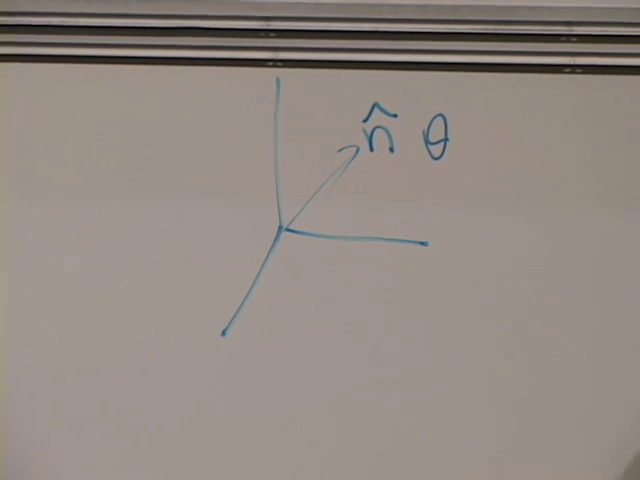
\includegraphics[width=0.58\textwidth]{lecture_03_figure_02.png}\caption{Un eje \(\hat{\boldsymbol n}\) y un ángulo \(\theta\) especifican una rotación espacial.}\lectureframe{00:02:34}\end{figure}

Una dirección sobre la esfera unidad requiere dos parámetros, como la longitud y la latitud. El ángulo alrededor de esa dirección aporta un tercero. Por tanto, las rotaciones forman una familia de tres parámetros. Por ahora no nos ocuparemos de las identificaciones globales debidas a ángulos que difieren en \(2\pi\); aquí importa el número local de parámetros.

La descripción mediante eje y ángulo tiene cierta redundancia. Invertir el eje e invertir el ángulo da la misma operación, y los ángulos suficientemente grandes pueden reducirse módulo una vuelta completa. Nada de esto cambia el hecho de que, cerca de la identidad, una rotación tiene tres parámetros que varían continuamente. Más adelante compararemos ese número local con el de parámetros independientes de una representación matricial.

Las propiedades de grupo pueden comprobarse una por una:
\begin{enumerate}
\item \emph{Clausura.} Realizar dos rotaciones sucesivas produce otra rotación.
\item \emph{Identidad.} La operación de no hacer nada es la rotación identidad.
\item \emph{Inverso.} Una rotación de ángulo \(\theta\) alrededor de \(\hat{\boldsymbol n}\) se deshace mediante una rotación de ángulo \(-\theta\) alrededor del mismo eje.
\item \emph{Asociatividad.} Tres rotaciones sucesivas satisfacen
\[
(R_1R_2)R_3=R_1(R_2R_3).
\]
\end{enumerate}

Las rotaciones no son conmutativas. En general, una rotación alrededor del eje \(x\) seguida de otra alrededor del eje \(y\) produce una orientación distinta de la que resulta al realizar las mismas dos operaciones en orden inverso:
\begin{equation}
R_x(\alpha)R_y(\beta)\ne R_y(\beta)R_x(\alpha).
\end{equation}
La diferencia es de segundo orden cuando ambos ángulos son muy pequeños; por eso las rotaciones infinitesimales pueden parecer casi conmutativas. Aun así, el grupo completo no es abeliano.

La falta de conmutatividad puede comprobarse sin ecuaciones. Tomen un libro o una caja, marquen una cara como frente y gírenlo noventa grados alrededor del eje \(x\) y luego noventa grados alrededor del eje \(y\). Vuelvan a la orientación inicial e inviertan el orden. La cara marcada acaba apuntando en otra dirección. Con ángulos pequeños, la discrepancia es más difícil de apreciar, pero no desaparece: comienza en el producto de los dos ángulos pequeños.

\begin{classroomqa}\audiencequestion{¿Estas rotaciones son sucesivas, en lugar de simultáneas?\lecturetimestamp{00:04:45}}\lecturerresponse{Sí. La multiplicación de grupo significa realizar una operación y luego otra. El orden de esas rotaciones sucesivas es precisamente lo que puede impedir la conmutatividad.}\end{classroomqa}

Este es nuestro primer grupo no abeliano. La aplicación que nos interesa finalmente no es el color de un objeto ordinario, sino los estados de color rojo, verde y azul de un quark. Se trata de un sistema interno de tres estados, cuyas transformaciones interesantes mezclan los tres colores. Las rotaciones ordinarias ofrecen un modelo familiar de cómo un grupo continuo actúa mediante matrices.

Un grupo por sí solo es abstracto. Para usarlo en física, debemos especificar sobre qué objetos actúa. Una {representación} asigna un operador o una matriz a cada elemento del grupo, de modo que el producto de elementos del grupo se reproduzca mediante el producto de las matrices asignadas. Distintos objetos físicos pueden tener distintas representaciones del mismo grupo. Los vectores y los estados de espín uno y de espín un medio serán tres ejemplos.

\section{La representación vectorial tridimensional}

Sea un vector ordinario de componentes
\begin{equation}
\boldsymbol V=(V_x,V_y,V_z),\qquad V_i,\quad i=1,2,3.
\end{equation}
Se puede rotar el vector físico manteniendo fijos los ejes, o rotar los ejes de coordenadas manteniendo fijo el vector. Las convenciones difieren, pero en ambas descripciones los componentes se mezclan mediante una matriz \(3\times3\). Para cada par de eje y ángulo \((\hat{\boldsymbol n},\theta)\), escribimos
\begin{equation}
V_i'=R_{ij}(\hat{\boldsymbol n},\theta)V_j,
\label{eq:l3-vector-rotation}
\end{equation}
donde se suma sobre los índices repetidos.

El índice repetido \(j\) es un índice mudo. La ecuación~\eqref{eq:l3-vector-rotation} significa explícitamente
\begin{equation}
V_i'=R_{i1}V_1+R_{i2}V_2+R_{i3}V_3
\end{equation}
para cada componente de salida \(i\). El índice libre \(i\) indica qué componente se calcula; se suma sobre el índice repetido \(j\), que puede cambiarse de nombre sin alterar la ecuación. Mantener separados estos dos papeles evita la mayoría de los errores de índices en el argumento de conservación de la longitud.

\begin{figure}[htbp]\centering
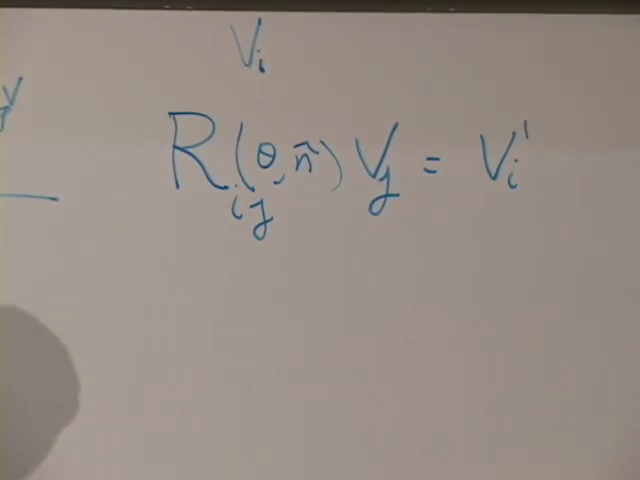
\includegraphics[width=0.68\textwidth]{lecture_03_figure_03.png}\caption{Una matriz de rotación transforma los componentes originales del vector en los componentes rotados.}\lectureframe{00:07:41}\end{figure}

Una rotación genuina conserva la longitud. Por ahora, tanto \(V_i\) como \(R_{ij}\) son reales, así que
\begin{equation}
V_i'V_i'=V_iV_i
\end{equation}
para cualquier vector. Para obtener la condición matricial, escribamos la misma transformación con índices mudos distintos:
\begin{equation}
V_i'=R_{ij}V_j,\qquad V_i'=R_{ik}V_k.
\end{equation}
Al multiplicar y sumar sobre \(i\), se obtiene
\begin{align}
V_i'V_i'
 &=R_{ij}V_jR_{ik}V_k\\
 &=R_{ij}R_{ik}V_jV_k.
\end{align}
Esto es igual a \(V_jV_j\) para cualquier elección de \(V\) solo si
\begin{equation}
R_{ij}R_{ik}=\delta_{jk}.
\label{eq:l3-orthogonality-index}
\end{equation}
En notación matricial,
\begin{equation}
R^TR=\boldsymbol 1,
\label{eq:l3-orthogonal}
\end{equation}
y, por tanto,
\begin{equation}
R^{-1}=R^T.
\end{equation}
La transposición simplemente intercambia las filas y las columnas.

¿Por qué el coeficiente debe ser \(\delta_{jk}\)? La delta de Kronecker fija \(j=k\) en la suma:
\begin{equation}
\delta_{jk}V_jV_k=V_1^2+V_2^2+V_3^2.
\end{equation}
Si \(R_{ij}R_{ik}\) fuera distinto de \(\delta_{jk}\), alguna dirección o algún término cruzado \(V_jV_k\) modificaría la longitud. Como la igualdad debe cumplirse para todo vector posible, y no solo para uno elegido, el coeficiente matricial debe ser la identidad.

La ecuación~\eqref{eq:l3-orthogonal} es la condición de ortogonalidad que define esta representación matricial real. El producto de las matrices reproduce la ley de composición de las rotaciones espaciales. Esta no es la única representación del grupo de rotaciones; simplemente es la más fácil de visualizar.

La relación del inverso tiene un significado geométrico inmediato. Se puede deshacer una rotación sin resolver una nueva ecuación matricial: basta intercambiar filas y columnas. Si \(R_1\) y \(R_2\) representan dos rotaciones, entonces \(R_2R_1\) representa su acción sucesiva y también es ortogonal. Así, las operaciones matriciales conservan la misma estructura de clausura, identidad, inverso y asociatividad establecida geométricamente.

\section{Espín uno y la representación vectorial}

La representación tridimensional también actúa sobre estados cuánticos. Una partícula de espín uno tiene tres proyecciones de espín posibles:
\begin{equation}
m=+1,\quad 0,\quad -1.
\end{equation}
Por tanto, su estado de espín es una columna de tres componentes formada por amplitudes de probabilidad. Al rotar la partícula, o al cambiar la orientación del campo magnético que define el eje de espín, esas tres amplitudes se mezclan mediante una representación tridimensional del grupo de rotaciones.

El número de estados de espín sigue la regla conocida \(2s+1\). El espín cero tiene un estado, el espín un medio tiene dos, el espín uno tiene tres y el espín tres medios tiene cuatro. Por tanto, la dimensión del vector de estado cambia con el espín. La misma rotación física debe representarse mediante matrices de tamaños distintos cuando actúa en esos diferentes espacios de estados.

Para una partícula de espín uno, elijamos la base
\begin{equation}
\lvert 1,+1\rangle,qquad
\lvert 1,0\rangle,qquad
\lvert 1,-1\rangle.
\end{equation}
Un estado es
\begin{equation}
\lvert\psi\rangle
=c_{+}\lvert1,+1\rangle+c_0\lvert1,0\rangle+c_{-}\lvert1,-1\rangle.
\end{equation}
Al rotar el aparato no se crea un cuarto estado de espín; los tres coeficientes \(c_+,c_0,c_-\) se mezclan entre sí. Por tanto, el operador de rotación correspondiente debe ser una matriz \(3\times3\).

Para el espín uno, esta representación se transforma igual que un vector espacial ordinario. Ese es el significado preciso de llamar \emph{partícula vectorial} a una partícula de espín uno: sus tres amplitudes de espín y las tres componentes de un vector obedecen la misma ley de rotación. No es necesario imaginar el estado cuántico como una flecha literal; la afirmación se refiere a cómo se mezclan sus componentes.

Esta correspondencia no es accidental. Un vector tridimensional y un estado de espín uno llevan representaciones tridimensionales equivalentes del grupo de rotaciones. La expresión {partícula vectorial} resume esa propiedad de transformación. No afirma que exista dentro de la partícula una diminuta flecha rígida que represente el estado de polarización cuántico.

\section{Simetrías discretas y continuas}

Antes de pasar al espín un medio, conviene distinguir dos grandes tipos de grupos. Una reflexión es un ejemplo discreto sencillo. Está la identidad y está la reflexión \(P\): o bien se invierte la orientación, o bien no. En cambio, una fase
\begin{equation}
e^{i\phi}
\end{equation}
depende continuamente de \(\phi\), y una rotación espacial depende continuamente de su eje y su ángulo. Estos grupos continuos se llaman \emph{grupos de Lie}, por Sophus Lie; el nombre se pronuncia \emph{«li»}. Las simetrías continuas serán nuestra principal preocupación, aunque las simetrías discretas también son importantes.

Para el grupo de dos elementos de reflexión,
\begin{equation}
P^2=1.
\end{equation}
no hay una cantidad de reflexión que pueda variarse continuamente entre \(1\) y \(P\). Un grupo de fases es distinto: entre \(e^{i\phi_1}\) y \(e^{i\phi_2}\) hay continuamente muchas otras fases. Las rotaciones espaciales tienen el mismo carácter continuo, pero, a diferencia de \(U(1)\), no son abelianas.

El espín cero da la representación más sencilla del grupo de rotaciones. Un estado de espín cero permanece inalterado bajo cualquier rotación, por lo que a cada elemento del grupo le corresponde la identidad unidimensional:
\begin{equation}
D^{(0)}(R)=1.
\end{equation}
El propio grupo sigue teniendo infinitas rotaciones; lo trivial es la representación sobre el estado de espín cero.

Es esencial distinguir entre un grupo y una de sus representaciones. El grupo de rotaciones no se reduce a un grupo de un solo elemento cada vez que actúa sobre un escalar. Más bien, cada uno de sus elementos se representa mediante el mismo número \(1\) en ese escalar particular.

\section{Un estado general de espín un medio}

Un sistema de espín un medio tiene dos estados de base. Respecto de un eje \(z\),
\begin{equation}
\lvert\uparrow\rangle=
\begin{pmatrix}1\\0\end{pmatrix},
\qquad
\lvert\downarrow\rangle=
\begin{pmatrix}0\\1\end{pmatrix}.
\end{equation}
Un estado general es un espinor de dos componentes:
\begin{equation}
\lvert\psi\rangle=
\begin{pmatrix}\alpha_1\\\alpha_2\end{pmatrix},
\qquad
|\alpha_1|^2+|\alpha_2|^2=1.
\label{eq:l3-spinor}
\end{equation}
Las entradas son complejas. La elección \((\alpha_1,\alpha_2)=(1,0)\) corresponde al espín hacia arriba, y \((0,1)\) al espín hacia abajo. Una combinación normalizada general describe un espín polarizado en alguna otra dirección.

Las palabras {arriba} y {abajo} solo tienen sentido una vez elegido un eje. Aquí, ese eje es \(z\). Un eje de medida distinto tiene otro par de estados de base, y un estado definido como arriba respecto de un eje suele aparecer como una superposición en otra base. Al rotar el espín físico o los ejes de referencia, los coeficientes cambian en consecuencia.

Dos amplitudes complejas contienen cuatro parámetros reales. La normalización elimina uno y la fase global físicamente irrelevante elimina otro, de modo que quedan dos parámetros reales. Ese es exactamente el número necesario para elegir una dirección sobre una esfera. Para estudiar las rotaciones no hace falta deducir la correspondencia explícita entre \((\alpha_1,\alpha_2)\) y esa dirección.

La fase global se elimina porque
\begin{equation}
\begin{pmatrix}\alpha_1\\\alpha_2\end{pmatrix}
\quad\hbox{and}\quad
e^{i\chi}
\begin{pmatrix}\alpha_1\\\alpha_2\end{pmatrix}
\end{equation}
representan el mismo rayo físico. La normalización fija la probabilidad total, no una dirección en el espacio euclidiano ordinario. Tras ambas identificaciones, los dos parámetros restantes pueden interpretarse como los ángulos polar y azimutal de la dirección de polarización del espín.

Al rotar el espín, su estado pasa a ser
\begin{equation}
\alpha_i'=U_{ij}\alpha_j,
\qquad
\begin{pmatrix}\alpha_1'\\\alpha_2'\end{pmatrix}
=
\begin{pmatrix}
U_{11}&U_{12}\\
U_{21}&U_{22}
\end{pmatrix}
\begin{pmatrix}\alpha_1\\\alpha_2\end{pmatrix}.
\label{eq:l3-spinor-transform}
\end{equation}
Así, las rotaciones espaciales tienen una representación matricial bidimensional que actúa sobre espinores. En esta representación hay una ambigüedad global de dos valores que dejaremos para más adelante; localmente, las matrices tienen las propiedades de transformación que necesitamos a continuación.

El par transformado \((\alpha_1',\alpha_2')\) debe seguir siendo un estado cuántico posible. Por tanto, la primera pregunta sobre \(U\) no se refiere a su fórmula explícita en función del eje y el ángulo, sino a la condición de que conserve la normalización de cualquier espinor de entrada.

\section{Conservación de la probabilidad y matrices unitarias}

Una rotación debe transformar un estado normalizado en otro estado normalizado:
\begin{equation}
\alpha_i^*\alpha_i=\alpha_i'^*\alpha_i'=1.
\end{equation}
Al sustituir la ecuación~\eqref{eq:l3-spinor-transform},
\begin{align}
\alpha_i'^*\alpha_i'
 &=(U_{ij}\alpha_j)^*(U_{ik}\alpha_k)\\
 &=\alpha_j^*U_{ij}^*U_{ik}\alpha_k.
\end{align}
se obtiene para los vectores reales la condición análoga
\begin{equation}
(U^T)^*U=\boldsymbol 1.
\end{equation}
La transposición seguida de la conjugación compleja es la conjugada hermítica:
\begin{equation}
U^\dagger=(U^T)^*,
\end{equation}
Por tanto, la condición de conservación de la normalización es
\begin{equation}
U^\dagger U=\boldsymbol 1.
\label{eq:l3-unitarity}
\end{equation}

La conjugación compleja adicional es el único cambio esencial respecto del cálculo con vectores reales. Para un vector real, \(V_iV_i\) es una longitud. Para un espinor, \(\alpha_i^*\alpha_i\) es una probabilidad. Se necesita la conjugación compleja para que esa probabilidad sea real y no negativa, así que la transposición se sustituye por la conjugada hermítica.

La ecuación~\eqref{eq:l3-unitarity} también da inmediatamente el inverso:
\begin{equation}
U^{-1}=U^\dagger.
\end{equation}
Por tanto, la rotación inversa conserva la misma norma de probabilidad. Al igual que las matrices de rotación ordinarias, los productos de matrices unitarias siguen siendo unitarios, de modo que la representación respeta la multiplicación del grupo.

\begin{figure}[htbp]\centering
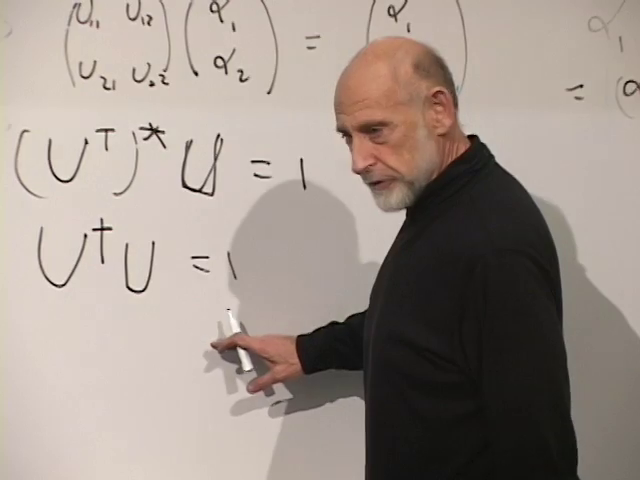
\includegraphics[width=0.62\textwidth]{lecture_03_figure_04.png}\caption{La matriz de rotación del espinor satisface \(U^\dagger U=\boldsymbol 1\).}\lectureframe{00:27:41}\end{figure}

Las matrices que satisfacen la ecuación~\eqref{eq:l3-unitarity} son unitarias. Una matriz compleja general \(2\times2\) comienza con ocho parámetros reales. La ecuación matricial de unitariedad \(2\times2\) impone cuatro restricciones reales independientes, con lo que quedan cuatro parámetros. Una rotación espacial solo tiene tres. Hace falta una restricción más para aislar la representación espinorial de las rotaciones de todas las matrices de \(U(2)\).

Las cuatro restricciones también pueden apreciarse al considerar las dos columnas de \(U\) como dos vectores complejos. Cada columna debe tener norma unitaria, lo cual aporta dos condiciones reales; además, las columnas deben ser ortogonales, lo cual aporta una condición compleja, o dos reales. En total, son cuatro. El cuarto parámetro restante en \(U(2)\) resultará ser una fase global del determinante, y no una nueva rotación espacial.

\section{Determinante uno y \texorpdfstring{\(SU(2)\)}{SU(2)}}

La condición adicional es
\begin{equation}
\det U=1.
\label{eq:l3-det-one}
\end{equation}
Es compatible con la multiplicación de grupo porque
\begin{equation}
\det(AB)=\det A\,\det B.
\end{equation}
El producto de dos matrices unitarias de determinante uno vuelve a tener determinante uno, y la identidad también tiene determinante uno. Estas matrices forman un subgrupo cerrado.

El inverso también pertenece al subgrupo. Si \(\det U=1\), entonces
\begin{equation}
\det U^{-1}=\frac{1}{\det U}=1.
\end{equation}
Así, imponer que el determinante sea uno no elimina la identidad, no rompe la clausura ni hace perder los inversos. Selecciona de forma coherente un grupo con un parámetro continuo menos.

La unitariedad por sí sola implica
\begin{equation}
\det(U^\dagger U)=
(\det U)^*\det U
=|\det U|^2=1.
\end{equation}
No obliga a que \(\det U\) sea \(+1\) o \(-1\). El determinante de una matriz unitaria general puede ser cualquier fase:
\begin{equation}
\det U=e^{i\phi},
\qquad
\det U^\dagger=e^{-i\phi}.
\end{equation}
La condición~\eqref{eq:l3-det-one} fija esa fase, que de otro modo sería libre, y elimina un parámetro real.

\begin{classroomqa}\audiencequestion{¿La condición \(U^\dagger U=\boldsymbol 1\), sin imponer que el determinante sea uno, obliga a que \(\det U^\dagger\) sea igual a \(\det U\) o a que solo pueda ser \(+1\) o \(-1\)?\lecturetimestamp{00:31:21}}\lecturerresponse{No. Los dos determinantes son complejos conjugados. Pueden ser \(e^{i\phi}\) y \(e^{-i\phi}\), cuyo producto es uno. La restricción de unitariedad especial obliga entonces a que ambos sean uno.}\end{classroomqa}

Las matrices unitarias \(n\times n\) forman \(U(n)\). Para \(n=1\), una matriz unitaria es simplemente la fase \(e^{i\phi}\), que da lugar a \(U(1)\). El subgrupo de determinante uno es el \emph{grupo unitario especial}:
\begin{equation}
SU(n)=\{U\in U(n):\det U=1\}.
\end{equation}
El espinor de dos componentes está sometido a la acción de \(SU(2)\), un grupo de tres parámetros.

La notación indica ambas restricciones: \(U\) significa unitario y \(S\) significa especial, es decir, de determinante uno. Estos grupos unitarios especiales aparecen repetidamente porque conservan un producto interno complejo y excluyen la fase común independiente que aporta el determinante.

Localmente, \(SU(2)\) tiene el mismo álgebra de rotaciones y la estructura de multiplicación necesaria para rotar estados de espín un medio. Globalmente, hay que recordar el matiz que dejamos pendiente: \(SU(2)\) es el recubrimiento doble del grupo de rotaciones ordinarias \(SO(3)\), así que dos elementos de \(SU(2)\) corresponden a una misma rotación espacial.\editorialnote{La formulación mediante el recubrimiento doble precisa la ambigüedad de dos valores mencionada, pero no desarrollada, en el texto original.}

\section{Rotaciones infinitesimales y matrices de Pauli}

\begin{classroomqa}\audiencequestion{¿Dónde aparecen en esta construcción las matrices de espín, o matrices de Pauli?\lecturetimestamp{00:33:16}}\lecturerresponse{Aparecen cuando se toma un elemento del grupo muy cerca de la identidad, lo que corresponde a una rotación de ángulo muy pequeño. Son los generadores de esas rotaciones infinitesimales.}\end{classroomqa}

Partamos de
\begin{equation}
U=\boldsymbol 1+\epsilon M+O(\epsilon^2),
\label{eq:l3-small-u-anti}
\end{equation}
donde \(\epsilon\) es real y pequeño. Entonces
\begin{equation}
U^\dagger=\boldsymbol 1+\epsilon M^\dagger+O(\epsilon^2),
\end{equation}
y la unitariedad da
\begin{align}
U^\dagger U
 &=\boldsymbol 1+\epsilon(M^\dagger+M)+O(\epsilon^2).
\end{align}
Al primer orden,
\begin{equation}
M^\dagger=-M.
\end{equation}
Así, la matriz \(M\) de la ecuación~\eqref{eq:l3-small-u-anti} es antihermítica.

Solo se conservan los términos lineales en \(\epsilon\). Se descarta el producto \(\epsilon^2M^\dagger M\) porque es de segundo orden. Esta es la ventaja de trabajar cerca de la identidad: las condiciones no lineales del grupo se convierten en condiciones lineales para sus generadores.

Es más conveniente extraer un factor de \(i\):
\begin{equation}
U=\boldsymbol 1+i\epsilon H+O(\epsilon^2).
\label{eq:l3-small-u-herm}
\end{equation}
La conjugación compleja transforma \(i\) en \(-i\), de modo que
\begin{equation}
U^\dagger=\boldsymbol 1-i\epsilon H^\dagger+O(\epsilon^2).
\end{equation}
Ahora,
\begin{equation}
U^\dagger U
=\boldsymbol 1+i\epsilon(H-H^\dagger)+O(\epsilon^2),
\end{equation}
y la unitariedad al primer orden exige
\begin{equation}
H^\dagger=H.
\end{equation}
Al dejar explícito el factor de \(i\), el generador resulta hermítico.

La multiplicación por \(i\) no ha cambiado las matrices infinitesimales permitidas; solo ha cambiado la convención para denominar el generador. En física se suelen elegir generadores hermíticos porque sus valores propios son reales y porque los observables asociados, como el momento angular, son hermíticos.

La condición de determinante uno implica que la traza sea nula.\editorialnote{El desarrollo verbal del determinante contiene un breve error en los subíndices. El término lineal corregido es \(A_{11}+A_{22}=\operatorname{tr}A\); los productos de elementos no diagonales empiezan en segundo orden.}. Para una matriz \(2\times2\) pequeña \(A\),
\begin{equation}
\det(\boldsymbol 1+A)
=
\det
\begin{pmatrix}
1+A_{11}&A_{12}\\
A_{21}&1+A_{22}
\end{pmatrix}.
\end{equation}
Al desarrollar,
\begin{align}
\det(\boldsymbol 1+A)
 &=(1+A_{11})(1+A_{22})-A_{12}A_{21}\\
 &=1+A_{11}+A_{22}+O(A^2)\\
 &=1+\operatorname{tr}A+O(A^2).
\end{align}
Al aplicar esto a \(A=i\epsilon H\),
\begin{equation}
\det U=1+i\epsilon\,\operatorname{tr}H+O(\epsilon^2).
\end{equation}
Por tanto, \(\det U=1\) exige
\begin{equation}
\operatorname{tr}H=0.
\end{equation}
La condición sobre la traza elimina precisamente el generador proporcional a la matriz identidad. Una matriz hermítica general \(2\times2\) tiene cuatro parámetros reales: dos elementos diagonales reales y un elemento no diagonal complejo. La traza fija una combinación real y deja tres parámetros. Esto coincide con los tres ejes alrededor de los cuales puede realizarse una rotación espacial infinitesimal.

Así pues, los generadores infinitesimales de \(SU(2)\) son matrices hermíticas \(2\times2\) de traza nula. Las tres matrices de Pauli forman una base:
\begin{equation}
\begin{aligned}
\sigma_x&=
\begin{pmatrix}0&1\\1&0\end{pmatrix},
&
\sigma_y&=
\begin{pmatrix}0&-i\\i&0\end{pmatrix},
\\[0.4em]
\sigma_z&=
\begin{pmatrix}1&0\\0&-1\end{pmatrix}.
\end{aligned}
\end{equation}
Todo generador puede escribirse
\begin{equation}
H=a_x\sigma_x+a_y\sigma_y+a_z\sigma_z.
\end{equation}
Una rotación pequeña alrededor del eje \(x\) selecciona \(\sigma_x\); una alrededor del eje \(y\) selecciona \(\sigma_y\); y una rotación alrededor de cualquier otro eje selecciona la combinación lineal correspondiente. En unidades en las que \(\hbar=1\), los operadores de espín son
\begin{equation}
S_i=\frac{\sigma_i}{2}.
\end{equation}

Por ejemplo, un eje a medio camino entre \(x\) y \(y\) usa un generador proporcional a
\begin{equation}
\frac{\sigma_x+\sigma_y}{\sqrt2}.
\end{equation}
La dirección del vector de coeficientes \((a_x,a_y,a_z)\) selecciona el eje de rotación, mientras que su magnitud, junto con \(\epsilon\), determina el ángulo pequeño. Esta es la conexión entre las matrices de espín que aparecen en los conmutadores de momento angular y los operadores de rotación finita. En particular,
\begin{equation}
[S_x,S_y]=iS_z
\end{equation}
y sus permutaciones cíclicas codifican la falta de conmutatividad que ya vimos geométricamente. La rotación finita estándar se obtiene al exponenciar el generador infinitesimal\editorialnote{La fórmula exponencial de la rotación finita completa la construcción infinitesimal de la forma habitual; la fuente solo deduce las condiciones para los generadores y su base de matrices de Pauli.}:
\begin{equation}
U(\hat{\boldsymbol n},\theta)
=\exp\left(-\frac{i\theta}{2}\,
\hat{\boldsymbol n}\cdot\boldsymbol\sigma\right).
\end{equation}\section{Un espacio de color de tres estados}

Podemos dejar para más adelante la combinación de representaciones. Ahora dejaremos atrás el espín espacial y volveremos al color de los quarks. Un quark sigue teniendo espín un medio, pero su color es un grado de libertad independiente de tres estados:
\begin{equation}
\lvert r\rangle,\qquad
\lvert g\rangle,\qquad
\lvert b\rangle.
\end{equation}
Un estado de color general es
\begin{equation}
\begin{aligned}
\lvert q\rangle_{\mathrm{color}}
={}&
\alpha_r\lvert r\rangle
+\alpha_g\lvert g\rangle
+\alpha_b\lvert b\rangle,
\\
&|\alpha_r|^2+|\alpha_g|^2+|\alpha_b|^2=1.
\end{aligned}
\end{equation}
Equivalentemente,
\begin{equation}
q=
\begin{pmatrix}
\alpha_r\\
\alpha_g\\
\alpha_b
\end{pmatrix}.
\end{equation}
Los módulos al cuadrado son las probabilidades de encontrar los colores rojo, verde y azul en una base de color elegida. La misma notación de triplete permite reunir tres operadores de campo de quark:
\begin{equation}
\psi=
\begin{pmatrix}
\psi_r\\
\psi_g\\
\psi_b
\end{pmatrix}.
\end{equation}

Hay que mantener conceptualmente separados el espín y el color. La etiqueta de espín indica cómo se transforma el estado bajo rotaciones del espacio físico. La etiqueta de color indica cómo se transforma bajo una simetría interna que no rota el laboratorio. Un estado de quark lleva ambas etiquetas, aunque en esta discusión se omite el espín para centrarnos en el color.

Escribir tres operadores de campo en una sola columna es más que una ayuda para organizar la información. Permite expresar la simetría mediante una sola ecuación matricial. Una transformación puede convertir un campo rojo en una combinación lineal de campos rojos, verdes y azules, del mismo modo que una rotación espacial convierte una componente de un vector en una combinación lineal de sus otras componentes.

Primero podemos imaginar transformaciones discretas que intercambian dos colores. La simetría más amplia contiene mezclas continuas de los tres. Una matriz de intercambio sencilla puede requerir una fase adicional para que su determinante sea uno; así, el intercambio queda incorporado en el grupo unitario especial.

Para dos estados de base, el intercambio simple se representa mediante
\begin{equation}
X=
\begin{pmatrix}0&1\\1&0\end{pmatrix},
\qquad
\det X=-1.
\end{equation}
Al multiplicar toda la matriz por \(i\), se obtiene
\begin{equation}
\det(iX)=i^2\det X=1.
\end{equation}
Por tanto, con una elección coherente de la fase, el intercambio discreto puede aparecer como un elemento particular del grupo continuo más amplio.

\begin{classroomqa}\audiencequestion{¿Una matriz que simplemente intercambia dos estados de base tiene un determinante inadecuado para \(SU(2)\)?\lecturetimestamp{00:43:46}}\lecturerresponse{El intercambio simple tiene determinante \(-1\). Un factor adecuado de \(i\) da una matriz representativa de determinante uno, de modo que el intercambio puede incluirse entre las transformaciones unitarias especiales continuas.}\end{classroomqa}

\section{\texorpdfstring{\(SU(3)\)}{SU(3)} y los ocho generadores de color}

La transformación continua de color es
\begin{equation}
\begin{aligned}
q'&=Uq,
&
U^\dagger U&=\boldsymbol 1,
\\
\det U&=1,
&
U&\in SU(3).
\end{aligned}
\label{eq:l3-su3-action}
\end{equation}
Las matemáticas son las mismas que en la construcción unitaria especial usada para espinores, pero ahora \(U\) es \(3\times3\). No se trata de una rotación del espacio físico, sino de una rotación en el espacio interno de color.

La unitariedad conserva la normalización del estado de color:
\begin{equation}
q^\dagger q
=|\alpha_r|^2+|\alpha_g|^2+|\alpha_b|^2.
\end{equation}
El determinante uno elimina la dirección de fase común \(U(1)\) del espacio de mezclas continuas. Las matrices resultantes pueden realizar intercambios sencillos, cambios de fase relativos y superposiciones genuinamente continuas, y todas pertenecen a un mismo grupo cerrado.

El número de parámetros se obtiene de inmediato. Una matriz compleja \(3\times3\) tiene nueve elementos complejos, es decir, dieciocho parámetros reales. La ecuación matricial \(U^\dagger U=\boldsymbol 1\) impone nueve condiciones reales. El determinante uno elimina una más:
\begin{equation}
\dim SU(3)=18-9-1=8.
\end{equation}
Así pues, \(SU(3)\) tiene ocho generadores infinitesimales independientes.

Las nueve condiciones reales de unitariedad también pueden entenderse considerando las columnas de \(U\). Tres columnas complejas deben tener cada una norma unitaria y, además, cada par debe ser ortogonal. Estas condiciones eliminan nueve de los dieciocho parámetros reales iniciales. La fase del determinante elimina el décimo y deja ocho. Este es el análogo para tres estados del recuento \(8-4-1=3\) correspondiente a \(SU(2)\).

La aparición del 8 es el mismo hecho que, en última instancia, da lugar a las 8 especies de gluones. Decir que no hay 9 gluones porque la restricción del determinante eliminó una dirección es solo una regla mnemotécnica. Con mayor precisión, las 9 matrices de color-anticolor se descomponen en una dirección singlete de color, proporcional a la identidad, y 8 direcciones sin traza. Los 8 generadores sin traza forman la estructura de color adjunta que portan los gluones de la QCD.\editorialnote{La formulación singlete más octete es la versión precisa estándar de la observación deliberadamente heurística de la fuente sobre el determinante; la construcción del campo gauge se desarrolla más adelante.}

En esta etapa, la relación con los 8 gluones es un anticipo, no una derivación completa. Para obtener partículas gauge, hay que promover la simetría de color a una simetría local y determinar los campos compensadores. Lo que ya ha mostrado el recuento de parámetros es que hay 8 direcciones independientes en las que una transformación de color \(SU(3)\) puede empezar a apartarse de la identidad.

\section{La simetría de color impone restricciones a la QCD}

La afirmación básica sobre la simetría es que la física permanece invariante bajo la transformación de color de la ecuación~\eqref{eq:l3-su3-action}. Esta es la simetría interna central de la cromodinámica cuántica. Mezclar las componentes de color es, en cuanto a su forma, análogo a mezclar las amplitudes de espín arriba y espín abajo; a su vez, esas transformaciones de espinor están relacionadas con rotaciones de direcciones espaciales, pero no deben confundirse estos tres espacios.

Decir que el color es una simetría significa que cambiar la base de color no altera las predicciones físicas. Rojo, verde y azul son nombres convenientes para tres vectores de base, no tres pigmentos observables. Una rotación simultánea \(SU(3)\) de las componentes de color debe dejar inalterada la forma de las leyes. Esta invariancia no es un rasgo estético opcional, sino el principio organizador de la QCD.

La simetría restringe el lagrangiano. En el ejemplo anterior de \(U(1)\), la invariancia bajo una transformación de fase común restringía los términos permitidos a aquellos que contenían factores equilibrados de un campo y su conjugado. En la QCD, del mismo modo, todos los términos deben ser invariantes bajo la transformación de color \(SU(3)\). Este requisito tiene consecuencias para las interacciones, las cantidades conservadas y la forma del campo de gluones.

Supongamos que un término propuesto tiene un índice de color libre. Bajo la ecuación~\eqref{eq:l3-su3-action}, ese índice rota, por lo que el término no puede ser invariante por sí solo. Los términos permitidos deben contraer los índices de color en combinaciones invariantes o usar campos gauge cuyas transformaciones compensen el cambio. Esta es la consecuencia práctica del principio de simetría: descarta acoplamientos arbitrarios y organiza las interacciones que sí se permiten.

La construcción completa de la QCD requiere un paso más: hay que permitir que la transformación de color varíe de un punto a otro, y el campo gauge debe compensar ese cambio local.\editorialnote{Localizar la simetría de color es la formulación gauge estándar de la discusión global de \(SU(3)\); esta lección de la fuente no desarrolla el tema.} Ese desarrollo corresponde a la etapa siguiente. Por ahora, la estructura esencial ya está establecida: un triplete de color sobre el que actúa una simetría unitaria especial de tres estados con 8 generadores.

Por el momento, el cálculo ha llegado tan lejos en la teoría de grupos como hace falta. Partimos de rotaciones que pueden representarse en el espacio ordinario, pasamos a las matrices que actúan sobre vectores y espinores, y luego aplicamos la misma lógica a un espacio interno de color. El siguiente paso puede volver a la física de partículas con el marco matemático ya disponible, en vez de exigirle al formalismo que sostenga por sí solo toda la explicación física.
\chapter{Representaciones de color, hadrones y confinamiento}

\paragraph{Un breve interludio inicial.}
Antes de volver a la teoría de grupos, permítanme un descarado anuncio comercial. \emph{La guerra de los agujeros negros} cuenta la larga discusión con Stephen Hawking sobre si los agujeros negros destruyen la información cuántica. También relata una crueldad propia de los físicos teóricos: no solo el gato de Schrödinger, sino también el pez de Susskind y su desafortunado viaje por el retrete. Cumplido ese deber, volvamos a Alice y Bob. Alice sigue sufriendo, porque Bob todavía la obliga a aprender teoría de grupos.

\lectureoverview{Una simetría se vuelve física por medio de su acción sobre los estados. Empezaremos con las rotaciones para introducir las representaciones y los generadores; después repetiremos la construcción para el color \(SU(3)\). Las representaciones de color se combinan para formar hadrones, y su dinámica explica por qué nunca se observa color aislado.}

\section{El grupo y los objetos sobre los que actúa}

En toda discusión sobre simetrías hay dos ideas. Primero, un grupo abstracto: un conjunto de operaciones con una ley de multiplicación, un elemento identidad e inversos. Segundo, los objetos sobre los que actúan esas operaciones. Se pueden distinguir ambas ideas, pero en física no se pueden separar. Una simetría importa porque transforma estados físicos, campos, coordenadas u observables.

\begin{classroomqa}
\audiencequestion{Se ha descrito un grupo tanto como una tabla de multiplicación abstracta como mediante matrices que actúan sobre objetos físicos. ¿Se pueden disociar esas dos partes?
\lecturetimestamp{00:01:58}}
\lecturerresponse{Son niveles de descripción distintos, pero están completamente relacionados. Una rotación existe como operación abstracta antes de especificar qué rota. La física pregunta entonces cómo actúa esa misma operación sobre los estados y las magnitudes pertinentes para un sistema concreto. Las matrices proporcionan esa acción concreta y, a la vez, preservan la ley de multiplicación abstracta.}
\end{classroomqa}

Las rotaciones espaciales ofrecen el ejemplo más sencillo. En la mecánica clásica, una misma rotación puede actuar sobre las coordenadas de una partícula, sobre la dirección de un imán o sobre cualquier otro vector. En mecánica cuántica, los estados pertenecen a un espacio vectorial lineal, así que una rotación se representa mediante un operador lineal sobre ese espacio. Si \(g\) denota un elemento abstracto del grupo y \(D(g)\) su matriz representante, la consistencia exige que
\begin{equation}
D(g_1g_2)=D(g_1)D(g_2),
\qquad
D(e)=\boldsymbol 1.
\end{equation}
Las matrices no tienen por qué parecerse a las operaciones abstractas, pero su multiplicación debe reproducir la multiplicación del grupo.
\editorialnote{La ecuación de homomorfismo expresa explícitamente la correspondencia entre la multiplicación de grupo y la multiplicación de matrices que la fuente describe verbalmente.}

La dimensión de la matriz viene determinada por el espacio de estados, no solo por el grupo abstracto. Si conservamos únicamente el espín de un electrón, hay dos posibilidades ortogonales, espín hacia arriba y espín hacia abajo, y un estado es un vector columna de dos componentes. Por tanto, las rotaciones actúan mediante matrices \(2\times2\). Para dos objetos de espín un medio hay cuatro estados de base,
\begin{equation}
\ket{\uparrow\uparrow},\qquad
\ket{\uparrow\downarrow},\qquad
\ket{\downarrow\uparrow},\qquad
\ket{\downarrow\downarrow},
\end{equation}
y la acción inducida sobre el espacio combinado es tetradimensional.

La secuencia conocida es
\begin{equation}
\begin{array}{c|c|c}
\text{spin} & \text{number of states} & \text{matrix dimension}\\
\hline
0 & 1 & 1\times1\\
\frac12 & 2 & 2\times2\\
1 & 3 & 3\times3\\
\frac32 & 4 & 4\times4
\end{array}
\end{equation}
y así sucesivamente. Un estado de espín cero proporciona la representación trivial: toda rotación lo deja inalterado. La matriz de una por una es simplemente \(1\). Un estado de espín uno tiene tres componentes, y sus matrices de rotación son las conocidas rotaciones vectoriales tridimensionales. En general, el espín \(j\) tiene \(2j+1\) estados.

La representación también puede ser infinidimensional. Si describimos todo el movimiento orbital de un electrón, en lugar de solo su espín, el estado contiene una amplitud para cada posición o, de forma equivalente, para cada momento. El operador de rotación actúa entonces sobre un espacio infinidimensional de funciones de onda. Así pues, un mismo grupo abstracto de rotaciones tiene representaciones triviales, bidimensionales, tridimensionales e infinidimensionales. Este es el hecho que volveremos a utilizar cuando pasemos del espín al color.

\section{Por qué las rotaciones de espín son unitarias especiales}

Volvamos ahora al espín de un solo electrón y descartemos su movimiento orbital. Una rotación se representa mediante una matriz unitaria \(2\times2\)\(U\),
\begin{equation}
U^\dagger U=\boldsymbol 1,
\qquad
U^{-1}=U^\dagger.
\label{eq:l4-unitarity}
\end{equation}
La transformación inversa debe deshacer la rotación, y la unitariedad conserva la norma y, por tanto, todas las probabilidades.

Una matriz compleja \(2\times2\) general contiene cuatro elementos complejos, es decir, ocho parámetros reales. La ecuación~\eqref{eq:l4-unitarity} impone cuatro condiciones reales independientes, con lo que quedan cuatro parámetros. Una rotación espacial ordinaria solo tiene tres: dos parámetros fijan el eje y uno fija el ángulo. Por tanto, a la matriz unitaria le sobra una fase. La restricción adicional es
\begin{equation}
\det U=1.
\label{eq:l4-det-one}
\end{equation}
El recuento queda así:
\begin{equation}
8-4-1=3.
\end{equation}

La restricción de determinante uno se conserva al multiplicar, porque
\begin{equation}
\det(AB)=\det A\,\det B.
\end{equation}
Si dos matrices tienen determinante uno, también lo tiene su producto. Además, es compatible con la unitariedad. Al tomar el determinante de
la ecuación~\eqref{eq:l4-unitarity} se obtiene
\begin{equation}
1=\det(U^\dagger U)
=\det(U^\dagger)\det U
=(\det U)^*\det U.
\end{equation}
En consecuencia, el determinante de una matriz unitaria se encuentra en el círculo unidad:
\begin{equation}
\det U=e^{i\phi}.
\end{equation}

\begin{classroomqa}
\audiencequestion{¿La unitariedad exige que el determinante sea real?
\lecturetimestamp{00:12:10}}
\lecturerresponse{No. La unitariedad solo exige que su módulo sea uno. El determinante puede ser cualquier fase pura \(e^{i\phi}\). Para una matriz bidimensional, multiplicar \(U\) por \(e^{-i\phi/2}\) elimina esa fase común y produce una matriz de determinante uno.}
\end{classroomqa}

En efecto, si
\begin{equation}
V=e^{-i\phi/2}U,
\end{equation}
entonces \(V\) sigue siendo unitaria y
\begin{equation}
\det V=e^{-i\phi}\det U=1.
\end{equation}
Las matrices unitarias de determinante uno forman \(SU(2)\).

Hay un detalle sutil. Es tentador decir que \(SU(2)\) es simplemente el grupo de rotaciones en el espacio tridimensional, pero la correspondencia es dos a uno. Las matrices \(U\) y \(-U\) actúan de manera distinta sobre un espinor, aunque corresponden a la misma rotación de un vector ordinario. Por tanto,
\begin{equation}
SU(2)/\{\boldsymbol 1,-\boldsymbol 1\}\simeq SO(3).
\end{equation}
Para la discusión actual importan la estructura local de multiplicación y los tres generadores, pero el recubrimiento doble explica la doble valoración de las rotaciones de espín un medio.

\section{Transformaciones infinitesimales y sus generadores}

Una rotación finita se puede construir a partir de muchas rotaciones muy pequeñas. Un elemento del grupo cercano a la identidad se llama infinitesimal y, en un grupo conexo, conocer todas las direcciones infinitesimales basta para reconstruir las transformaciones finitas mediante multiplicaciones repetidas. Más importante aún para la física, los operadores que generan estas transformaciones infinitesimales son las magnitudes conservadas asociadas a la simetría.

Escribamos un elemento cercano a la identidad como
\begin{equation}
U=\boldsymbol 1+i\epsilon T,
\qquad |\epsilon|\ll1.
\label{eq:l4-infinitesimal-u}
\end{equation}
El factor \(i\) es una convención práctica. Al sustituir esta expresión en la condición de unitariedad y descartar los términos de orden \(\epsilon^2\), se obtiene
\begin{align}
(\boldsymbol 1+i\epsilon T)
(\boldsymbol 1-i\epsilon T^\dagger)&=\boldsymbol 1,
\\
i\epsilon(T-T^\dagger)&=0,
\\
T&=T^\dagger.
\label{eq:l4-hermitian-generator}
\end{align}
El generador es hermítico, como debe serlo un observable de la mecánica cuántica.

\begin{figure}[htbp]
\centering
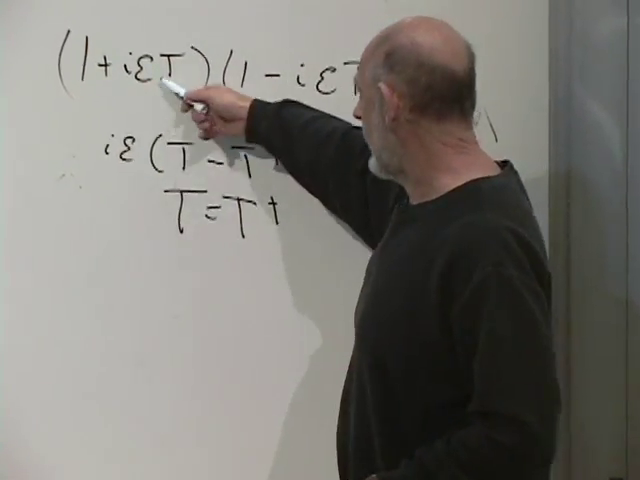
\includegraphics[width=0.62\textwidth]{lecture_04_figure_03.png}
\caption{Cálculo de la unitariedad cerca de la identidad, que termina en \(T=T^\dagger\).}
\lectureframe{00:23:28}
\end{figure}

Hay tres generadores linealmente independientes para las rotaciones espaciales, porque hay tres ejes infinitesimales independientes. Una rotación pequeña en una dirección arbitraria se construye mediante rotaciones pequeñas alrededor de \(x\), \(y\) y \(z\). Los generadores correspondientes son los operadores de momento angular \(J_x,J_y,J_z\). Sus conmutadores codifican la no conmutatividad de las rotaciones:
\begin{equation}
[J_i,J_j]=i\epsilon_{ijk}J_k.
\label{eq:l4-angular-momentum-algebra}
\end{equation}
Las rotaciones infinitesimales repetidas construyen entonces una rotación finita.

Hemos usado la unitariedad, pero todavía no la condición de determinante uno. Para cualquier matriz pequeña \(m\),
\begin{equation}
\det(\boldsymbol 1+\epsilon m)
=1+\epsilon\,\operatorname{tr}m+O(\epsilon^2).
\label{eq:l4-det-expansion}
\end{equation}

\begin{figure}[htbp]
\centering
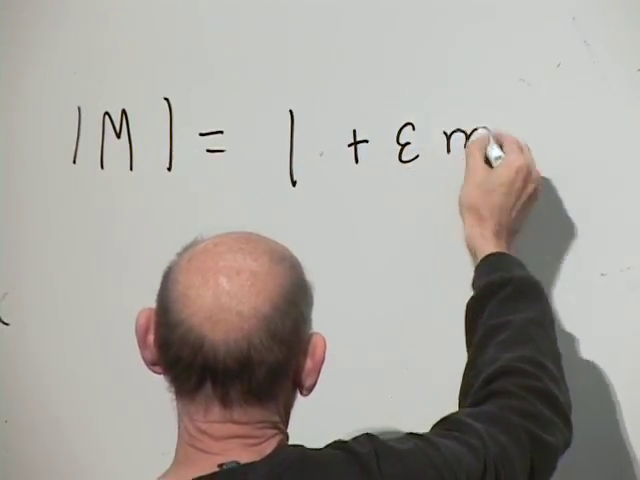
\includegraphics[width=0.62\textwidth]{lecture_04_figure_02.png}
\caption{Desarrollo del determinante a primer orden, tal como aparece al inicio en la pizarra.}
\lectureframe{00:21:51}
\end{figure}

Al aplicar la ecuación~\eqref{eq:l4-det-expansion} a la ecuación~\eqref{eq:l4-infinitesimal-u},
\begin{equation}
\det U
=1+i\epsilon\,\operatorname{tr}T+O(\epsilon^2).
\end{equation}
Por tanto, la condición de unitariedad especial exige que
\begin{equation}
\operatorname{tr}T=0.
\label{eq:l4-traceless-generator}
\end{equation}
Los generadores de \(SU(2)\) son precisamente las matrices hermíticas sin traza \(2\times2\). Ese espacio vectorial tiene dimensión tres. Las matrices de Pauli proporcionan una base estándar:
\begin{equation}
\begin{aligned}
\sigma_x&=
\begin{pmatrix}0&1\\1&0\end{pmatrix},
&
\sigma_y&=
\begin{pmatrix}0&-i\\i&0\end{pmatrix},
\\[0.4em]
\sigma_z&=
\begin{pmatrix}1&0\\0&-1\end{pmatrix}.
\end{aligned}
\end{equation}
Para una representación de espín un medio se puede tomar \(J_i=\sigma_i/2\), de modo que una rotación finita de ángulo \(\theta\) alrededor de \(\hat{\boldsymbol n}\) es
\begin{equation}
U(\hat{\boldsymbol n},\theta)
=\exp\!\left(-i\theta\,
\hat{\boldsymbol n}\cdot\boldsymbol\sigma/2\right).
\end{equation}
\editorialnote{La exponencial finita es la forma estándar de completar la discusión de los generadores infinitesimales. La fuente hace hincapié en las rotaciones pequeñas repetidas, en vez de escribir esta fórmula explícitamente.}

\begin{classroomqa}
\audiencequestion{¿Así que hay tres matrices hermíticas sin traza independientes \(2\times2\)?
\lecturetimestamp{00:24:07}}
\lecturerresponse{Sí. Son las tres matrices de Pauli. Para las matrices unitarias especiales \(3\times3\), el recuento correspondiente es ocho, y las ocho matrices de Gell-Mann forman una base convencional.}
\end{classroomqa}

\begin{classroomqa}
\audiencequestion{¿Ese ocho es el mismo ``ocho'' de la vía óctuple y los ocho gluones?
\lecturetimestamp{00:24:43}}
\lecturerresponse{Las matemáticas corresponden al mismo tipo de \(SU(3)\) teoría de representaciones, pero hay que especificar qué simetría \(SU(3)\) actúa. La simetría de sabor de la vía óctuple histórica no es el color \(SU(3)\). Los ocho gluones pertenecen a la representación adjunta del color \(SU(3)\).}
\end{classroomqa}

\section{De SU(2) al color SU(3)}

Ahora pasemos de matrices \(2\times2\) a matrices \(3\times3\). Una matriz compleja \(3\times3\) general tiene nueve elementos complejos, es decir, dieciocho parámetros reales. La condición \(U^\dagger U=\boldsymbol 1\) aporta nueve restricciones reales, y \(\det U=1\) impone una más. Por tanto,
\begin{equation}
18-9-1=8.
\end{equation}
Hay ocho direcciones infinitesimales independientes y ocho generadores hermíticos sin traza. A diferencia de \(SU(2)\), este grupo no es el grupo de rotaciones del espacio tridimensional ordinario. Es una simetría interna que actúa sobre el color.

Antes de asignar esas representaciones a los quarks, recordemos cómo surgen las representaciones compuestas. Pongamos juntos dos sistemas de espín un medio e ignoremos su movimiento orbital. Hay cuatro estados producto, pero una rotación no mezcla los cuatro de forma irreducible. Tres combinaciones se transforman como espín uno:
\begin{align}
\ket{1,1}&=\ket{\uparrow\uparrow},\\
\ket{1,0}&=\frac{1}{\sqrt2}
(\ket{\uparrow\downarrow}+\ket{\downarrow\uparrow}),\\
\ket{1,-1}&=\ket{\downarrow\downarrow},
\end{align}
mientras que la cuarta se transforma como espín cero:
\begin{equation}
\ket{0,0}=\frac{1}{\sqrt2}
(\ket{\uparrow\downarrow}-\ket{\downarrow\uparrow}).
\end{equation}
Así pues,
\begin{equation}
\boldsymbol 2\otimes\boldsymbol 2
=\boldsymbol 3\oplus\boldsymbol 1.
\label{eq:l4-two-spin-decomposition}
\end{equation}
Los estados alineados son los miembros \(m=\pm1\) del triplete; el estado simétrico de proyección cero lo completa, y la combinación antisimétrica es el singlete. Esta es la lógica general que subyace a la suma de momentos angulares y a la combinación de representaciones de color.

La misma distinción entre singlete--triplete aparece siempre que se acoplan dos grados de libertad de espín 1/2. En el hidrógeno atómico, los espines del electrón y del protón forman estados hiperfinos singlete y triplete. El ortohidrógeno y el parahidrógeno emplean la misma teoría de representaciones para los espines nucleares de los dos protones en una molécula de \(H_2\).\editorialnote{La fuente emplea ``ortohidrógeno y parahidrógeno'' al referirse a los espines protónicos--electrónicos de un átomo de hidrógeno. La descomposición matemática es correcta; aquí se distinguen los nombres moleculares y atómicos por precisión.}

\subsection{El triplete y el antitriplete}

Un quark tiene tres amplitudes de color. En una base elegida, escribamos
\begin{equation}
q=
\begin{pmatrix}
q_r\\q_g\\q_b
\end{pmatrix},
\qquad
q'=Uq,
\qquad U\in SU(3).
\label{eq:l4-quark-triplet}
\end{equation}
Las tres entradas pueden ser amplitudes de estado de un quark o tres operadores de campo que crean quarks rojos, verdes y azules. El grupo mezcla las tres componentes. Tras una transformación de color, un estado que inicialmente era rojo se convierte en general en una superposición de rojo, verde y azul. Esta representación fundamental tridimensional se llama \(\boldsymbol 3\).

Para un antiquark, el grupo actúa mediante la conjugada compleja de la representación del quark. Al tomar la conjugada compleja de la ecuación~\eqref{eq:l4-quark-triplet} se obtiene
\begin{equation}
\bar q'=U^*\bar q.
\end{equation}
Esta representación se denota \(\bar{\boldsymbol 3}\). La analogía con \(U(1)\) es inmediata: si un campo electrónico adquiere \(e^{i\theta}\), un campo de positrones adquiere \(e^{-i\theta}\). Las transformaciones de color de quarks y antiquarks constituyen la versión no abeliana de ese emparejamiento por conjugación.

Cerca de la identidad, si
\begin{equation}
U=\boldsymbol 1+i\epsilon T,
\end{equation}
entonces
\begin{equation}
U^*=\boldsymbol 1-i\epsilon T^*.
\end{equation}
Así pues, los generadores del antitriplete son \(-T^*\): los conjugados con el signo opuesto. Este es el sentido preciso en que los antiquarks tienen cargas de color opuestas.

\begin{classroomqa}
\audiencequestion{¿Qué ocurre con la representación conjugada compleja en el caso \(SU(2)\)?
\lecturetimestamp{00:36:19}}
\lecturerresponse{El doblete \(SU(2)\) es un caso especial: su conjugada compleja es equivalente al doblete original tras un cambio de base fijo que involucra el tensor épsilon antisimétrico. Para \(SU(3)\), en cambio, \(\boldsymbol 3\) y \(\bar{\boldsymbol 3}\) son representaciones genuinamente no equivalentes.}
\end{classroomqa}
\editorialnote{El término matemáticamente preciso para la representación fundamental de \(SU(2)\) es seudorreal, no real. La respuesta conserva la distinción que pretendía establecer la fuente y corrige la terminología.}

\section{Combinación de representaciones de color}

El símbolo \(\otimes\) no significa la multiplicación ordinaria de los números escritos junto a él. Significa que se combinan dos espacios de estados. El espacio producto tensorial resultante se reorganiza después en componentes que no se mezclan entre sí bajo la acción del grupo.

\subsection{Dos quarks: \texorpdfstring{\(\boldsymbol 3\otimes\boldsymbol 3\)}{3 x 3}}

Dos quarks tienen nueve estados de base de color: rojo--rojo, rojo--verde, rojo--azul y los seis pares ordenados restantes. Organicemos los dos índices de color en una parte simétrica y otra antisimétrica. La parte simétrica tiene seis componentes independientes; la antisimétrica tiene tres. Bajo \(SU(3)\),
\begin{equation}
\boldsymbol 3\otimes\boldsymbol 3
=\boldsymbol 6\oplus\bar{\boldsymbol 3}.
\label{eq:l4-three-times-three}
\end{equation}

\begin{figure}[htbp]
\centering
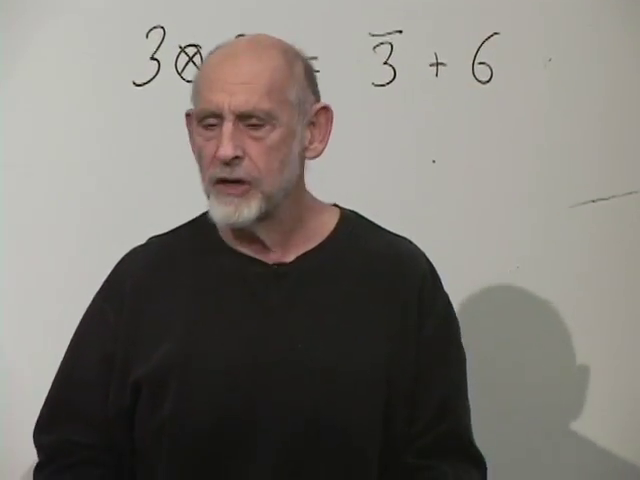
\includegraphics[width=0.68\textwidth]{lecture_04_figure_04.png}
\caption{Descomposición del producto de dos quarks en un antitriplete y un sextete.}
\lectureframe{00:39:33}
\end{figure}

El antitriplete se puede representar explícitamente contrayendo dos índices de quark con el tensor épsilon invariante:
\begin{equation}
(qq)^k_{\bar 3}
=\frac{1}{\sqrt2}\epsilon^{kij}q_iq_j.
\end{equation}
Este objeto tiene tres componentes y se transforma como un antiquark. Las seis combinaciones simétricas forman el sextete. No se afirma que dos quarks se conviertan dinámicamente en un antiquark, sino que un sector de su función de onda de color sigue la misma ley de transformación que un antiquark.

\subsection{Un quark y un antiquark: \texorpdfstring{\(\boldsymbol 3\otimes\bar{\boldsymbol 3}\)}{3 x anti-3}}

Un estado de color quark--antiquark se puede considerar una matriz \(3\times3\) \(M_i{}^j=q_i\bar q^j\). Toda matriz de este tipo se descompone de manera única en su parte de traza y su parte sin traza:
\begin{equation}
M=\frac{\operatorname{tr}M}{3}\boldsymbol 1
+\left(M-\frac{\operatorname{tr}M}{3}\boldsymbol 1\right).
\end{equation}
La traza es una única componente invariante, y la parte sin traza tiene ocho componentes. Por tanto,
\begin{equation}
\boldsymbol 3\otimes\bar{\boldsymbol 3}
=\boldsymbol 1\oplus\boldsymbol 8.
\label{eq:l4-three-times-threebar}
\end{equation}
El singlete, salvo por la normalización, es
\begin{equation}
\ket{1}_{q\bar q}
=\frac{1}{\sqrt3}
(\ket{r\bar r}+\ket{g\bar g}+\ket{b\bar b}).
\end{equation}
No puede rotar hacia ningún otro estado porque es invariante. Las otras ocho combinaciones lineales se mezclan entre sí. Constituyen la representación adjunta, la misma representación según la cual se transforman los ocho generadores.

\subsection{Tres quarks}

Combinemos un tercer quark con la ecuación~\eqref{eq:l4-three-times-three}. La rama del antitriplete da
\begin{equation}
\bar{\boldsymbol 3}\otimes\boldsymbol 3
=\boldsymbol 1\oplus\boldsymbol 8,
\end{equation}
Así, el producto de tres quarks contiene un singlete. En su forma completa,
\begin{equation}
\boldsymbol 3\otimes\boldsymbol 3\otimes\boldsymbol 3
=\boldsymbol 1\oplus\boldsymbol 8\oplus\boldsymbol 8
\oplus\boldsymbol{10}.
\label{eq:l4-three-quark-full}
\end{equation}
El singlete de color es la combinación totalmente antisimétrica rojo--verde--azul:
\begin{equation}
\ket{1}_{qqq}
=\frac{1}{\sqrt6}\epsilon^{ijk}\ket{q_iq_jq_k}.
\label{eq:l4-baryon-singlet}
\end{equation}
Como \(\epsilon^{ijk}\) se anula cuando dos índices coinciden, cada término no nulo contiene un quark rojo, uno verde y uno azul, con signos alternos al intercambiarlos.

\begin{classroomqa}
\audiencequestion{¿Son simplemente improbables las combinaciones no singlete, de modo que podemos ignorar sus probabilidades?
\lecturetimestamp{00:46:02}}
\lecturerresponse{No. El problema es la energía, no que la probabilidad sea pequeña. Un estado no singlete aislado tendría un campo de color que se extendería hasta distancias arbitrariamente grandes y, en el régimen de confinamiento, requeriría una energía ilimitada. Más adelante desarrollaremos la dinámica que sustenta esta afirmación.}
\end{classroomqa}

\subsection{El octeto de gluones}

El campo de gluones se transforma como el octeto de la ecuación~\eqref{eq:l4-three-times-threebar}. Respecto del color, lleva un índice de triplete y uno de antitriplete, y se elimina la traza singlete. Esquemáticamente,
\begin{equation}
q\sim\boldsymbol 3,
\qquad
\bar q\sim\bar{\boldsymbol 3},
\qquad
G\sim\boldsymbol 8.
\end{equation}
Estos símbolos indican leyes de transformación; las partículas no son literalmente iguales a los números tres y ocho.

La novena combinación de color quark--antiquark, proporcional a la identidad, es un singlete y no se mezcla con el octeto. Por tanto, es matemáticamente coherente omitirla: un campo gauge \(SU(3)\) no tiene traza y tiene ocho componentes, frente a las nueve de un campo gauge \(U(3)\).

\begin{classroomqa}
\audiencequestion{¿Por qué la naturaleza omite el gluón singlete adicional?
\lecturetimestamp{00:49:00}}
\lecturerresponse{La respuesta inmediata desde la teoría de grupos es que el singlete constituye un sector invariante separado, de modo que el octeto se cierra de manera consistente sin él. Aquí no se deriva la razón más profunda para elegir \(SU(3)\) en lugar de \(U(3)\); forma parte de la estructura gauge que se infiere de la fenomenología de la QCD.}
\end{classroomqa}

\section{Los singletes de color como hadrones}

Las partículas libres de masa finita de la interacción fuerte son singletes de color. Esto no significa que los quarks o los gluones no sean reales; significa que no aparecen como partículas asintóticas aisladas. Los patrones elementales para formar singletes son
\begin{equation}
qqq,
\qquad
q\bar q,
\qquad
GG\ \text{and higher gluonic products}.
\end{equation}
Dan lugar, respectivamente, a bariones, mesones y glueballs. Los productos de varios objetos ya neutros en color también son neutros, por supuesto, así que con estos componentes se pueden construir estados multihadrónicos más complejos.

\begin{classroomqa}
\audiencequestion{¿Cómo se llaman los singletes de tres quarks y de quark--antiquark, y también pueden los gluones formar singletes?
\lecturetimestamp{00:51:38}}
\lecturerresponse{Un singlete de tres quarks es un barión; un singlete de quark--antiquark es un mesón. Los gluones también pueden combinarse en singletes de color. Los estados más sencillos de este tipo que participan en la interacción fuerte se llaman glueballs, y pueden intervenir más de dos gluones.}
\end{classroomqa}

Tres quarks de espín un medio siempre se combinan para dar un espín total semientero, aunque el momento angular orbital puede cambiar cuál de ellos se obtiene. Los mesones de quark--antiquark tienen espín entero. Los glueballs puramente gluónicos también tienen espín entero.

La primera afirmación de la pizarra sobre dos gluones es solo un recuento:
\begin{equation}
8\times8=1+63.
\end{equation}
Hay sesenta y cuatro estados de color en total; una combinación es un singlete y los sesenta y tres restantes pertenecen a sectores no singlete.

\begin{figure}[htbp]
\centering
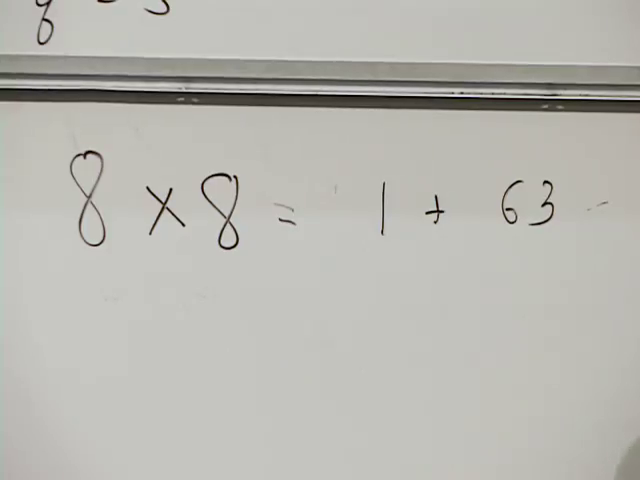
\includegraphics[width=0.68\textwidth]{lecture_04_figure_05.png}
\caption{Recuento de estados de dos gluones en la pizarra: un singlete entre sesenta y cuatro estados.}
\lectureframe{00:53:44}
\end{figure}

La descomposición irreducible completa es
\begin{equation}
\boldsymbol 8\otimes\boldsymbol 8
=\boldsymbol 1\oplus\boldsymbol 8_S\oplus\boldsymbol 8_A
\oplus\boldsymbol{10}\oplus\overline{\boldsymbol{10}}
\oplus\boldsymbol{27}.
\label{eq:l4-eight-times-eight}
\end{equation}
Las dimensiones suman correctamente:
\begin{equation}
1+8+8+10+10+27=64.
\end{equation}
Los dos octetos son subespacios invariantes distintos, uno simétrico y otro antisimétrico bajo el intercambio de los dos factores adjuntos. El singlete es el canal de color de dos gluones a partir del cual se puede formar un estado glueball.
\editorialnote{La pizarra da primero solo \(8\times8=1+63\). El intercambio posterior en clase proporciona las dimensiones irreducibles indicadas; aquí se restablecen las barras y las etiquetas de simetría con la notación estándar de \(SU(3)\).}

\subsection{Por qué las cargas eléctricas observables son enteras}

Las cargas de los quarks son de dos tipos:
\begin{equation}
Q_{\mathrm{up\text{-}like}}=+\frac23,
\qquad
Q_{\mathrm{down\text{-}like}}=-\frac13.
\end{equation}
Por tanto, tres quarks tienen una carga total entera: \(-1,0,+1,\text{ or }+2\), según cuántos sean del tipo up. Del mismo modo, un quark y un antiquark tienen carga \(0\) o \(\pm1\). Los gluones no tienen carga eléctrica. Así, los singletes de color básicos construidos con las representaciones de quarks observadas tienen carga eléctrica entera, aunque sus constituyentes tengan cargas fraccionarias.

\begin{classroomqa}
\audiencequestion{¿Cuál es la carga eléctrica del quark extraño?
\lecturetimestamp{00:56:08}}
\lecturerresponse{Es del tipo down, así que su carga es \(-1/3\). Las tres familias repiten el mismo patrón de cargas: \((u,d)\), \((c,s)\) y \((t,b)\), con cargas \(+2/3\) y \(-1/3\) en cada pareja.}
\end{classroomqa}

La condición de singlete de color y la carga eléctrica entera están estrechamente relacionadas para este contenido de partículas, pero no son afirmaciones matemáticas idénticas. La integridad también depende de las asignaciones concretas de carga eléctrica del modelo estándar que acabamos de escribir.

\begin{classroomqa}
\audiencequestion{¿Es un estado entrelazado un singlete de color, y tiene eso la misma importancia que una pareja entrelazada en un experimento de Bell?
\lecturetimestamp{00:56:58}}
\lecturerresponse{La función de onda del singlete de color sí está entrelazada: es una superposición coherente, no un producto de colores definidos por separado. En principio, sus constituyentes se pueden separar, pero el confinamiento hace que esa separación sea cada vez más costosa y, finalmente, produzca nuevos hadrones. Por eso no es un sistema práctico para una manipulación al estilo de Bell, aunque el estado esté entrelazado.}
\end{classroomqa}

\section{Qué significan las ecuaciones de producto tensorial}

En este punto, las tablas de multiplicación merecen una explicación más concreta. Sean \(\psi_i\) y \(\phi_j\) operadores que crean dos objetos de espín un medio; pueden describir dos especies, como un electrón y un protón, o dos copias de la misma especie cuando se tiene en cuenta la estadística apropiada. Cada índice toma dos valores. Los cuatro productos
\begin{equation}
\psi_\uparrow\phi_\uparrow,
\quad
\psi_\uparrow\phi_\downarrow,
\quad
\psi_\downarrow\phi_\uparrow,
\quad
\psi_\downarrow\phi_\downarrow
\end{equation}
generan el espacio producto tensorial.

Si un elemento del grupo actúa como \(U\) sobre cada factor, actúa como \(U\otimes U\) sobre el producto. En componentes,
\begin{equation}
\psi_i\phi_j
\longmapsto
U_i{}^kU_j{}^\ell\psi_k\phi_\ell.
\label{eq:l4-product-action}
\end{equation}
Esta es una representación tetradimensional, pero reducible. La combinación antisimétrica
\begin{equation}
\frac{1}{\sqrt2}
(\psi_\uparrow\phi_\downarrow
-\psi_\downarrow\phi_\uparrow)
\end{equation}
se transforma en sí misma, mientras que las tres combinaciones simétricas se transforman entre sí. En la base adaptada a esas combinaciones, todas las matrices de la representación producto adoptan una forma diagonal por bloques:
\begin{equation}
D_{2\otimes2}(g)
\sim
\begin{pmatrix}
1&0\\
0&D_3(g)
\end{pmatrix}.
\label{eq:l4-spin-block-diagonal}
\end{equation}

\begin{classroomqa}
\audiencequestion{¿Qué operación representa una ecuación como \(\boldsymbol 3\otimes\boldsymbol 3=\bar{\boldsymbol 3}\oplus\boldsymbol 6\)?
\lecturetimestamp{00:57:51}}
\lecturerresponse{El miembro izquierdo forma el espacio de estados compuesto. El grupo actúa sobre ambos factores y, por tanto, mezcla los estados de la base producto. El miembro derecho indica que un cambio de base separa esos estados en conjuntos invariantes: tres combinaciones antisimétricas que se transforman como un antitriplete y seis combinaciones simétricas que se transforman como un sextete. El signo más indica una suma directa de alternativas, no una suma numérica ordinaria.}
\end{classroomqa}

\begin{classroomqa}
\audiencequestion{¿Cómo sabemos que los nueve estados se descomponen como \(3+6\), o como \(1+8\), en lugar de, por ejemplo, como \(2+7\)?
\lecturetimestamp{01:04:39}}
\lecturerresponse{El recuento de dimensiones por sí solo no permite decidir la descomposición. Hay que saber qué representaciones irreducibles contiene \(SU(3)\) y construir subespacios invariantes, por ejemplo, simetrizando o antisimetrizando índices, o separando las partes con traza y sin traza. Una clasificación completa requiere más teoría de grupos; aquí solo usamos las representaciones necesarias para los quarks y los gluones.}
\end{classroomqa}

El tensor épsilon invariante hace transparente la construcción del singlete. Para \(SU(2)\),
\begin{equation}
\epsilon_{ij}U^i{}_kU^j{}_\ell
=(\det U)\epsilon_{k\ell}
=\epsilon_{k\ell}.
\end{equation}
Por tanto, \(\epsilon_{ij}\psi^i\phi^j\) es invariante. Para \(SU(3)\), la versión con tres índices da
\begin{equation}
\epsilon_{ijk}U^i{}_aU^j{}_bU^k{}_c
=(\det U)\epsilon_{abc}
=\epsilon_{abc},
\end{equation}
lo que demuestra la invariancia del estado de tres quarks de la ecuación~\eqref{eq:l4-baryon-singlet}.

\begin{classroomqa}
\audiencequestion{¿Se puede mostrar explícitamente por qué el singlete no se transforma?
\lecturetimestamp{01:07:18}}
\lecturerresponse{Sí. Contraigamos todos los índices fundamentales con el tensor épsilon totalmente antisimétrico. Bajo la transformación, el producto de matrices multiplica épsilon por \(\det U\). Para una matriz unitaria especial, ese determinante es uno, así que el estado contraído no cambia. En \(SU(2)\) esto demuestra la invariancia del singlete de dos espines; en \(SU(3)\) demuestra la del singlete de tres quarks rojo--verde--azul.}
\end{classroomqa}

\begin{classroomqa}
\audiencequestion{¿Cuál es la descomposición completa de dos octetos de gluones?
\lecturetimestamp{01:09:24}}
\lecturerresponse{Es la descomposición de la ecuación~\eqref{eq:l4-eight-times-eight}: un singlete, dos octetos, un decuplete, un antidecuplete y una representación de dimensión veintisiete. Hay exactamente una combinación de singlete de color de los dos índices de octeto.}
\end{classroomqa}

\begin{classroomqa}
\audiencequestion{¿Cuál es la descomposición completa correspondiente para tres quarks?
\lecturetimestamp{01:11:51}}
\lecturerresponse{La respuesta esencial desde el punto de vista físico es que contiene un singlete. Al completar el recuento se obtiene la ecuación~\eqref{eq:l4-three-quark-full}: un singlete, dos octetos y un decuplete, para un total de \(1+8+8+10=27\) estados.\editorialnote{Durante el intercambio, el profesor no recuerda la descomposición completa de \(3\otimes3\otimes3\). Aquí se proporciona explícitamente la descomposición estándar y se señala que no formó parte de la respuesta oral.}}
\end{classroomqa}

La misma idea se extiende al espacio de dos gluones. En la base producto ingenua,
\(SU(3)\) actúa mediante matrices \(64\times64\). En una base adaptada a las componentes irreducibles, esas matrices son diagonales por bloques,
\begin{equation}
\begin{aligned}
D_{8\otimes8}(g)
&\sim
\operatorname{diag}\bigl(
1,D_{8_S}(g),D_{8_A}(g),
\\
&\hspace{4.8em}
D_{10}(g),D_{\overline{10}}(g),D_{27}(g)
\bigr).
\end{aligned}
\end{equation}
Ningún bloque se mezcla con otro, aunque los estados de cada bloque sí se mezclan entre sí.

\begin{classroomqa}
\audiencequestion{¿La descomposición en productos tensoriales es simplemente un cambio a una base en la que la matriz grande de la representación queda diagonal por bloques?
\lecturetimestamp{01:12:02}}
\lecturerresponse{Exactamente. Para dos espines, la matriz de dimensión cuatro se convierte en un bloque singlete unidimensional y otro triplete de dimensión tres. Para dos gluones, la matriz de dimensión sesenta y cuatro se convierte en bloques de dimensiones \(1,8,8,10,10,\text{ and }27\). Cada bloque es cerrado bajo toda transformación del grupo.}
\end{classroomqa}

\begin{classroomqa}
\audiencequestion{¿Hay un nombre para una de esas partes cerradas dentro del espacio producto tensorial completo?
\lecturetimestamp{01:14:55}}
\lecturerresponse{Es un subespacio invariante que lleva una subrepresentación. Cuando no puede descomponerse más, lleva una representación irreducible, o irrep. El producto tensorial completo es la suma directa de esas componentes irreducibles.\editorialnote{En la fuente, el término solicitado queda sin resolver en el aula. La respuesta aporta la terminología estándar de la teoría de representaciones.}}
\end{classroomqa}

\begin{classroomqa}
\audiencequestion{Cuando se dice que los decupletes no singletes y otras representaciones no existen, ¿significa que deben ignorarse por completo?
\lecturetimestamp{01:15:36}}
\lecturerresponse{Son sectores de color legítimos e importan en los cálculos intermedios, pero no aparecen como partículas aisladas de energía finita en el laboratorio. Es el confinamiento, y no un fallo de la teoría de representaciones, lo que impide que se conviertan en estados asintóticos libres.}
\end{classroomqa}

\section{De la idea del color de Nambu al confinamiento}

La idea del color precede a la formulación definitiva de la QCD. Ya a principios de los años 1960, Yoichiro Nambu comprendió que un número cuántico oculto con tres valores podía resolver un problema sorprendente: los quarks tienen carga eléctrica fraccionaria, pero no se observan partículas libres con carga fraccionaria. Si se obliga a que los estados físicos sean singletes de color, los quarks aparecen en las combinaciones de carga entera descritas anteriormente. Queda la cuestión dinámica: ¿qué fuerzas hacen que todos los estados libres de energía finita sean singletes?

Empecemos con la analogía electromagnética. Una carga y otra de signo opuesto se atraen. Al acercarlas, disminuye la energía; juntar cargas del mismo signo requiere trabajo. El propio campo almacena energía positiva,
\begin{equation}
E_{\mathrm{field}}
=\frac12\int d^3x\,\boldsymbol E^2
\end{equation}
en unidades electrostáticas simples. Una carga neta deja un campo que se extiende mucho más allá del sistema, mientras que un par neutro estrechamente ligado solo tiene un campo dipolar de corto alcance. Por tanto, la neutralización elimina la energía del campo exterior.

Imaginemos que aumentamos enormemente el acoplamiento electromagnético. La penalización energética del campo por tener carga neta sería tan grande que los objetos de baja energía serían abrumadoramente neutros, y extraer un constituyente cargado podría resultar prohibitivamente costoso. Nambu trasladó esta intuición al color: las ocho cargas de color son fuentes de ocho campos gluónicos, así que una energía grande del campo de color podría impedir la existencia de estados no singletes aislados.

Esa intuición es esencialmente correcta, pero la QCD presenta una característica nueva decisiva. El fotón no tiene carga eléctrica, mientras que el gluón tiene carga de color. El fotón no es fuente del campo electromagnético clásico, y las ecuaciones de Maxwell son lineales: dos ondas electromagnéticas se superponen y atraviesan una a otra. El gluón se transforma según el octete de color, así que los gluones son fuentes e interactúan con otros gluones. Incluso distintas partes de un mismo campo gluónico interactúan entre sí. Por tanto, el campo de gauge no abeliano es no lineal.

\subsection{Tubos de flujo y potencial lineal}

A grandes distancias, la auto-interacción de los gluones impide que el flujo de color se disperse como un campo dipolar eléctrico ordinario. El flujo queda confinado en un tubo que une un quark con un antiquark. La intensidad del campo y el área de la sección transversal de un tubo largo son aproximadamente constantes, por lo que el tubo almacena una energía aproximadamente constante por unidad de longitud. Si \(\sigma\) denota esta tensión de cuerda, entonces
\begin{equation}
V(R)\simeq\sigma R+\text{constant}
\qquad (R\ \text{large}).
\label{eq:l4-linear-potential}
\end{equation}

\begin{figure}[htbp]
\centering
\includegraphics[width=0.78\textwidth]{lecture_04_figure_06.png}
\caption{Flujo de color agrupado en un tubo largo entre un quark y un antiquark.}
\lectureframe{01:31:35}
\end{figure}

Esto es más intenso que el potencial de Coulomb, cuya magnitud disminuye como \(1/R\).
Al separar más las fuentes de color, la fuerza no se debilita indefinidamente: el tubo se alarga y sigue acumulando energía. Una carga de color aislada en un volumen infinito requeriría un tubo sin fin y, por tanto, energía ilimitada. Este es el significado operativo de afirmar que solo los singletes de color tienen estados asintóticos de energía finita.
\editorialnote{La notación de la tensión de cuerda y el potencial explícito a grandes distancias cuantifican la afirmación de la fuente de que un tubo de flujo uniforme tiene una energía uniforme por unidad de longitud.}

\subsection{Ruptura de cuerdas y chorros}

Supongamos que una colisión de alta energía golpea un quark dentro de un mesón. El quark empieza a alejarse, pero el tubo de flujo se estira detrás de él. Puede perder energía cinética y ser arrastrado de vuelta. Con más frecuencia, cuando la energía almacenada en el campo es suficientemente grande, el vacío produce un nuevo par quark--antiquark. El nuevo antiquark termina el flujo unido al quark que escapa, mientras que el nuevo quark termina el flujo unido al antiquark original. Un singlete estirado se convierte en dos singletes más cortos,
\begin{equation}
(q\bar q)_{\mathrm{stretched}}
\longrightarrow
(q\bar q)+(q\bar q).
\label{eq:l4-string-breaking}
\end{equation}

\begin{figure}[htbp]
\centering
\includegraphics[width=0.78\textwidth]{lecture_04_figure_07.png}
\caption{La creación de pares rompe un tubo de flujo estirado en dos tubos singletes de color.}
\lectureframe{01:34:52}
\end{figure}

\begin{classroomqa}
\audiencequestion{Si un quark golpeado tiene suficiente energía para seguir estirando el tubo, ¿qué puede ocurrir además de que lo arrastren de vuelta?
\lecturetimestamp{01:33:50}}
\lecturerresponse{El tubo puede romperse mediante la creación de un par quark--antiquark. Su energía se convierte en la masa y la energía cinética del nuevo par. Los extremos se reconectan formando dos singletes, de modo que el proceso crea mesones adicionales en lugar de un quark aislado.}
\end{classroomqa}

Si uno de esos partones todavía tiene un momento grande, el proceso se repite. El resultado es una cascada de hadrones singletes de color, colimados alrededor de la dirección del partón original: un chorro. Esta conversión de quarks y gluones energéticos en hadrones se denomina hadronización. El objeto coloreado que inicia el proceso se infiere a partir del chorro; nunca se observa por sí solo.

\begin{classroomqa}
\audiencequestion{¿La ruptura de cuerdas produce únicamente mesones o también pueden aparecer otros hadrones en el chorro?
\lecturetimestamp{01:35:20}}
\lecturerresponse{Desde luego, también pueden aparecer otros hadrones. El único requisito de color es que los objetos observables finales sean singletes. Los mesones son la imagen más sencilla para una ruptura, pero también pueden producirse bariones, antibariones y combinaciones singletes más complejas.}
\end{classroomqa}

Tres quarks pueden terminar sus líneas de flujo en una unión singlete de color. La imagen de tres ramificaciones es la contraparte dinámica del tensor epsilon antisimétrico de la ecuación~\eqref{eq:l4-baryon-singlet}: no escapa flujo neto de color del barión completo.

\begin{figure}[htbp]
\centering
\includegraphics[width=0.72\textwidth]{lecture_04_figure_08.png}
\caption{Una unión de flujo de color con tres ramificaciones para un barión, debajo del esquema de ruptura de la cuerda del mesón.}
\lectureframe{01:36:12}
\end{figure}

\section{Campos de gauge, cargas conservadas y modelo estándar}

En el nivel actual, podemos reconocer una teoría de gauge como una teoría en la que una carga conservada es fuente de un campo análogo al del fotón. La carga eléctrica es fuente del campo electromagnético; las ocho cargas de color son fuentes de los ocho campos gluónicos. La formulación más profunda hace local la simetría e introduce una conexión que compara los estados internos en puntos vecinos del espacio-tiempo, pero esa construcción no hace falta para la explicación del confinamiento que desarrollamos aquí.
\editorialnote{La formulación mediante simetría local es el sentido más profundo y estándar de teoría de gauge al que alude la fuente, pero que deja deliberadamente para más adelante.}

La simetría, la carga conservada y el flujo están estrechamente relacionados. Si las líneas de campo solo pueden terminar en cargas, una fuente no puede desaparecer sin más mientras su flujo siga unido a algo. Tampoco puede desaparecer instantáneamente todo su campo distante, porque los cambios del campo se propagan causalmente. En su forma local, la misma física se expresa mediante una ecuación de continuidad,
\begin{equation}
\frac{\partial\rho}{\partial t}
+\boldsymbol\nabla\cdot\boldsymbol j=0,
\end{equation}
que establece que una carga solo puede salir de una región si fluye a través de su frontera. El argumento de las líneas de campo es la representación geométrica de esa ley local de conservación.

Ahora podemos situar este resultado dentro del modelo estándar. El color aporta los ocho generadores de \(SU(3)\) y sus ocho campos gluónicos. El sector abeliano aporta un generador y un campo de gauge. Otros tres generadores pertenecen a un \(SU(2)\) adicional, no al momento angular espacial ordinario. Antes de la ruptura de simetría, la estructura de gauge es
\begin{equation}
SU(3)_c\times SU(2)_L\times U(1)_Y,
\end{equation}
con \(8+3+1=12\) generadores. La siguiente tarea es comprender el sector electrodébil \(SU(2)\) y, después, el campo de Higgs y cómo aparecen el fotón observado, \(W^\pm\) y \(Z\).
\editorialnote{La fuente cuenta el fotón junto con los ocho gluones y describe el factor restante como \(SU(2)\times U(1)\). En el modelo estándar sin ruptura, el factor abeliano es la hipercarga \(U(1)_Y\); el fotón aparece solo después de la mezcla electrodébil.}

La cadena central está ahora completa. Los grupos abstractos actúan mediante representaciones; los generadores infinitesimales son las cargas conservadas; los quarks, antiquarks y gluones pertenecen a \(\boldsymbol 3\),
\(\bar{\boldsymbol 3}\) y \(\boldsymbol 8\), respectivamente; los productos tensoriales identifican los hadrones singletes; y el campo gluónico no lineal convierte la selección de singletes en el fenómeno físico del confinamiento.

\chapter{Campos gauge, escalas de interacción y corrientes débiles cargadas}

La electrodinámica cuántica y la cromodinámica cuántica parecen muy distintas en el laboratorio, pero ambas son teorías gauge. De hecho, casi todas las interacciones del modelo estándar se organizan de este modo. La palabra \emph{gauge} tiene un significado más profundo relacionado con la simetría local, pero podemos dejar de lado por ahora ese formalismo. De momento necesitamos una descripción física mínima: una teoría gauge contiene campos de tipo Maxwell, fuentes conservadas, transformaciones de simetría, bosones gauge y reglas para emitir y absorber esos bosones.

\section{La teoría de Maxwell como prototipo}

\subsection{Campos y potenciales}

El campo electromagnético tiene seis componentes: tres del campo eléctrico y tres del campo magnético. La misma información puede codificarse, con cierta redundancia, en un potencial de cuatro componentes
\begin{equation}
A_\mu=(A_0,\boldsymbol A),
\end{equation}
donde \(A_0\) es el potencial electrostático y \(\boldsymbol A\) es el potencial vectorial espacial. En el límite electrostático, el campo eléctrico se obtiene a partir del gradiente espacial:
\begin{equation}
\boldsymbol E=-\boldsymbol\nabla A_0,
\qquad
\boldsymbol F=q\boldsymbol E,
\end{equation}
mientras que el campo magnético es
\begin{equation}
\boldsymbol B=\boldsymbol\nabla\times\boldsymbol A.
\end{equation}
El signo de la primera ecuación depende de la definición estándar del potencial; en la explicación en la pizarra interesa sobre todo que los campos son derivadas de los potenciales.
\editorialnote{Para campos dependientes del tiempo, la relación completa es
\(\boldsymbol E=-\boldsymbol\nabla A_0-\partial_t\boldsymbol A\). Aquí, la clase trabaja deliberadamente con el caso electrostático más sencillo.}

\begin{figure}[htbp]
\centering
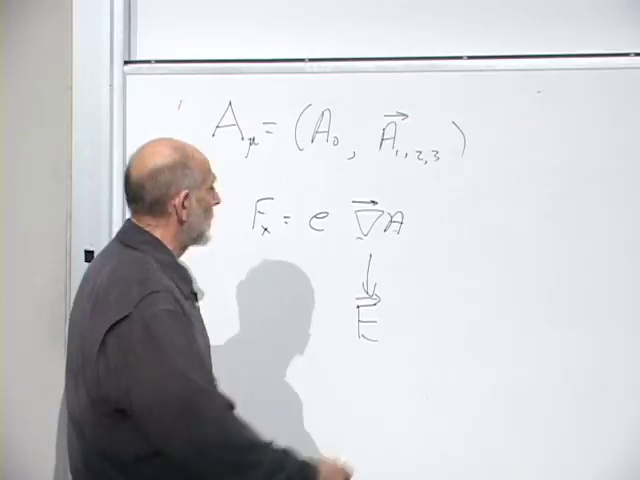
\includegraphics[width=0.62\textwidth]{lecture_05_figure_02.png}
\caption{El potencial electromagnético de cuatro componentes y su relación, mediante derivadas, con el campo.}
\lectureframe{00:03:33}
\end{figure}

Así pues, la electrodinámica admite dos descripciones equivalentes: una en términos de \(\boldsymbol E\) y \(\boldsymbol B\), y otra en términos de \(A_\mu\). Esta última solo tiene cuatro componentes explícitas porque distintos potenciales pueden describir los mismos campos físicos. Esa redundancia es el primer indicio del significado de la palabra gauge, aunque todavía no la usaremos de manera formal.

\subsection{Ondas y polarización}

Las ecuaciones de Maxwell admiten ondas. Consideremos una onda plana que se propaga en la dirección del vector unitario \(\hat{\boldsymbol k}\). En cada punto, los campos eléctrico y magnético son transversales:
\begin{equation}
\boldsymbol E\cdot\hat{\boldsymbol k}=0,
\qquad
\boldsymbol B\cdot\hat{\boldsymbol k}=0,
\qquad
\boldsymbol E\cdot\boldsymbol B=0.
\end{equation}
En unidades en las que \(c=1\), sus módulos son iguales:
\begin{equation}
|\boldsymbol E|=|\boldsymbol B|.
\end{equation}
En una onda polarizada linealmente, la dirección de \(\boldsymbol E\) especifica la polarización. Todo el patrón se propaga a la velocidad de la luz.

La cuantización cambia el lenguaje, pero no la estructura de la polarización. Un cuanto de la onda electromagnética es un fotón. Representar un fotón como un punto resulta inevitablemente engañoso, pero es útil imaginar que el punto lleva un pequeño indicador transversal que señala su polarización. Una lámina de cuarto de onda u otro elemento óptico puede rotar esa polarización. También puede imaginarse, solo de manera aproximada, que un campo de Coulomb estático surge de la emisión y absorción repetidas de fotones.

\subsection{Fuentes, flujo y conservación}

Las ondas electromagnéticas pueden propagarse por el espacio vacío, pero el campo también tiene fuentes: las cargas y corrientes eléctricas. Una carga puntual positiva produce un campo eléctrico radial saliente proporcional a \(1/r^2\). El número de líneas de campo que atraviesa cualquier esfera alrededor de la carga es independiente del radio de la esfera. Matemáticamente,
\begin{equation}
\oint_{S^2}\boldsymbol E\cdot d\boldsymbol S
=\frac{Q_{\mathrm{enc}}}{\epsilon_0},
\label{eq:l5-gauss}
\end{equation}
en unidades SI.

Esto es más que una manera práctica de calcular el campo. Las líneas del campo eléctrico solo pueden terminar en una carga. Si una carga aislada desapareciera sin más, su campo tendría que desaparecer en todas partes simultáneamente, en violación de la causalidad, o bien un frente de campo ausente tendría que propagarse hacia fuera, con líneas de campo que terminaran en el espacio vacío. Ninguna de las dos cosas está permitida. Por tanto, la geometría del flujo hace natural la conservación de la carga: las cargas pueden moverse y las cargas opuestas pueden aniquilarse, pero la carga neta no puede desaparecer localmente sin una corriente compensatoria.

La expresión local correspondiente es la ecuación de continuidad
\begin{equation}
\partial_t\rho+\boldsymbol\nabla\cdot\boldsymbol J=0.
\label{eq:l5-continuity}
\end{equation}
\editorialnote{~\eqref{eq:l5-continuity} es la forma matemática local estándar del argumento causal sobre el flujo expuesto verbalmente en la clase.}

\subsection{Definición operativa de teoría gauge}

Ya podemos enunciar el patrón operativo. Una teoría gauge tiene:
\begin{itemize}
\item campos de tipo eléctrico y magnético;
\item ondas que, cuando las interacciones son suficientemente débiles, se parecen a las ondas de luz;
\item fuentes análogas a la carga eléctrica;
\item una ley de Gauss que relaciona el flujo con esas fuentes;
\item una ley de conservación y una simetría asociada;
\item cuantos del campo, llamados bosones gauge; y
\item una constante de acoplamiento que controla la emisión y la absorción.
\end{itemize}
La fuente no tiene por qué ser la carga eléctrica. Como ejemplo deliberadamente no físico, imaginemos que se introduce una simetría gauge para el número bariónico. Los protones y los neutrones tienen ambos número bariónico \(+1\), así que se repelerían mediante una nueva fuerza de tipo Coulomb; un protón y un antiprotón se atraerían. Una teoría así es matemáticamente concebible, pero la naturaleza no presenta ningún campo gauge de largo alcance observado que esté acoplado al número bariónico. La conservación por sí sola no garantiza la existencia de una fuerza gauge.

La carga eléctrica sí va acompañada de una simetría. Para un campo de materia cargado,
\begin{equation}
\psi(x)\longmapsto e^{i\theta}\psi(x).
\label{eq:l5-u1}
\end{equation}
La simetría de fase y la conservación de la carga son dos aspectos de la misma estructura. Más adelante podremos hacer que \(\theta\) dependa del espacio-tiempo y ver por qué se necesita el potencial \(A_\mu\). Aquí basta la transformación global para identificar la carga conservada.

\section{La QCD como ejemplo no abeliano}

\subsection{Tripletes, antitripletes y la matriz de gluones}

En cromodinámica cuántica, un campo de quarks lleva un índice de color \(i\in\{r,g,b\}\) y se transforma en la representación fundamental de \(SU(3)\):
\begin{equation}
q'_i=U_{ij}q_j,
\qquad
U^\dagger U=\boldsymbol 1,
\qquad
\det U=1.
\label{eq:l5-q-transform}
\end{equation}
Esta es una rotación en un espacio de color complejo tridimensional, no una rotación del espacio de posiciones ordinario. A la representación de tres componentes también se la llama representación definitoria.

Los campos de antipartículas se representan mediante las variables complejas conjugadas. Al tomar el conjugado complejo de la ecuación~\eqref{eq:l5-q-transform} se obtiene
\begin{equation}
q_i^{\prime *}=U_{ij}^*q_j^*.
\label{eq:l5-antiquark-transform}
\end{equation}
Así pues, los quarks se transforman como \(\boldsymbol 3\), mientras que los antiquarks se transforman como \(\bar{\boldsymbol 3}\).

\begin{figure}[htbp]
\centering
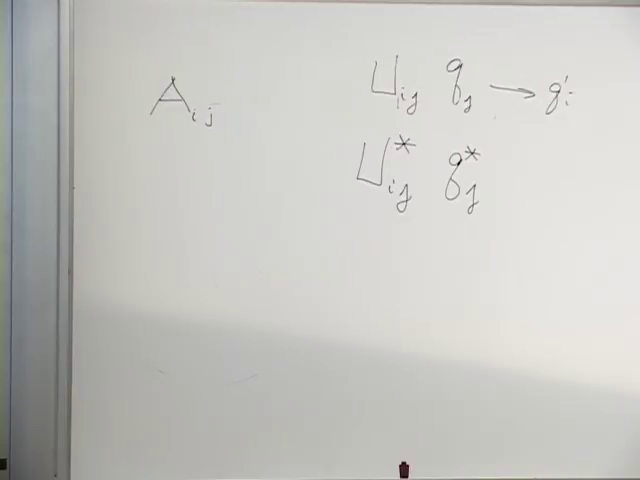
\includegraphics[width=0.62\textwidth]{lecture_05_figure_03.png}
\caption{La transformación fundamental y la transformación conjugada compleja del antitriplete.}
\lectureframe{00:18:47}
\end{figure}

\begin{classroomqa}\audiencequestion{¿Cuántas matrices \(U\) hay--, ¿siete, ocho o nueve?
\lecturetimestamp{00:19:37}}\lecturerresponse{Hay infinitos elementos del grupo \(U\). Lo que se cuenta es el número finito de generadores independientes: ocho para \(SU(3)\). Una matriz general \(3\times3\) tiene nueve posiciones matriciales, pero la unitariedad especial deja ocho direcciones continuas.}\end{classroomqa}

El campo de gluones puede escribirse como una matriz sin traza \(A_{ij}\). Un índice se transforma como el de un quark y el otro como el de un antiquark, de modo que su estructura de color es la de
\begin{equation}
\boldsymbol 3\otimes\bar{\boldsymbol 3}
=\boldsymbol 1\oplus\boldsymbol 8.
\end{equation}
La QCD conserva el octete sin traza,
\begin{equation}
A_{ii}=\operatorname{tr}A=0,
\end{equation}
y descarta el singlete. Por eso la QCD tiene ocho gluones y no nueve. En general, \(SU(N)\) tiene
\begin{equation}
N^2-1
\end{equation}
generadores y el mismo número de campos de bosones gauge.

El fotón es neutro bajo \(U(1)\) eléctrico: rotar la fase de un electrón no transforma el fotón en otro fotón distinto. Los gluones son diferentes. Un gluón lleva un color y un anticolor, así que se transforma en la representación adjunta. Por ejemplo, una combinación rojo--antiazul no es un singlete de color, aunque contenga un color y un anticolor.

\subsection{Flujo de índices e interacción propia}

La regla de interacción puede entenderse siguiendo los índices. Esquemáticamente, un quark de color \(i\) puede convertirse en un quark de color \(j\) al emitir un gluón que lleva el flujo de color correspondiente:
\begin{equation}
q_i\longrightarrow q_j+A_{ij}.
\label{eq:l5-quark-gluon-vertex}
\end{equation}
La posición exacta de \(i\) y \(j\) depende de la convención para las flechas; lo que permanece invariante es que cada índice que entra en un vértice debe continuar por otra línea. No se pierde ningún índice de color.

Esta regla se aplica en cualquier teoría gauge \(SU(N)\). La materia fundamental tiene un índice, la materia antifundamental tiene un índice conjugado y un bosón gauge tiene uno de cada tipo. Los nombres físicos pueden cambiar, pero la estructura de índices permanece.

Como el propio gluón lleva color, puede emitir otro gluón. Un gluón \(A_{ij}\) puede desdoblarse a través de un índice intermedio \(k\), esquemáticamente:
\begin{equation}
A_{ij}\longrightarrow A_{ik}+A_{kj}.
\label{eq:l5-three-gluon-index}
\end{equation}
Este no es un vértice completo de Yang--Mills, pero muestra el flujo de color. En la electrodinámica ordinaria no ocurre nada análogo con los fotones. Por tanto, los gluones ejercen fuerzas sobre otros gluones y la dinámica de un campo no abeliano es mucho más complicada que la teoría lineal de Maxwell.

Una consecuencia cualitativa es el confinamiento. Las líneas de flujo de color no pueden terminar, y su interacción propia las reúne en un tubo que une un quark con un antiquark. El tubo transporta una energía aproximadamente constante por unidad de longitud:
\begin{equation}
V(R)\simeq \sigma R.
\end{equation}
Por tanto, al separar más los extremos se almacena más energía, en vez de liberar color aislado. Esta es la imagen de la «cola pegajosa»: el propio campo impide que los constituyentes coloreados escapen como partículas libres.

\section{Acoplamientos y significado de fuerte o débil}

\subsection{La carga como amplitud de emisión}

Una teoría gauge también necesita una constante de acoplamiento. En la QED, la carga del electrón \(e\) es el coeficiente asociado a un vértice electrón--fotón. Es una amplitud, y las probabilidades son los cuadrados de las amplitudes. Operativamente, imaginemos que detenemos bruscamente un electrón rápido en un tubo de rayos catódicos. La probabilidad de que emita un fotón es proporcional a \(e^2\), con los factores convencionales incluidos en la constante de estructura fina:
\begin{equation}
\alpha=\frac{e^2}{4\pi\hbar c}
\simeq \frac{1}{137}.
\label{eq:l5-alpha}
\end{equation}
En unidades naturales \(\hbar=c=1\), el acoplamiento es adimensional. Una escala del uno por ciento para una emisión elemental hace que el electromagnetismo sea débil en sentido perturbativo: al detenerse, la mayoría de los electrones no emite un chorro de fotones de alta energía.

\subsection{Las unidades naturales relacionan energía, tiempo y distancia}

Tomemos
\begin{equation}
c=1,
\qquad
\hbar=1.
\end{equation}
Entonces el tiempo y la distancia tienen las mismas unidades, mientras que la energía tiene unidades inversas:
\begin{equation}
E=\hbar\omega\longrightarrow E=\omega\sim\frac1t,
\qquad
x\sim t\sim\frac1E.
\end{equation}
Las energías altas sondean distancias y tiempos cortos.

Para orientarnos,
\begin{equation}
1\ {\rm eV}^{-1}
=\frac{\hbar c}{1\ {\rm eV}}
\simeq 1.97\times10^{-7}\ {\rm m}.
\end{equation}
Por tanto, una longitud atómica del orden de \(10^{-10}\ {\rm m}\) corresponde aproximadamente al inverso de un kiloelectronvoltio. Son conversiones de orden de magnitud, no medidas espectroscópicas de precisión.

\subsection{La jerarquía dentro de un átomo}

Para un átomo típico, tomemos
\begin{equation}
R_{\rm atom}\sim10^{-10}\ {\rm m}.
\end{equation}
La luz recorre esta distancia en
\begin{equation}
t_{\rm transit}^{\rm atom}\sim10^{-18}\ {\rm s}.
\end{equation}
Sin embargo, en un átomo ligero el electrón se mueve a una fracción pequeña de la velocidad de la luz. En el modelo de Bohr \(v/c\sim\alpha\), así que el tiempo orbital típico es mayor:
\begin{equation}
t_{\rm orbit}^{\rm atom}\sim10^{-16}\ {\rm s}.
\end{equation}

Un átomo excitado tarda todavía más en emitir radiación:
\begin{equation}
t_{\rm decay}^{\rm atom}\sim10^{-9}\ {\rm s}
\end{equation}
como estimación aproximada a escala de la clase. En el cuadro físico hay dos factores de supresión. La fuerza electromagnética produce solo una aceleración moderada, y un electrón acelerado tiene además una probabilidad de emisión pequeña, controlada por \(\alpha\). Así pues, la pequeña constante de estructura fina genera una jerarquía entre los tiempos de tránsito, orbital y de desintegración radiativa.

\subsection{La ausencia de jerarquía en un hadrón}

Un hadrón es un sistema ligado, similar a un átomo, formado por quarks y gluones, pero su escala es mucho menor:
\begin{equation}
R_{\rm hadron}\sim10^{-15}\ {\rm m},
\qquad
t_{\rm transit}^{\rm hadron}\sim10^{-23}\ {\rm s}.
\end{equation}
Los quarks atraviesan el hadrón prácticamente en la misma escala temporal, y los hadrones excitados que se desintegran por interacción fuerte también viven aproximadamente
\begin{equation}
t_{\rm orbit}^{\rm hadron}
\sim t_{\rm decay}^{\rm hadron}
\sim10^{-23}\ {\rm s}.
\end{equation}
Un hadrón golpeado puede vibrar y emitir un pión casi tan rápido como permite la causalidad. No hay una separación de siete o nueve órdenes de magnitud como la que existe dentro de un átomo.

\begin{classroomqa}\audiencequestion{¿Implica la relatividad especial que un hadrón no puede desintegrarse sustancialmente más rápido que su tiempo de cruce de la luz?
\lecturetimestamp{00:47:15}}\lecturerresponse{Es una manera razonable de expresar el límite de orden de magnitud. Las desintegraciones fuertes ocurren tan rápido como permite el tamaño del sistema; ningún acoplamiento pequeño ni otra supresión grande las ralentiza.}\end{classroomqa}

Por tanto, el acoplamiento fuerte correspondiente es mucho mayor que \(\alpha\). Para una escala hadrónica ilustrativa, la clase cita
\begin{equation}
\alpha_{\rm QCD}\sim0.2,
\end{equation}
un valor mucho más cercano a la unidad que \(1/137\). Este es el origen dinámico del antiguo nombre de \emph{interacciones fuertes}.
\editorialnote{El acoplamiento de la QCD varía con la energía, así que \(\alpha_s\) no es un número fijo. El valor citado es ilustrativo y depende de la escala, tal como se pretende en la clase.}

\begin{classroomqa}\audiencequestion{¿Se llama simplemente constante de la fuerza fuerte a su análogo fuerte?
\lecturetimestamp{00:48:17}}\lecturerresponse{Convencionalmente se llama \(\alpha_{\rm QCD}\) o, más a menudo, \(\alpha_s\). El acoplamiento electromagnético suele llamarse simplemente \(\alpha\), aunque puede usarse \(\alpha_{\rm QED}\) cuando ambos aparecen en la misma discusión.}\end{classroomqa}

\begin{classroomqa}\audiencequestion{¿En un artículo se distinguiría entre un acoplamiento electromagnético desnudo y el valor medido, apantallado?
\lecturetimestamp{00:48:38}}\lecturerresponse{Sí. Se habla de acoplamiento desnudo y de acoplamiento renormalizado. La polarización del vacío hace que el acoplamiento efectivo dependa de la escala a la que se mide.}\end{classroomqa}

\section{El enigma de la desintegración débil}

Las interacciones débiles recibieron ese nombre por sus tiempos de desintegración muy largos. Suelen ser más lentas que las desintegraciones fuertes e incluso pueden ser más lentas que la radiación atómica. El ejemplo más antiguo es la desintegración beta nuclear.

\subsection{Desintegración beta del neutrón}

Un neutrón libre se desintegra mediante
\begin{equation}
n\longrightarrow p+e^-+\bar\nu_e.
\label{eq:l5-neutron-decay-intro}
\end{equation}
La clase emplea una vida media de unos doce minutos, absurdamente larga en comparación con \(10^{-23}\ {\rm s}\). Para el argumento no importan los valores modernos de precisión.

Parte de la lentitud es cinemática. Aproximadamente,
\begin{equation}
\begin{aligned}
m_n&\simeq940\ {\rm MeV},
&
m_p&\simeq939\ {\rm MeV},
\\
m_e&\simeq0.5\ {\rm MeV}.
\end{aligned}
\end{equation}
Solo una fracción diminuta de la energía en reposo del neutrón queda disponible como energía cinética. Si el neutrón tuviera menos masa que la suma de las masas en reposo finales, la desintegración sería imposible. Si su masa apenas superara el umbral, el espacio de fases disponible sería diminuto y la desintegración sería lenta. Pero el espacio de fases por sí solo no puede explicar una vida media de minutos.

\subsection{El pión cargado descarta la explicación del umbral}

Consideremos también
\begin{equation}
\pi^-\longrightarrow e^-+\bar\nu_e
\end{equation}
y el proceso conjugado en carga. El pión tiene energía más que suficiente por encima del umbral del canal electrónico; aun así, su vida media débil es del orden de los nanosegundos, no del orden de \(10^{-23}\) segundos, como en los procesos hadrónicos. Pronto cobrará importancia un canal análogo con un muón. Por tanto, el enigma es propio de la interacción débil y no se debe simplemente a la casi degeneración de las masas del neutrón.

\editorialnote{La vida media del pión cargado es de unos \(26\ {\rm ns}\) y el canal dominante es \(\pi^-\to\mu^-\bar\nu_\mu\). El canal electrónico está suprimido por helicidad. La clase comienza con el canal electrónico porque su recuento de partículas es el más sencillo y luego vuelve al canal dominante con muones.}

El término desintegración beta proviene históricamente de que se llamaba rayos beta a los electrones emitidos. Los ejemplos del pión y del neutrón implican la misma interacción de corriente cargada, aunque su cinemática difiere considerablemente.

\section{Tabla de quarks y leptones}

\subsection{El color actúa en vertical}

Distribuyamos los seis sabores de quarks en tres columnas de pares,
\begin{equation}
(u,d),\qquad(c,s),\qquad(t,b),
\end{equation}
y coloquemos una copia roja, verde y azul de cada quark en filas separadas. El color \(SU(3)\) actúa en vertical: transforma entre sí las versiones roja, verde y azul de un quark up y realiza simultáneamente la misma rotación de color en los quarks down, charm, strange, top y bottom. No transforma un quark up en uno down.

\subsection{El isoespín débil actúa en horizontal}

La simetría débil actúa en la otra dirección. Mezcla cada par contiguo
\begin{equation}
Q_1=\begin{pmatrix}u\\d\end{pmatrix},
\qquad
Q_2=\begin{pmatrix}c\\s\end{pmatrix},
\qquad
Q_3=\begin{pmatrix}t\\b\end{pmatrix}.
\label{eq:l5-quark-doublets}
\end{equation}
Los quarks de tipo up tienen carga \(+2/3\) y los de tipo down, carga \(-1/3\), así que la carga cambia en una unidad a través de cada par.
\editorialnote{En la fuente se dice por un instante que un quark down tiene carga \(-2/3\). La resta que aparece alrededor y todos los procesos posteriores requieren el valor estándar \(-1/3\), que es el que se usa aquí.}

Como la simetría actúa sobre dobletes, el grupo natural es \(SU(2)\). Actúa sobre cada copia de color de cada doblete de quarks sin cambiar el color.

También hay una cuarta fila de partículas que no llevan color y, por tanto, no interactúan con los gluones: los leptones. Forman otros tres dobletes,
\begin{equation}
L_e=\begin{pmatrix}\nu_e\\e^-\end{pmatrix},
\qquad
L_\mu=\begin{pmatrix}\nu_\mu\\\mu^-\end{pmatrix},
\qquad
L_\tau=\begin{pmatrix}\nu_\tau\\\tau^-\end{pmatrix}.
\label{eq:l5-lepton-doublets}
\end{equation}
Los neutrinos son eléctricamente neutros; el electrón, el muón y el tau tienen carga \(-1\). De nuevo, los dos miembros difieren en una unidad de carga eléctrica. El electrón, el muón y el tau tienen los mismos números cuánticos gauge, pero masas diferentes, igual que las tres generaciones de quarks de tipo up o de tipo down repiten el mismo patrón de cargas.

\begin{figure}[htbp]
\centering
\includegraphics[width=0.82\textwidth]{lecture_05_figure_05.png}
\caption{La tabla de la pizarra: el color actúa entre las filas roja, azul y verde, mientras que \(SU(2)\) débil conecta las columnas de sabores emparejados y la fila de leptones.}
\lectureframe{01:03:35}
\end{figure}

Llamar a los leptones un cuarto color es solo una analogía en esta etapa. Ocupan una cuarta fila en la tabla de dobletes débiles, pero la QCD ordinaria \(SU(3)\) no transforma quarks en leptones.

\section{Construcción de los bosones débiles cargados}

\subsection{Números cuánticos de los bosones cargados}

Los bosones gauge llevan las propiedades de transformación necesarias para pasar de un miembro del doblete al otro. Empecemos con el par de leptones \(e^-\bar\nu_e\). Tiene carga eléctrica \(-1\), así que el bosón gauge cargado correspondiente se llama \(W^-\):
\begin{equation}
W^-\sim e^-\bar\nu_e.
\end{equation}
Se obtienen los mismos números cuánticos a partir de un quark down y un antiquark up:
\begin{equation}
W^-\sim d\bar u.
\end{equation}
El símbolo \(\sim\) significa «tiene los mismos números cuánticos gauge pertinentes que». No significa que \(W\) sea literalmente un estado ligado de estas partículas. La antipartícula tiene las combinaciones conjugadas:
\begin{equation}
W^+\sim e^+\nu_e\sim\bar d u.
\end{equation}

Los vértices débiles cargados incluyen
\begin{align}
e^-&\longrightarrow\nu_e+W^-,
&
\mu^-&\longrightarrow\nu_\mu+W^-,
\label{eq:l5-lepton-w}\\
d&\longrightarrow u+W^-,
&
s&\longrightarrow c+W^-,
\label{eq:l5-quark-w}
\end{align}
con transiciones análogas para la tercera generación cuando la cinemática lo permite. El bosón gauge realiza dinámicamente la misma mezcla horizontal que la simetría lleva a cabo en el doblete.

\begin{classroomqa}\audiencequestion{La conservación de la carga exige que el bosón emitido tenga carga \(-1\), pero ¿por qué las transiciones del electrón, del quark down y del quark strange implican todas la misma partícula?
\lecturetimestamp{01:12:56}}\lecturerresponse{Es un hecho empírico codificado por la simetría débil común. La naturaleza podría haber asignado de manera coherente un bosón de tipo \(W\) distinto a cada familia o por separado a los quarks y los leptones. En cambio, un solo \(SU(2)\) actúa simultáneamente sobre todos los dobletes, y los mismos bosones gauge cargados median todas estas transiciones.}\end{classroomqa}

\subsection{Lectura e inversión de un vértice}

Un solo vértice representa toda una familia de procesos. Invertir una línea entrante para convertirla en saliente transforma una partícula en su antipartícula, e invertir una línea \(W^-\) da una \(W^+\). Por tanto, un vértice puede interpretarse como emisión, absorción, desintegración, aniquilación o la reacción inversa, siempre que se sigan de forma coherente la carga, el momento y todos los números cuánticos pertinentes.

\begin{classroomqa}\audiencequestion{¿Se pueden invertir las flechas y las líneas de estos vértices débiles?
\lecturetimestamp{01:14:51}}\lecturerresponse{Sí. Una línea puede cruzarse del estado final al inicial, o viceversa, pero entonces una partícula se convierte en su antipartícula. En consecuencia, el mismo vértice local describe muchas reacciones con orientaciones distintas.}\end{classroomqa}

\begin{classroomqa}\audiencequestion{Si se dibuja un \(W^-\) con líneas de strange y charm, ¿significa que el bosón es literalmente un quark strange ligado a un antiquark charm?
\lecturetimestamp{01:15:43}}\lecturerresponse{No. El recuento de líneas solo indica que el \(W^-\) lleva el cambio de números cuánticos entre esas columnas. Si el diagrama se interpreta como una desintegración, un \(W^-\) suficientemente energético puede producir un quark strange y un antiquark charm; no está compuesto por ellos.}\end{classroomqa}

\begin{classroomqa}\audiencequestion{¿Pueden un electrón y un antineutrino formar un \(W\) que luego produzca un par de quarks?
\lecturetimestamp{01:17:22}}\lecturerresponse{Exactamente. Si hay suficiente energía en el centro de masas, los leptones iniciales pueden formar el estado intermedio de corriente cargada, que puede manifestarse a través de un canal de quarks permitido. Son los mismos dos vértices que aparecen en una desintegración, pero leídos con otra orientación.}\end{classroomqa}

\subsection{El tercer bosón que falta}

El grupo \(SU(2)\) tiene tres generadores y, por tanto, tres campos gauge. Hasta ahora solo hemos mostrado \(W^+\) y \(W^-\). Debe haber un tercer campo eléctricamente neutro asociado a combinaciones diagonales, como las correspondientes a los números cuánticos electrón--positrón y neutrino--antineutrino. Se deja deliberadamente en segundo plano. Su relación con el bosón \(Z\) físico y el fotón requiere la mezcla electrodébil, que veremos más adelante.

\begin{classroomqa}\audiencequestion{¿Se sospechó de las fuerzas débil y fuerte en épocas históricas distintas?
\lecturetimestamp{01:24:11}}\lecturerresponse{Sus raíces experimentales aparecieron juntas en los primeros estudios de la radiactividad. La desintegración alfa reveló la física nuclear y de la interacción fuerte; la desintegración beta, la interacción débil; y la desintegración gamma emitía fotones electromagnéticos. En la época de Becquerel ya estaban presentes las tres pistas, mucho antes de que existieran sus teorías de campos modernas.}\end{classroomqa}

\section{Ejemplos resueltos de desintegraciones de corriente cargada}

\subsection{Desintegración del pión}

El pión con carga negativa tiene el contenido de quarks de valencia
\begin{equation}
\pi^-=d\bar u.
\end{equation}
Esos números cuánticos pueden aniquilarse y producir un \(W^-\), que a su vez puede producir un leptón cargado y el antineutrino correspondiente:
\begin{align}
\pi^-&\longrightarrow W^{-*}
\longrightarrow e^-+\bar\nu_e,
\label{eq:l5-pion-electron}\\
\pi^-&\longrightarrow W^{-*}
\longrightarrow \mu^-+\bar\nu_\mu.
\label{eq:l5-pion-muon}
\end{align}
El asterisco indica que el \(W\) intermedio es virtual. El segundo canal es el dominante.

\begin{figure}[htbp]
\centering
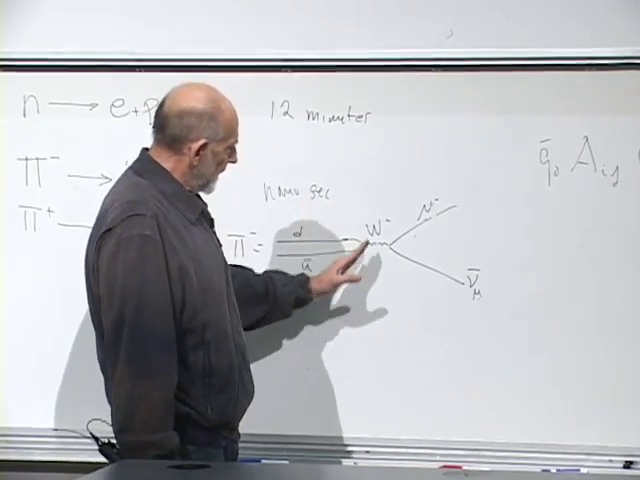
\includegraphics[width=0.72\textwidth]{lecture_05_figure_04.png}
\caption{Un pión \(d\bar u\) se aniquila y produce un \(W^-\) virtual, seguido de un leptón cargado y su antineutrino correspondiente.}
\lectureframe{01:19:38}
\end{figure}

\begin{classroomqa}\audiencequestion{¿Sigue siendo esto realmente un diagrama de Feynman aunque la dirección del tiempo se haya dibujado en horizontal y no en vertical?
\lecturetimestamp{01:20:21}}\lecturerresponse{Sí. La orientación del tiempo en la página es una convención. Una vez declarada una dirección como temporal e interpretadas todas las flechas de manera coherente, el dibujo contiene la misma información sobre la interacción.}\end{classroomqa}

\begin{classroomqa}\audiencequestion{¿Podría leerse el diagrama como una reacción química reversible, en lugar de como una desintegración irreversible en un solo sentido?
\lecturetimestamp{01:21:35}}\lecturerresponse{El proceso inverso está permitido. Un pión producido en el espacio vacío se desintegra porque las partículas salientes se separan y normalmente no vuelven a combinarse. Pero si se hacen colisionar un muón y un antineutrino con la energía y el momento adecuados, existe una amplitud no nula para formar el pión mediante la interacción inversa.}\end{classroomqa}

\subsection{Energía y estado intermedio virtual}

Para un pión en reposo,
\begin{equation}
m_\pi\simeq140\ {\rm MeV},
\qquad
m_\mu\simeq106\ {\rm MeV},
\qquad
m_\nu\approx0
\end{equation}
con la precisión pertinente aquí. La energía restante se convierte en energía cinética de las partículas salientes. La conservación del momento exige
\begin{equation}
\boldsymbol p_\mu+\boldsymbol p_{\bar\nu}=0,
\end{equation}
por lo que las dos partículas salen en direcciones opuestas en el sistema de referencia en reposo del pión.

\begin{classroomqa}\audiencequestion{¿Cómo puede conservarse la energía si el \(W\) intermedio tiene una masa muy superior a la del pión?
\lecturetimestamp{01:25:08}}\lecturerresponse{Solo las partículas iniciales y finales deben estar en su capa de masa. El cuadrimomento se conserva en cada vértice, pero una línea virtual interna no tiene por qué satisfacer \(E^2=\boldsymbol p^2+m_W^2\). Cuanto mayor es su desviación respecto de la capa de masa, más suprime el proceso su propagador.\editorialnote{La clase recurre al lenguaje tradicional de la incertidumbre energía--tiempo y dice que el estado intermedio puede violar brevemente la conservación de la energía. La formulación moderna y precisa es la de la respuesta: se conserva la energía y el momento, mientras que una línea interna virtual no tiene por qué satisfacer la condición de capa de masa de una partícula real.}}
\end{classroomqa}

\subsection{Desintegración del muón}

Un muón puede transformarse primero en su propio neutrino al emitir un \(W^-\) virtual:
\begin{equation}
\mu^-\longrightarrow\nu_\mu+W^{-*}.
\end{equation}
El bosón virtual produce luego un electrón y un antineutrino electrónico:
\begin{equation}
\mu^-\longrightarrow
\nu_\mu+e^-+\bar\nu_e.
\label{eq:l5-muon-decay}
\end{equation}
Este es un proceso puramente leptónico. El muón tiene una masa unas doscientas veces mayor que la del electrón, así que las masas en reposo finales dejan energía cinética suficiente.

\begin{figure}[htbp]
\centering
\includegraphics[width=0.72\textwidth]{lecture_05_figure_06.png}
\caption{Desintegración del muón a través de un bosón débil cargado virtual.}
\lectureframe{01:29:24}
\end{figure}

\begin{classroomqa}
\audiencequestion{¿La partícula neutra emitida junto con el electrón es un
antineutrino?
\lecturetimestamp{01:29:06}}
\lecturerresponse{Sí. El estado final completo contiene un neutrino muónico, un
antineutrino electrónico y el electrón. Mantener las etiquetas de sabor evita
confundir las dos partículas neutras.}
\end{classroomqa}

El electrón no puede invertir este decaimiento en el espacio vacío porque es más ligero que el muón. El tau es más pesado y puede decaer por canales débiles análogos. La estabilidad en este caso se debe en parte a una coincidencia del orden de las masas, no a una diferencia en el vértice subyacente.

\begin{classroomqa}
\audiencequestion{¿Un acelerador lineal aumenta, en la práctica, la masa del
electrón para que las reacciones que de otro modo estarían prohibidas puedan
producirse en sentido contrario?
\lecturetimestamp{01:30:23}}
\lecturerresponse{No cambia la masa invariante en reposo del electrón, pero
le proporciona energía cinética. Una energía suficiente en el centro de masas
puede crear partículas finales más pesadas; por tanto, la idea física propuesta
es correcta si se sustituye la masa por la energía de colisión disponible.}
\end{classroomqa}

\subsection{Decaimiento beta del neutrón a nivel de quarks}

Las composiciones de quarks de valencia del neutrón y el protón son
\begin{equation}
n=udd,
\qquad
p=uud.
\end{equation}
Un quark down del neutrón experimenta la transición de corriente cargada
\begin{equation}
d\longrightarrow u+W^{-*},
\end{equation}
que convierte \(udd\) en \(uud\). Luego, el bosón virtual decae:
\begin{equation}
W^{-*}\longrightarrow e^-+\bar\nu_e.
\end{equation}
La combinación de ambos vértices reproduce
\begin{equation}
n\longrightarrow p+e^-+\bar\nu_e.
\end{equation}

La transición inversa del quark \(u\to d+W^+\) daría lugar a un barión formado por tres quarks down, pero ese estado accesible tiene demasiada masa para que lo produzca un neutrón libre. La vía real de down a up es la que está permitida energéticamente.

\begin{classroomqa}
\audiencequestion{¿Podría decaer un neutrón en un protón, un muón y el
antineutrino correspondiente?
\lecturetimestamp{01:32:38}}
\lecturerresponse{No, si el neutrón libre está en reposo: la diferencia de masas entre el neutrón--y el protón es mucho menor que la masa del muón. Con suficiente energía adicional de colisión o de excitación, el mismo vértice débil puede participar en un canal que produzca un muón. La prohibición es cinemática; no se debe a la ausencia de una interacción.}
\end{classroomqa}

\section{La supresión aún sin explicar}

Los vértices débiles cargados explican qué procesos pueden ocurrir, pero todavía no por qué son tan lentos. Una respuesta tentadora sería que el acoplamiento débil es extraordinariamente pequeño. Esa respuesta es incorrecta: el acoplamiento gauge débil adimensional es de un orden de magnitud similar al electromagnético. La supresión debe tener otro origen.

El ingrediente que falta ya se aprecia en el propagador virtual: el \(W\) tiene una masa muy grande. A energías muy inferiores a \(m_W\), las amplitudes de corriente cargada se suprimen aproximadamente mediante potencias de \(1/m_W^2\). Esta conexión se desarrollará después de explicar cómo el mecanismo de Higgs y la ruptura de la simetría electrodébil dan masa a los bosones gauge.
\editorialnote{La clase deja planteada esta cuestión para la próxima sesión. La explicación basada en el bosón pesado \(W\) se incluye aquí como anticipo, no como afirmación de que su derivación haya tenido lugar en esta clase.}

\begin{classroomqa}
\audiencequestion{Cuando decimos que la teoría tiene esta simetría, ¿queremos
decir que su lagrangiano es invariante bajo las operaciones correspondientes?
\lecturetimestamp{01:34:14}}
\lecturerresponse{Exactamente. Decir que la teoría tiene la simetría es una
forma abreviada de afirmar que el lagrangiano, o equivalentemente la acción, es
invariante bajo esas transformaciones. La escritura del lagrangiano completo se
pospone; no se sustituye por una definición distinta.}
\end{classroomqa}

La exposición llega así a su conclusión: la teoría de Maxwell proporciona el prototipo; la cromodinámica cuántica muestra cómo los bosones gauge no abelianos transportan e intercambian carga; las constantes de acoplamiento explican el contraste entre las escalas de tiempo atómicas y hadrónicas; y \(SU(2)\) organiza los quarks y los leptones en dobletes conectados por \(W^\pm\). Queda por entender por qué, en la práctica, estos procesos mediados por bosones gauge son débiles, aunque el acoplamiento subyacente no sea excepcionalmente pequeño.

\chapter{Intercambio débil masivo, partículas virtuales y simetría rota}

El grupo del modelo estándar resulta mucho menos misterioso si lo interpretamos como un conjunto de movimientos permitidos en la tabla de fermiones. Las transformaciones de color se desplazan verticalmente entre rojo, verde y azul. Las transformaciones débiles cargadas se desplazan horizontalmente dentro de los dobletes de quarks y leptones. Las transformaciones de fase electromagnéticas aportan una tercera operación. Los bosones de gauge correspondientes no son adornos añadidos después de descubrir las simetrías: la emisión de un bosón de gauge realiza físicamente el mismo cambio de estado que describe un generador de la simetría.

Esta observación plantea la pregunta central de esta lección. Un vértice débil tiene un acoplamiento de magnitud comparable al de un vértice electromagnético, y, sin embargo, la desintegración beta es muchísimo más lenta que un proceso fuerte o electromagnético típico. El ingrediente que falta es la propagación. A bajo momento, el intercambio de un \(W\) cuesta un factor del orden de \(1/m_W^2\) en la amplitud. Primero desarrollaremos esta afirmación en el espacio de distancias y luego en el espacio de momentos; seguiremos sus consecuencias en una larga discusión sobre partículas reales y virtuales y, por último, abordaremos el primer modelo cualitativo de la ruptura espontánea de la simetría.

\section{Leer la simetría de gauge en la tabla de fermiones}

\subsection{El color actúa verticalmente}

Dispongamos los seis sabores de quarks en tres familias débiles:
\begin{equation}
  (u,d),\qquad(c,s),\qquad(t,b),
\end{equation}
y asignemos a cada quark una etiqueta de color rojo, verde o azul. La tabla de quarks resultante tiene tres filas de colores y seis columnas de sabores. El color \(SU(3)\) mezcla las tres entradas de cualquier columna de sabor. Por ejemplo, un generador puede transformar un quark up rojo en un quark up verde. En el lenguaje de las partículas, la misma operación va acompañada de la emisión de un gluón que lleva el color y el anticolor compensatorios.

La misma transformación de color debe actuar sobre todos los sabores. El gluón que transforma un quark up rojo en uno verde es la misma especie de gluón que transforma un quark top rojo en uno verde. Una verdadera operación de simetría no se aplica a la primera generación ignorando las demás. Así pues, el movimiento del color es vertical y universal:
\begin{equation}
  q_r\longleftrightarrow q_g\longleftrightarrow q_b,
  \qquad q\in\{u,d,c,s,t,b\}.
\end{equation}
Cambia el color, pero no el sabor.

Esta es la relación característica entre un grupo de gauge y sus bosones de gauge. Los generadores infinitesimales describen transformaciones entre estados, y la emisión o absorción de los bosones correspondientes realiza esas transformaciones como procesos físicos.

\subsection{Las transformaciones débiles actúan horizontalmente}

La interacción débil cargada se desplaza en la otra dirección. Un quark de tipo up puede emitir un bosón débil cargado y convertirse en su compañero de tipo down sin cambiar de color:
\begin{equation}
  u_b\longrightarrow d_b+W^+.
\end{equation}
Exactamente el mismo \(W^+\) aparece en
\begin{equation}
  c_g\longrightarrow s_g+W^+,
  \qquad
  t_r\longrightarrow b_r+W^+.
\end{equation}
Las etiquetas \(r,g,b\) no intervienen. Los gluones no se desplazan horizontalmente por la tabla, y los bosones cargados \(W\) no se desplazan verticalmente a través de los colores.

Añadamos la simetría de fase electromagnética \(U(1)\), bajo la cual todo campo cargado adquiere una fase. La estructura de grupo en una primera aproximación es entonces
\begin{equation}
  SU(3)\times SU(2)\times U(1).
\end{equation}
Los signos de producto indican que se trata de factores independientes: uno actúa sobre el color, otro sobre los dobletes débiles y el tercero mediante una fase. Esta imagen aproximada resulta útil, pero aún no describe por completo la teoría electrodébil.\editorialnote{El grupo de gauge exacto del modelo estándar se escribe convencionalmente como \(SU(3)_c\times SU(2)_L\times U(1)_Y\). El grupo débil \(SU(2)_L\) actúa solo sobre dobletes levógiros, y el grupo electromagnético final \(U(1)_{\rm em}\) surge de \(SU(2)_L\times U(1)_Y\) tras la ruptura de la simetría. La lección advierte explícitamente que la identificación inicial de los dos últimos factores todavía no es plenamente coherente; las lecciones posteriores aportan la estructura quiral y electrodébil que falta.}

\subsection{El mismo patrón incluye a los leptones}

Debajo de las tres filas de colores, coloquemos una fila de leptones sin color:
\begin{equation}
\begin{array}{c|cc|cc|cc}
 &u&d&c&s&t&b\\ \hline
Q&+\frac23&-\frac13&+\frac23&-\frac13&+\frac23&-\frac13\\
\text{lepton partner}
 &\nu_e&e^-&\nu_\mu&\mu^-&\nu_\tau&\tau^-\\
Q&0&-1&0&-1&0&-1
\end{array}
\end{equation}
En cada par adyacente, las cargas eléctricas difieren en una unidad. Por eso el mismo bosón débil cargado puede conectar \(u\) con \(d\), \(c\) con \(s\), \(t\) con \(b\), y un leptón cargado con su neutrino. Al vértice \(W\) le importan los números cuánticos pertinentes y la diferencia de carga, no si el fermión es un quark o un leptón.

\begin{figure}[htbp]
\centering
\includegraphics[width=0.88\textwidth]{lecture_06_figure_07.png}
\caption{La tabla completa de fermiones: tres filas de quarks con color, encima de la fila de leptones sin color; se muestran las cargas de los quarks y los tres dobletes de leptones.}
\lectureframe{00:18:55}
\end{figure}

El muón tiene la misma carga y los mismos números cuánticos intrínsecos conocidos que el electrón, pero es unas doscientas veces más pesado. El tau es aún más pesado. Las masas de los neutrinos son muy pequeñas y, en la discusión de la lección, no se conocían en detalle. Hasta aquí no ha surgido ningún principio que explique el patrón observado de masas de las familias.

\begin{classroomqa}
\audiencequestion{¿Por qué se llama leptones, bariones y mesones a estas partículas?
\lecturetimestamp{00:19:02}}
\lecturerresponse{Las raíces griegas históricas significaban, aproximadamente, ligero, pesado e intermedio. Esta nomenclatura basada en la masa acabó resultando engañosa. Al muón se lo llamó en otro tiempo mesón mu porque su masa estaba entre las del electrón y el protón, pero sus interacciones muestran que es un leptón, mucho más parecido a un electrón que a un pión. Hoy, un mesón es un hadrón formado por un quark--antiquark y es un bosón; el muón no es un mesón.}
\end{classroomqa}

\section{El enigma de la debilidad}

\subsection{Un proceso concreto de corriente cargada}

Tomemos la desintegración beta del neutrón como diagrama de trabajo. Las composiciones de quarks de valencia son
\begin{equation}
  n=udd,\qquad p=uud.
\end{equation}
Un quark down experimenta la transición
\begin{equation}
  d\longrightarrow u+W^-,
\end{equation}
y el bosón cargado produce
\begin{equation}
  W^-\longrightarrow e^-+\bar\nu_e.
\end{equation}
En conjunto,
\begin{equation}
  n\longrightarrow p+e^-+\bar\nu_e.
\end{equation}
Los otros dos quarks de valencia siguen como espectadores. En el primer vértice, el neutrón se convierte en un protón; en el segundo, la misma interacción débil que conecta un doblete de leptones convierte el \(W^-\) en el electrón y el antineutrino electrónico observados.

\subsection{Tres acoplamientos, tres impresiones muy distintas}

En la electrodinámica cuántica, la carga del electrón \(e\) es la amplitud del vértice. Al elevarla al cuadrado se obtiene la probabilidad característica de emisión, con los factores convencionales agrupados en
\begin{equation}
  \alpha=\frac{e^2}{4\pi}\simeq\frac1{137}
\end{equation}
en unidades naturales. La interacción fuerte tiene un acoplamiento \(g_s\) y, a una escala hadrónica típica, su análogo \(\alpha_s\) puede ser del orden de \(0.2\). Esto es mucho mayor que \(1/137\), así que la emisión de gluones es frecuente cuando se golpea un quark.

Sea \(g_w\) el acoplamiento débil cargado. Su cuadrado no es extraordinariamente pequeño; en el orden de magnitud usado aquí es comparable al acoplamiento electromagnético. Aun así, un neutrón libre espera unos quince minutos antes de desintegrarse, mientras que una desintegración fuerte puede ocurrir en un tiempo de cruce hadrónico. La estimación histórica de la lección usa la cifra aproximada, más antigua, de doce minutos, pero cualquiera de las dos cifras plantea el mismo enigma inevitable.\editorialnote{La vida media moderna del neutrón libre es de aproximadamente \(8.8\times10^2\,{\rm s}\), y persiste una discrepancia experimental entre los principales métodos de medición. Se conserva la estimación aproximada de la lección como escala pedagógica, no como valor de precisión.}
\begin{quote}
Si \(g_w\) no es extraordinariamente pequeño, ¿qué hace débiles a los procesos débiles?
\end{quote}

La respuesta no puede estar solo en los vértices. Todo diagrama de Feynman contiene también propagadores, los factores que describen la evolución intermedia de un vértice a otro.

\section{Un propagador masivo en el espacio de distancias}

\subsection{Los vértices no son todo el diagrama}

El diagrama de desintegración beta contiene dos vértices débiles, que aportan dos potencias de \(g_w\), y una línea de \(W\) que los une. Denotemos por \(\Delta(x-y)\) el propagador en el espacio de posiciones, donde \(x\) es el evento de emisión y \(y\) el evento de absorción o conversión. Es el núcleo de amplitud asociado al transporte de la perturbación del campo entre esos eventos.

El propagador relativista exacto contiene más estructura de la que necesitamos. Su característica cualitativa importante es su dependencia de la masa. A distancias cortas de tipo espacial presenta una singularidad de ley de potencias, esquemáticamente
\begin{equation}
  \Delta(d)\sim\frac1{d^2}.
\end{equation}
Un campo sin masa conserva una cola de ley de potencias. En cambio, un campo masivo queda exponencialmente suprimido cuando la separación es grande comparada con su escala de Compton. Por tanto, la curva del gráfico cae bruscamente.

\subsection{Las unidades naturales sitúan el cambio de pendiente}

Fijemos
\begin{equation}
  c=\hbar=1.
\end{equation}
Entonces,
\begin{equation}
  [m]=[E]=[p]=L^{-1}.
\end{equation}
Las relaciones conocidas explican cada igualdad: \(E=mc^2\) identifica masa y energía, mientras que \(p\,x\) tiene las dimensiones de \(\hbar\), de modo que el momento y la distancia tienen unidades inversas. Por tanto, la única longitud que puede formarse a partir de la masa \(m\) es
\begin{equation}
  d_m\sim\frac1m.
\end{equation}
Al restablecer las constantes se obtiene
\begin{equation}
  d_m\sim\frac{\hbar}{mc},
\end{equation}
la longitud de onda de Compton. Cuanto más pesada es la partícula intercambiada, menor es su alcance efectivo.

\begin{figure}[htbp]
\centering
\includegraphics[width=0.78\textwidth]{lecture_06_figure_02.png}
\caption{Dimensiones en unidades naturales y decaimiento cualitativo del propagador. La curva negra continúa con una cola de ley de potencias; la curva roja, correspondiente a una partícula masiva, cae cerca de la escala inversa de la masa.}
\lectureframe{00:27:19}
\end{figure}

\begin{figure}[htbp]
\centering
\begin{tikzpicture}[x=1.0cm,y=0.9cm]
  \draw[->] (0,0) -- (7,0) node[right] {$d$};
  \draw[->] (0,0) -- (0,5) node[above] {$|\Delta(d)|$};
  \draw[thick]
    plot[smooth] coordinates {(0.45,4.5) (0.9,3.3) (1.6,2.5)
      (2.5,1.9) (3.7,1.45) (5.1,1.12) (6.4,0.9)};
  \draw[thick,red]
    plot[smooth] coordinates {(0.45,4.5) (0.9,3.3) (1.6,2.5)
      (2.5,1.9) (3.2,1.55) (3.7,0.95) (4.2,0.36) (4.8,0.1)};
  \draw[dashed] (3.4,0) -- (3.4,1.4);
  \node at (5.7,1.4) {$m=0$};
  \node[red] at (4.75,0.72) {$m>0$};
  \node[below] at (3.4,0) {$d\sim m^{-1}$};
\end{tikzpicture}
\caption{Esquema claro del argumento de la pizarra. No es una fórmula exacta para un propagador en cuatro dimensiones; aísla el alcance controlado por la masa.}
\end{figure}

\begin{classroomqa}
\audiencequestion{¿Qué se representa en el eje vertical?
\lecturetimestamp{00:28:30}}
\lecturerresponse{La magnitud del propagador, denotada por \(\Delta\). Su cuadrado contribuye a una probabilidad una vez que se incluyen la amplitud completa, los estados externos y los factores de espacio de fases. El gráfico pretende mostrar que la amplitud de intercambio masivo a larga distancia se anula rápidamente.\editorialnote{Un propagador por sí solo no es una amplitud de probabilidad directamente medible de una partícula que sigue una trayectoria clásica. El lenguaje de la lección sirve para estimar el alcance: el propagador es uno de los factores de la amplitud completa de dispersión o desintegración.}}
\end{classroomqa}

\section{Transformada de Fourier y límite de Fermi}

\subsection{Los experimentos especifican momentos}

Un experimento suele medir los momentos externos, en lugar de los dos puntos del espacio-tiempo donde empieza y termina una línea interna. En la desintegración beta, el momento que lleva el \(W\) se infiere de la diferencia entre los momentos del neutrón y del protón, y es igual al momento total del electrón y el antineutrino. Los propagadores en el espacio de posiciones y en el espacio de momentos están relacionados mediante una transformada de Fourier.
\begin{equation}
  k=p_n-p_p=p_e+p_{\bar\nu_e}.
\end{equation}

Con la convención de denominador positivo usada en la pizarra,
\begin{equation}
  \widetilde{\Delta}_W(k)=\frac1{k^2+m_W^2},
  \qquad
  \widetilde{\Delta}_\gamma(k)=\frac1{k^2}.
\end{equation}
El propagador del fotón sin masa se hace grande para una transferencia de momento pequeña. El propagador masivo del \(W\) nunca supera una escala del orden de \(1/m_W^2\). En la desintegración beta,
\begin{equation}
  |k^2|\ll m_W^2,
\end{equation}
de modo que los detalles de \(k^2\) son despreciables y
\begin{equation}
  \widetilde{\Delta}_W(k)\simeq\frac1{m_W^2}.
\end{equation}

\begin{classroomqa}
\audiencequestion{¿No debería el \(k^2\) relativista contener un signo menos entre la energía y el momento espacial?
\lecturetimestamp{00:35:11}}
\lecturerresponse{Sí. Con una métrica de Minkowski de signatura mayoritaria negativa,
\(k^2=(k^0)^2-\boldsymbol{k}^2\), y el denominador escalar se escribe convencionalmente como \(k^2-m_W^2+i\epsilon\). En la pizarra se usa la magnitud positiva equivalente, de tipo espacial o euclídea. En la desintegración beta de baja energía, el cuadrimomento transferido es minúsculo comparado con \(m_W\), así que ambas notaciones dan la misma supresión \(1/m_W^2\), salvo por un signo irrelevante en la amplitud.}
\end{classroomqa}

\subsection{La amplitud de baja energía}

Dos vértices débiles y un propagador dan
\begin{align}
  \mathcal A_{\rm weak}
  &\sim g_w\,\widetilde{\Delta}_W(k)\,g_w\\
  &\sim\frac{g_w^2}{k^2+m_W^2}
  \simeq\frac{g_w^2}{m_W^2}.
\end{align}
Al elevar la amplitud al cuadrado se obtiene la supresión característica
\begin{equation}
  |\mathcal A_{\rm weak}|^2
  \sim\frac{g_w^4}{m_W^4},
\end{equation}
antes de incluir los factores cinemáticos y de espacio de fases propios de la desintegración concreta. La interacción débil es débil a energías nucleares no porque su acoplamiento de gauge elemental sea absurdamente pequeño, sino porque su mediador es pesado.

\begin{figure}[htbp]
\centering
\includegraphics[width=0.86\textwidth]{lecture_06_figure_03.png}
\caption{El proceso débil entre el neutrón--y el protón y la transferencia de momento que lleva la línea interna, tal como se discutieron al fijar el signo del propagador.}
\lectureframe{00:35:40}
\end{figure}

\begin{figure}[htbp]
\centering
\includegraphics[width=0.84\textwidth]{lecture_06_figure_04.png}
\caption{La topología de la desintegración beta junto a la estimación de baja energía enmarcada
\(g_w^2/m_W^2\).}
\lectureframe{00:37:25}
\end{figure}

Numéricamente, \(m_W\) es aproximadamente cien veces la masa del protón, con la precisión de esta lección. Un factor de \(m_W^{-2}\) en la amplitud se convierte en \(m_W^{-4}\) en una tasa, así que incluso un acoplamiento de magnitud ordinaria en una teoría de gauge produce una vida media muy larga.

\begin{classroomqa}
\audiencequestion{¿Hablamos de una supresión de una entre un millón o de una entre mil millones, y cómo se conoció originalmente la masa del \(W\)?
\lecturetimestamp{00:38:11}}
\lecturerresponse{El cálculo aproximado de la lección apunta a una pequeñez del orden de mil millones para la probabilidad débil de baja energía en comparación con un proceso hadrónico sin supresión. Históricamente, los experimentos de baja energía no midieron por separado \(g_w\) y \(m_W\). Midieron la pequeña combinación \(g_w^2/m_W^2\), llamada constante de Fermi. Una vez que se vinculó el acoplamiento a la teoría electrodébil, esa combinación predijo un mediador muy pesado; más tarde, los aceleradores produjeron directamente el \(W\) y midieron su masa.}
\end{classroomqa}

A momentos muy inferiores a \(m_W\), todos los experimentos observan prácticamente la misma constante:
\begin{equation}
  G_F\sim\frac{g_w^2}{m_W^2}.
\end{equation}
Por eso Fermi pudo describir la desintegración beta en la década de 1930 como una interacción puntual de cuatro fermiones, mucho antes de que se observara el mediador. Al aumentar las energías de colisión, los experimentos se hicieron sensibles a la dependencia del momento oculta en el propagador y confirmaron que la constante efectiva era la huella, a baja energía, del intercambio de una partícula masiva.\editorialnote{Con la normalización electrodébil estándar al nivel de árbol,
\[
  \frac{G_F}{\sqrt2}=\frac{g^2}{8m_W^2}.
\]
La lección omite deliberadamente los factores numéricos y de espinores, y conserva solo el escalamiento \(G_F\sim g_w^2/m_W^2\). Los bosones \(W\) y \(Z\) se descubrieron directamente en el CERN en 1983; la referencia pasajera de la lección a mediados o finales de la década de 1970 es demasiado temprana para su observación directa.}

Históricamente, la idea de que las interacciones débiles podían estar mediadas por una partícula pesada surgió a mediados del siglo XX; la lección menciona a Julian Schwinger entre los teóricos que exploraron esa posibilidad y señala que la letra \(W\) probablemente significaba débil. Los datos de baja energía ya indicaban que ese mediador tendría que ser extremadamente pesado a escala nuclear, mucho antes de que los aceleradores alcanzaran energía suficiente para producirlo como partícula real.

\subsection{Tres factores independientes que controlan una tasa}

Una pregunta en clase sobre la energía de enlace nuclear permite distinguir tres factores de una transición, distintos desde el punto de vista lógico:
\begin{enumerate}
  \item constantes de acoplamiento de los vértices;
  \item propagadores, incluidas las masas y la dependencia del momento;
  \item energía disponible entre el estado inicial y el final, y espacio de fases.
\end{enumerate}
La energía de enlace puede cerrar un canal de desintegración porque el estado final tendría más energía que el inicial. Se trata de una prohibición cinemática, no de una reducción adicional de \(g_w\) ni de un cambio en \(m_W\). Si un canal sigue abierto pero queda poca energía disponible, su espacio de fases también puede estar fuertemente suprimido.

\begin{classroomqa}
\audiencequestion{¿El campo o la energía de enlace de un protón cercano suprimen la desintegración beta mediante el mismo mecanismo del propagador?
\lecturetimestamp{00:41:13}}
\lecturerresponse{No en el ejemplo que estamos tratando. La energía de enlace importa porque cambia las energías de los estados nucleares inicial y final. Un proceso no puede ocurrir si el estado final es inaccesible desde el punto de vista energético. Los acoplamientos, los propagadores y la energía disponible son tres ingredientes distintos.}
\end{classroomqa}

\begin{classroomqa}
\audiencequestion{¿Las constantes de acoplamiento son realmente constantes?
\lecturetimestamp{00:42:55}}
\lecturerresponse{Solo a una escala fija. Las correcciones cuánticas hacen que los acoplamientos efectivos dependan del momento o de la distancia. En el argumento actual, cada acoplamiento se considera a la escala pertinente para el proceso; más adelante se desarrollará la dependencia con la escala.}
\end{classroomqa}

\section{Intercambio virtual sin abandonar las leyes de conservación}

\subsection{Por qué puede aparecer la línea pesada}

La desintegración ordinaria del neutrón no contiene energía suficiente para producir un \(W\) libre y en su capa de masa. El \(W\) del diagrama es interno y está fuera de la capa de masa. La lección introduce este hecho mediante la estimación tradicional de energía--tiempo
\begin{equation}
  \Delta E\,\Delta t\lesssim\hbar:
\end{equation}
una configuración intermedia cuya energía clásica parece diferir en \(\Delta E\) solo puede contribuir durante un tiempo del orden de
\(\hbar/\Delta E\).

La analogía con el efecto túnel ilustra vívidamente la idea. Coloquemos una partícula alfa en un pozo de potencial nuclear. Su energía está por debajo de la cima de la barrera, así que clásicamente no puede escapar. Desde el punto de vista cuántico, la función de onda se extiende a través de la barrera, y la partícula puede aparecer en un punto del otro lado con la misma energía total que tenía inicialmente. Si intentamos describir el interior de la barrera como una trayectoria clásica ordinaria, la energía potencial parece demasiado grande y la energía cinética tendría que ser negativa. Esa imagen clásica fallida es análoga a intentar considerar el \(W\) interno como una partícula real.

\begin{figure}[htbp]
\centering
\includegraphics[width=0.78\textwidth]{lecture_06_figure_06.png}
\caption{La analogía con el efecto túnel: el punto inicial y el punto marcado en la pendiente opuesta tienen la misma energía total, mientras que la barrera intermedia está prohibida clásicamente.}
\lectureframe{00:46:00}
\end{figure}

\begin{figure}[htbp]
\centering
\begin{tikzpicture}[x=1.0cm,y=0.9cm]
  \draw[->] (0,0) -- (7,0) node[right] {$x$};
  \draw[->] (0,0) -- (0,4.8) node[above] {$V(x)$};
  \draw[thick]
    plot[smooth] coordinates {(0.3,1.4) (1.0,0.7) (1.7,0.55)
      (2.1,0.9) (3.2,3.9) (4.2,2.1) (5.0,0.75) (6.6,0.18)};
  \draw[dashed] (1.7,0.75) -- (5.0,0.75);
  \fill (1.7,0.75) circle (0.06);
  \fill (5.0,0.75) circle (0.06);
  \node at (3.35,0.35) {$\Delta E\,\Delta t\lesssim\hbar$};
\end{tikzpicture}
\caption{Una reconstrucción legible de la barrera y de los puntos con igual energía.}
\end{figure}

En la imagen de la desintegración beta, el neutrón puede fluctuar hacia un protón más un \(W^-\) interno, pero la línea pesada debe desaparecer rápidamente. Puede ser reabsorbido y restaurar el neutrón, o terminar en el segundo vértice y producir el electrón y el antineutrino, mucho más ligeros. Las energías inicial y final totales coinciden.\editorialnote{La energía y el momento se conservan en cada vértice de Feynman. Las partículas virtuales no toman literalmente energía prestada para devolverla después. La afirmación precisa es que se integra sobre los cuadrimomentos de una línea interna, los cuales no tienen por qué satisfacer la relación de capa de masa de una partícula real \(k^2=m_W^2\). Se conserva el lenguaje del principio de incertidumbre y del efecto túnel porque es la vía explicativa de la lección, pero la formulación moderna en teoría cuántica de campos es la condición fuera de la capa de masa.}

\subsection{Bosones W reales}

Un acelerador con energía suficiente puede producir un \(W\) real. Este tiene entonces su propia vida media propia, independiente del supuesto tiempo de incertidumbre de la línea virtual. Un \(W\) real en movimiento vive más tiempo en el laboratorio debido a la dilatación temporal relativista ordinaria. En una desintegración leptónica de dos cuerpos de un \(W\) en reposo,
\begin{equation}
  W^-\longrightarrow e^-+\bar\nu_e,
\end{equation}
el electrón y el antineutrino llevan energías cinéticas grandes y casi opuestas, cada una del orden de \(m_W/2\). La energía en reposo no ha desaparecido: se ha convertido en energía del estado final. También están disponibles los canales de muones y taus, así como los canales de quarks.

\begin{classroomqa}
\audiencequestion{¿Cuánto vive un \(W\) real y puede calcularse su vida media a partir del mismo acoplamiento?
\lecturetimestamp{00:49:49}}
\lecturerresponse{Sí. Se calcula la amplitud de cada desintegración permitida, se eleva al cuadrado, se integra sobre el espacio de fases del estado final y se suman las anchuras parciales. La inversa de la anchura total da la vida media. La estimación numérica oral de la transcripción es confusa, pero la idea cualitativa es que la vida media propia es extremadamente corta y un \(W\) en movimiento sufre la dilatación temporal habitual.\editorialnote{Usando la anchura medida \(\Gamma_W\simeq2.1\,{\rm GeV}\) se obtiene
\(\tau_W=\hbar/\Gamma_W\simeq3.2\times10^{-25}\,{\rm s}\). Este valor moderno resuelve el intercambio numérico transcrito de forma corrupta sin atribuírselo a la lección.}}
\end{classroomqa}

\begin{classroomqa}
\audiencequestion{¿Cómo se convierte una amplitud al cuadrado en una tasa y, por tanto, en una vida media?
\lecturetimestamp{00:50:52}}
\lecturerresponse{El elemento de matriz al cuadrado se combina con la densidad de estados finales disponibles, las funciones delta de conservación y los factores de normalización para obtener una probabilidad por unidad de tiempo: la anchura de desintegración \(\Gamma\). La probabilidad de supervivencia es \(e^{-\Gamma t}\) en unidades con \(\hbar=1\), así que \(\tau=1/\Gamma\), o bien \(\tau=\hbar/\Gamma\) al restablecer las unidades. Por tanto, una anchura débil pequeña implica una vida media débil larga.}
\end{classroomqa}

\begin{classroomqa}
\audiencequestion{¿Se puede asignar una velocidad a una partícula que atraviesa la barrera por efecto túnel?
\lecturetimestamp{00:52:42}}
\lecturerresponse{Se puede dividir una distancia inferida por un tiempo de tránsito inferido, pero esa cantidad no debe interpretarse como la velocidad de una partícula clásica ni de una señal. Intentar medir una trayectoria en el interior de la barrera modifica el estado y destruye el experimento de efecto túnel original.}
\end{classroomqa}

\section{¿Qué significa observar una partícula virtual?}

\subsection{Partículas externas y líneas internas}

Las partículas reales son los estados asintóticos entrantes y salientes que pueden prepararse o detectarse lejos de la región de interacción. Las partículas virtuales son líneas internas en una representación perturbativa de la amplitud. No son trayectorias ocultas adicionales en el detector.

\begin{classroomqa}
\audiencequestion{¿Hay una definición clara de la diferencia entre una partícula real y una virtual?
\lecturetimestamp{00:55:05}}
\lecturerresponse{Una partícula real es un estado externo en la capa de masa que entra en la región de interacción o sale de ella. Una partícula virtual es una línea interna fuera de la capa de masa en un diagrama de Feynman. Esta última forma parte de la expansión matemática; no es un objeto observado de manera independiente.}
\end{classroomqa}

Para resolver un proceso que dura solo \(\Delta t\), una sonda necesita frecuencias del orden de \(1/\Delta t\) y, por tanto, energía del orden de \(\hbar/\Delta t\). Un fotón con resolución suficiente para distinguir una partícula alfa bajo una barrera alta puede aportar la energía necesaria para elevarla hasta la región de la barrera. Del mismo modo, una sonda lo bastante energética para resolver el \(W\) interno, de vida corta, puede crear un \(W\) real. El intento de observación convierte el proceso original en otro experimento.

La lección lo expresa como una frustración cuántica recurrente: la intervención necesaria para comprobar la imagen de un estado intermedio prohibido aporta justamente la energía que vuelve real la configuración aparentemente prohibida.

\subsection{Fluctuaciones de un protón}

En teoría de perturbaciones, el estado de un protón contiene amplitudes para configuraciones como
\begin{equation}
  p\longleftrightarrow n+W^+,
\end{equation}
y, de manera análoga, un neutrón tiene
\begin{equation}
  n\longleftrightarrow p+W^-.
\end{equation}
Si no interviene otra interacción, el bosón interno se reabsorbe. En cambio, una sonda de alta energía puede dejar un \(W\) entre las partículas salientes. Se puede describir esto como expulsar una fluctuación o crear un \(W\). Cambia la forma de expresarlo; la afirmación medible sobre la amplitud del estado final es la misma.

\begin{classroomqa}
\audiencequestion{Cuando una sonda de alta energía produce un \(W\) saliente, ¿expulsa una partícula que ya estaba ahí o crea una nueva?
\lecturetimestamp{01:01:20}}
\lecturerresponse{Cualquiera de las dos imágenes puede organizar las matemáticas. Una descripción ordenada en el tiempo dice que el protón fluctuó a \(n+W^+\) y que la sonda extrajo el neutrón antes de que se reabsorbiera; otra dice que la colisión creó el \(W\) final. Lo que es invariante es la probabilidad calculada para el estado final observado, no un relato clásico único de lo que existía antes de la medición.}
\end{classroomqa}

Aumentar la energía de colisión no revela un inventario fijo de objetos que hubieran estado ocultos dentro del blanco. Abre muchos estados finales posibles: un \(W\), varios bosones, chorros de quarks, hadrones y otras partículas permitidas por los números cuánticos conservados. Incluso al golpear un campo elemental con suficiente energía pueden producirse protones y muchos otros objetos compuestos. Lo que sale no tiene por qué haber estado presente de antemano como constituyente. La lección lleva la idea hasta extremos cómicos: si la energía y los números cuánticos lo permiten, ni siquiera mesas, sillas o un átomo de hidrógeno quedan excluidos lógicamente como configuraciones finales extraordinariamente improbables. El chiste encierra una advertencia seria contra definir la elementalidad mediante un inventario ingenuo de los productos de una colisión.

\subsection{Fluctuaciones del vacío y temperatura}

Una fluctuación asociada a un protón no es lo mismo que un diagrama de vacío. La primera es un componente del estado de un protón interactuante; una fluctuación del vacío no tiene una línea externa de protón. En ambos casos, una sonda con energía suficiente puede producir partículas reales que correspondan a un estado final permitido. Por ejemplo, dos fotones energéticos pueden producir un par electrón--positrón cuando la energía del centro de masas supera el umbral.

\begin{classroomqa}
\audiencequestion{¿Dependen estas reacciones de la temperatura?
\lecturetimestamp{01:05:17}}
\lecturerresponse{La amplitud elemental no requiere un baño térmico.
La temperatura importa estadísticamente: un sistema a alta temperatura contiene muchas
partículas con gran energía cinética, por lo que se vuelven habituales las
colisiones que superan el umbral. Calentar un sistema que contiene una partícula
alfa ligada también puede aportar suficiente energía para escapar por encima de
la barrera, además del túnel cuántico. Unas pocas partículas energéticas aisladas
constituyen un haz; muchas partículas energéticas distribuidas térmicamente
constituyen un baño caliente.}
\end{classroomqa}

\begin{classroomqa}
\audiencequestion{¿El \(W\) emitido en una fluctuación del protón es una fluctuación
del vacío?
\lecturetimestamp{01:06:56}}
\lecturerresponse{No. El \(W\) interno en
\(p\leftrightarrow n+W^+\) es una fluctuación del estado del protón interactuante.
Un proceso virtual cerrado sin ningún protón externo es una fluctuación del vacío.
Ambos obedecen las mismas reglas de la teoría de campos, pero corresponden a amplitudes distintas.}
\end{classroomqa}

\begin{classroomqa}
\audiencequestion{¿Por qué se requiere el antineutrino en el vértice leptónico \(W\)?
\lecturetimestamp{01:08:51}}
\lecturerresponse{Aporta los números cuánticos leptónicos conservados y forma parte
del vértice básico de corriente cargada que conecta \(e\), \(\nu_e\) y \(W\).
La barra distingue el antineutrino electrónico saliente de un neutrino.}
\end{classroomqa}

\section{¿Hasta dónde puede llevarse la conversión de energía?}

A continuación, la clase lleva hasta un límite deliberadamente absurdo la regla según la cual la energía puede crear partículas. ¿Podría un grano de café convertirse en una tarta de chocolate?
No existe ningún proceso práctico de ese tipo, pero la teoría cuántica relativista
no impone que la materia final se parezca al objeto inicial. Exige energía suficiente,
las cargas conservadas correctas y una amplitud distinta de cero. Un kilogramo tiene una energía del orden de
\begin{equation}
  Mc^2\sim9\times10^{16}\ {\rm J},
\end{equation}
por lo que cualquier colisión microscópica que reuniera un objeto particular de escala kilogramo sería fantásticamente improbable.

La masa de Planck,
\begin{equation}
  m_{\rm P}=\sqrt{\frac{\hbar c}{G}}
  \simeq2.2\times10^{-5}\ {\rm g},
\end{equation}
no es una masa máxima posible. Es la escala a la que la gravedad se vuelve
intensa para un cuanto localizado en una región del tamaño de su longitud de onda de Compton. Un kilogramo contiene
aproximadamente \(5\times10^7\) masas de Planck.

\begin{classroomqa}
\audiencequestion{Si las colisiones superan la escala de Planck, ¿pueden surgir objetos de masa arbitrariamente grande, como sillas o planetas?
\lecturetimestamp{01:10:37}}
\lecturerresponse{A energías transplanckianas en el centro de masas concentradas en una
región pequeña, el resultado abrumadoramente más natural es el colapso gravitatorio:
un agujero negro. Un objeto macroscópico muy organizado sería una fluctuación
extraordinariamente rara. La clase invoca la inversión temporal: como una silla puede
caer en un agujero negro, la amplitud del proceso inverso no es exactamente cero.
Su probabilidad está suprimida por un factor entrópico enorme, así que no hay que
confundir posibilidad con probabilidad práctica.}
\end{classroomqa}

Esta digresión refuerza la advertencia anterior. La teoría cuántica de campos predice
amplitudes entre estados iniciales y finales especificados. Afirmar pintorescamente
que cada producto ya estaba literalmente contenido en el blanco antes del impacto
no forma parte de la predicción.

\section{Bosones, sus interacciones y su estadística}

\subsection{Los fotones pueden dispersarse}

Ser un bosón no significa carecer de interacciones. Ser bosón o fermión especifica
la estadística de intercambio; los vértices de interacción son hechos dinámicos
independientes. Los haces de luz clásicos suelen atravesarse porque la electrodinámica
cuántica no tiene un vértice de cuatro fotones al nivel de árbol y la dispersión
fotón--fotón a baja energía es extremadamente pequeña. Sin embargo, dos
fotones pueden interactuar mediante un lazo virtual de electrón--positrón:
\begin{equation}
  \gamma+\gamma
  \longrightarrow(e^-e^+)_{\rm virtual}
  \longrightarrow\gamma+\gamma.
\end{equation}
Si la energía en el centro de masas es suficientemente alta, en cambio, pueden crear
un par real,
\begin{equation}
  \gamma+\gamma\longrightarrow e^-+e^+.
\end{equation}
Los fotones ópticos tienen energías de unos pocos electronvoltios, mientras que el
umbral de creación de pares es del orden de \(2m_e c^2\approx1.02\,{\rm MeV}\). Por tanto, el proceso virtual
está muy suprimido a las energías ópticas habituales, razón por la cual los haces de luz que se cruzan parecen no afectarse entre sí.

\begin{classroomqa}
\audiencequestion{¿Los bosones \(W\) virtuales interactúan con otros bosones simplemente
porque son bosones?
\lecturetimestamp{01:12:47}}
\lecturerresponse{Pueden interactuar, pero no por el mero hecho de obedecer la estadística de Bose.
Los vértices de gauge determinan las interacciones dinámicas. La estadística,
en cambio, determina cómo se comportan las amplitudes de muchos cuerpos cuando se
intercambian partículas idénticas. Los fotones interactúan débilmente mediante
partículas virtuales cargadas, y la teoría electrodébil también contiene
autointeracciones no abelianas directas entre bosones \(W\).}
\end{classroomqa}

\subsection{La amplificación de Bose no es una fuerza}

La diferencia entre la estadística de fermiones y la de bosones se hace patente cuando
varias partículas idénticas ocupan estados cuánticos próximos. Los bosones favorecen la
ocupación múltiple; los fermiones excluyen la ocupación idéntica. En una colisión típica
de alta energía, las partículas salen hacia estados de momento bien separados, de modo
que este efecto estadístico puede ser menos evidente que en un láser o un condensado.

En principio, los bosones \(W\) presentan la misma amplificación de Bose. La clase
bromea con que podría imaginarse un sistema que emitiera radiación láser de bosones
\(W\). Su enorme masa y su vida media ultracorta hacen que un dispositivo así sea
fantásticamente impráctico, pero, efectivamente, su estadística es bosónica.

\begin{classroomqa}
\audiencequestion{¿De qué color es un protón o un neutrón?
\lecturetimestamp{01:18:41}}
\lecturerresponse{Un hadrón físico es un singlete de color, a menudo llamado
incoloro o blanco. Como regla mnemotécnica, se dice que un barión contiene un cuark
rojo, uno verde y uno azul. Más precisamente, su función de onda de color es la
superposición antisimétrica
\[
  |{\rm singlet}\rangle
  =\frac1{\sqrt6}\epsilon_{abc}|q^a q^b q^c\rangle,
\]
no una asignación clásica de un color permanente a cada cuark nombrado.}
\end{classroomqa}

\begin{classroomqa}
\audiencequestion{¿Se tratará la condensación de Bose en este curso?
\lecturetimestamp{01:19:25}}
\lecturerresponse{Sí, a través del fenómeno de Higgs. Un campo de Higgs distinto de cero en todo el vacío es análogo, en aspectos importantes, a un condensado bosónico. La analogía se desarrollará después de introducir la ruptura espontánea de la simetría.\editorialnote{El valor esperado en el vacío del campo de Higgs no es literalmente un gas ordinario de partículas de Higgs en su capa de masa que ocupen un mismo estado. La condensación es una analogía esclarecedora para un campo bosónico coherente y un vacío elegido, pero no constituye una identificación microscópica completa.}}
\end{classroomqa}

\section{El bosón débil neutro que falta}

Volvamos ahora a la tabla de grupos. Si la simetría débil horizontal es \(SU(2)\),
entonces tiene
\begin{equation}
  \dim SU(2)=3
\end{equation}
generadores y, por tanto, tres campos de gauge. Las combinaciones cargadas
\(W^+\) y \(W^-\) dan cuenta solo de dos. Se requiere un tercer campo neutro.
Está estrechamente relacionado con el bosón \(Z\) observado, pero no es simplemente el
fotón. Las combinaciones neutras precisas involucran tanto el tercer campo de
\(SU(2)_L\) como el campo \(U(1)_Y\). Esa mezcla, junto con la definición correcta
de la carga eléctrica, se pospone deliberadamente hasta la siguiente clase.

\section{Ruptura espontánea de simetría}

\subsection{Una elección simétrica puede dejar una indecisión inestable}

Imaginemos una mesa circular para una cena, con un cubierto a la izquierda y otro a
la derecha de cada puesto. Antes de que nadie se mueva, izquierda y derecha son
equivalentes. Cuando una persona se inclina hacia la derecha, todas las elecciones
de los puestos vecinos quedan determinadas, y toda la mesa acaba adoptando la
configuración hacia la derecha. Las reglas eran simétricas, pero la configuración
realizada seleccionó una de dos posibilidades. La historia es solo una analogía, pero
permite aislar la combinación que necesitamos: simetría, varios resultados equivalentes
y una inestabilidad que permite que una perturbación arbitrariamente pequeña
seleccione globalmente uno de ellos.

\subsection{La retícula de caras--cruces}

Para un modelo más sencillo, coloquemos una variable de dos estados \(s_i=\pm1\) en cada sitio de una
retícula. Llamemos \(+1\) cara y \(-1\) cruz. Supongamos que los sitios vecinos prefieren
alinearse:
\begin{equation}
  H=-J\sum_{\langle ij\rangle}s_i s_j,
  \qquad J>0.
\end{equation}
Los vecinos paralelos aportan menos energía que los antiparalelos.
Por tanto, hay dos estados fundamentales degenerados,
\begin{equation}
\begin{aligned}
  s_i&=+1\quad\text{for every }i,
  \\
  s_i&=-1\quad\text{for every }i.
\end{aligned}
\end{equation}
El hamiltoniano es invariante bajo la inversión global \(s_i\to-s_i\), pero ninguno de los estados fundamentales elegidos lo es.

Fijemos ahora en cara un espín de frontera muy distante. En un sistema ordinario de
corto alcance podríamos esperar que un grado de libertad muy lejano no tuviera
ninguna influencia aquí. Sin embargo, en la fase ordenada, esa condición de contorno
selecciona el vacío con todas las caras. Una vez seleccionado, una sola cruz en el
mar de caras cuesta energía porque no concuerda con sus vecinas. Las excitaciones
locales se definen respecto del estado fundamental elegido, aunque las ecuaciones
subyacentes conservan la simetría entre caras--cruces.

\subsection{Ruptura explícita y paredes de dominio}

La ruptura explícita añadiría un sesgo local,
\begin{equation}
  H_{\rm explicit}
  =-J\sum_{\langle ij\rangle}s_i s_j-h\sum_i s_i,
  \qquad h\ne0.
\end{equation}
De ese modo, caras y cruces no tienen la misma energía ni siquiera en un sitio aislado,
y solo hay un vacío preferido. En la ruptura espontánea, \(h=0\): las reglas locales
son simétricas y los dos vacíos siguen siendo degenerados, pero el sistema
ocupa uno de ellos.

Supongamos, en cambio, que la frontera del extremo izquierdo está toda en cara y la
del extremo derecho toda en cruz. La configuración de menor energía debe interpolar
entre los dos vacíos. La interfaz es una pared de dominio.

\begin{figure}[htbp]
\centering
\includegraphics[width=0.9\textwidth]{lecture_06_figure_08.png}
\caption{La retícula de caras--cruces dividida por una pared de dominio discontinua. Las condiciones de contorno opuestas obligan al sistema a contener una interfaz entre los dos estados ordenados degenerados.}
\lectureframe{01:30:35}
\end{figure}

\begin{classroomqa}
\audiencequestion{¿Qué distingue la ruptura espontánea de simetría de la ruptura ordinaria explícita de simetría?
\lecturetimestamp{01:28:36}}
\lecturerresponse{En la ruptura explícita, el hamiltoniano local ya asigna energías
Diferentes a caras y cruces, así que no hay un par de estados fundamentales
relacionados por simetría. En la ruptura espontánea, las ecuaciones conservan la
simetría, los vacíos son degenerados y las condiciones de contorno o una perturbación
arbitrariamente pequeña seleccionan uno de ellos. La posibilidad de una pared de
dominio que interpole entre vacíos distintos es un indicio de esta última situación.}
\end{classroomqa}

El modelo es deliberadamente primitivo, pero contiene la lógica esencial que se
trasladará al campo de Higgs: una teoría simétrica, una estructura de vacío inestable
o degenerada, un estado fundamental seleccionado y consecuencias físicas determinadas
por esa elección.

\section{Adónde nos lleva la clase}

La tabla de fermiones convierte el grupo del modelo estándar en un conjunto de
direcciones físicas. El color \(SU(3)\) avanza verticalmente entre rojo, verde y azul;
las transformaciones débiles cargadas avanzan horizontalmente a través de dobletes de
cuarks y leptones; una simetría de fase aporta el factor \(U(1)\) preliminar. La emisión
de bosones de gauge realiza estas transformaciones de grupo como interacciones.

La debilidad del decaimiento beta se atribuye entonces no a un \(g_w\) excepcionalmente
pequeño, sino al mediador pesado. En el espacio de distancias, la masa suprime el
propagador más allá de la escala de Compton \(\hbar/(m_Wc)\). En el espacio de momentos,
\begin{equation}
  \mathcal A_{\rm weak}
  \sim\frac{g_w^2}{k^2+m_W^2}
  \simeq\frac{g_w^2}{m_W^2}
\end{equation}
para momentos nucleares. Los antiguos experimentos de baja energía midieron esta combinación como
la constante de Fermi.

La extensa conversación en clase aclara qué significa y qué no significa esta fórmula.
Las líneas internas de \(W\) son virtuales y están fuera de la capa de masa; la energía--el momento
se conserva de todos modos. Una sonda suficientemente energética puede producir un \(W\) real, pero entonces
ha creado un proceso distinto con otro estado final. Los productos de una colisión no son una
lista literal de constituyentes preexistentes. La temperatura cambia la población
de proyectiles energéticos, los fotones pueden interactuar mediante partículas virtuales
cargadas y la estadística de Bose es distinta de una fuerza dinámica.

Por último, \(SU(2)\) requiere un campo de gauge neutro que falta, relacionado con el
\(Z\), y la retícula de caras--cruces proporciona el primer modelo de ruptura
espontánea de simetría. El siguiente paso es combinar esos dos hilos pendientes:
la mezcla electrodébil y el mecanismo de Higgs.

\chapter{Ruptura espontánea de la simetría, bosones de Goldstone e invariancia gauge}

Queremos entender cómo una partícula similar al fotón puede adquirir masa. Ese es el destino, pero no es un punto de partida sensato. Un término de masa directo para un campo gauge parece destruir precisamente la invariancia gauge que hace consistente la teoría. Antes de encontrar la salida, necesitamos manejar bien dos ideas:
\begin{enumerate}
  \item la ruptura espontánea de la simetría, especialmente cuando se trata de una simetría continua;
  \item la invariancia gauge, en la que la operación de simetría puede variar de un punto del espacio-tiempo a otro.
\end{enumerate}
Ninguna de estas ideas puede sustituirse por una consigna. Construiremos la primera a partir de un imán, la traduciremos al lenguaje de la teoría de campos escalares y descubriremos el modo de Goldstone sin masa. Luego tomaremos la misma \(U(1)\) simetría y la haremos local, lo que nos obligará a introducir un potencial vector y una derivada covariante. Solo al final pondremos ambos hilos uno junto al otro. Su unión propiamente dicha---el fenómeno de Higgs---será el tema de la próxima lección.

\section{Una ley simétrica con un estado fundamental asimétrico}

\subsection{El imán de dos estados}

Empecemos con una red de pequeños imanes. Cada espín puede apuntar hacia arriba o hacia abajo, y los espines vecinos reducen su energía al apuntar en la misma dirección. En una red cúbica tridimensional, cada espín tiene seis vecinos más próximos, pero el número exacto de vecinos no es importante. Lo que importa es la regla
\begin{equation}
  E_{\parallel}<E_{\rm antiparallel}.
\end{equation}
La regla microscópica no cambia si se invierten todos los espines:
\begin{equation}
  \uparrow\longleftrightarrow\downarrow.
\end{equation}
Sin embargo, las configuraciones de menor energía no son simétricas por separado. Son
\begin{equation}
  \{\uparrow\uparrow\uparrow\cdots\},
  \qquad
  \{\downarrow\downarrow\downarrow\cdots\}.
\end{equation}
Las ecuaciones permiten ambas, pero una muestra macroscópica fría debe elegir una.

Esta elección es extraordinariamente sensible. Fijemos un espín muy lejos para que apunte hacia arriba. Sus vecinos prefieren alinearse con él, los vecinos de estos prefieren alinearse con ellos, y la información se propaga por toda la muestra. Una perturbación arbitrariamente pequeña comparada con el sistema en su conjunto puede seleccionar la orientación de todo el estado fundamental. Esa es la inestabilidad a la que se refiere la ruptura \emph{espontánea} de la simetría.

\begin{classroomqa}
\audiencequestion{¿Puede una partícula neutra orientarse en un campo magnético?
\lecturetimestamp{00:05:14}}
\lecturerresponse{Sí. La neutralidad eléctrica no implica que no haya momento magnético. El neutrón es neutro, pero tiene un momento magnético debido a sus constituyentes cargados internos. Por tanto, un campo magnético puede distinguir entre sus orientaciones de espín.}
\end{classroomqa}

\begin{classroomqa}
\audiencequestion{Si el sistema cambia de orientación, ¿ocurre el cambio en todas partes a la vez? ¿Pueden coexistir varias ondas de reorientación?
\lecturetimestamp{00:05:41--00:06:38}}
\lecturerresponse{El cambio se propaga. Una región inclina a sus vecinas, como en una disposición tridimensional de fichas de dominó, y la perturbación viaja en forma de onda. Distintas regiones pueden empezar a elegir por separado, de modo que puede haber varios frentes y varios dominios antes de que prevalezca una orientación. Volveremos precisamente a estas ondas cuando la simetría sea continua.}
\end{classroomqa}

\subsection{La ruptura explícita corresponde a una teoría distinta}

Coloquemos ahora la muestra en un campo magnético externo que apunte hacia arriba. Un espín aislado ya tiene menor energía cuando apunta hacia arriba. La transformación \(\uparrow\leftrightarrow\downarrow\) deja de mantener constante la energía: la preferencia se ha incorporado a la propia ley. Esto es una ruptura \emph{explícita} de la simetría.

La diferencia puede comprobarse sin saber cómo se preparó la muestra. Tomemos una muestra muy grande, mantengamos su borde izquierdo hacia arriba y su borde derecho hacia abajo. Si un campo magnético en el volumen favorece explícitamente la orientación hacia arriba, la restricción del lado derecho solo penetra una distancia corta. Una región macroscópica orientada hacia abajo tendría un costo de energía proporcional a su volumen, así que el volumen no puede permanecer dividido en dos fases igualmente favorables.

Sin el sesgo externo, las orientaciones hacia arriba y hacia abajo tienen la misma energía en el volumen. El estado de menor energía sujeto a las restricciones contiene entonces un dominio orientado hacia arriba, otro orientado hacia abajo y una capa de transición finita entre ambos. La interfaz no tiene por qué estar en el centro geométrico, pero ninguna presión volumétrica obliga a una fase a borrar la otra. Esta interfaz es una \emph{pared de dominio}, el defecto característico de esta simetría discreta rota.

\begin{figure}[htbp]
\centering
\begin{adjustbox}{max width=\linewidth}
\begin{tikzpicture}[x=0.86cm,y=0.78cm]
  \draw[thick] (0,0) rectangle (11,4);
  \fill[blue!8] (0,0) rectangle (5.15,4);
  \fill[orange!10] (5.85,0) rectangle (11,4);
  \fill[gray!18] (5.15,0) rectangle (5.85,4);
  \foreach \x in {0.7,1.7,2.7,3.7,4.7}
    \foreach \y in {0.65,1.65,2.65,3.65}
      \node[blue!65!black] at (\x,\y) {$\uparrow$};
  \foreach \x in {6.3,7.3,8.3,9.3,10.3}
    \foreach \y in {0.65,1.65,2.65,3.65}
      \node[orange!65!black] at (\x,\y) {$\downarrow$};
  \draw[dashed,thick] (5.5,0) -- (5.5,4);
  \node[above] at (2.6,4) {up vacuum};
  \node[above] at (8.45,4) {down vacuum};
  \node[rotate=90,fill=white,inner sep=2pt] at (5.5,2) {domain wall};
  \node[left,align=right] at (0,2) {boundary\\fixed up};
  \node[right,align=left] at (11,2) {boundary\\fixed down};
\end{tikzpicture}
\end{adjustbox}
\caption{La prueba de contorno para la ruptura espontánea de una simetría discreta. Ambas orientaciones del volumen tienen la misma energía, así que una pared puede separar dominios macroscópicos.}
\end{figure}

\begin{classroomqa}
\audiencequestion{¿El argumento requiere interacciones solo entre vecinos más próximos?\lecturetimestamp{00:18:18}}
\lecturerresponse{No. Una interacción entre segundos vecinos que también favorezca la alineación cambia los detalles, pero no la conclusión. El comportamiento se vuelve más interesante si compiten distintos alcances---por ejemplo, si los vecinos más próximos prefieren alinearse y los siguientes prefieren desalinearse. Eso produce frustración y fases ordenadas más complejas, pero no altera la distinción básica que estamos estableciendo aquí.}
\end{classroomqa}

\begin{classroomqa}
\audiencequestion{¿\emph{Espontánea} se refiere a la gran derivada dentro de la pared?\lecturetimestamp{00:19:05}}
\lecturerresponse{No. Se refiere a que la energía subyacente no favorece la orientación hacia arriba--ni hacia abajo, mientras que el estado fundamental elegido sí lo hace. La respuesta drástica a una perturbación arbitrariamente pequeña revela una inestabilidad. El gradiente solo indica cuánto cuesta la interfaz.}
\end{classroomqa}

\begin{classroomqa}
\audiencequestion{¿El material ya estaba en uno de los dos estados, o se desconocía inicialmente su estado?\lecturetimestamp{00:19:40}}
\lecturerresponse{Depende de su historia. A alta temperatura, el movimiento térmico puede mantener mezclados los espines orientados hacia arriba y hacia abajo, con una magnetización media casi nula. Al enfriarse el material, distintas regiones eligen orientaciones diferentes, se forman paredes de dominio y los dominios crecen. El azar y las pequeñas perturbaciones ambientales determinan qué vacío termina ocupando la mayor parte de la muestra.}
\end{classroomqa}

\section{El mismo argumento en la teoría de campos escalares}

Sustituyamos los espines por un campo escalar real \(\phi(\bm{x},t)\). Fijemos de una vez por todas las convenciones de métrica y normalización, y escribamos
\begin{equation}
\begin{aligned}
  \mathcal L
  &=\frac12\,\partial_\mu\phi\,\partial^\mu\phi-V(\phi),
  \\
  \mathcal E
  &=\frac12\dot\phi^{\,2}+\frac12(\nabla\phi)^2+V(\phi).
\end{aligned}
  \label{eq:l07-real-scalar}
\end{equation}
La notación relativista abreviada de \(\mathcal L\) contiene un término positivo con la derivada temporal y un término negativo con el gradiente espacial; la densidad de energía hamiltoniana tiene positivas ambas contribuciones.

Elijamos un potencial par con dos mínimos degenerados,
\begin{equation}
  V(\phi)=\frac{\lambda}{4}\left(\phi^2-f^2\right)^2,
  \qquad \lambda>0.
  \label{eq:l07-double-well}
\end{equation}
El lagrangiano es invariante bajo \(\phi\mapsto-\phi\), mientras que cualquiera de los dos vacíos uniformes
\begin{equation}
  \phi(\bm{x})=+f,
  \qquad\hbox{or}\qquad
  \phi(\bm{x})=-f
\end{equation}
elige uno de los lados. En cambio, un potencial con un único mínimo en \(\phi=0\) tiene un vacío simétrico y no presenta ruptura espontánea de la simetría.

Fijemos \(\phi=+f\) en un lado de la muestra y \(\phi=-f\) en el otro. El campo no puede saltar sin costo, porque
\begin{equation}
  E_{\rm wall}
  =\int dx\left[
      \frac12\left(\frac{d\phi}{dx}\right)^2+V(\phi)-V(f)
    \right].
  \label{eq:l07-wall-energy}
\end{equation}
Un salto abrupto hace que \(d\phi/dx\) sea enorme. Por tanto, la pared de energía mínima distribuye el cambio en una anchura finita, equilibrando la energía del gradiente con el costo potencial de pasar de un mínimo al otro. La conocida solución tipo kink para el potencial de la Ec.~\eqref{eq:l07-double-well} es
\begin{equation}
  \phi_{\rm wall}(x)
  =f\tanh\!\left[f\sqrt{\frac{\lambda}{2}}\,(x-x_0)\right],
  \label{eq:l07-kink}
\end{equation}
una realización explícita de la transición suave descrita en la pizarra.
\editorialnote{El argumento de la lección se basa en la forma del potencial y en el término de gradiente, pero no resuelve la ecuación de campo. La ecuación \eqref{eq:l07-kink} se incluye como solución estándar del modelo indicado, para concretar cualitativamente la pared sin alterar el argumento.}

Incline ligeramente el doble pozo y uno de los mínimos quedará más bajo. El propio lagrangiano será entonces asimétrico. Aún puede aparecer temporalmente una pared, pero el falso vacío, de mayor energía, ejerce presión sobre ella; la pared se mueve y la fase favorecida se expande. Esta es la versión de la teoría de campos de la ruptura explícita causada por un campo magnético externo.

Hasta ahora, la simetría ha sido discreta. La física de partículas está dominada por grupos continuos como \(U(1)\), \(SU(2)\) y \(SU(3)\). Una simetría continua cambia la historia de los defectos e introduce un nuevo tipo de partícula.

\section{Un campo complejo y la simetría global \texorpdfstring{\(U(1)\)}{U(1)}}

\subsection{Rotaciones en un plano interno}

Sea
\begin{equation}
  \phi=\phi_R+i\phi_I,
  \qquad
  \phi^*=\phi_R-i\phi_I,
  \qquad
  \phi^*\phi=\phi_R^2+\phi_I^2.
  \label{eq:l07-components}
\end{equation}
Los ejes \(\phi_R\) y \(\phi_I\) forman un espacio interno de campos, no dos direcciones del espacio ordinario. Un escalar complejo no es más que dos campos escalares reales reunidos de manera que las rotaciones en este plano interno queden manifiestas.

\begin{figure}[htbp]
\centering
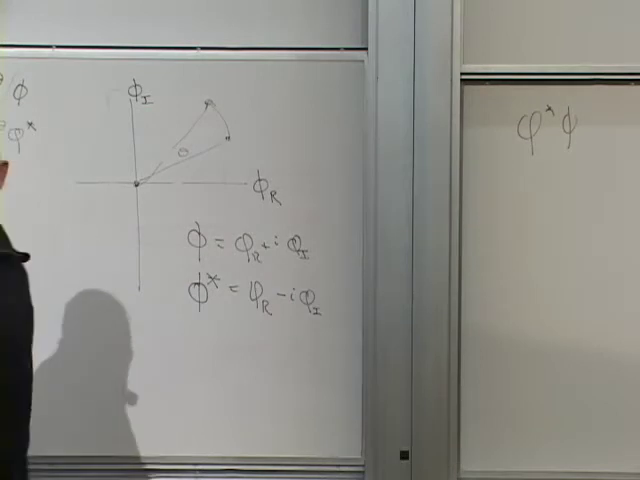
\includegraphics[width=0.80\textwidth]{lecture_07_figure_02.png}
\caption{El campo complejo en el plano interno \((\phi_R,\phi_I)\). La pizarra muestra la descomposición de \(\phi\) y \(\phi^*\), y el radio invariante \(\phi^*\phi\).}
\lectureframe{00:33:33}
\end{figure}

Tomemos el lagrangiano
\begin{equation}
  \mathcal L
  =\partial_\mu\phi^*\,\partial^\mu\phi
   -V(\phi^*\phi).
  \label{eq:l07-complex-lagrangian}
\end{equation}
Para un campo complejo se omite el factor convencional \(1/2\), porque este único producto ya contiene los términos cinéticos de ambas componentes reales. La transformación
\begin{equation}
  \phi'(x)=e^{i\theta}\phi(x),
  \qquad
  \phi^{*\prime}(x)=e^{-i\theta}\phi^*(x)
  \label{eq:l07-global-u1}
\end{equation}
rota por el mismo ángulo todos los valores del campo. Aquí \(\theta\) es constante en el espacio y el tiempo. La prima indica el campo transformado; no es una derivada.

Como \(\theta\) es constante,
\begin{equation}
  \partial_\mu\phi'=e^{i\theta}\partial_\mu\phi,
  \qquad
  \partial_\mu\phi^{*\prime}
  =e^{-i\theta}\partial_\mu\phi^*.
\end{equation}
Las fases se cancelan en el término cinético, y
\(\phi^{*\prime}\phi'=\phi^*\phi\). Así, todo potencial que dependa únicamente de \(\phi^*\phi\) tiene la misma simetría. Un término que dependiera solo de \(\phi_R\) seleccionaría una dirección en el plano interno y la rompería explícitamente.

\subsection{Un mínimo puntual y un círculo de mínimos}

Hay dos tipos cualitativamente distintos de potenciales simétricos. El primero tiene su único mínimo en el origen; por ejemplo,
\begin{equation}
  V_{\rm unbroken}=m^2\phi^*\phi,
  \qquad m^2>0.
\end{equation}
Su gráfica es un paraboloide con simetría rotacional. El vacío \(\phi=0\) permanece fijo bajo toda rotación, así que la simetría no está rota.

Elijamos ahora
\begin{equation}
  V_{\rm broken}
  =-a\,\phi^*\phi+b(\phi^*\phi)^2,
  \qquad a,b>0.
  \label{eq:l07-mexican-hat}
\end{equation}
El término cuadrático negativo empuja el campo para alejarlo del origen, mientras que el término cuártico positivo impide que se dispare hasta el infinito. Si escribimos \(r^2=\phi^*\phi\), la minimización da
\begin{equation}
  \frac{dV}{d(r^2)}=-a+2br^2=0,
  \qquad
  r^2=f^2=\frac{a}{2b}.
  \label{eq:l07-vacuum-radius}
\end{equation}
Por tanto, los mínimos forman un círculo. El potencial tiene simetría rotacional perfecta, pero un estado fundamental uniforme debe elegir un punto de ese círculo.

\begin{figure}[htbp]
\centering
\includegraphics[width=0.72\textwidth]{lecture_07_figure_06.png}
\caption{El potencial que rompe la simetría, dibujado como una superficie de revolución. El origen es inestable y los mínimos degenerados forman el fondo circular.}
\lectureframe{00:37:25}
\end{figure}

Imaginemos que en cada punto del espacio ordinario el campo es una pequeña flecha en este plano interno. El potencial exige que cada flecha tenga longitud \(f\). La energía del gradiente exige que las flechas cercanas apunten casi en la misma dirección. En consecuencia, el estado fundamental tiene el mismo ángulo en todas partes, pero la ley no prefiere ninguno. Eso es la ruptura espontánea de una simetría continua.

\section{De una pared de dominio a un giro suave}

Repitamos el experimento con los contornos. En el contorno izquierdo fijemos el campo en un punto de vacío \(A\); en el derecho, en otro punto de vacío \(B\). Un salto localizado haría que el gradiente fuera grande. Sin embargo, a diferencia del caso discreto, el campo puede permanecer en el fondo del potencial mientras cambia continuamente alrededor del círculo.

A baja energía, escribamos el campo como \(\phi=f e^{i\alpha(x)}\). En una dimensión espacial, la energía relevante es
\begin{equation}
  E[\alpha]
  =f^2\int_0^L dx\,\left(\frac{d\alpha}{dx}\right)^2.
  \label{eq:l07-angle-functional}
\end{equation}
Para ángulos extremos fijos, la variación da
\begin{equation}
  \frac{d^2\alpha}{dx^2}=0,
  \qquad
  \alpha(x)=\alpha_A+
    \frac{\alpha_B-\alpha_A}{L}\,x.
  \label{eq:l07-linear-twist}
\end{equation}
La configuración preferida distribuye el giro uniformemente por toda la muestra. Su energía escala como
\begin{equation}
  E_{\rm twist}
  =f^2\frac{(\alpha_B-\alpha_A)^2}{L},
  \label{eq:l07-twist-energy}
\end{equation}
por lo que puede hacerse arbitrariamente pequeña al aumentar \(L\).

\begin{figure}[htbp]
\centering
\begin{adjustbox}{max width=\linewidth}
\begin{tikzpicture}[x=0.95cm,y=0.95cm]
  \begin{scope}
    \draw[->] (0,0) -- (6.2,0) node[right] {$x$};
    \draw[->] (0,0) -- (0,3.5) node[above] {$\alpha(x)$};
    \draw[very thick,blue!70!black] (0.45,0.65) -- (5.7,2.85);
    \fill (0.45,0.65) circle (1.8pt) node[left] {$\alpha_A$};
    \fill (5.7,2.85) circle (1.8pt) node[right] {$\alpha_B$};
    \node at (3.1,-0.65) {physical space};
  \end{scope}
  \begin{scope}[xshift=9.2cm,yshift=1.65cm]
    \draw[thick] (0,0) circle (1.8);
    \fill (1.55,-0.92) circle (1.8pt) node[below right] {$A$};
    \fill (-0.45,1.74) circle (1.8pt) node[above] {$B$};
    \draw[very thick,blue!70!black,-{Latex[length=2.5mm]}]
      (1.55,-0.92) arc[start angle=-31,end angle=104,radius=1.8];
    \node at (0,-2.35) {vacuum circle};
  \end{scope}
\end{tikzpicture}
\end{adjustbox}
\caption{La misma configuración de baja energía en dos descripciones. El ángulo varía linealmente a través del espacio físico, mientras que el campo sigue el arco corto del círculo de vacío en el espacio interno.}
\end{figure}

\begin{classroomqa}
\audiencequestion{Hay dos maneras de recorrer el círculo. ¿Qué camino sigue el campo y puede quedar atrapado en el más largo?
\lecturetimestamp{00:41:54}}
\lecturerresponse{Para extremos genéricos, la ruta angular más corta tiene un gradiente menor y, por tanto, menor energía. Si los extremos son diametralmente opuestos, las dos rutas más sencillas son degeneradas. Una configuración preparada moviendo lentamente uno de los extremos puede conservar un número de vueltas adicional y quedar atrapada tras una barrera de energía; pero, para un par determinado de extremos ordinarios, la ruta más corta sin torsión es el estado fundamental.}
\end{classroomqa}

\begin{classroomqa}
\audiencequestion{¿Podría el camino salir del fondo del valle y atravesar el interior, acortándose en conjunto?
\lecturetimestamp{00:43:32}}
\lecturerresponse{En el régimen de baja energía y muestras largas, no compensa subir por el potencial radial. Mantener el radio en su valor de vacío y variar el ángulo linealmente minimiza la energía efectiva, como muestra el cálculo variacional anterior. En un sistema finito con un potencial específico se pueden minimizar conjuntamente el movimiento radial y el angular, pero la conclusión de Goldstone se refiere al límite de longitudes de onda arbitrariamente grandes, en el que prevalece el movimiento suave a lo largo del valle.}
\end{classroomqa}

\begin{classroomqa}
\audiencequestion{¿Qué cambia si se inclina el valle circular para que un ángulo tenga menor energía?
\lecturetimestamp{00:44:33}}
\lecturerresponse{Entonces la simetría se rompe explícitamente. Un punto se convierte en el verdadero estado fundamental, el movimiento a lo largo del círculo adquiere una fuerza restauradora y la excitación angular deja de ser exactamente sin masa.}
\end{classroomqa}

\section{La masa como costo de una oscilación con momento nulo}

El giro suave revela un campo cuya energía procede únicamente de los gradientes. Para entender por qué eso implica una partícula sin masa, comparemos la relación de dispersión relativista
\begin{equation}
  \omega^2=\bm{k}^2+m^2.
  \label{eq:l07-dispersion}
\end{equation}
Una onda \(e^{i(\bm{k}\cdot\bm{x}-\omega t)}\) lleva momento \(\bm{k}\).
Si \(m=0\), su energía tiende a cero cuando la longitud de onda tiende al infinito:
\(\omega=|\bm{k}|\to0\). Si \(m\ne0\), un modo espacialmente homogéneo \(\bm{k}=0\) sigue oscilando con frecuencia \(\omega=m\). La masa es la energía irreducible con momento nulo.

Esta misma distinción se observa en el lagrangiano. Un término
\begin{equation}
  -\frac12m^2\varphi^2
\end{equation}
aporta una fuerza restauradora incluso para un desplazamiento homogéneo. Un campo que solo tiene términos con derivadas carece de esa fuerza restauradora: al aumentar la longitud de onda, su energía de gradiente se aproxima a cero.

\subsection{Las variables polares separan los dos modos}

Escribamos el campo complejo con simetría rota como
\begin{equation}
  \phi(x)=\rho(x)e^{i\alpha(x)}.
  \label{eq:l07-polar}
\end{equation}
Tanto \(\rho\) como \(\alpha\) son campos. Al derivar se obtiene
\begin{align}
  \partial_\mu\phi
  &=e^{i\alpha}
    \left(\partial_\mu\rho+i\rho\,\partial_\mu\alpha\right),\\
  \partial_\mu\phi^*
  &=e^{-i\alpha}
    \left(\partial_\mu\rho-i\rho\,\partial_\mu\alpha\right).
\end{align}
Los términos cruzados se cancelan y queda
\begin{equation}
  \partial_\mu\phi^*\,\partial^\mu\phi
  =(\partial_\mu\rho)(\partial^\mu\rho)
   +\rho^2(\partial_\mu\alpha)(\partial^\mu\alpha).
  \label{eq:l07-polar-kinetic}
\end{equation}
Como \(\phi^*\phi=\rho^2\),
\begin{equation}
  \mathcal L
  =(\partial\rho)^2+\rho^2(\partial\alpha)^2-V(\rho^2).
  \label{eq:l07-polar-lagrangian}
\end{equation}
El potencial contiene \(\rho\), pero no \(\alpha\). Esa ausencia expresa la simetría en su forma más útil.

\begin{figure}[htbp]
\centering
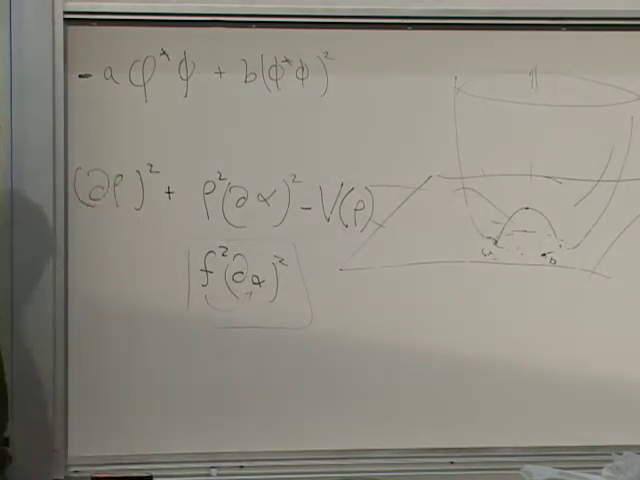
\includegraphics[width=0.88\textwidth]{lecture_07_figure_03.png}
\caption{El lagrangiano en variables polares, su término angular de baja energía enmarcado y el potencial que rompe la simetría. El movimiento radial hace subir por el potencial; el angular sigue el valle.}
\lectureframe{00:56:40}
\end{figure}

Para una excitación de energía muy baja, el campo permanece cerca de \(\rho=f\). Entonces
\begin{equation}
  \mathcal L_{\rm angular}
  \simeq f^2(\partial_\mu\alpha)(\partial^\mu\alpha).
\end{equation}
Definamos el campo angular con normalización canónica, salvo la convención para los factores de \(1/2\), mediante
\begin{equation}
  \beta=\sqrt{2}\,f\alpha,
  \qquad
  \mathcal L_{\rm angular}
  =\frac12(\partial_\mu\beta)(\partial^\mu\beta).
  \label{eq:l07-goldstone-field}
\end{equation}
No hay término \(\beta^2\). Los cuantos de este campo angular no tienen masa. Son los bosones de Goldstone.

El campo radial se comporta de otra manera. Si desplazamos \(\rho\) de \(f\) en todas partes a la vez, rueda de vuelta, sobrepasa el mínimo y oscila alrededor del fondo del valle. Si \(\rho=f+h\), el desarrollo de la Ec.~\eqref{eq:l07-mexican-hat} produce
\begin{equation}
  V(f+h)=V(f)+\frac12m_h^2h^2+\cdots,
\end{equation}
por lo que \(h\) tiene masa. Geométricamente, la dirección angular es plana y la radial es curva.

\begin{classroomqa}
\audiencequestion{Si el campo se desplaza radialmente, ¿simplemente vuelve a bajar? ¿Qué ocurre después?\lecturetimestamp{00:57:10}}
\lecturerresponse{Sin movimiento angular, cae hacia el mínimo, lo sobrepasa y oscila radialmente. Una oscilación homogénea tiene momento espacial nulo, pero frecuencia distinta de cero; esa frecuencia es la masa de la excitación radial. En cambio, un desplazamiento angular homogéneo termina en otro vacío y no tiene fuerza restauradora.}
\end{classroomqa}

Este es el contenido del principio de Goldstone en el ejemplo actual: la ruptura espontánea de una simetría global continua produce un modo sin masa por cada dirección plana independiente de la variedad de vacíos.
\editorialnote{El enunciado supone las condiciones habituales de la teoría relativista de campos. En sistemas de muchos cuerpos no relativistas, el recuento y la dispersión de los modos de Nambu--Goldstone pueden ser más sutiles, pero la conclusión de la lección sobre longitudes de onda largas sigue siendo válida para este modelo relativista \(U(1)\).}

\section{Ondas de espín, cuerdas y sonido}

El teorema es abstracto, pero su mecanismo resulta familiar. En un ferromagneto isotrópico, se pueden rotar todos los espines juntos sin cambiar la energía. Si la orientación varía muy lentamente a través de la muestra, se obtiene una onda de espín. Su costo se anula al tender a cero el número de onda, así que es el modo de Goldstone de la simetría rota por rotaciones de espín.

Una cuerda elástica larga ofrece otra imagen. Ignorando la gravedad, montemos los extremos de modo que se pueda trasladar verticalmente toda la cuerda. Una traslación vertical uniforme no cuesta energía. Si hacemos que la traslación varíe lentamente a lo largo de la cuerda, se convierte en una onda transversal de longitud de onda larga. La operación de simetría uniforme se ha convertido en una deformación suave que depende de la posición.

\begin{figure}[htbp]
\centering
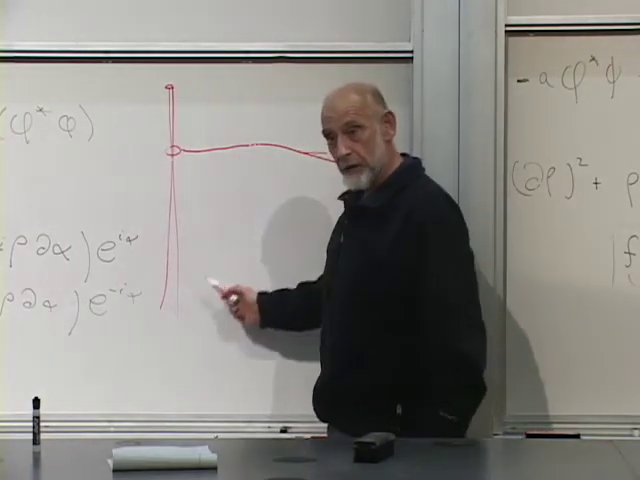
\includegraphics[width=0.68\textwidth]{lecture_07_figure_04.png}
\caption{El perfil de la cuerda que varía lentamente, dibujado durante la analogía con el modo de Goldstone. Lo importante físicamente es la pequeña pendiente de una deformación de longitud de onda larga, no la posición vertical de la curva.}
\lectureframe{01:04:19}
\end{figure}

\begin{classroomqa}
\audiencequestion{¿Puede la cuerda transportar energía de oscilación y tener momento nulo?
\lecturetimestamp{01:04:41}}
\lecturerresponse{Hay que distinguir el momento mecánico vertical del momento de onda a lo largo de la cuerda. Una onda estacionaria puede tener momento neto nulo porque es una superposición de modos con \(+k\) y \(-k\), y aun así transportar energía. En la analogía con la teoría de campos, el momento se refiere al número de onda a lo largo del eje; el desplazamiento vertical representa la coordenada interna del campo.}
\end{classroomqa}

Un muelle extensible ilustra la versión longitudinal. Traslademos todo el muelle infinito idealizado a lo largo de su eje: nada cambia. Si trasladamos las partes vecinas en cantidades ligeramente distintas, el resultado es una onda de compresión suave. En un sólido o un fluido, el sonido de longitud de onda larga surge de desplazamientos colectivos y variaciones de densidad. Las ondas de espín, las ondas transversales en una cuerda y el sonido no son la misma excitación microscópica, pero comparten el patrón decisivo: una operación continua uniforme no cuesta energía, y su versión que varía lentamente se convierte en un modo blando.
\editorialnote{En un cristal, los fonones acústicos se describen convencionalmente como modos de Nambu--Goldstone asociados a la ruptura espontánea de las traslaciones continuas. La cuerda y el muelle extensible son analogías mecánicas que se usan en la lección para mostrar la misma estructura de energía que depende únicamente de derivadas.}

La terminología merece una breve broma de clase: son bosones de \emph{Goldstone}, llamados así por Jeffrey Goldstone, no bosones gauge. La lección señala que Goldstone era amigo de Susskind y luego pasa al tema realmente distinto de la invariancia gauge.

\section{De la simetría global de fase a la simetría gauge}

La simetría de fase \(U(1)\) ya apareció en el curso como la simetría asociada a la conservación de la carga. Los campos de partículas cargadas son complejos, y multiplicarlos por una fase común deja inalterada la teoría global. Se puede hablar de carga eléctrica para facilitar la intuición, aunque la carga podría representar otro número cuántico \(U(1)\). El fotón real no tiene masa; el objetivo final es un campo similar al fotón, como el \(Z\) masivo.

La nueva pregunta es si
\begin{equation}
  \phi'(x)=e^{i\theta(x)}\phi(x)
  \label{eq:l07-local-u1}
\end{equation}
puede ser una simetría cuando \(\theta\) varía arbitrariamente por el espacio-tiempo. La función \(\theta(x)\) es un parámetro de transformación, no un campo dinámico adicional. Comprobemos la propuesta derivando:
\begin{equation}
  \partial_\mu\phi'
  =e^{i\theta}
   \left[\partial_\mu\phi+i(\partial_\mu\theta)\phi\right].
  \label{eq:l07-local-derivative}
\end{equation}
El término adicional no aparecía cuando \(\theta\) era constante. Para el conjugado,
\begin{equation}
  \partial_\mu\phi^{*\prime}
  =e^{-i\theta}
   \left[\partial_\mu\phi^*-i(\partial_\mu\theta)\phi^*\right].
\end{equation}
El producto es
\begin{align}
  \partial_\mu\phi^{*\prime}\partial^\mu\phi'
  ={}&
  \partial_\mu\phi^*\partial^\mu\phi
  i\left(
      \phi\,\partial_\mu\phi^*
      -\phi^*\partial_\mu\phi
    \right)\partial^\mu\theta
  \nonumber\\
  &+\phi^*\phi\,
    \partial_\mu\theta\,\partial^\mu\theta.
  \label{eq:l07-local-failure}
\end{align}
El potencial sigue siendo invariante porque también lo es \(\phi^*\phi\), pero el término cinético ordinario no lo es. Una simetría global no se convierte automáticamente en una simetría local.

\begin{classroomqa}
\audiencequestion{En la imagen del sombrero mexicano, ¿este fallo significa que hay bultos alrededor del valle circular?
\lecturetimestamp{01:19:37}}
\lecturerresponse{No. El potencial puede seguir siendo perfectamente plano en la dirección angular. El costo adicional proviene de los gradientes cuando la fase difiere entre distintos puntos del espacio-tiempo. No se trata de ondulaciones del valle: es el término ordinario de derivadas que detecta la variación espacial.}
\end{classroomqa}

\subsection{El campo vectorial compensador}

Las interacciones del fotón de la naturaleza, \(W\), \(Z\) y los gluones están organizadas por simetrías gauge locales, no solo por transformaciones rígidas. Para que la operación de fase local sea una simetría, ampliemos la teoría con un campo de cuatro vectores \(A_\mu\). En electromagnetismo, \(A_0\) es el potencial escalar y las tres componentes espaciales forman el potencial vector. Sus derivadas construyen los campos eléctrico y magnético.

Elijamos una convención internamente consistente:
\begin{equation}
  \phi'=e^{i\theta}\phi,
  \qquad
  A'_\mu=A_\mu-\partial_\mu\theta,
  \qquad
  D_\mu=\partial_\mu+iA_\mu.
  \label{eq:l07-gauge-convention}
\end{equation}
Al comprobar la cancelación, en la pizarra se cambia un signo; la Ec.
\eqref{eq:l07-gauge-convention}
fija conjuntamente los tres signos. Por ahora, las constantes de acoplamiento y de carga se han absorbido en \(A_\mu\).
\editorialnote{Con la carga explícita \(q\) y el acoplamiento \(g\), se puede escribir \(D_\mu=\partial_\mu+igqA_\mu\) y
\(A'_\mu=A_\mu-(gq)^{-1}\partial_\mu\theta\). La lección omite estas constantes para que la cancelación quede a la vista.}

Para el campo conjugado,
\begin{equation}
  D_\mu\phi^*=\partial_\mu\phi^*-iA_\mu\phi^*.
\end{equation}
Ahora bien,
\begin{align}
  D'_\mu\phi'
  &=
  \left(\partial_\mu+iA'_\mu\right)e^{i\theta}\phi
  \nonumber\\
  &=
  e^{i\theta}
  \left[
    \partial_\mu\phi+i(\partial_\mu\theta)\phi
    +i(A_\mu-\partial_\mu\theta)\phi
  \right]
  \nonumber\\
  &=e^{i\theta}D_\mu\phi.
  \label{eq:l07-covariant-transform}
\end{align}
La transformación de \(A_\mu\) cancela la derivada no deseada de \(\theta\). Asimismo,
\begin{equation}
  D'_\mu\phi^{*\prime}=e^{-i\theta}D_\mu\phi^*.
\end{equation}
Su producto es invariante. El adjetivo \emph{covariante} significa que la derivada se transforma de la misma manera sencilla que el propio campo.

\section{Dinámica del campo gauge}

Introducir \(A_\mu\) solo para reparar una derivada lo dejaría sin dinámica propia. El tensor de campo gauge invariante es
\begin{equation}
  F_{\mu\nu}
  =\partial_\mu A_\nu-\partial_\nu A_\mu.
  \label{eq:l07-field-strength}
\end{equation}
Es antisimétrico, por lo que \(F_{\mu\mu}=0\). Sus componentes tiempo--espacio contienen el campo eléctrico, mientras que sus componentes espacio--espacio contienen el campo magnético. En el lenguaje familiar de los vectores tridimensionales, la densidad de energía electromagnética es proporcional a \(\bm E^2+\bm B^2\), mientras que el lagrangiano lorentziano es proporcional a \(\bm E^2-\bm B^2\), con signos que dependen de la convención de métrica.

\begin{classroomqa}
\audiencequestion{¿Cuáles son la energía y el lagrangiano del campo electromagnético?\lecturetimestamp{01:33:20}}
\lecturerresponse{La energía se construye a partir de \(E^2+B^2\); el lagrangiano usa \(E^2-B^2\). En forma covariante, este último se escribe como un múltiplo convencional de \(F_{\mu\nu}F^{\mu\nu}\). El tensor antisimétrico es el rotacional cuatridimensional del potencial vector.}
\end{classroomqa}

El tensor de campo es invariante gauge por sí mismo:
\begin{align}
  F'_{\mu\nu}
  &=
  \partial_\mu(A_\nu-\partial_\nu\theta)
  -\partial_\nu(A_\mu-\partial_\mu\theta)
  \nonumber\\
  &=
  F_{\mu\nu}
  -\partial_\mu\partial_\nu\theta
  +\partial_\nu\partial_\mu\theta
  =F_{\mu\nu}.
  \label{eq:l07-field-strength-invariant}
\end{align}
La igualdad final se sigue de que las derivadas parciales mixtas ordinarias conmutan. Por tanto, un lagrangiano gauge invariante estándar es
\begin{equation}
  \boxed{
  \mathcal L
  =(D_\mu\phi)^*D^\mu\phi
  -V(\phi^*\phi)
  -\frac14F_{\mu\nu}F^{\mu\nu}}
  \label{eq:l07-scalar-qed}
\end{equation}
hasta el signo y la normalización elegidos para la métrica.

\begin{figure}[htbp]
\centering
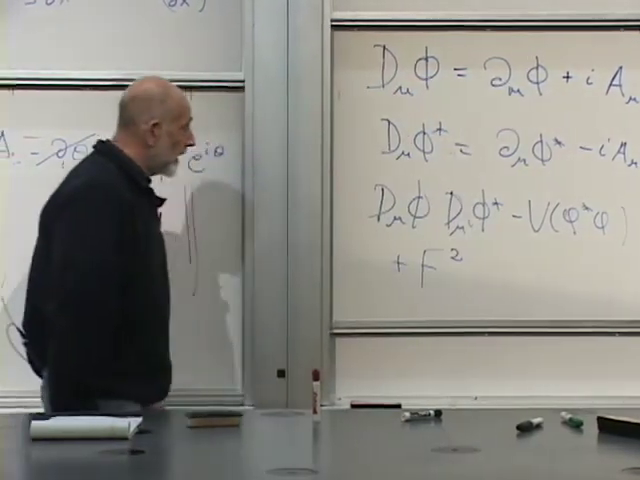
\includegraphics[width=0.84\textwidth]{lecture_07_figure_05.png}
\caption{Las derivadas covariantes y el lagrangiano gauge invariante completo, tal como aparecen en la pizarra. Allí se omiten los factores numéricos para que la estructura de las transformaciones siga siendo visible.}
\lectureframe{01:38:45}
\end{figure}

Esta construcción convierte una simetría global \(U(1)\) en una local, pero lo hace a costa---o, físicamente, a cambio---de introducir un nuevo campo vectorial. En el ejemplo abeliano, ese campo es el potencial electromagnético.

\begin{classroomqa}
\audiencequestion{El lagrangiano con el que empezamos usaba derivadas ordinarias. ¿Por qué podemos sustituirlas por derivadas covariantes y llamar al resultado la teoría real?\lecturetimestamp{01:42:55}}
\lecturerresponse{Estamos construyendo una teoría distinta y ampliada: materia cargada más un campo gauge. La invariancia gauge local determina su acoplamiento. La teoría cuántica resultante es una estructura matemática coherente y concuerda con la manera en que la naturaleza organiza los campos gauge del fotón y de la interacción débil. Acoplar sin coherencia un campo vectorial relativista puede introducir polarizaciones no físicas y violaciones de la probabilidad, así que el principio gauge no es una mera reformulación cosmética de la antigua teoría escalar libre.}
\end{classroomqa}

\begin{classroomqa}
\audiencequestion{Así que añadir el nuevo campo es la justificación esencial de la modificación?\lecturetimestamp{01:44:57}}
\lecturerresponse{Sí. Sin \(A_\mu\), la derivada de un campo rotado localmente contiene un término \(\partial_\mu\theta\) que no se cancela. Con \(A_\mu\) y su ley de transformación, la cancelación funciona. En lenguaje geométrico, \(A_\mu\) es una conexión en un fibrado; esas matemáticas más profundas son reales y útiles, pero el álgebra anterior contiene lo necesario aquí.}
\end{classroomqa}

\section{Por qué está prohibida una masa desnuda para un bosón gauge}

Para un campo bosónico ordinario, la masa se representa mediante un término cuadrático. Resulta tentador añadir
\begin{equation}
  \Delta\mathcal L_{\rm Proca}
  =\frac12m^2A_\mu A^\mu.
  \label{eq:l07-proca}
\end{equation}
Pero bajo \(A_\mu\mapsto A_\mu-\partial_\mu\theta\),
\begin{equation}
  A'_\mu A^{\mu\prime}
  =
  A_\mu A^\mu
  -2A^\mu\partial_\mu\theta
  +\partial_\mu\theta\,\partial^\mu\theta,
\end{equation}
por lo que la ecuación~\eqref{eq:l07-proca} no es invariante gauge. No podemos introducir a mano una masa en esta teoría gauge y conservar al mismo tiempo su simetría local.

\begin{figure}[htbp]
\centering
\includegraphics[width=0.72\textwidth]{lecture_07_figure_07.png}
\caption{La masa vectorial desnuda propuesta
\(\tfrac12m^2A_\mu A^\mu\). Su falta de invariancia bajo
\(A_\mu\mapsto A_\mu-\partial_\mu\theta\) es el obstáculo que prepara el terreno para el mecanismo de Higgs.}
\lectureframe{01:39:48}
\end{figure}

Este es el aparente callejón sin salida. La invariancia gauge explica que el fotón no tenga masa y protege la teoría de grados de libertad no físicos, pero \(W\) y \(Z\) tienen masa. La salida no puede consistir en añadir explícitamente una masa vectorial. Debe surgir de los campos que ya están presentes en un lagrangiano invariante gauge.

\begin{classroomqa}
\audiencequestion{¿La introducción de la invariancia gauge produce por sí misma el bosón de Goldstone?\lecturetimestamp{01:45:51}}
\lecturerresponse{No. El bosón de Goldstone surgió cuando se rompió espontáneamente una simetría \emph{global} continua, antes de introducir el potencial vectorial. Una vez que la simetría es local, \(A_\mu\) puede compensar una fase variable. En la teoría gauge rota, el modo angular deja de ser una partícula independiente sin masa; proporciona la polarización adicional del campo vectorial, que ahora tiene masa. En la próxima conferencia deduciremos esta afirmación en lugar de limitarnos a enunciarla.}
\end{classroomqa}

\begin{classroomqa}
\audiencequestion{¿Explica algo de esto por qué los ríos serpentean?
\lecturetimestamp{01:47:03}}
\lecturerresponse{Aquí no se conoce ninguna conexión directa. Los remolinos de los fluidos e incluso las formas de los organismos pueden describirse sin duda mediante métodos de simetría, y nunca debería sorprendernos encontrar ideas de teoría de campos en lugares inesperados, pero en la conferencia no se propone ninguna teoría gauge de los meandros fluviales.}\end{classroomqa}

\section{Dónde termina la conferencia}

Ya tenemos los dos ingredientes prometidos al principio. Una simetría global continua con un círculo de vacíos tiene una dirección angular plana, y su variación lenta es un campo de Goldstone sin masa. Una simetría local requiere una conexión gauge y derivadas covariantes, y prohíbe la masa vectorial directa de la ecuación~\eqref{eq:l07-proca}.

El siguiente paso consiste en usar el potencial roto de la ecuación~\eqref{eq:l07-mexican-hat} dentro de la teoría invariante gauge de la ecuación~\eqref{eq:l07-scalar-qed}. Entonces ocurren dos cosas a la vez: la partícula de Goldstone deja de aparecer como partícula independiente en el espectro físico, y el campo vectorial adquiere masa. En el lenguaje pedagógico habitual, se dice que la simetría gauge se rompe espontáneamente; con mayor precisión, la redundancia gauge permanece mientras la teoría entra en una fase de Higgs con una excitación vectorial masiva.
\editorialnote{Una simetría gauge local es una redundancia de la descripción, no una simetría física ordinaria que actúe entre estados observables distintos. La conferencia emplea la expresión abreviada habitual «ruptura espontánea de la simetría gauge». La afirmación física invariante gauge es la reorganización de los grados de libertad en la fase de Higgs.}

Ese es el fenómeno de Higgs. Todavía no lo hemos llevado a cabo. Esta conferencia ha hecho el trabajo, más difícil pero necesario, de precisar el problema lo suficiente para que la solución, cuando llegue, sea inevitable.

\chapter{El mecanismo de Higgs: cómo adquiere masa un bosón gauge}

Ahora reunimos las dos ideas desarrolladas en la clase anterior. Un campo escalar complejo con una simetría global \(U(1)\) rota contiene una oscilación radial masiva y una oscilación angular sin masa. Una teoría localmente invariante bajo \(U(1)\) contiene un campo gauge sin masa. Cuando el escalar está cargado y su magnitud de equilibrio es distinta de cero, estas afirmaciones no pueden simplemente combinarse. El modo angular y el campo gauge se combinan: el campo gauge adquiere masa, el bosón de Goldstone aparente deja de ser una partícula independiente y permanece el modo radial de Higgs.

Tomaremos el fotón como modelo de bosón gauge, pero no como conclusión física. La simetría electromagnética \(U(1)\) no está rota en el vacío, así que el fotón real no tiene masa. El mismo mecanismo actúa sobre \(W^\pm\) y \(Z\) en la teoría electrodébil, donde el grupo gauge y el multiplete escalar son más complicados. El modelo abeliano permite ver el mecanismo sin ocultarlo bajo la teoría de grupos.

\begin{classroomqa}
\audiencequestion{¿La explicación anterior quería decir que el mecanismo de Higgs da masa al fotón real?\lecturetimestamp{00:00:23}}
\lecturerresponse{No. Preguntamos qué ocurriría \emph{si} el \(U(1)\) asociado al fotón estuviera en una fase rota. Ese fotón hipotético adquiriría masa. El vacío electromagnético real no está en esa fase; en física de partículas, la aplicación del mecanismo es, en cambio, la masa de \(W\) y \(Z\).}
\end{classroomqa}

La simetría asociada a la conservación de la carga eléctrica es la rotación de fase
\begin{equation}
  \phi(x)\longmapsto e^{i\theta}\phi(x),
\end{equation}
una rotación interna llamada \(U(1)\). Un superconductor proporciona una analogía real de la fase rota. En su interior, el campo electromagnético tiene una profundidad de penetración finita y, en aspectos importantes, se comporta como un campo masivo. En el exterior reaparece el fotón ordinario sin masa.

\section{Qué significa la masa para un campo}

\subsection{Dispersión y brecha en el momento nulo}

Conviene precisar qué entendemos por masa antes de introducir el campo de Higgs. Para una onda,
\begin{equation}
  E=\hbar\omega,
  \qquad
  p=\hbar k,
  \label{eq:l08-quantum-wave}
\end{equation}
así que las gráficas \((E,p)\) y \((\omega,k)\) contienen la misma información, salvo por factores de \(\hbar\). En el espacio vacío, una excitación relativista sin masa satisface
\begin{equation}
  E=c|p|,
  \qquad
  \omega=c|k|.
  \label{eq:l08-massless-dispersion}
\end{equation}
Los dos signos de \(k\) distinguen sentidos de propagación opuestos. Lo esencial es que \(\omega\) tiende a cero cuando lo hace \(k\).

Una partícula relativista masiva satisface
\begin{equation}
  E^2=c^2p^2+m^2c^4.
  \label{eq:l08-massive-dispersion}
\end{equation}
En unidades \(c=\hbar=1\),
\begin{equation}
  \omega^2=k^2+m^2.
\end{equation}
En \(k=0\), la energía es \(E=mc^2\), o simplemente \(m\) en unidades naturales. Por tanto, la masa es la brecha de energía distinta de cero del modo con momento nulo.

\begin{figure}[htbp]
\centering
\begin{adjustbox}{max width=\linewidth}
\begin{tikzpicture}[x=1.05cm,y=1.05cm]
  \begin{scope}
    \draw[->] (-0.2,0) -- (4.2,0) node[right] {\(k\)};
    \draw[->] (0,-0.2) -- (0,3.1) node[above] {\(\omega\)};
    \draw[very thick,blue!65!black] (0,0) -- (3.8,2.75);
    \draw[very thick,orange!70!black] (0,0) -- (3.8,1.75);
    \node[blue!65!black,rotate=36] at (2.65,2.15)
      {\(\omega=c_{\rm vac}k\)};
    \node[orange!70!black,rotate=24] at (2.65,1.05)
      {ordinary medium};
    \node[below] at (2,-0.45) {gapless};
  \end{scope}
  \begin{scope}[xshift=6.2cm]
    \draw[->] (-0.2,0) -- (4.2,0) node[right] {\(k\)};
    \draw[->] (0,-0.2) -- (0,3.1) node[above] {\(\omega\)};
    \draw[very thick,domain=0:3.8,samples=120,smooth,teal!70!black]
      plot (\x,{sqrt(0.9+0.45*\x*\x)});
    \draw[dashed] (0,0.95) -- (1.0,0.95);
    \node[left] at (0,0.95) {\(m\)};
    \node[teal!70!black] at (2.55,2.15)
      {\(\omega^2=k^2+m^2\)};
    \node[below] at (2,-0.45) {gapped};
  \end{scope}
\end{tikzpicture}
\end{adjustbox}
\caption{Cambiar la velocidad de propagación modifica la pendiente de una relación de dispersión sin brecha. Dar masa a la excitación abre una brecha distinta de cero en \(k=0\).}
\label{fig:l08-dispersion}
\end{figure}

Un material transparente ordinario puede reducir la velocidad de fase de una onda sin crear esta brecha de masa relativista. En una interfaz, la frecuencia incidente se mantiene fija, mientras que el número de onda se ajusta a la relación de dispersión del medio. Cambiar la pendiente no equivale a elevar la ordenada al origen.
\editorialnote{Un material puede tener varias ramas electromagnéticas, y un plasma o un medio resonante puede presentar una brecha distinta de cero asociada a la frecuencia de plasma. La comparación de esta clase se refiere específicamente a una rama refractiva ordinaria y a la respuesta superconductora. En términos más generales, que no haya brecha significa que \(\omega(k)\to0\) cuando \(k\to0\); no se requiere una relación lineal exacta en todos los medios no relativistas.}

\begin{classroomqa}
\audiencequestion{¿Adquiere masa un fotón cada vez que atraviesa la materia, por ejemplo, un prisma?\lecturetimestamp{00:03:02}}
\lecturerresponse{No. La refracción puede cambiar la relación entre la frecuencia y el número de onda y, por tanto, la velocidad de propagación, aunque la rama siga pasando por \(\omega=0\) en \(k=0\). En cambio, una fase superconductora confiere a la respuesta electromagnética una longitud inversa de penetración finita, análoga a una masa.}
\end{classroomqa}

\begin{classroomqa}
\audiencequestion{Cuando la luz de frecuencia fija entra en el vidrio, ¿cambia el número de onda?\lecturetimestamp{00:09:20}}
\lecturerresponse{Sí. La invariancia ante traslaciones temporales en una interfaz estacionaria mantiene fija la frecuencia. Como la curva de dispersión tiene una pendiente distinta en el vidrio, el mismo \(\omega\) corresponde a un \(k\) distinto y, por tanto, a una longitud de onda diferente.}
\end{classroomqa}

La pendiente
\begin{equation}
  v_g=\frac{d\omega}{dk}
\end{equation}
es la velocidad de grupo de un paquete de ondas. Si esa pendiente varía con \(k\), las distintas componentes de Fourier se desplazan a velocidades diferentes y el paquete se dispersa. Por eso la relación \(\omega(k)\) se llama relación de \emph{dispersión}.

\begin{classroomqa}
\audiencequestion{¿Cómo se llama la curva y qué representa su pendiente?\lecturetimestamp{00:11:02}}
\lecturerresponse{La curva es la relación de dispersión. Su derivada \(d\omega/dk\) es la velocidad de grupo. Una pendiente constante da la misma velocidad a todas las longitudes de onda; si la pendiente varía, el paquete de ondas se ensancha. Para lo que nos ocupa, la distinción decisiva es si la curva alcanza el origen o tiene una brecha.}
\end{classroomqa}

\subsection{Una oscilación homogénea es una partícula en reposo}

El modo \(k=0\) tiene longitud de onda infinita: el campo está desplazado en la misma cantidad en todas partes. Liberemos un desplazamiento homogéneo. Si el campo oscila con una frecuencia distinta de cero, el cuanto correspondiente tiene energía en reposo distinta de cero y es masivo. Si en esa dirección no hay fuerza restauradora, la frecuencia se anula y el modo no tiene masa.

Esta afirmación es clásica. No requiere que partículas separadas espacialmente estén en una superposición cuántica. Una configuración clásica homogénea del campo consiste simplemente en un mismo valor del campo repetido por todo el espacio.

\begin{classroomqa}
\audiencequestion{Si se desplaza todo un campo a la vez, ¿es eso lo mismo que el entrelazamiento cuántico?\lecturetimestamp{00:10:04}}
\lecturerresponse{No. Un campo clásico homogéneo es una sola configuración clásica. El entrelazamiento correlaciona alternativas cuánticas distintas, como las configuraciones de espín arriba--abajo y abajo--arriba. Preparar el mismo valor del campo en muchos puntos no constituye por sí solo entrelazamiento, ni implica una respuesta causal instantánea.}
\end{classroomqa}

Para un campo real con normalización canónica,
\begin{equation}
  \mathcal L
  =\frac12\partial_\mu\varphi\,\partial^\mu\varphi-V(\varphi),
\end{equation}
desarrollemos alrededor de un equilibrio \(\varphi_0\):
\begin{equation}
  V(\varphi_0+\eta)
  =V(\varphi_0)
   +\frac12V''(\varphi_0)\eta^2+\cdots.
\end{equation}
El término lineal se anula en el mínimo, y la ecuación de campo da
\begin{equation}
  \omega^2=\bm{k}^2+m^2,
  \qquad
  m^2=V''(\varphi_0).
  \label{eq:l08-curvature-mass}
\end{equation}
Por tanto, la masa es la curvatura del potencial en la dirección del movimiento. Una dirección plana tiene curvatura nula y da lugar a un modo sin masa.

\section{El escalar complejo roto}

\subsection{Movimiento radial y angular}

Escribamos un escalar complejo en coordenadas cartesianas y polares:
\begin{equation}
  \phi=\phi_R+i\phi_I=\rho e^{i\alpha},
  \qquad
  \phi^*=\phi_R-i\phi_I=\rho e^{-i\alpha}.
  \label{eq:l08-polar-field}
\end{equation}
El plano complejo es un espacio de campos \emph{interno}. En cada punto físico del espacio-tiempo \(x\), el par
\((\phi_R(x),\phi_I(x))\) especifica un punto de ese plano interno.
Ninguno de los ejes internos indica una dirección en el laboratorio.

\begin{figure}[htbp]
\centering
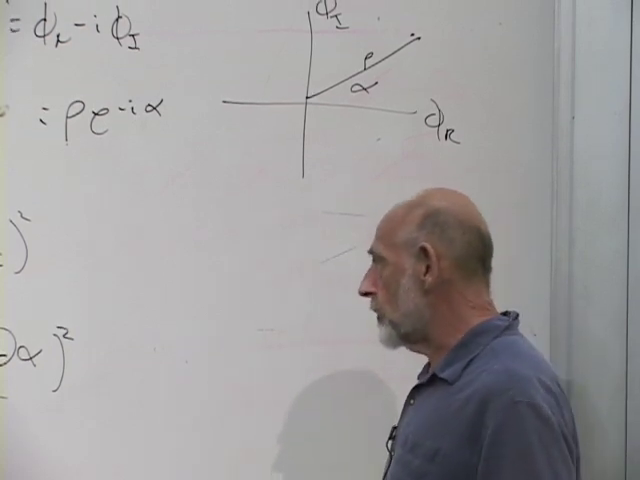
\includegraphics[width=0.72\textwidth]{lecture_08_figure_02.png}
\caption{El escalar complejo representado en su plano interno \((\phi_R,\phi_I)\). El radio es \(\rho\) y \(\alpha\) es la fase interna.}
\lectureframe{00:24:41}
\label{fig:l08-internal-plane}
\end{figure}

El término cinético del escalar se convierte en
\begin{align}
  \partial_\mu\phi^*\,\partial^\mu\phi
  &=
  \partial_\mu\phi_R\,\partial^\mu\phi_R
  +\partial_\mu\phi_I\,\partial^\mu\phi_I
  \notag\\
  &=
  \partial_\mu\rho\,\partial^\mu\rho
  +\rho^2\partial_\mu\alpha\,\partial^\mu\alpha.
  \label{eq:l08-polar-kinetic}
\end{align}
Un potencial invariante bajo \(U(1)\) global depende de \(\phi^*\phi=\rho^2\), no de \(\alpha\). Por ejemplo,
\begin{equation}
  V(\phi)
  =\lambda\left(\phi^*\phi-\frac{f^2}{2}\right)^2,
  \qquad \lambda>0.
  \label{eq:l08-mexican-hat}
\end{equation}
Sus mínimos forman un círculo. La ley es invariante bajo una rotación común de fase, pero elegir una fase de equilibrio selecciona un punto del círculo.

\begin{figure}[htbp]
\centering
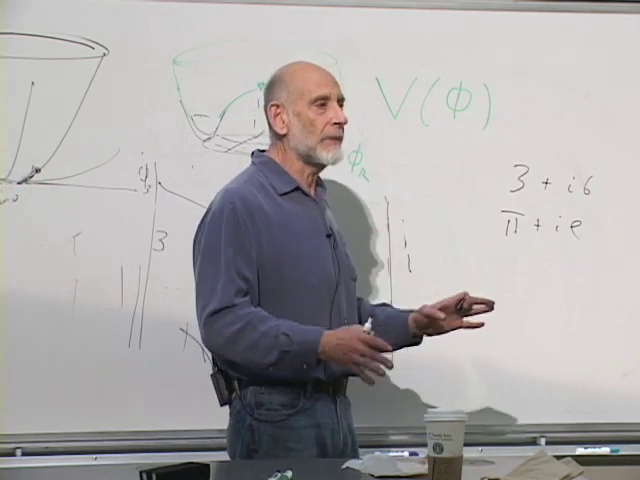
\includegraphics[width=0.78\textwidth]{lecture_08_figure_03.png}
\caption{Esquema del potencial radial dibujado en la pizarra. El potencial es simétrico bajo rotaciones del valor interno del campo, aunque el propio campo no tenga por qué estar en el origen.}
\lectureframe{00:34:22}
\label{fig:l08-radial-potential-board}
\end{figure}

\begin{figure}[htbp]
\centering
\begin{tikzpicture}[x=0.94cm,y=0.94cm]
  \draw[->] (-4.2,0) -- (4.4,0) node[right] {\(\phi_R\)};
  \draw[->] (0,-3.7) -- (0,3.9) node[above] {\(\phi_I\)};
  \draw[very thick,blue!65!black] (0,0) circle (2.45);
  \draw[->,very thick,orange!75!black] (0,0) -- (2.2,1.08);
  \draw[->,very thick,teal!70!black]
    (2.2,1.08) arc[start angle=26,end angle=67,radius=2.45];
  \node[orange!75!black,below right] at (1.15,0.52)
    {radial \(h\): massive};
  \node[teal!70!black,above right] at (1.78,1.76)
    {angular \(\pi\): massless};
  \fill (2.2,1.08) circle (2pt);
  \node[below] at (0,-2.65) {degenerate vacuum circle};
\end{tikzpicture}
\caption{La teoría global rota tiene curvatura normal al círculo de vacíos, pero no a lo largo de este. El modo radial de Higgs es masivo; el modo angular de Goldstone no tiene masa.}
\label{fig:l08-radial-angular}
\end{figure}

Definamos
\begin{equation}
  \phi(x)=\frac{f+h(x)}{\sqrt2}
           e^{i\pi(x)/f}.
  \label{eq:l08-canonical-polar}
\end{equation}
Cerca del vacío seleccionado, \(h\) mide el desplazamiento radial y \(\pi\) mide el desplazamiento tangencial, ambos con dimensiones canónicas. Al sustituir en la ec.~\eqref{eq:l08-polar-kinetic} se obtiene
\begin{equation}
  \partial_\mu\phi^*\,\partial^\mu\phi
  =
  \frac12(\partial_\mu h)^2
  +\frac12\left(1+\frac{h}{f}\right)^2
            (\partial_\mu\pi)^2.
  \label{eq:l08-global-expanded}
\end{equation}
El potencial de la ec.~\eqref{eq:l08-mexican-hat} aporta
\begin{equation}
  m_h^2=2\lambda f^2,
  \qquad
  m_\pi^2=0.
  \label{eq:l08-global-masses}
\end{equation}
A energías muy inferiores a \(m_h\), el movimiento radial resulta costoso, así que podemos fijar temporalmente \(h=0\). El lagrangiano restante contiene solo \(\frac12(\partial\pi)^2\), sin término \(\pi^2\). Este es el bosón de Goldstone.\editorialnote{En dos momentos, la explicación oral invierte los nombres y dice que, al engullir el Goldstone, el bosón de Higgs adquiere masa. El cálculo de la pizarra y el resto de la clase establecen el resultado pretendido: la curvatura radial ya confiere masa al modo de Higgs, mientras que el bosón gauge adquiere el modo de Goldstone y se vuelve masivo.}

\begin{classroomqa}
\audiencequestion{¿Es esta la única ruptura espontánea de simetría en el modelo estándar?\lecturetimestamp{00:16:39}}
\lecturerresponse{La fase de Higgs electrodébil es el mecanismo de ruptura de simetría establecido que nos interesa aquí. La simetría real es \(SU(2)_L\times U(1)_Y\), no este único \(U(1)\), y la QCD tiene otras estructuras del vacío, como la ruptura de la simetría quiral. El ejemplo abeliano es un modelo deliberadamente reducido del mecanismo de adquisición de masa de los bosones gauge.}
\end{classroomqa}

\begin{classroomqa}
\audiencequestion{¿El Higgs da masa a todas las partículas, incluida él mismo?\lecturetimestamp{00:17:11}}
\lecturerresponse{Hay que distinguir entre un sí y un no. La simetría electrodébil prohíbe masas desnudas para \(W\), \(Z\) y los fermiones del modelo estándar; sus masas aparecen cuando el campo de Higgs adquiere una magnitud de equilibrio distinta de cero. La masa radial del Higgs proviene de la curvatura de su propio potencial. Otras partículas hipotéticas pueden tener masas permitidas por la simetría y ajenas a este mecanismo.}
\end{classroomqa}

La clase relaciona esas masas permitidas por la simetría con partículas potencialmente muy pesadas y difíciles de observar, y menciona la materia oscura como posible ejemplo. Se trata de una motivación, no de una predicción de masa.
\editorialnote{La escala de masa de la materia oscura sigue siendo desconocida. La sugerencia de la clase de que podría tratarse de una partícula con una masa de alrededor de mil veces la masa del protón es una especulación histórica, no una propiedad de la materia oscura establecida experimentalmente.}

\begin{classroomqa}
\audiencequestion{¿\(\rho\) es un radio físico o el valor del campo? ¿Qué es exactamente lo que tiene simetría radial?\lecturetimestamp{00:33:08}}
\lecturerresponse{En cada punto del espacio-tiempo, el valor del campo es un punto de un plano complejo auxiliar, y \(\rho=|\phi|\) es la distancia de ese punto al origen. El \emph{potencial} tiene simetría radial en este plano interno: todos los puntos con el mismo \(\rho\) tienen la misma energía potencial. Este radio no es una distancia en el espacio ordinario.}
\end{classroomqa}

\begin{classroomqa}
\audiencequestion{¿Podría una perturbación radial lo bastante violenta llevar el campo por encima del máximo central hasta el otro lado del potencial?
\lecturetimestamp{00:36:00}}
\lecturerresponse{En principio, una configuración local con suficiente energía puede superar la barrera. Desplazar por encima de ella un campo macroscópico homogéneo requeriría una energía enorme, y una perturbación violenta genérica disiparía energía en muchos modos del campo en lugar de llegar coherentemente al punto opuesto. La aproximación de baja energía fija \(\rho\) precisamente porque en ese régimen no son accesibles excursiones radiales de ese tipo.}
\end{classroomqa}

\section{Por qué el plano complejo no es el espacio-tiempo}

La distinción entre coordenadas físicas e internas merece que nos detengamos en ella como en la clase. Un campo se llama escalar porque es invariante bajo rotaciones de los ejes de coordenadas físicas. Dos campos escalares reales \(\phi_R(x)\) y \(\phi_I(x)\) siguen siendo dos escalares bajo esas rotaciones. Podemos agruparlos en un solo número complejo, pero esta notación no los convierte en componentes de un vector espacial.

Una transformación global \(U(1)\) rota los \emph{valores} del campo:
\begin{equation}
\begin{aligned}
  \phi(x)&\longmapsto e^{i\theta}\phi(x),
  \\
  \rho(x)&\longmapsto\rho(x),
  \\
  \alpha(x)&\longmapsto\alpha(x)+\theta.
\end{aligned}
  \label{eq:l08-global-shift}
\end{equation}
Se usa la misma constante \(\theta\) en todos los puntos del espacio-tiempo. En consecuencia, \(\partial_\mu\alpha\) no cambia. Esta es una simetría tanto del potencial como del término cinético ordinario. Si se permite que \(\theta\) dependa de \(x\), la derivada detecta esa variación y el argumento cambia.

\section{Hacer local la rotación de fase}

\subsection{La derivada ordinaria deja de funcionar}

Sea
\begin{equation}
  \phi'(x)=e^{i\theta(x)}\phi(x).
  \label{eq:l08-local-phase}
\end{equation}
Entonces
\begin{equation}
  \partial_\mu\phi'
  =e^{i\theta}
    \left(\partial_\mu\phi+i\,\partial_\mu\theta\,\phi\right).
  \label{eq:l08-ordinary-derivative-fails}
\end{equation}
El término adicional proporcional a \(\partial_\mu\theta\) impide que \(\partial_\mu\phi\) se transforme como \(\phi\). Por tanto, \(\partial_\mu\phi^*\partial^\mu\phi\) no es invariante bajo rotaciones de fase locales arbitrarias.

\begin{figure}[htbp]
\centering
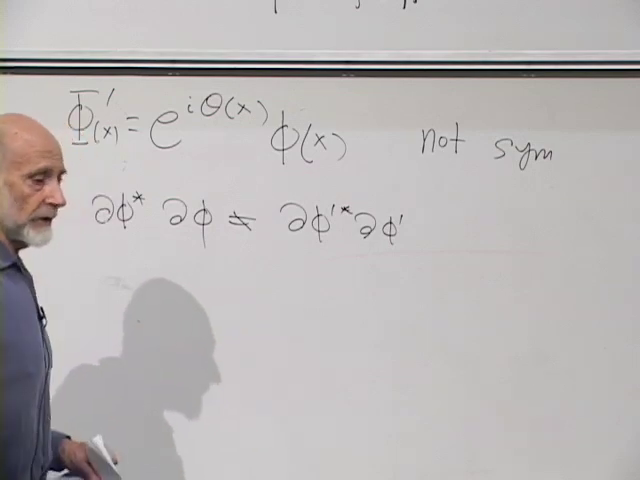
\includegraphics[width=0.78\textwidth]{lecture_08_figure_04.png}
\caption{La pizarra recoge la transformación local de fase y muestra que el término con la derivada ordinaria no conserva la invariancia.}
\lectureframe{00:46:49}
\label{fig:l08-local-not-symmetry}
\end{figure}

Introduzcamos un potencial vector y fijemos una convención para usarla coherentemente:
\begin{equation}
  D_\mu=\partial_\mu+i g A_\mu,
  \qquad
  A_\mu'=A_\mu-\frac1g\partial_\mu\theta.
  \label{eq:l08-covariant-convention}
\end{equation}
Ahora,
\begin{align}
  D_\mu'\phi'
  &=
  \left(\partial_\mu+i g A_\mu'\right)
  e^{i\theta}\phi
  \notag\\
  &=
  e^{i\theta}
  \left[
    \partial_\mu\phi+i(\partial_\mu\theta)\phi
    +i g A_\mu\phi-i(\partial_\mu\theta)\phi
  \right]
  \notag\\
  &=e^{i\theta}D_\mu\phi.
  \label{eq:l08-covariant-transform}
\end{align}
Los términos no deseados se cancelan. La derivada conjugada es
\begin{equation}
  (D_\mu\phi)^*
  =(\partial_\mu-i g A_\mu)\phi^*,
\end{equation}
y su fase opuesta se cancela en el producto
\begin{equation}
  (D_\mu\phi)^*D^\mu\phi.
\end{equation}

\begin{classroomqa}
\audiencequestion{¿En la clase anterior se escribió con el signo opuesto la transformación del campo gauge?\lecturetimestamp{00:48:04}}
\lecturerresponse{Invertir simultáneamente el signo en \(D_\mu\) y en la ley de transformación es solo una convención. Con \(D_\mu=\partial_\mu+i gA_\mu\) y \(\phi'=e^{i\theta}\phi\), la coherencia exige \(A_\mu'=A_\mu-g^{-1}\partial_\mu\theta\). La convención alternativa funciona igual de bien si se cambian todos los signos a la vez.}
\end{classroomqa}

\begin{classroomqa}
\audiencequestion{¿El uso de una forma mayúscula o minúscula de \(\phi\) en la pizarra indica un campo distinto?\lecturetimestamp{00:55:02}}
\lecturerresponse{No se pretende indicar ninguna diferencia. La variación en la forma de la letra se debe a la caligrafía; no indica una operación adicional ni un segundo escalar. Las distinciones con significado son la prima, el asterisco de conjugación compleja y el índice espacio-temporal.}
\end{classroomqa}

\begin{classroomqa}
\audiencequestion{¿Es la conjugación compleja la misma operación que subir o bajar el índice de Lorentz en el término cinético?
\lecturetimestamp{00:56:50}}
\lecturerresponse{No. El asterisco conjuga el campo complejo interno. Los índices de Lorentz se suben con la métrica del espacio-tiempo:
\(D^\mu=g^{\mu\nu}D_\nu\). Un escalar de Lorentz requiere la contracción \((D_\mu\phi)^*D^\mu\phi\); ambas operaciones aparecen y cumplen funciones distintas.}
\end{classroomqa}

\subsection{El campo gauge tiene su propia dinámica}

El tensor de campo
\begin{equation}
  F_{\mu\nu}=\partial_\mu A_\nu-\partial_\nu A_\mu
  \label{eq:l08-field-strength}
\end{equation}
es invariante gauge porque se cancelan las dos derivadas segundas mixtas de \(\theta\). Sus componentes temporales--espaciales contienen el campo eléctrico, y sus componentes espaciales--espaciales contienen el campo magnético. Por tanto, la electrodinámica escalar queda descrita por
\begin{equation}
  \mathcal L
  =(D_\mu\phi)^*D^\mu\phi
  -V(\phi^*\phi)
  -\frac14F_{\mu\nu}F^{\mu\nu}.
  \label{eq:l08-abelian-higgs}
\end{equation}
El campo cargado que aparece aquí es bosónico. No es el campo del electrón, que es un fermión. Un núcleo de helio cargado o un condensado de pares de Cooper ilustran cómo puede surgir un grado de libertad bosónico cargado.

Antes de la ruptura de simetría, el término gauge contiene derivadas de \(A_\mu\), pero ningún término de masa directo. Podríamos intentar añadir
\begin{equation}
  \frac12m_A^2A_\mu A^\mu,
\end{equation}
pero, bajo la ec.~\eqref{eq:l08-covariant-convention},
\begin{equation}
  A_\mu A^\mu
  \longmapsto
  \left(A_\mu-\frac1g\partial_\mu\theta\right)
  \left(A^\mu-\frac1g\partial^\mu\theta\right),
  \label{eq:l08-bare-mass-fails}
\end{equation}
que no es igual a \(A_\mu A^\mu\). La simetría local prohíbe una masa desnuda para el bosón gauge.

\begin{figure}[htbp]
\centering
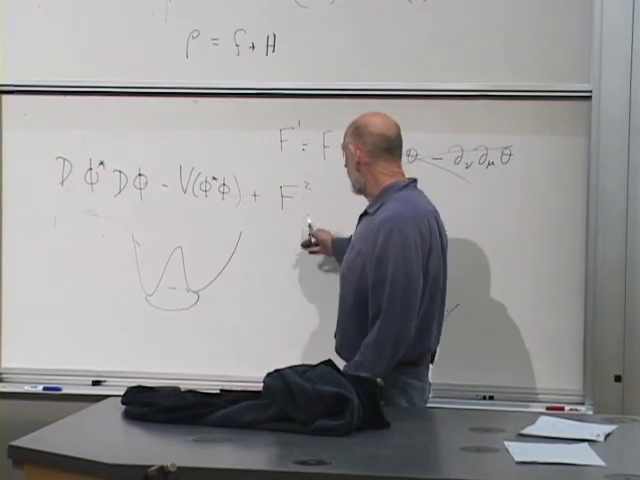
\includegraphics[width=0.76\textwidth]{lecture_08_figure_05.png}
\caption{La pizarra muestra el obstáculo: bajo una transformación gauge, \(A_\mu A^\mu\) se convierte en un cuadrado que contiene \(\partial_\mu\theta\), por lo que un término de masa desnudo para el vector no es invariante.}
\lectureframe{01:07:30}
\label{fig:l08-bare-mass-board}
\end{figure}

\section{El mecanismo de Higgs}

\subsection{La derivada covariante produce la masa}

Volvamos al potencial roto y usemos la parametrización con normalización canónica
\begin{equation}
  \phi(x)=\frac{f+h(x)}{\sqrt2}
  e^{i\pi(x)/f}.
\end{equation}
Su derivada covariante es
\begin{equation}
  D_\mu\phi
  =
  \frac{e^{i\pi/f}}{\sqrt2}
  \left[
    \partial_\mu h
    +i(f+h)
      \left(\frac{\partial_\mu\pi}{f}+gA_\mu\right)
  \right].
  \label{eq:l08-covariant-polar}
\end{equation}
Por consiguiente,
\begin{equation}
\begin{aligned}
  (D_\mu\phi)^*D^\mu\phi
  ={}&
  \frac12(\partial_\mu h)^2
  \\
  &+\frac12(f+h)^2
    \left(\frac{\partial_\mu\pi}{f}+gA_\mu\right)
  \\
  &\hspace{4.2em}\times
    \left(\frac{\partial^\mu\pi}{f}+gA^\mu\right).
\end{aligned}
  \label{eq:l08-higgs-kinetic}
\end{equation}

El término decisivo aparece antes de elegir ningún gauge:
\begin{equation}
  \frac12g^2f^2 A_\mu A^\mu.
  \label{eq:l08-vector-mass-term}
\end{equation}
Al compararlo con la forma de Proca \(\frac12m_A^2A_\mu A^\mu\), encontramos
\begin{equation}
  \boxed{m_A=g f}.
  \label{eq:l08-vector-mass}
\end{equation}
El mismo desarrollo también produce interacciones \(g^2fh A_\mu A^\mu\) y \(\frac12g^2h^2A_\mu A^\mu\). Por tanto, la masa del vector no es una violación arbitraria de la simetría gauge. Proviene de un término cinético escalar invariante gauge evaluado en una fase con magnitud de equilibrio \(f\) distinta de cero.

\begin{figure}[htbp]
\centering
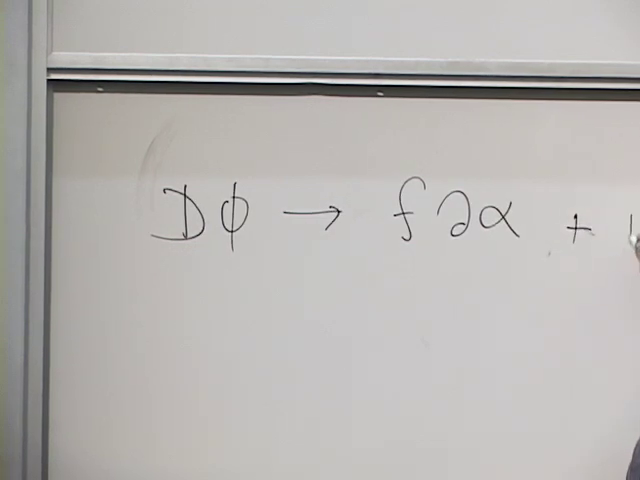
\includegraphics[width=0.78\textwidth]{lecture_08_figure_06.png}
\caption{La pizarra separa la contribución \(f^2A^2\) contenida en \((D\phi)^*(D\phi)\). Los factores numéricos dependen de cómo se normalicen el campo escalar y el acoplamiento gauge; con las ecs.~\eqref{eq:l08-canonical-polar} y \eqref{eq:l08-covariant-convention}, el resultado es \(m_A=gf\).}
\lectureframe{01:10:10}
\label{fig:l08-generated-mass-board}
\end{figure}

La clase incorpora \(g\) y varios factores de \(\sqrt2\) a la notación de la pizarra; por eso, al identificar la masa, alterna brevemente entre \(f\), \(2f\) y \(\sqrt2f\). Esos factores no tienen un significado invariante mientras no se especifiquen las normalizaciones cinética y del potencial. El resultado robusto es \(m_A\propto gf\); la ec.~\eqref{eq:l08-vector-mass} da el factor correspondiente a la convención usada aquí.

\subsection{La fase queda absorbida}

Bajo una transformación gauge, la variable de fase cambia según
\begin{equation}
  \pi'(x)=\pi(x)+f\,\theta(x).
\end{equation}
Elijamos
\begin{equation}
  \theta(x)=-\frac{\pi(x)}{f}.
  \label{eq:l08-unitary-gauge-choice}
\end{equation}
Entonces \(\pi'=0\). Este es el gauge unitario, en el que \begin{equation}
  \phi'(x)=\frac{f+h(x)}{\sqrt2}
\end{equation} es real, y la ec.~\eqref{eq:l08-higgs-kinetic} se reduce a
\begin{equation}
  (D_\mu\phi')^*D^\mu\phi'
  =
  \frac12(\partial_\mu h)^2
  +\frac12g^2(f+h)^2A_\mu'A^{\prime\mu}.
  \label{eq:l08-unitary-gauge-lagrangian}
\end{equation}
El campo de Goldstone angular ha desaparecido de la lista de variables independientes, mientras que la masa del vector permanece.

La clase muestra primero este resultado en el límite de baja energía \(\rho=f\), donde
\begin{align}
  \phi&=f e^{i\alpha},
  \notag\\
  D_\mu\phi
  &=if e^{i\alpha}
    \left(\partial_\mu\alpha+gA_\mu\right),
  \notag\\
  (D_\mu\phi)^*
  &=-if e^{-i\alpha}
    \left(\partial_\mu\alpha+gA_\mu\right).
  \label{eq:l08-frozen-radius}
\end{align}
Su producto es
\begin{equation}
  f^2
  \left(\partial_\mu\alpha+gA_\mu\right)
  \left(\partial^\mu\alpha+gA^\mu\right).
\end{equation}
La elección \(\theta=-\alpha\) deja \(g^2f^2A_\mu'A^{\prime\mu}\).

\begin{figure}[htbp]
\centering
\includegraphics[width=0.82\textwidth]{lecture_08_figure_07.png}
\caption{La pizarra muestra el desarrollo completo con radio fijo: las derivadas covariantes contienen conjuntamente la derivada de la fase y el potencial vector. A continuación, la clase elige \(\theta=-\alpha\), elimina la fase y deja el término de masa del vector.}
\lectureframe{01:16:20}
\label{fig:l08-frozen-radius-board}
\end{figure}

\begin{classroomqa}
\audiencequestion{¿Se puede reescribir todo el lagrangiano en variables que hagan explícita la desaparición del modo angular?
\lecturetimestamp{01:13:49}}
\lecturerresponse{Sí. En coordenadas polares, la fase solo aparece en la combinación invariante gauge \(\partial_\mu\alpha+gA_\mu\). Una transformación gauge con \(\theta=-\alpha\) fija la fase en cero en todos los puntos donde este gauge esté bien definido. El término cinético escalar se convierte entonces en un término de masa para el vector, mientras que el término invariante gauge del tensor de campo no cambia.}
\end{classroomqa}

\begin{classroomqa}
\audiencequestion{¿Son indistinguibles las oscilaciones de \(\alpha\) y las oscilaciones gauge?\lecturetimestamp{01:18:02}}
\lecturerresponse{En la teoría gauge, un cambio puro de \(\alpha\) compensado por el cambio correspondiente de \(A_\mu\) es una redescripción gauge, no una onda física distinta. La cantidad invariante es \(\partial_\mu\alpha+gA_\mu\). El modo físico que estaba representado por el campo global de Goldstone reaparece como la polarización longitudinal del vector masivo.}
\end{classroomqa}

Es habitual decir que una simetría gauge local se rompe espontáneamente. Esta expresión es útil en términos operativos: después de elegir un gauge, el campo escalar tiene un valor de vacío distinto de cero y el espectro contiene un vector masivo. Sin embargo, en sentido estricto, las transformaciones gauge relacionan descripciones redundantes, no estados físicos distintos.
\editorialnote{La redundancia gauge local no se rompe en el mismo sentido invariante gauge que una simetría global. La formulación precisa es que la teoría está en una fase de Higgs. La teoría de perturbaciones fijada en un gauge describe esa fase mediante un valor esperado escalar distinto de cero y el espectro resultante de vectores masivos.}

\section{Adónde fue el grado de libertad de Goldstone}

Nada físico puede desaparecer simplemente porque hayamos cambiado de variables. Contemos los grados de libertad antes y después de entrar en la fase de Higgs.

Antes:
\begin{equation}
  \underbrace{2}_{\text{massless vector}}
  +
  \underbrace{2}_{\text{complex scalar}}
  =4.
\end{equation}
Un vector sin masa tiene dos polarizaciones transversales. El escalar complejo tiene dos componentes reales: una radial y otra angular.

Después:
\begin{equation}
  \underbrace{3}_{\text{massive vector}}
  +
  \underbrace{1}_{\text{radial Higgs}}
  =4.
  \label{eq:l08-degree-count}
\end{equation}
Un vector masivo puede ponerse en reposo. En su sistema de reposo no hay ninguna dirección espacial privilegiada, así que debe tener tres estados de polarización. Cuando se mueve, dos son transversales y uno es longitudinal. El modo de Goldstone se ha convertido en esa polarización longitudinal.

\begin{figure}[htbp]
\centering
\begin{adjustbox}{max width=\linewidth}
\begin{tikzpicture}[x=1cm,y=1cm]
  \node[draw,rounded corners,fill=blue!7,minimum width=4.3cm,
        minimum height=2.1cm,align=center] (before) at (0,0)
    {massless \(A_\mu\): \(2\) transverse\\
     \(+\)\\
     complex \(\phi\): \(h+\pi\)};
  \node[draw,rounded corners,fill=orange!10,minimum width=4.3cm,
        minimum height=2.1cm,align=center] (after) at (7,0)
    {massive \(A_\mu\): \(2\) transverse\\
     \(+\;1\) longitudinal\\
     \(+\) radial \(h\)};
  \draw[->,very thick] (before) -- node[above]{Higgs phase} (after);
  \draw[->,teal!70!black,thick]
    (-0.15,-0.65) to[bend right=28]
    node[below,align=center]{Goldstone \(\pi\) supplies\\longitudinal mode}
    (6.8,-0.65);
\end{tikzpicture}
\end{adjustbox}
\caption{El mecanismo de Higgs reorganiza los grados de libertad físicos, no los destruye.}
\label{fig:l08-degree-rearrangement}
\end{figure}

\begin{classroomqa}
\audiencequestion{¿Cómo puede desaparecer el grado de libertad angular sin violar el recuento de grados de libertad?\lecturetimestamp{01:19:13}}
\lecturerresponse{No desaparece físicamente. Un vector sin masa tiene dos helicidades porque no se puede poner en reposo. Un vector masivo tiene tres polarizaciones, incluida una longitudinal. El modo de Goldstone se convierte en esa tercera polarización, de modo que el número total de grados de libertad no cambia.}
\end{classroomqa}

La clase propone una prueba cinemática útil. Imaginemos una partícula vectorial masiva, reduzcamos su velocidad hasta detenerla y acelerémosla en una dirección nueva. Una polarización que era transversal respecto del movimiento inicial puede volverse longitudinal respecto del nuevo movimiento. Del mismo modo, si una partícula masiva con polarización circular pasa por el reposo y se envía en la dirección opuesta, se invierte su etiqueta de helicidad. No se puede hacer este experimento con una partícula estrictamente sin masa, porque ningún sistema inercial puede ponerla en reposo. Por tanto, sus dos helicidades constituyen un espectro físico coherente.

\section{La analogía superconductora}

En un superconductor convencional, los electrones forman pares de Cooper. Cada par es un bosón con carga eléctrica \(2e\), y el condensado se describe mediante un parámetro de orden complejo cargado. Cuando su magnitud es distinta de cero, la combinación de su fase y el potencial vector electromagnético produce el mecanismo de Anderson--Higgs. Los campos magnéticos estáticos decaen a lo largo de la profundidad de penetración de London, en vez de extenderse libremente por el interior del material. En este sentido preciso y dependiente del medio, el fotón se comporta como si hubiera adquirido masa.

Este ejemplo también aclara la distinción inicial. El campo electromagnético no se convierte de manera permanente en otra partícula elemental. La ley de propagación masiva corresponde al estado colectivo dentro del material; fuera de él, el fotón del vacío sigue sin tener masa.

\section{Qué se ha establecido}

Ahora podemos condensar el argumento sin perder su lógica:
\begin{enumerate}
  \item Una simetría continua global rota tiene una dirección angular plana y, por tanto, un modo de Goldstone sin masa.
  \item La invariancia local de fase requiere un potencial gauge y reemplaza \(\partial_\mu\) por \(D_\mu\).
  \item Una masa desnuda \(A_\mu A^\mu\) viola la ley de transformación local.
  \item Cuando el escalar cargado tiene una magnitud de equilibrio \(f\) distinta de cero, el término invariante gauge \(|D_\mu\phi|^2\) contiene \(\frac12g^2f^2A_\mu A^\mu\).
  \item El modo de fase puede eliminarse mediante una elección de gauge, y su grado de libertad físico se convierte en la polarización longitudinal del vector masivo.
  \item La excitación radial de Higgs permanece; su masa viene determinada por la curvatura del potencial escalar.
\end{enumerate}

La siguiente tarea es dar masa a los fermiones. Los electrones y los quarks no pueden emplear directamente el mecanismo vectorial; sus acoplamientos con el Higgs son interacciones de Yukawa. Cuando el escalar se estabiliza en \(f\), esas interacciones se convierten en términos de masa fermiónica.

La afirmación general de que las partículas conocidas serían sin masa sin la ruptura de simetría electrodébil requiere una última precisión. Las masas de los quarks elementales y los leptones cargados, así como las de \(W\) y \(Z\), sí se anulan junto con el valor esperado del Higgs. Sin embargo, la mayor parte de la masa del protón y del neutrón surge dinámicamente del confinamiento de la QCD y de la energía del campo fuerte, y no de las masas de los quarks debidas al Higgs. Esta distinción no altera el mecanismo de Higgs derivado aquí; delimita con precisión su ámbito de aplicación.

\chapter{Masas de los fermiones: quiralidad, acoplamientos de Yukawa y neutrinos de Majorana}

\lectureoverview{Primero reconstruimos el mecanismo de Higgs de los bosones de gauge en una teoría de juguete \(U(1)\) y luego planteamos la pregunta análoga para los fermiones. Una masa de Dirac mezcla campos quirales izquierdos y derechos, pero la interacción débil les asigna cargas distintas y, por tanto, prohíbe una masa desnuda. Un acoplamiento de Yukawa al campo de Higgs respeta la simetría; cuando el campo de Higgs adquiere un valor en el vacío, esa misma interacción se convierte en una masa fermiónica y en un acoplamiento medible de Higgs--fermión. La última parte sigue esta lógica y la aplica a la masa de los neutrinos, a posibles partículas pesadas sin protección, a la cinemática de los rayos cósmicos, a la inercia relativista y a la gravedad.}

El propósito de este repaso inicial no es simplemente repetir la clase anterior. Necesitamos rescatar una idea y expresarla de modo que podamos aplicarla a los fermiones: una masa corresponde a una energía no nula para una excitación de momento nulo. En un campo, momento nulo significa longitud de onda infinita, o un desplazamiento igual en todas partes. Una teoría que solo contiene derivadas no puede detectar un desplazamiento uniforme. Un término sin derivadas sí puede hacerlo.

\section{El mecanismo de los bosones gauge, en pocas palabras}

\subsection{Energía de las derivadas y un vector sin masa}

El campo gauge del modelo es \(A_\mu\), cuya intensidad de campo es
\begin{equation}
  F_{\mu\nu}
  =\partial_\mu A_\nu-\partial_\nu A_\mu .
  \label{eq:l09-field-strength}
\end{equation}
En la pizarra, el término cinético gauge se escribe de forma esquemática como \(F^2\). Con una normalización estándar, es
\begin{equation}
  \mathcal L_{\mathrm{gauge}}
  =-\frac14 F_{\mu\nu}F^{\mu\nu}.
  \label{eq:l09-gauge-kinetic}
\end{equation}

\begin{figure}[htbp]
\centering
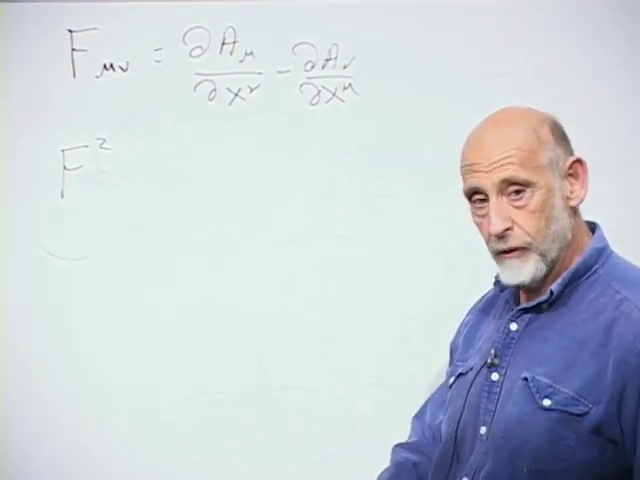
\includegraphics[width=0.72\textwidth]{lecture_09_figure_02.png}
\caption{La definición de la intensidad de campo y la notación abreviada \(F^2\) de la pizarra para la energía de las derivadas del campo gauge.}
\lectureframe{00:02:39}
\label{fig:l09-field-strength-board}
\end{figure}

Cada aparición de \(A_\mu\) en \eqref{eq:l09-gauge-kinetic} está sometida a una derivada. En consecuencia,
\begin{equation}
  A_\mu(x)\longmapsto A_\mu(x)+c_\mu,
  \qquad \partial_\nu c_\mu=0,
\end{equation}
no altera \(F_{\mu\nu}\). Por tanto, un potencial vector homogéneo no cuesta energía de intensidad de campo. En el lenguaje de la clase, el modo de momento nulo no tiene brecha y el bosón gauge no tiene masa.

Este campo \(U(1)\) es un sustituto deliberadamente sencillo. El objetivo físico son los bosones \(W^\pm\) y \(Z\), no el fotón electromagnético. La simetría electromagnética no rota mantiene al fotón sin masa; la simetría electrodébil rota da masa a los bosones gauge débiles.

\subsection{Fijar el módulo del campo de Higgs}

Introduzcamos un escalar complejo cargado y escribámoslo en forma polar:
\begin{equation}
  \phi(x)=\rho(x)e^{i\alpha(x)}.
\end{equation}
El potencial de sombrero mexicano alcanza su mínimo en una circunferencia de radio distinto de cero. Llamemos \(f\) a ese radio; la dirección radial es relativamente rígida. En esta primera aproximación, la fijamos y conservamos solo la fase:
\begin{equation}
  \phi(x)\simeq f e^{i\alpha(x)}.
  \label{eq:l09-frozen-higgs}
\end{equation}

\begin{figure}[htbp]
\centering
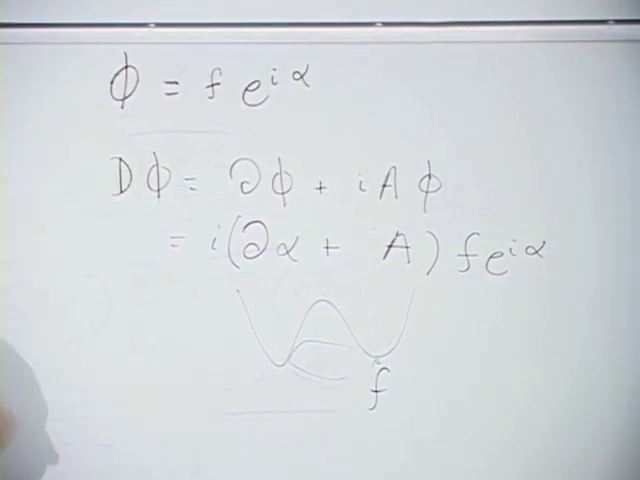
\includegraphics[width=0.72\textwidth]{lecture_09_figure_03.png}
\caption{El módulo fijado del campo de Higgs, su derivada covariante y el pequeño esquema del potencial con simetría rota utilizado en el repaso.}
\lectureframe{00:06:42}
\label{fig:l09-frozen-board}
\end{figure}

Elijamos la convención
\begin{equation}
\begin{aligned}
  D_\mu&=\partial_\mu+igA_\mu,
  \\
  \phi&\longmapsto e^{i\theta}\phi,
  \\
  A_\mu&\longmapsto A_\mu-\frac1g\partial_\mu\theta .
\end{aligned}
  \label{eq:l09-gauge-convention}
\end{equation}
En la clase se omite \(g\); dejarlo explícito permite ver con claridad las dimensiones y la masa que aparece al final. Al actuar sobre el campo con módulo fijado, se obtiene
\begin{align}
  D_\mu\phi
  &=(\partial_\mu+igA_\mu)f e^{i\alpha}
  \notag\\
  &=i\bigl(\partial_\mu\alpha+gA_\mu\bigr)
    f e^{i\alpha}.
  \label{eq:l09-covariant-frozen}
\end{align}
La multiplicación por el conjugado complejo elimina la fase y convierte también \(i\) por \(-i\) en \(+1\):
\begin{equation}
  |D_\mu\phi|^2
  =f^2
   \bigl(\partial_\mu\alpha+gA_\mu\bigr)
   \bigl(\partial^\mu\alpha+gA^\mu\bigr).
  \label{eq:l09-frozen-square}
\end{equation}

\begin{classroomqa}
\audiencequestion{¿Debe llevar un signo menos el cuadrado de la derivada covariante porque la derivada produce un factor de \(i\)?
\lecturetimestamp{00:07:39}}
\lecturerresponse{No. El término cinético es el producto por el conjugado complejo. Un factor aporta \(i\) y el otro \(-i\), de modo que \(i(-i)=1\). La convención de signo para \(D_\mu\) puede invertirse de manera consistente, pero el módulo al cuadrado es positivo en la expresión correspondiente para la energía.}
\end{classroomqa}

La combinación que aparece en \eqref{eq:l09-frozen-square} es por sí misma un campo gauge desplazado. Elijamos \(\theta=-\alpha\), de modo que desaparezca la fase escalar, y definamos
\begin{equation}
  A'_\mu=A_\mu+\frac1g\partial_\mu\alpha .
  \label{eq:l09-unitary-gauge-field}
\end{equation}
Entonces
\begin{equation}
  |D_\mu\phi|^2=g^2f^2 A'_\mu A'^\mu .
  \label{eq:l09-vector-mass-term}
\end{equation}
El nuevo término no contiene derivadas de \(A'_\mu\). Ahora un campo homogéneo almacena energía, así que el modo vectorial de momento nulo tiene una brecha.

\begin{figure}[htbp]
\centering
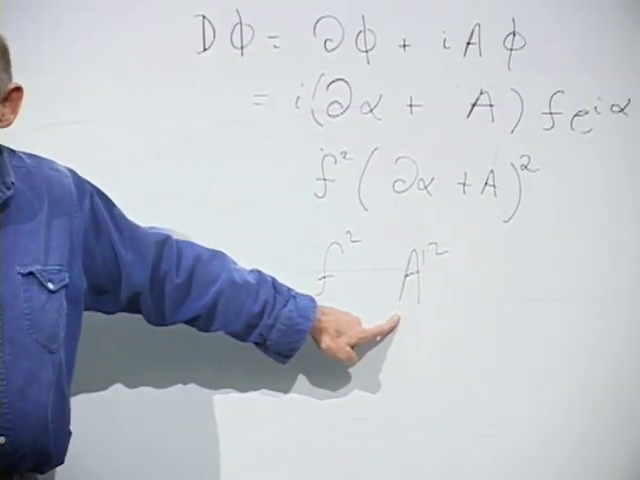
\includegraphics[width=0.72\textwidth]{lecture_09_figure_04.png}
\caption{La pizarra aísla el término \(f^2A^2\) que indica la aparición de una masa para el bosón gauge después de absorber la fase.}
\lectureframe{00:10:31}
\label{fig:l09-vector-mass-board}
\end{figure}

Con la normalización escalar canónica se escribe
\(\phi=(f+h)e^{i\pi/f}/\sqrt2\). Al comparar el término vectorial resultante con
\(\tfrac12m_A^2A_\mu A^\mu\), se obtiene
\begin{equation}
  m_A=gf
  \label{eq:l09-abelian-vector-mass}
\end{equation}
en este modelo abeliano. La clase omite los factores de normalización y resume el resultado diciendo que la masa vectorial viene determinada por \(f\).

La fase no desaparece sin dejar rastro. Antes de introducir el campo gauge, era un bosón de Goldstone sin masa. Una vez introducido, aporta la polarización longitudinal que necesita una partícula vectorial masiva. La fluctuación radial, que por ahora habíamos fijado, permanece como excitación física del Higgs.

\subsection{Por qué un término sin derivadas significa masa}

\begin{classroomqa}
\audiencequestion{¿Por qué se considera que un término \(A'^2\) representa una masa y no simplemente otra interacción?\lecturetimestamp{00:13:10}}
\lecturerresponse{La masa es energía en reposo. Para un campo, una partícula en reposo es el cuanto de un modo de momento nulo y longitud de onda infinita. El término con derivadas no aporta energía a un desplazamiento estático y homogéneo, mientras que \(m_A^2A'^2\) sí lo hace. Esa energía no nula a momento nulo es la brecha de energía en reposo.}
\end{classroomqa}

La clase desarrolla esta idea mediante tres analogías mecánicas.

\begin{itemize}
  \item En un cristal, un desplazamiento que varía lentamente cuesta energía elástica porque los átomos vecinos se desplazan de manera distinta. Una traslación rígida desplaza todos los átomos juntos y no cuesta energía interna. Por eso el fonón acústico no tiene brecha.
  \item En un imán ideal con simetría rotacional, la dirección del espín que varía en el espacio cuesta energía de intercambio, pero girar todos los espines juntos no. La onda de espín asociada, de longitud de onda larga, no tiene brecha.
  \item En un plasma, desplazar el fluido de electrones respecto del fondo positivo produce una separación de cargas y un campo eléctrico restaurador, incluso para un desplazamiento relativo homogéneo. El plasmón resultante tiene una frecuencia distinta de cero cuando el número de onda es nulo.
\end{itemize}

El campo gauge que adquiere masa mediante el mecanismo de Higgs se comporta como el tercer ejemplo: el medio con simetría rota se resiste a lo que, de otro modo, sería un desplazamiento homogéneo sin coste.

\begin{classroomqa}
\audiencequestion{Antes de introducir el campo gauge, ¿la fase \(\alpha\) no oscilaba ya?
\lecturetimestamp{00:18:24}}
\lecturerresponse{Sí. Su energía era proporcional a \(f^2(\partial_\mu\alpha)^2\). Una fase que varía de un lugar a otro tiene energía de gradiente y puede propagarse, pero un cambio uniforme de fase no cuesta energía. Eso es precisamente el modo de Goldstone sin masa.}
\end{classroomqa}

\begin{classroomqa}
\audiencequestion{La derivada incluye una derivada temporal. ¿Mover realmente toda la red o cambiar todo el campo no conlleva energía cinética?
\lecturetimestamp{00:22:18}}
\lecturerresponse{Sí. La comparación es entre configuraciones estáticas o entre configuraciones preparadas con una lentitud arbitraria. Una red que se traslada con velocidad distinta de cero tiene energía cinética. La prueba de la masa pregunta si la configuración conserva energía cuando está en reposo y es uniforme en el espacio.}
\end{classroomqa}

\section{La pista experimental: la interacción débil distingue entre izquierda y derecha}

La clase pasa ahora al electrón, el muón y los quarks. Sus masas también proceden del campo de Higgs, pero el mecanismo tiene otro aspecto porque la masa de un fermión no es un término vectorial cuadrático. Es un acoplamiento entre dos campos quirales.

\subsection{Violación de la paridad en la desintegración beta}

Partamos del hecho empírico de que la interacción débil viola la paridad. La electrodinámica cuántica y la cromodinámica cuántica tratan igual un proceso y su imagen especular. La interacción débil no lo hace. En la desintegración beta del neutrón,
\begin{equation}
  n\longrightarrow p+e^-+\bar\nu_e,
  \label{eq:l09-beta-decay}
\end{equation}
los electrones de alta energía seleccionados por la interacción de corriente cargada tienen helicidad levógira: su espín apunta en sentido opuesto a su momento. Los antineutrinos correspondientes tienen la helicidad opuesta.

Para una partícula ultrarrelativista, definimos la helicidad como
\begin{equation}
  h=\frac{\bm S\cdot\bm p}{|\bm S|\,|\bm p|}.
\end{equation}
El espín paralelo al momento corresponde a \(h=+1\); el espín antiparalelo, a \(h=-1\). La interacción débil se acopla a un campo electrónico quiral izquierdo y a un campo neutrínico quiral izquierdo, pero no de la misma manera a un campo electrónico quiral derecho.\editorialnote{Al principio, la clase emplea «levógiro» y «dextrógiro» en el sentido de la helicidad, porque resulta intuitivo visualizarlo a altas energías. Sin embargo, las cargas gauge actúan sobre la quiralidad, la etiqueta de la representación de Lorentz seleccionada por \(P_L=(1-\gamma^5)/2\) y \(P_R=(1+\gamma^5)/2\). Para una partícula sin masa, la quiralidad y la helicidad coinciden; para una partícula masiva, no.}

Para mostrar el obstáculo sin toda la contabilidad de \(SU(2)_L\times U(1)_Y\), imaginemos un mundo ficticio \(U(1)\) en el que solo \(\psi_L\) lleva la carga pertinente:
\begin{equation}
  \psi_L\longmapsto e^{i\theta}\psi_L,
  \qquad
  \psi_R\longmapsto\psi_R .
  \label{eq:l09-chiral-toy-charge}
\end{equation}
Esto no es electromagnetismo: los electrones reales de quiralidad izquierda y derecha tienen la misma carga eléctrica. Es una caricatura de la interacción débil, en la que las dos quiralidades pertenecen a representaciones electrodébiles distintas.

\begin{classroomqa}
\audiencequestion{¿Se da también en los quarks la misma asimetría izquierda--derecha?
\lecturetimestamp{00:31:50}}
\lecturerresponse{Sí, con los multipletes débiles y las hipercargas correspondientes. Los quarks de quiralidad izquierda, tanto de tipo up como de tipo down, forman dobletes débiles, mientras que los campos de quiralidad derecha son singletes débiles. Por tanto, sus acoplamientos con el Higgs presentan el mismo problema estructural que los del electrón.}
\end{classroomqa}

\section{Una masa de Dirac mezcla los estados de quiralidad izquierda--y derecha}

\subsection{De la ecuación de cuatro componentes a dos ecuaciones de Weyl}

Una función de onda de Dirac tiene cuatro componentes. Dicho de manera aproximada, dos describen el espín y las otras dos distinguen las soluciones de energía positiva y negativa; estas últimas se reinterpretan como grados de libertad de las antipartículas. En forma hamiltoniana,
\begin{equation}
  i\frac{\partial\Psi}{\partial t}
  =\left(-i\bm\alpha\cdot\bm\nabla+m\beta\right)\Psi .
  \label{eq:l09-dirac-hamiltonian}
\end{equation}
Las matrices \(\alpha_i\) y \(\beta\) codifican la relación relativista entre energía, momento y masa.

\begin{figure}[htbp]
\centering
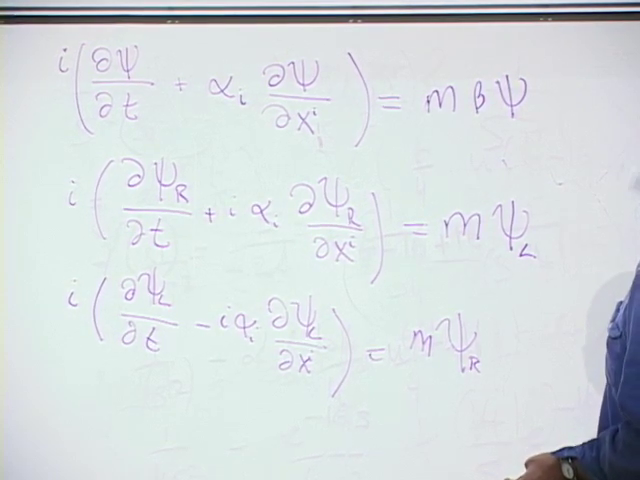
\includegraphics[width=0.74\textwidth]{lecture_09_figure_05.png}
\caption{La pizarra presenta primero la ecuación de Dirac y luego la descompone en ecuaciones acopladas de quiralidad izquierda y derecha.}
\lectureframe{00:40:30}
\label{fig:l09-dirac-board}
\end{figure}

La base quiral hace explícito el papel de \(m\). Con
\(\sigma^\mu=(1,\bm\sigma)\) y
\(\bar\sigma^\mu=(1,-\bm\sigma)\),
\begin{align}
  i\bar\sigma^\mu\partial_\mu\psi_L&=m\psi_R,
  \label{eq:l09-weyl-left}\\
  i\sigma^\mu\partial_\mu\psi_R&=m\psi_L.
  \label{eq:l09-weyl-right}
\end{align}
Cuando \(m=0\), las ecuaciones son independientes: un campo quiral izquierdo y uno quiral derecho pueden propagarse sin interactuar entre sí. Cuando \(m\neq0\), cada uno actúa como fuente del otro. Este es el sentido preciso en que una masa de Dirac mezcla las quiralidades izquierda y derecha.

Susskind describe esto diciendo que el fermión oscila entre los estados de quiralidad izquierda y derecha. Esa forma de expresarlo capta el acoplamiento, pero no debe llevarse hasta una imagen clásica literal de una partícula puntual que alterna de un estado a otro. La afirmación precisa es que la ecuación de campo es acoplada:
\eqref{eq:l09-weyl-left}--\eqref{eq:l09-weyl-right}.

\begin{classroomqa}
\audiencequestion{¿Son coherentes los factores de \(i\) y los signos de las dos ecuaciones de la pizarra?
\lecturetimestamp{00:41:10}}
\lecturerresponse{No, si se comparan línea por línea en la pizarra: durante la derivación rápida se sacó un factor \(i\) de forma inconsistente. Lo fiable es el patrón de acoplamiento. Las ecuaciones \eqref{eq:l09-weyl-left} y
\eqref{eq:l09-weyl-right} corresponden a una convención estándar coherente.}
\end{classroomqa}

\subsection{Por qué la simetría débil prohíbe una masa desnuda}

El término de masa de Dirac correspondiente en el lagrangiano es
\begin{equation}
  \mathcal L_m
  =-m\bar\psi\psi
  =-m\left(\bar\psi_L\psi_R+\bar\psi_R\psi_L\right).
  \label{eq:l09-bare-dirac-mass}
\end{equation}
Bajo la transformación de juguete \eqref{eq:l09-chiral-toy-charge},
\begin{equation}
  \bar\psi_L\psi_R\longmapsto
  e^{-i\theta}\bar\psi_L\psi_R,
  \qquad
  \bar\psi_R\psi_L\longmapsto
  e^{i\theta}\bar\psi_R\psi_L.
\end{equation}
Ninguno de los dos términos es invariante. Por tanto, el coeficiente de mezcla directa entre izquierda y derecha --\(m\) está prohibido antes de la ruptura de simetría.

El electromagnetismo por sí solo no plantearía este problema, porque \(\psi_L\) y \(\psi_R\) tienen la misma carga eléctrica. El obstáculo se debe a que sus números cuánticos débiles son distintos.

\subsection{Preguntas sobre helicidad que ponen de manifiesto la sutileza de la quiralidad}

Ahora la clase pone a prueba desde varios ángulos la imagen intuitiva de la quiralidad. Estas preguntas no son cuestiones secundarias: revelan con precisión dónde resulta útil la helicidad y dónde hay que recurrir a la quiralidad.

\begin{classroomqa}
\audiencequestion{¿Cómo sería el mundo si la interacción débil emitiera electrones de ambas helicidades en igual proporción?
\lecturetimestamp{00:42:12}}
\lecturerresponse{La asimetría de paridad inmediata desaparecería en ese proceso. Pero la teoría electrodébil real es quiral: solo los dobletes de quiralidad izquierda llevan la interacción débil de corriente cargada. La clase pospone una explicación más completa de por qué la naturaleza eligió esa estructura.}
\end{classroomqa}

\begin{classroomqa}
\audiencequestion{Supongamos que se prepara el espín de un electrón en dirección vertical y luego se acelera el electrón horizontalmente. ¿Es levógiro o dextrógiro?
\lecturetimestamp{00:42:44}}
\lecturerresponse{Un estado de espín transversal al momento es una superposición de las dos helicidades. La helicidad está bien definida solo cuando el espín es paralelo o antiparalelo al momento. Aun así, los proyectores quirales débiles del campo están bien definidos.}
\end{classroomqa}

Una partícula masiva puede frenarse hasta quedar en reposo y acelerarse en la dirección opuesta sin invertir su espín. Entonces cambia el signo de su helicidad. Una partícula sin masa no puede ser alcanzada ni llevada al reposo mediante una transformación de Lorentz, así que su helicidad es invariante bajo los boosts propios. Esto motiva la afirmación de la clase de que una especie con una sola helicidad física debe carecer de masa. La formulación más precisa en teoría de campos es que una masa de Dirac invariante de Lorentz requiere ambas quiralidades.

\begin{classroomqa}
\audiencequestion{Un fotón con polarización circular puede reflejarse en un espejo e invertir su dirección sin llegar nunca al reposo. ¿Contradice eso el argumento sobre la helicidad?
\lecturetimestamp{00:45:28}}
\lecturerresponse{No. El espejo es un sistema externo que puede intercambiar momento angular e invertir la dirección de propagación. Un proceso de reflexión no es un boost de Lorentz que alcanza al fotón. La existencia de un canal también depende de los estados de polarización permitidos y de las condiciones de contorno del material.}
\end{classroomqa}

\begin{classroomqa}
\audiencequestion{¿Un haz ordinario de electrones contiene una sola quiralidad o ambas?
\lecturetimestamp{00:46:10}}
\lecturerresponse{En general, ambas. Un estado de electrón masivo contiene componentes de las dos quiralidades, y un haz no polarizado contiene ambas helicidades. Las fuentes especializadas pueden producir un haz polarizado con una marcada asimetría de helicidad.}
\end{classroomqa}

\begin{classroomqa}
\audiencequestion{¿Se puede enfocar un haz sin depender del espín, o los campos magnéticos separan las dos polarizaciones?
\lecturetimestamp{00:46:29}}
\lecturerresponse{El enfoque ordinario de la posición puede ser en gran medida insensible al espín, pero los momentos magnéticos se acoplan a los gradientes del campo magnético. Por tanto, las fuentes selectivas en espín, los gradientes del tipo Stern--Gerlach y la dinámica del espín en los aceleradores permiten preparar o separar polarizaciones.}
\end{classroomqa}

\begin{classroomqa}
\audiencequestion{¿La diferencia entre izquierda y derecha en la interacción débil es simplemente accidental?
\lecturetimestamp{00:48:13}}
\lecturerresponse{En este curso, se considera un hecho experimental incorporado al modelo estándar. Su regularidad hace que no parezca un accidente fortuito, pero el propio modelo estándar no deriva el patrón completo de cargas quirales a partir de un principio más profundo.}
\end{classroomqa}

\section{La construcción de Yukawa}

\subsection{Asignar al Higgs la carga que falta}

La simetría prohíbe una masa numérica, pero permite una interacción con un campo que aporte la fase de transformación que falta. Introduzcamos un escalar complejo tal que
\begin{equation}
  \phi\longmapsto e^{i\theta}\phi,
  \qquad
  \phi^\dagger\longmapsto e^{-i\theta}\phi^\dagger.
  \label{eq:l09-scalar-charge}
\end{equation}
Entonces
\begin{equation}
  \mathcal L_Y
  =-y\,\bar\psi_L\phi\psi_R
   -y^*\,\bar\psi_R\phi^\dagger\psi_L
  \label{eq:l09-yukawa-lagrangian}
\end{equation}
es invariante gauge. En el primer término,
\(\bar\psi_L\) aporta \(e^{-i\theta}\) y \(\phi\) aporta
\(e^{i\theta}\); las fases se cancelan. El segundo término es su conjugado hermítico.

De forma equivalente, las ecuaciones quirales adquieren una mezcla dependiente del campo:
\begin{align}
  i\bar\sigma^\mu D_\mu\psi_L
    &=y\phi\psi_R,
  \label{eq:l09-yukawa-eom-left}\\
  i\sigma^\mu\partial_\mu\psi_R
    &=y^*\phi^\dagger\psi_L.
  \label{eq:l09-yukawa-eom-right}
\end{align}

\begin{figure}[htbp]
\centering
\includegraphics[width=0.76\textwidth]{lecture_09_figure_06.png}
\caption{La masa desnuda de los miembros derechos de las ecuaciones se ha sustituido por el campo escalar cargado. Los signos exactos de la pizarra son esquemáticos; la estructura invariante está dada en \eqref{eq:l09-yukawa-lagrangian}.}
\lectureframe{00:51:30}
\label{fig:l09-yukawa-board}
\end{figure}

Antes de la ruptura de simetría, esto es una interacción, no una masa. Un fermión de quiralidad derecha solo puede convertirse en uno de quiralidad izquierda mientras emite o absorbe el cuanto escalar necesario para equilibrar la carga. El coeficiente \(y\) es un acoplamiento de Yukawa, no la carga gauge \(g\).

\begin{classroomqa}
\audiencequestion{¿Es legítimo simplemente poner \(\phi\) y
\(\phi^\dagger\) en los miembros derechos de las dos ecuaciones?
\lecturetimestamp{00:51:55}}
\lecturerresponse{Es legítimo precisamente porque sus fases de transformación corrigen la discrepancia. La prueba decisiva no es la forma visual de la ecuación, sino la invariancia gauge de la interacción
\(\bar\psi_L\phi\psi_R+\mathrm{h.c.}\).}
\end{classroomqa}

\subsection{El vacío convierte la interacción en masa}

Ahora identifiquemos \(\phi\) con el campo de Higgs y dejemos que alcance un módulo no nulo en el vacío. Con la normalización simplificada de la clase,
\begin{equation}
  \phi\simeq f,
\end{equation}
por lo que \eqref{eq:l09-yukawa-lagrangian} contiene
\begin{equation}
  \mathcal L_Y
  \supset
  -yf\,\bar\psi_L\psi_R
  -y^*f\,\bar\psi_R\psi_L .
\end{equation}
Cuando corresponde, tras una redefinición de fase inocua, la masa del fermión es
\begin{equation}
  m_f=yf.
  \label{eq:l09-lecture-fermion-mass}
\end{equation}
Este es el análogo fermiónico del resultado vectorial \(m_A=gf\). El mismo valor de vacío del Higgs que aporta una polarización longitudinal a los bosones gauge débiles también aporta los números cuánticos débiles que faltan para unir los fermiones de quiralidad izquierda y derecha.

Con la convención de normalización canónica del modelo estándar,
\begin{equation}
  H(x)=\frac1{\sqrt2}
  \begin{pmatrix}
    0\\ v+h(x)
  \end{pmatrix},
  \qquad v\simeq246\ \mathrm{GeV},
  \label{eq:l09-sm-higgs-vacuum}
\end{equation}
y, por tanto,
\begin{equation}
  m_f=\frac{y_fv}{\sqrt2}.
  \label{eq:l09-sm-fermion-mass}
\end{equation}
La cantidad \(f\) de la clase y la cantidad convencional \(v/\sqrt2\) solo difieren por esta elección de normalización.

\begin{classroomqa}
\audiencequestion{Si solo el producto \(yf\) es una masa fermiónica, ¿cómo se pueden determinar por separado el acoplamiento \(y\) y la escala del vacío \(f\)?
\lecturetimestamp{00:55:36}}
\lecturerresponse{Una vez conocidos los acoplamientos gauge, las masas de los bosones gauge débiles determinan la escala del vacío. Después, la masa medida de un fermión determina su acoplamiento de Yukawa. En la teoría completa,
\(m_W=gv/2\), \(m_Z=v\sqrt{g^2+g'^2}/2\) y
\(y_f=\sqrt2m_f/v\).}
\end{classroomqa}

\begin{classroomqa}
\audiencequestion{¿La masa del bosón débil es de unos \(900\ \mathrm{GeV}\)?
\lecturetimestamp{00:57:43}}
\lecturerresponse{No; la clase corrige enseguida el lapsus y da un valor aproximado de \(90\ \mathrm{GeV}\). Más precisamente,
\(m_W\simeq80\ \mathrm{GeV}\) y \(m_Z\simeq91\ \mathrm{GeV}\), mientras que la escala subyacente del vacío es \(v\simeq246\ \mathrm{GeV}\).}
\end{classroomqa}

\subsection{Una sola escala del vacío, muchos acoplamientos de Yukawa}

Cada especie de fermión cargado tiene su propio acoplamiento de Yukawa:
\begin{equation}
  m_i=y_i f
  \qquad\text{(lecture normalization)}.
  \label{eq:l09-mass-family}
\end{equation}

\begin{figure}[htbp]
\centering
\includegraphics[width=0.76\textwidth]{lecture_09_figure_08.png}
\caption{La pizarra resume la dependencia de la especie como \(m_i=g_i f\); los \(g_i\) que aparecen allí son los acoplamientos de Yukawa que aquí llamamos \(y_i\).}
\lectureframe{01:16:30}
\label{fig:l09-mass-family-board}
\end{figure}

Para el electrón, la clase estima
\begin{equation}
  y_e\sim\frac{0.5\ \mathrm{MeV}}{10^2\ \mathrm{GeV}}
  \sim10^{-5}.
\end{equation}
Al usar el valor canónico \(v=246\ \mathrm{GeV}\) se obtiene el valor más preciso
\(y_e\simeq2.9\times10^{-6}\). En el extremo opuesto está el quark top:
\begin{equation}
  y_t=\frac{\sqrt2m_t}{v}\simeq1.
\end{equation}
Así pues, el mecanismo de Higgs explica cómo puede existir una masa invariante gauge, pero no explica la enorme jerarquía entre los \(y_i\). Las masas fermiónicas observadas simplemente traducen esa jerarquía a valores medidos.

\begin{classroomqa}
\audiencequestion{¿De verdad tiene el quark top un acoplamiento de Yukawa de orden unidad?
\lecturetimestamp{00:59:09}}
\lecturerresponse{Sí. Su masa es comparable a la escala electrodébil, así que su acoplamiento no es un número perturbativo diminuto como el del electrón. En la normalización moderna, \(y_t\) es cercano a la unidad.}
\end{classroomqa}

\subsection{Restituir la fluctuación física del Higgs}

Al fijar el escalar en su valor de vacío, ocultamos la excitación radial. Restituyámosla de manera esquemática:
\begin{equation}
  \phi(x)\simeq f+h(x).
\end{equation}
El factor de Yukawa pasa a ser
\begin{equation}
  y\phi\simeq yf+yh=m_f+yh.
  \label{eq:l09-mass-plus-higgs}
\end{equation}

\begin{figure}[htbp]
\centering
\includegraphics[width=0.76\textwidth]{lecture_09_figure_07.png}
\caption{La pizarra restituye la fluctuación del Higgs dentro del término de Yukawa: la parte constante produce la masa fermiónica y la parte fluctuante produce la emisión o absorción de un Higgs.}
\lectureframe{01:01:15}
\label{fig:l09-higgs-fluctuation-board}
\end{figure}

El primer término de \eqref{eq:l09-mass-plus-higgs} es la masa. El segundo es un vértice en el que un bosón de Higgs se acopla al fermión. En la notación canónica del modelo estándar,
\begin{equation}
  \mathcal L_Y
  \supset
  -m_f\bar\psi\psi
  -\frac{m_f}{v}h\bar\psi\psi.
  \label{eq:l09-higgs-fermion-vertex}
\end{equation}
El acoplamiento es proporcional a la masa del fermión. Por tanto, sujeto a las restricciones cinemáticas, los factores de color, el espacio de fases y los canales en competencia, el Higgs se acopla con más intensidad a los fermiones más pesados.

\begin{classroomqa}
\audiencequestion{¿Las constantes de acoplamiento son probabilidades en sí mismas?
\lecturetimestamp{01:03:35}}
\lecturerresponse{Intervienen en las amplitudes cuánticas. A menudo, una tasa sencilla es proporcional al módulo al cuadrado de una amplitud y, por tanto, al cuadrado de un acoplamiento; pero también influyen el espacio de fases, las sumas sobre espín, la interferencia, los lazos y los vértices múltiples. No se debe identificar directamente un acoplamiento con una probabilidad.}
\end{classroomqa}

\begin{classroomqa}
\audiencequestion{¿Este argumento supone que solo hay un campo de Higgs?
\lecturetimestamp{01:03:59}}
\lecturerresponse{Describe el modelo estándar mínimo, que tiene un doblete de Higgs complejo. Tres de sus cuatro componentes reales son absorbidos por \(W^\pm\) y \(Z\), y queda un escalar neutro físico. Las extensiones pueden incluir más dobletes u otros multipletes escalares. Los modelos supersimétricos suelen requerir dos dobletes de Higgs y, por tanto, contienen varios estados físicos del Higgs.}
\end{classroomqa}

Ahora podemos comparar esa expectativa histórica con los experimentos.
\editorialnote{Esta clase se grabó antes del descubrimiento del Higgs. ATLAS y CMS anunciaron en 2012 la observación de una partícula similar al Higgs, cuya masa se mide actualmente en torno a \(125\ \mathrm{GeV}\). Sus acoplamientos observados concuerdan en términos generales con el patrón del modelo estándar, en el que son proporcionales a la masa. La afirmación de que se desintegra preferentemente en partículas más pesadas siempre está sujeta a una salvedad cinemática: un par \(t\bar t\) en la capa de masa no cabe en un Higgs de \(125\ \mathrm{GeV}\).}

\section{Antipartículas, haces y significado de la quiralidad}

Antes de pasar a los neutrinos, la clase retoma varias preguntas prácticas sobre antipartículas y haces de acelerador.

\begin{classroomqa}
\audiencequestion{¿Qué quiralidad tiene la antipartícula de un electrón levógiro?
\lecturetimestamp{01:06:05}}
\lecturerresponse{En el límite ultrarrelativista, un campo electrónico de quiralidad izquierda aniquila electrones de helicidad levógira y crea positrones de helicidad dextrógira. Este es uno de los casos en que hay que distinguir cuidadosamente entre partícula y antipartícula, y entre quiralidad y helicidad.}
\end{classroomqa}

\begin{classroomqa}
\audiencequestion{¿Pueden colisionar un electrón y un positrón para producir un bosón \(Z\)?
\lecturetimestamp{01:07:13}}
\lecturerresponse{Sí, cuando su energía en el centro de masas coincide con la del canal permitido. Los colisionadores de electrones--positrones estudiaron con gran precisión la resonancia del \(Z\). En el proceso completo se conservan la carga y los demás números cuánticos.}
\end{classroomqa}

\begin{classroomqa}
\audiencequestion{¿Se producen todos los positrones mediante un único proceso débil especial?
\lecturetimestamp{01:07:37}}
\lecturerresponse{No. La producción de pares es un proceso electromagnético habitual. Por ejemplo, un electrón energético puede emitir un fotón virtual, que a su vez puede producir un par \(e^-e^+\) en el campo de otra partícula. La clase lo ilustra con un diagrama de Feynman.}
\end{classroomqa}

\begin{classroomqa}
\audiencequestion{¿Puede un acelerador lineal seleccionar la velocidad o la energía de sus electrones?
\lecturetimestamp{01:09:24}}
\lecturerresponse{Sí. Los campos de aceleración y la temporización permiten seleccionar un intervalo de energías. Cuando los electrones ya son ultrarrelativistas, su velocidad está extremadamente cerca de \(c\), así que la energía adicional del acelerador aumenta sobre todo el momento y la energía total, en lugar de aumentar la velocidad de forma apreciable.}
\end{classroomqa}

\begin{classroomqa}
\audiencequestion{¿Puede un acelerador preparar un haz con una sola polarización?
\lecturetimestamp{01:09:47}}
\lecturerresponse{Sí, aunque es técnicamente exigente. Se pueden preparar electrones con espín polarizado a baja energía mediante una fuente que dependa del espín y luego acelerarlos controlando la precesión del espín. Los colisionadores modernos cuantifican la polarización resultante del haz en vez de considerarla perfectamente pura.}
\end{classroomqa}

\section{Masa de los neutrinos y posibilidad de Majorana}

\subsection{Por qué la masa de los neutrinos obligó a ampliar el modelo}

El modelo estándar mínimo original incluía solo campos de neutrino con quiralidad izquierda y, por tanto, predecía neutrinos sin masa. Las oscilaciones de neutrinos muestran que al menos dos de sus autovalores de masa son distintos y que las masas de los neutrinos no son nulas, aunque sean diminutas comparadas con las de los fermiones cargados.

\begin{classroomqa}
\audiencequestion{¿Qué tan pequeñas son las masas de los neutrinos y dónde está su componente de quiralidad derecha?
\lecturetimestamp{01:10:38}}
\lecturerresponse{Las oscilaciones determinan diferencias de masas al cuadrado, no las masas absolutas. Las separaciones pertinentes corresponden a escalas de aproximadamente \(0.009\ \mathrm{eV}\) y \(0.05\ \mathrm{eV}\). Una descripción de Dirac añade neutrinos estériles de quiralidad derecha; una descripción de Majorana, en cambio, relaciona la quiralidad que falta con campos de neutrino conjugados de carga.}
\end{classroomqa}

Para describir un neutrino de Dirac, se añade un nuevo campo \(\nu_R\) y se repite la construcción de Yukawa:
\begin{equation}
  \mathcal L_{\nu,\mathrm{Dirac}}
  =-y_\nu\bar L\,\widetilde H\,\nu_R+\mathrm{h.c.},
  \qquad
  m_\nu=\frac{y_\nu v}{\sqrt2}.
  \label{eq:l09-dirac-neutrino}
\end{equation}
El valor requerido de \(y_\nu\) es extraordinariamente pequeño.

Hay otra posibilidad lógica porque el neutrino no tiene carga eléctrica. Un neutrino de quiralidad izquierda puede acoplarse a su propio conjugado de carga, que tiene la quiralidad opuesta:
\begin{equation}
  \nu_L\longleftrightarrow(\nu_L)^c_R .
  \label{eq:l09-majorana-mixing}
\end{equation}
Un autoestado de masa construido de este modo es un fermión de Majorana: es su propia antipartícula, salvo por convenciones de fase. La mezcla análoga electrón--positrón está prohibida porque violaría la conservación exacta de la carga eléctrica.

\begin{classroomqa}
\audiencequestion{¿Por qué se permite la mezcla partícula--antipartícula para un neutrino, pero no para un electrón?\lecturetimestamp{01:13:43}}
\lecturerresponse{Un electrón y un positrón tienen cargas eléctricas opuestas, así que un término de masa que los mezclara como si fueran el mismo estado de una partícula violaría la simetría electromagnética no rota. Un neutrino es eléctricamente neutro. Si ningún número leptónico exactamente conservado lo distingue de su antipartícula, se permite una masa de Majorana.}\end{classroomqa}

El nombre honra a Ettore Majorana, el joven físico italiano que formuló este tipo de representación de fermión real y desapareció en 1938. La conferencia se detiene en el misterio histórico: nunca se llegó a esclarecer qué fue de él.
\editorialnote{Antes de la ruptura electrodébil, una masa de Majorana invariante gauge para el neutrino activo del modelo estándar no puede aparecer como término desnudo renormalizable. A bajas energías puede surgir del operador de Weinberg de dimensión cinco
\((LH)(LH)/\Lambda\), o mediante un mecanismo seesaw que involucre neutrinos estériles pesados. Aún no se ha determinado experimentalmente si los neutrinos son partículas de Dirac o de Majorana.}

\section{Por qué el espectro familiar se agrupa cerca de la escala electrodébil}

\subsection{La escala común y sus importantes salvedades}

\begin{classroomqa}
\audiencequestion{¿Por qué se esperaba que la masa del Higgs estuviera al alcance de la escala débil?\lecturetimestamp{01:14:48}}
\lecturerresponse{La curvatura del potencial de Higgs determina la masa radial del Higgs, mientras que la misma escala del vacío \(f\) determina las masas de \(W\) y \(Z\). Por tanto, si el acoplamiento propio del escalar no era extremo, se esperaba que la masa del Higgs fuera, en términos generales, del orden de la escala débil. El valor observado de \(125\ \mathrm{GeV}\) se encuentra efectivamente en ese rango.}
\end{classroomqa}

El resumen más llamativo de la conferencia es que las masas elementales del modelo estándar mínimo se remontan a un único vacío roto:
\begin{align}
  m_W&=\frac12gv,\\
  m_Z&=\frac12\sqrt{g^2+g'^2}\,v,\\
  m_f&=\frac1{\sqrt2}y_fv.
  \label{eq:l09-electroweak-mass-summary}
\end{align}
Si \(v\) se anulara manteniendo fijos los acoplamientos adimensionales, los bosones gauge débiles y los fermiones elementales cargados no tendrían masa.

Esta afirmación no debe extenderse más allá de su ámbito. El fotón y los gluones siguen sin masa porque una simetría gauge no rota los protege. La mayor parte de la masa del protón y del neutrón es energía de enlace de la QCD, no la suma de las masas de sus quarks debidas al Higgs. La masa de los neutrinos requiere una extensión del modelo mínimo. La masa del propio Higgs depende del potencial escalar y no es simplemente otra masa de Yukawa.

\subsection{Partículas cuya masa no tiene por qué esperar a la ruptura de simetría}

Supongamos que un fermión nuevo tuviera componentes de quiralidad izquierda y derecha con números cuánticos gauge idénticos. Entonces,
\(\bar\Psi_L\Psi_R+\mathrm{h.c.}\) ya sería invariante gauge. Un fermión \emph{vectorial} así podría tener una masa desnuda \(M\), independiente de
\(v\):
\begin{equation}
  \mathcal L_{\mathrm{vectorlike}}
  =-M\bar\Psi\Psi.
  \label{eq:l09-vectorlike-mass}
\end{equation}
No hay ningún impedimento de simetría electrodébil para que \(M\gg v\).

Esto motiva el argumento general de naturalidad de la conferencia. Las partículas protegidas por una simetría gauge o quiral siguen sin masa hasta que el vacío del Higgs rompe esa protección, así que sus masas están ligadas a la escala relativamente pequeña \(v\). Las partículas que carecen de tal protección pueden tener de forma natural masas mucho mayores y, por tanto, estar ausentes del espectro observado a bajas energías. Lo que vemos podría ser un efecto de selección: las partículas accesibles son aquellas cuyas masas estaban obligadas a esperar a la ruptura electrodébil.

\begin{classroomqa}
\audiencequestion{¿Las partículas con masas independientes mucho mayores no tendrían ningún papel en la realidad?\lecturetimestamp{01:19:39}}
\lecturerresponse{Tendrían poca importancia en la física de laboratorio ordinaria a bajas energías, porque son difíciles de producir, pero aun así podrían influir en la historia de altas energías o en la cosmología. La conferencia menciona la materia oscura como un posible ámbito en el que un espectro oculto más pesado podría manifestarse por primera vez.}
\end{classroomqa}

La discusión de 2010 refleja la expectativa, popular entonces, de que la materia oscura tuviera una masa de escala débil o algo mayor. Esa sigue siendo una clase útil de modelos, pero no es un hecho establecido. La materia oscura se ha detectado gravitacionalmente, pero se desconocen tanto su identidad como partícula como el origen de su masa.

\section{Preguntas finales: rayos cósmicos, inercia, gravedad y quiralidad}

\subsection{La masa no es energía alta en el laboratorio}

\begin{classroomqa}
\audiencequestion{¿Cuál es la masa de un rayo cósmico?
\lecturetimestamp{01:20:57}}
\lecturerresponse{Un rayo cósmico puede ser un protón, un núcleo atómico, un electrón o un fotón; su masa invariante es la masa de esa partícula o sistema. Lo espectacular es su energía en el laboratorio, que en los eventos de mayor energía alcanza aproximadamente desde \(10^{20}\) hasta \(10^{21}\ \mathrm{eV}\). Una energía alta no es lo mismo que una masa invariante alta.}
\end{classroomqa}

Un rayo cósmico choca contra una partícula blanco que está aproximadamente en reposo. Para un protón proyectil de energía de laboratorio \(E\gg m_p\),
\begin{equation}
  s=(p_1+p_2)^2
  \simeq2m_pE+2m_p^2,
  \qquad
  \sqrt{s}\simeq\sqrt{2m_pE}.
  \label{eq:l09-fixed-target-s}
\end{equation}
Solo la raíz cuadrada de la energía del proyectil se convierte en energía del centro de masas. Para haces iguales que chocan frontalmente, cada uno con energía \(E_{\rm beam}\),
\begin{equation}
  \sqrt{s}\simeq2E_{\rm beam}.
  \label{eq:l09-collider-s}
\end{equation}
Por eso, un colisionador es mucho más eficiente que un blanco fijo para convertir la energía controlada de los haces en masa de nuevas partículas.

\begin{classroomqa}
\audiencequestion{¿Por qué el colisionador del CERN puede ser una sonda más potente que una sola partícula, mucho más energética, que golpea materia en reposo?
\lecturetimestamp{01:21:50}}
\lecturerresponse{En una colisión con blanco fijo, la conservación del momento hace que la mayor parte de la energía de laboratorio siga adelante en el movimiento del estado final. En un colisionador simétrico, el momento espacial total puede anularse, de modo que la energía de los haces queda disponible como energía del centro de masas. Los rayos cósmicos de mayor energía pueden superar al LHC en \(\sqrt{s}\), pero llegan de manera impredecible y no pueden proporcionar ni la luminosidad de un colisionador ni un entorno controlado para los detectores.}
\end{classroomqa}

\subsection{Masa en reposo y resistencia a la aceleración}

\begin{classroomqa}
\audiencequestion{¿Son, en esencia, lo mismo la inercia y la masa?
\lecturetimestamp{01:22:41}}
\lecturerresponse{En reposo, la masa invariante es tanto la energía en reposo, mediante \(E_0=mc^2\), como el parámetro que determina la respuesta a una fuerza a bajas velocidades. La relatividad especial explica por qué ambas definiciones corresponden a una misma magnitud. Para cuerpos en movimiento, es más claro mantener fija la masa invariante y describir la aceleración mediante la energía y el momento relativistas.}
\end{classroomqa}

La relación invariante
\begin{equation}
  E^2=p^2c^2+m^2c^4
  \label{eq:l09-energy-momentum}
\end{equation}
contiene ambos significados. Cerca del reposo,
\begin{equation}
  E=mc^2+\frac{p^2}{2m}+\cdots,
\end{equation}
por lo que la misma \(m\) que da la energía en reposo aparece en la respuesta cinética. A altas velocidades, la relación entre fuerza y aceleración depende de si la fuerza es paralela o perpendicular a la velocidad. Esta dependencia direccional explica por qué los tratamientos modernos evitan una \emph{masa relativista} dependiente de la velocidad y reservan el término masa para la magnitud invariante de Lorentz \(m\).

\subsection{A qué se acopla la gravedad}

\begin{classroomqa}
\audiencequestion{Cuando el Higgs confiere masa a una partícula, ¿empieza entonces a acoplarse a la gravedad?\lecturetimestamp{01:23:58}}
\lecturerresponse{Su energía en reposo contribuye a la gravedad, pero la masa no es la única fuente. Los fotones no tienen masa y, aun así, la gravedad los desvía. En relatividad general, la fuente es el tensor de energía--momento: la densidad de energía, el flujo de momento, la presión y los esfuerzos. Para la materia que se mueve lentamente, la contribución dominante es su energía de masa en reposo.}
\end{classroomqa}

La desviación de la luz cerca del Sol ilustra este punto de manera directa. Un fotón responde a la curvatura del espacio-tiempo pese a que \(m=0\), y su energía y momento también contribuyen al campo gravitatorio. Para dos cuerpos masivos casi estáticos, la energía está dominada por \(mc^2\), así que la gravedad newtoniana puede expresarse en términos de sus masas sin presentar la formulación más general del tensor de energía--momento.

\begin{classroomqa}
\audiencequestion{¿Cuesta más acelerar una partícula de alta energía de la misma manera en todas las direcciones?\lecturetimestamp{01:25:20}}
\lecturerresponse{No. El cambio de momento producido por una fuerza paralela al movimiento difiere del que produce una fuerza transversal. Es cierto que cuesta más desviar una partícula de mayor energía, pero asignarle una única masa aumentada por estar en movimiento oculta esta estructura direccional.}
\end{classroomqa}

\subsection{Un electrón en reposo y la distinción prometida}

\begin{classroomqa}
\audiencequestion{¿Cómo puede decirse que un electrón en reposo tiene helicidad izquierda o derecha?\lecturetimestamp{01:26:32}}
\lecturerresponse{No se le puede asignar helicidad en reposo, porque la helicidad depende de la dirección del momento. Aun así, un espinor en reposo puede descomponerse en componentes de quiralidad izquierda y derecha. En un electrón con masa están presentes ambas componentes, y el término de masa las acopla.}
\end{classroomqa}

\begin{classroomqa}
\audiencequestion{Si un electrón en reposo no tiene helicidad, ¿puede aun así participar en una interacción débil?\lecturetimestamp{01:27:18}}
\lecturerresponse{Sí. La interacción débil se acopla a la quiralidad, no a una etiqueta de helicidad que depende del sistema de referencia. A altas energías, la helicidad es una aproximación práctica a la quiralidad; cerca del reposo, esa simplificación deja de funcionar. Esta es la sutil distinción que la conferencia había dejado pendiente.}
\end{classroomqa}

\section{Preguntas históricas del final de la conferencia}

\subsection{La ventana del Higgs antes de su descubrimiento}

En 2010 todavía no se había observado el Higgs. Los observables electrodébiles de precisión, en especial las relaciones sensibles a los efectos de lazos entre \(W\), \(Z\), el quark top y otros parámetros, favorecían un Higgs relativamente ligero dentro del modelo estándar. La conferencia cita una región superior probable cercana a \(160\ \mathrm{GeV}\), muy por debajo de \(v\), aunque sin una diferencia de un orden de magnitud.

\begin{classroomqa}
\audiencequestion{¿Qué indicios sugerían entonces que el Higgs era más ligero que la escala del vacío \(250\ \mathrm{GeV}\)\lecturetimestamp{01:28:28}}?
\lecturerresponse{Las mediciones de alta precisión podían compararse con correcciones radiativas cuyos valores dependen logarítmicamente de la masa del Higgs. Los ajustes globales resultantes favorecían un Higgs ligero. Era evidencia indirecta, no una medición directa de la masa; el valor directo medido posteriormente es de aproximadamente \(125\ \mathrm{GeV}\).}
\end{classroomqa}

\begin{classroomqa}
\audiencequestion{¿Podrían varios mínimos del potencial de Higgs producir distintos valores de \(f\), quizá vinculados a diferentes generaciones de partículas?
\lecturetimestamp{01:29:28}}
\lecturerresponse{Distintos mínimos pueden dar lugar a una física muy diferente a bajas energías, pero no se puede deducir fácilmente que haya varios mínimos del Higgs a partir de las generaciones observadas. La conferencia aplaza el tema más amplio de los múltiples vacíos para un curso posterior, en vez de dar aquí la impresión de resolverlo.}
\end{classroomqa}

\begin{classroomqa}
\audiencequestion{¿Se esperaba que el Higgs fuera la primera partícula nueva descubierta en el LHC?\lecturetimestamp{01:31:32}}
\lecturerresponse{No necesariamente. Su visibilidad depende de las tasas de producción y de los canales de desintegración, algunos de los cuales pueden ser difíciles de detectar o invisibles. Antes de los datos del LHC, era plausible que aparecieran primero partículas supersimétricas u otras partículas nuevas. Históricamente, se descubrió el Higgs y todavía no se ha confirmado ninguna partícula supersimétrica.}
\end{classroomqa}

\subsection{Cuándo una partícula neutra es su propia antipartícula}

\begin{classroomqa}
\audiencequestion{¿Carecen el fotón y el gluón de antipartículas porque no tienen masa?\lecturetimestamp{01:32:12}}
\lecturerresponse{No. La ausencia de masa no es el criterio. El fotón es su propia antipartícula porque ninguna carga conservada distingue un fotón de un antifotón. Cada gluón también es un cuanto gauge autoconjugado en la representación de color correspondiente, aunque los propios gluones llevan color y sus etiquetas de color se mezclan bajo conjugación de carga. El neutrón es eléctricamente neutro, pero tiene un antineutrón distinto porque el número bariónico y su contenido de quarks los distinguen.}
\end{classroomqa}

El neutrino vuelve a ser el caso sutil. Tiene interacciones débiles, y los estados ultrarrelativistas llamados neutrino y antineutrino interactúan con helicidades opuestas. Si un número leptónico exacto los distingue, pueden formar una partícula de Dirac con una antipartícula distinta. Si el número leptónico no es exacto y la masa es de Majorana, la partícula masiva es su propia antipartícula, aunque sus dos estados de helicidad se comporten de manera diferente en los procesos débiles.

\begin{classroomqa}
\audiencequestion{¿La carga débil y el número leptónico demuestran que los neutrinos y los antineutrinos tienen que ser distintos?\lecturetimestamp{01:32:46}}
\lecturerresponse{No de manera concluyente. Las interacciones débiles distinguen los estados de helicidad, pero una masa de Majorana puede combinar un campo de neutrino con su conjugado de carga. La cuestión decisiva es si existe un número cuántico conservado exactamente que prohíba esa mezcla. El modelo estándar no impone el número leptónico total como una simetría gauge exacta.}
\end{classroomqa}

Las oscilaciones ordinarias de sabor requieren una salvedad aparte.
\editorialnote{Las oscilaciones de sabor observadas habitualmente mezclan los estados \(\nu_e,\nu_\mu,\nu_\tau\) del mismo sector de neutrinos o de antineutrinos; por sí solas no demuestran la conversión de neutrinos--antineutrinos. Los procesos que violan el número leptónico, como la desintegración doble beta sin neutrinos, aportarían evidencia directa de una masa de Majorana, pero todavía no se ha confirmado ninguno.}

\begin{classroomqa}
\audiencequestion{¿Explica el modelo estándar por qué están cuantizadas las cargas eléctricas?\lecturetimestamp{01:33:39}}
\lecturerresponse{La conferencia reconoce la pregunta, pero no la desarrolla. Dentro del modelo estándar, la invariancia gauge y la cancelación de anomalías restringen fuertemente las asignaciones coherentes de hipercarga; una explicación más profunda suele recurrir a la gran unificación o a otras estructuras ultravioletas.}
\end{classroomqa}

\section{Lo que ha establecido la conferencia}

Ahora encajan las explicaciones de los bosones gauge y los fermiones.

\begin{enumerate}\item Una teoría gauge que solo contiene términos con derivadas no tiene brecha de energía para un potencial vectorial homogéneo. La simetría gauge prohíbe una masa vectorial desnuda.
  \item Un escalar cargado con magnitud de vacío no nula aporta \(g^2f^2A_\mu A^\mu\). Su modo de Goldstone angular se convierte en la polarización longitudinal de un bosón gauge débil masivo.
  \item Una masa de Dirac acopla \(\psi_L\) y \(\psi_R\). Como la interacción débil les asigna números cuánticos gauge distintos, está prohibido un término de masa desnudo que mezcle las componentes de quiralidad izquierda--derecha.
  \item Una interacción de Yukawa inserta el campo de Higgs entre las dos quiralidades y es invariante gauge. Al sustituir el Higgs por su valor de vacío se obtiene \(m_f=y_ff\), mientras que al conservar su fluctuación se obtiene el acoplamiento físico Higgs--fermión.
  \item La masa del neutrino sigue la misma lógica de quiralidad izquierda--derecha, pero admite realizaciones tanto de Dirac como de Majorana porque el neutrino es eléctricamente neutro.
  \item Las partículas que no tienen protección gauge o quiral podrían tener masas independientes de la escala electrodébil y situarse muy por encima de los experimentos actuales.
\end{enumerate}

La afirmación unificadora, por tanto, no es que el Higgs sea una sustancia que arrastre mecánicamente a las partículas. Es que el vacío electrodébil tiene un parámetro de orden escalar no nulo. Ese parámetro de orden cambia qué términos invariantes gauge son posibles en las ecuaciones de baja energía. En el caso de los vectores, abre una brecha a momento cero; en el de los fermiones, permite la mezcla de quiralidades izquierda--derecha. Así, las distintas masas miden acoplamientos distintos al mismo vacío roto.

\chapter{La escala de Higgs, los acoplamientos que varían con la escala y el problema de la jerarquía}

\lectureoverview{La última clase comienza mirando más allá del modelo estándar, hacia la unificación, la supersimetría y el problema de la jerarquía gauge. Para entender por qué el campo de Higgs ocupa un lugar central en estas cuestiones, primero reconstruimos la lagrangiana de Dirac y mostramos que la masa de un fermión mezcla las quiralidades izquierda y derecha. La interacción débil quiral prohíbe esa masa como término desnudo; un acoplamiento de Yukawa invariante gauge solo la genera después de que el campo de Higgs adquiere un valor de vacío. A continuación, derivamos ese valor de vacío a partir del potencial de Higgs, preguntamos por qué todas las masas elementales conocidas están ligadas a esta pequeña escala y usamos la superconductividad como analogía física. Después del descanso, la clase desarrolla la renormalización a partir del apantallamiento en conductores y dieléctricos, extiende el argumento a la QED y la QCD, sigue los acoplamientos gauge hacia la unificación y deriva la escala de Planck a partir de la gravedad a distancias cortas. La escala electrodébil reaparece entonces como el único número pequeño que sigue sin explicación.}

\section{La pregunta que queda pendiente más allá del modelo estándar}

Aquí no se presenta el modelo estándar como un catálogo cerrado. Al comienzo de esta sesión quiero indicar hacia dónde se dirigirá el próximo curso. La teoría presenta dificultades, no paradojas lógicas: la jerarquía gauge, el posible papel de la supersimetría y la cuestión de la unificación. Los tres factores gauge
\begin{equation}
  SU(3)_c\times SU(2)_L\times U(1)_Y
  \label{eq:l10-standard-model-group}
\end{equation}
describen por separado las interacciones fuerte, débil y de hipercarga. ¿Podrían ser subgrupos de un grupo mayor? Una posibilidad estudiada con frecuencia es
\(SU(5)\), en la que los quarks y los leptones ocupan multipletes comunes. Que la naturaleza utilice esa construcción concreta es otra cuestión. La pista importante es que las estructuras que parecen independientes encajan de manera notablemente ordenada en una estructura matemática mayor.

El Gran Colisionador de Hadrones se construyó, en parte, para revelar la física que resuelva estas cuestiones. En 2010, su objetivo más inmediato era el bosón de Higgs. Encontrar un Higgs nunca podía significar simplemente añadir una partícula a una tabla. Se identifica al Higgs por un conjunto interrelacionado de propiedades: su valor de vacío da masa a los bosones vectoriales débiles y a los fermiones, mientras que sus fluctuaciones se acoplan a esas mismas partículas con intensidades definidas. Una resonancia con acoplamientos incorrectos no sería el Higgs del modelo estándar.
\editorialnote{La clase es anterior al descubrimiento de 2012. La partícula escalar observada, de aproximadamente \(125\,\mathrm{GeV}\), tiene, dentro de la precisión actual, el espín, la paridad y el patrón de acoplamientos esperados para el Higgs del modelo estándar. Hasta 2026 no se han observado partículas supersimétricas de baja energía. Estos hechos posteriores actualizan el contexto histórico sin alterar el argumento desarrollado en el aula.}

El recorrido hacia ese argumento no comienza con el potencial de Higgs, sino con la ecuación de Dirac. Antes de preguntar de dónde procede la masa de un fermión, necesitamos entender con precisión qué hace.

\section{De la ecuación de Dirac a su lagrangiana}

\subsection{La notación antigua de Dirac}

En la notación hamiltoniana empleada cuando se introdujo por primera vez la ecuación de Dirac, su estructura es
\begin{equation}
  i\partial_t\psi
  =
  \left(-i\alpha^i\partial_i+\beta m\right)\psi .
  \label{eq:l10-dirac-hamiltonian}
\end{equation}
Los signos y los factores de \(i\) dependen de las convenciones, y en la pizarra se omiten temporalmente algunos. El contenido invariante es la separación entre los términos que contienen derivadas y un término de masa que no contiene ninguna.

\begin{figure}[htbp]
\centering
\includegraphics[width=0.82\textwidth]{lecture_10_figure_02.png}
\caption{La ecuación y la lagrangiana de Dirac en la notación antigua de \(\alpha,\beta\). La pizarra se usa para mostrar la estructura, no para fijar una convención de signos.}
\lectureframe{00:05:52}
\label{fig:l10-dirac-alpha-beta}
\end{figure}

Para obtener una acción cuya variación dé la ecuación de Dirac, multiplicamos la ecuación por \(\psi^\dagger\). Al pasar todos los términos a un lado, ya no hace falta un signo igual, lo que da pie a la pequeña broma matemática de la sesión: una vez escrita una ecuación como una expresión que se anula, el signo igual ya ha cumplido su función. La lagrangiana correspondiente de primer orden puede escribirse esquemáticamente como
\begin{equation}
  \mathcal L
  =
  \psi^\dagger
  \left(i\partial_t+i\alpha^i\partial_i-\beta m\right)\psi ,
  \label{eq:l10-dirac-old-lagrangian}
\end{equation}
entendiendo que una convención métrica coherente fija los signos relativos.

Los términos con derivadas trasladan una excitación de un punto del espacio-tiempo a otro cercano y, en el proceso, rotan las componentes de su espinor. En una imagen de retículo, son términos de salto. En cambio, el término de masa absorbe y vuelve a emitir el fermión en el mismo punto. No contiene derivadas. Pronto veremos que esta operación local equivale a una conversión repetida entre dos tipos de quiralidad.

\begin{classroomqa}
\audiencequestion{¿Debería ponerse un \(\gamma^0\) después de
\(\psi^\dagger\)?\lecturetimestamp{00:05:59}}
\lecturerresponse{No en la forma no covariante que acabamos de escribir. Pero la pregunta apunta directamente a la notación covariante. Definimos el adjunto de Dirac mediante \(\bar\psi=\psi^\dagger\gamma^0\); así, \(\gamma^0\) sí está incorporada en el objeto que aparece a la izquierda.}
\end{classroomqa}

\subsection{La forma covariante}

Definamos
\begin{equation}
  \bar\psi\equiv\psi^\dagger\beta
  =\psi^\dagger\gamma^0,
  \qquad
  \gamma^0\equiv\beta,
  \qquad
  \gamma^i\equiv\beta\alpha^i .
  \label{eq:l10-dirac-adjoint}
\end{equation}
Como \(\beta^2=1\), multiplicar por \(\beta\) permite pasar libremente de una notación a la otra. La derivada temporal se convierte en
\(\bar\psi\gamma^0\partial_0\psi\), las derivadas espaciales se convierten en
\(\bar\psi\gamma^i\partial_i\psi\), y se obtiene
\begin{equation}
  \boxed{\mathcal L_D
  =\bar\psi\left(i\gamma^\mu\partial_\mu-m\right)\psi .}
  \label{eq:l10-covariant-dirac}
\end{equation}

\begin{figure}[htbp]
\centering
\includegraphics[width=0.82\textwidth]{lecture_10_figure_03.png}
\caption{La reformulación covariante: \(\bar\psi=\psi^\dagger\gamma^0\),
\(\gamma^i=\beta\alpha^i\) y la forma compacta de la lagrangiana de Dirac.}
\lectureframe{00:10:17}
\label{fig:l10-dirac-covariant}
\end{figure}

Esta notación deja patente el carácter de Lorentz de cada bilineal.
\(\bar\psi\psi\) es un escalar, mientras que
\(\bar\psi\gamma^\mu\psi\) es un cuadrivector. La expresión compacta no es solo más elegante que la forma \(\alpha,\beta\): también nos dice cómo se transforman sus componentes.

\begin{classroomqa}
\audiencequestion{¿Se pretendía que el espinor situado más a la izquierda en la expresión compacta fuera \(\bar\psi\)?\lecturetimestamp{00:09:39}}
\lecturerresponse{Sí. Se repone la barra que faltaba en la pizarra. Es importante: \(\bar\psi\) no es \(\psi^\dagger\), sino
\(\psi^\dagger\gamma^0\).}
\end{classroomqa}

\section{La quiralidad y lo que hace realmente una masa de Dirac}

Además de \(\gamma^0,\gamma^1,\gamma^2,\gamma^3\), definamos
\begin{equation}
  \gamma^5
  =i\gamma^0\gamma^1\gamma^2\gamma^3,
  \qquad
  (\gamma^5)^2=1 .
  \label{eq:l10-gamma-five}
\end{equation}
El factor de \(i\) que se muestra aquí corresponde a la convención estándar para la métrica de Minkowski con signatura mayormente negativa. Los valores propios son \(+1\) y \(-1\), y los proyectores correspondientes son
\begin{equation}
\begin{aligned}
  P_L&=\frac{1-\gamma^5}{2},
  &
  P_R&=\frac{1+\gamma^5}{2},
  \\
  \psi_L&=P_L\psi,
  &
  \psi_R&=P_R\psi .
\end{aligned}
  \label{eq:l10-chiral-projectors}
\end{equation}

\begin{classroomqa}
\audiencequestion{¿Por qué se llama \(\gamma^5\) a la matriz adicional cuando no existe \(\gamma^4\)? ¿Y su valor propio describe la helicidad?\lecturetimestamp{00:10:42}}
\lecturerresponse{El nombre es histórico: se trata de la matriz adicional que se forma mediante el producto de las cuatro matrices gamma del espacio-tiempo. Su valor propio indica la quiralidad, no, en general, la helicidad. Para una partícula sin masa, ambas nociones pueden identificarse de manera apropiada; por eso es fácil confundirlas, pero la quiralidad es la etiqueta de representación de Lorentz que necesita la teoría gauge débil.}
\end{classroomqa}

El término cinético conserva la quiralidad. Una forma útil de verlo es que
\(\{\gamma^\mu,\gamma^5\}=0\), por lo que se descompone en
\begin{equation}
  \bar\psi i\gamma^\mu\partial_\mu\psi
  =
  \bar\psi_L i\gamma^\mu\partial_\mu\psi_L
  +
  \bar\psi_R i\gamma^\mu\partial_\mu\psi_R .
  \label{eq:l10-chiral-kinetic}
\end{equation}
El bilineal escalar se comporta de otra manera:
\begin{equation}
  \bar\psi\psi
  =
  \bar\psi_L\psi_R+\bar\psi_R\psi_L .
  \label{eq:l10-chiral-mass}
\end{equation}

\begin{figure}[htbp]
\centering
\includegraphics[width=0.80\textwidth]{lecture_10_figure_04.png}
\caption{La pizarra descompone el bilineal escalar en componentes que conectan la quiralidad izquierda con la derecha y la derecha con la izquierda.}
\lectureframe{00:15:38}
\label{fig:l10-chiral-decomposition}
\end{figure}

Así pues, una masa de Dirac es una operación local que invierte la quiralidad:
\begin{equation}
  \psi_L\longleftrightarrow\psi_R .
\end{equation}
Un fermión sin masa puede propagarse con quiralidad definida. Uno masivo no puede permanecer en un solo sector quiral, porque el término de masa mezcla continuamente ambos. Puede parecer sorprendente que esta conversión tenga algo que ver con la inercia, pero es precisamente la forma que adopta la masa en reposo del fermión en la teoría cuántica de campos relativista.

\section{Por qué la simetría débil prohíbe una masa fermiónica desnuda}

La corriente débil cargada tiene quiralidad puramente izquierda. En la clase primero se menciona el \(Z\) y luego se corrige la afirmación: se trata del \(W^\pm\). Los acoplamientos del \(Z\) son quirales y desiguales, pero no están simplemente ausentes para todo fermión de quiralidad derecha. La afirmación precisa es
\begin{equation}
  \mathcal L_{\mathrm{cc}}
  =
  -\frac{g}{\sqrt2}
  \left(\bar u_L\gamma^\mu d_L
  +\bar\nu_L\gamma^\mu e_L\right)W^+_\mu
  +\mathrm{h.c.}
  \label{eq:l10-charged-current}
\end{equation}
Los fermiones de quiralidad izquierda se transforman como dobletes de \(SU(2)_L\); los fermiones cargados de quiralidad derecha se transforman como singletes.

Comparemos ahora esas reglas de transformación con
\eqref{eq:l10-chiral-mass}. Un término como
\(\bar e_L e_R\) absorbe un objeto con un conjunto de números cuánticos electrodébiles y emite otro con un conjunto distinto. Por sí solo, no es invariante gauge. Por tanto, la masa de Dirac habitual no está permitida como término desnudo en la lagrangiana electrodébil.

Este es el orden correcto para explicar el mecanismo. Las masas de los fermiones no se introducen primero para luego asociarlas superficialmente al Higgs. La simetría gauge elimina primero el término de masa evidente. Entonces el campo de Higgs debe llevar los números cuánticos que faltan.

\subsection{El Higgs como portador de carga}

Supongamos que el Higgs se transforma como un doblete de \(SU(2)_L\) con hipercarga
\(+\tfrac12\):
\begin{equation}
  H=
  \begin{pmatrix}
    H^+\\ H^0
  \end{pmatrix},
  \qquad
  \widetilde H=i\sigma^2H^* .
  \label{eq:l10-higgs-doublet}
\end{equation}
La clase deja esquemáticos los índices del grupo y llama \(\phi\) al campo. Con esa notación, un término de Yukawa tiene la forma
\begin{equation}
  \mathcal L_Y
  =
  -G_Y\left(
    \bar\psi_L\phi\psi_R+
    \bar\psi_R\phi^\dagger\psi_L
  \right).
  \label{eq:l10-yukawa-schematic}
\end{equation}
El campo de Higgs transporta la carga débil que no se conservaría si la inversión de quiralidad ocurriera sin más.

La expresión completa del modelo estándar para una generación deja explícita la misma contabilidad:
\begin{equation}
  \mathcal L_Y
  =
  -y_d\bar Q_LHd_R
  -y_u\bar Q_L\widetilde H u_R
  -y_e\bar L_LHe_R
  +\mathrm{h.c.}
  \label{eq:l10-yukawa-full}
\end{equation}
Cada término es invariante gauge y cada especie de fermión tiene su propio acoplamiento de Yukawa adimensional.

\begin{figure}[htbp]
\centering
\includegraphics[width=0.80\textwidth]{lecture_10_figure_05.png}
\caption{En la pizarra aparecen juntos la inversión de quiralidad mediada por el Higgs y el potencial de ruptura de simetría.}
\lectureframe{00:18:54}
\label{fig:l10-yukawa-potential-board}
\end{figure}

\section{Una interacción da lugar tanto a la masa como al acoplamiento con el Higgs}

La naturaleza elige un vacío en el que la componente neutra del Higgs no se anula. En la notación esquemática de campo real usada en la clase,
\begin{equation}
  \phi=F+\mathcal H ,
  \label{eq:l10-f-plus-h}
\end{equation}
donde \(F\) es el desplazamiento del vacío, que no fluctúa, y \(\mathcal H\) es la fluctuación propagante del Higgs. Al sustituir en
\eqref{eq:l10-yukawa-schematic} se obtiene
\begin{align}
  \mathcal L_Y
  ={}&
  -G_YF
  \left(\bar\psi_L\psi_R+\bar\psi_R\psi_L\right)
  \notag\\
  &-G_Y\mathcal H
  \left(\bar\psi_L\psi_R+\bar\psi_R\psi_L\right).
  \label{eq:l10-yukawa-split}
\end{align}
La primera línea es una masa de Dirac y la segunda, una interacción con un cuanto físico de Higgs:
\begin{equation}
  m_f=G_YF
  \qquad\hbox{in the lecture's normalization.}
  \label{eq:l10-mass-lecture-normalization}
\end{equation}

En la normalización convencional del modelo estándar,
\begin{equation}
\begin{aligned}
  H(x)&=\frac{1}{\sqrt2}
  \begin{pmatrix}
    0\\ v+h(x)
  \end{pmatrix},
  \\
  m_f&=\frac{y_fv}{\sqrt2},
  \\
  \mathcal L_{hff}&=-\frac{m_f}{v}h\bar f f,
\end{aligned}
  \label{eq:l10-standard-higgs-normalization}
\end{equation}
con \(v\simeq246\,\mathrm{GeV}\). La estimación aproximada de \(F\sim200\,\mathrm{GeV}\) que da la clase corresponde a esta misma escala electrodébil, con los detalles de normalización omitidos.

Las masas medidas de \(W\) y \(Z\) determinan la escala \(F\). A partir de las masas fermiónicas medidas se determinan entonces los acoplamientos de Yukawa. El acoplamiento del electrón es diminuto; el del quark top es del orden de la unidad. Si este fuera todo el mecanismo, habríamos introducido un número desconocido por cada fermión y luego habríamos recuperado la misma información.

Pero la segunda línea de \eqref{eq:l10-yukawa-split} aporta información experimental nueva. Indica que un fermión puede emitir o absorber un Higgs y que, al considerar el canal cruzado, un Higgs puede desintegrarse en un par fermión-antifermión. Esquemáticamente,
\begin{equation}
\begin{aligned}
  \mathcal M(h\to f\bar f)&\propto y_f,
  \\
  \Gamma(h\to f\bar f)
  &=
  N_c\frac{y_f^2m_h}{16\pi}
  \\
  &\quad\times
  \left(1-\frac{4m_f^2}{m_h^2}\right)^{3/2},
\end{aligned}
  \label{eq:l10-higgs-fermion-width}
\end{equation}
a nivel árbol. Aquí \(N_c=3\) para los quarks y \(1\) para los leptones. Una masa fermiónica mayor implica un acoplamiento de Yukawa mayor, siempre que la desintegración esté permitida cinemáticamente. Esto no significa que todos los canales pesados dominen: también importan los factores de color, el espacio de fases, los canales inducidos por lazos y las desintegraciones en bosones vectoriales. Significa que el acoplamiento fermiónico propiamente dicho es proporcional a la masa.

\begin{classroomqa}
\audiencequestion{¿Cómo se predeciría en la práctica el tiempo de desintegración de un Higgs sin hacer todos los cálculos técnicos?\lecturetimestamp{00:25:32}}
\lecturerresponse{La interacción proporciona un elemento de matriz hamiltoniano. Se dibuja el diagrama de Feynman correspondiente, se calcula la amplitud de transición, se eleva al cuadrado y se suma o integra sobre todos los estados finales permitidos. El resultado es la tasa de desintegración. La vida media es la inversa de la anchura total, \(\tau=\hbar/\Gamma_{\mathrm{tot}}\). Esta es la misma lógica de la mecánica cuántica que se emplea en los cálculos de partículas desde los primeros desarrollos de la teoría cuántica de campos.}
\end{classroomqa}

En la época de la clase, esta fenomenología del Higgs aún era una predicción, no una observación directa. Las autointeracciones de \(W\) y \(Z\) ya habían proporcionado pruebas rigurosas de la estructura gauge; aún faltaba descubrir el Higgs y sus acoplamientos directos. La incertidumbre histórica forma parte del registro, al igual que el desenlace posterior: se encontró una partícula similar al Higgs y las mediciones de sus acoplamientos son ahora pruebas de la misma estructura que genera las masas y que aquí se desarrolla.

\section{El potencial que determina F}

El desplazamiento del vacío no se elige a mano después de escribir el acoplamiento de Yukawa. Lo determina el potencial de Higgs. Para una sección real a través del doblete completo, tomemos
\begin{equation}
  V(\phi)
  =
  -\frac{\mu^2}{2}\phi^2
  +\frac{\lambda}{4}\phi^4,
  \qquad
  \mu^2>0,\quad\lambda>0.
  \label{eq:l10-real-higgs-potential}
\end{equation}
Cerca de \(\phi=0\), el término cuadrático negativo da una parábola invertida. Decir que \(\mu\) es una masa imaginaria es una forma abreviada de decir que el origen es inestable; no significa que la excitación física del Higgs alrededor del verdadero vacío tenga una masa imaginaria.

El término cuadrático por sí solo haría que el campo creciera sin límite y no dejaría un estado de energía mínima. El término cuártico positivo acaba dominando y hace que el potencial vuelva a crecer. Una potencia impar rompería la simetría de juguete \(\phi\mapsto-\phi\). El término cuártico es la primera interacción estabilizadora par y, en cuatro dimensiones del espacio-tiempo, la interacción escalar polinómica de mayor grado con un acoplamiento adimensional.

Derivemos:
\begin{align}
  \frac{dV}{d\phi}
  &=-\mu^2\phi+\lambda\phi^3
  \notag\\
  &=\phi\left(-\mu^2+\lambda\phi^2\right).
  \label{eq:l10-potential-derivative}
\end{align}
El punto estacionario \(\phi=0\) es el máximo inestable. Los dos mínimos cumplen
\begin{equation}
  \boxed{F^2=\frac{\mu^2}{\lambda}},
  \qquad
  F=\frac{\mu}{\sqrt\lambda}
  \label{eq:l10-vacuum-value}
\end{equation}
para esta convención de campo real.

\begin{figure}[htbp]
\centering
\includegraphics[width=0.84\textwidth]{lecture_10_figure_06.png}
\caption{Minimización completa en la pizarra:
\(V=-\mu^2\phi^2/2+\lambda\phi^4/4\),
\(V'=0\) y \(\phi^2=\mu^2/\lambda\).}
\lectureframe{00:34:32}
\label{fig:l10-higgs-minimization}
\end{figure}

Los factores \(1/2\) y \(1/4\) se incluyeron precisamente para que desaparezcan al derivar. Cerca del origen, \(\phi^4\) es menor que \(\phi^2\); para valores grandes del campo, crece más deprisa y estabiliza el sistema. Esa sencilla competencia produce el doble pozo.

Las dimensiones también permiten corregir un lapsus verbal momentáneo de la transcripción. En cuatro dimensiones del espacio-tiempo, \(\lambda\) es adimensional, mientras que \(\mu\) y \(F\) tienen dimensiones de masa. Al desarrollar \(\phi=F+\mathcal H\), la curvatura del potencial da
\begin{equation}
  m_{\mathcal H}^2
  =
  \left.\frac{d^2V}{d\phi^2}\right|_{\phi=F}
  =
  -\mu^2+3\lambda F^2
  =
  2\mu^2
  =
  2\lambda F^2.
  \label{eq:l10-higgs-curvature}
\end{equation}
En la notación completa del modelo estándar,
\(V(H)=-\mu^2H^\dagger H+\lambda(H^\dagger H)^2\), también se cumple que
\(m_h^2=2\lambda v^2\). La masa medida del Higgs y \(v\) implican que \(\lambda\) es aproximadamente \(0.13\) a la escala electrodébil. La estimación de 2010 que da la clase era deliberadamente aproximada; la afirmación estructural era que \(\lambda\) no es un número absurdamente pequeño.

\section{¿Por qué todo lo que vemos está ligado a esta escala?}

El mismo \(F\) determina las masas de \(W\) y \(Z\) y, al multiplicarlo por distintos acoplamientos de Yukawa, todas las masas de los fermiones cargados. Esta concentración empírica plantea una pregunta más interesante que el álgebra: ¿por qué todas las partículas elementales conocidas toman prestadas sus masas del mismo fenómeno de ruptura de simetría?

No hay ningún teorema que exija que toda partícula posible lo haga. Imaginemos un fermión vectorial cuyos componentes de quiralidad izquierda y derecha se transformen de la misma manera bajo el grupo gauge. Entonces,
\(\bar\psi_L\psi_R+\mathrm{h.c.}\) puede ser invariante gauge sin el Higgs. Un singlete gauge completo también puede tener una masa que no esté relacionada con la ruptura electrodébil. Estas partículas podrían ser, de manera natural, mucho más pesadas que las ligadas a \(F\). Puede que las partículas que hemos descubierto sean lo bastante ligeras para poder observarlas precisamente porque la simetría las haría no masivas cuando \(F\) se anula.

Por tanto, la escala electrodébil es el número excepcional. La hipótesis es que las masas genéricas no protegidas se encuentran cerca de una escala fundamental mucho mayor, mientras que las partículas protegidas por la simetría gauge quiral quedan arrastradas hacia abajo junto con \(F\).

\begin{classroomqa}\audiencequestion{¿Es la masa de Planck una posible escala de masa fundamental con la que habría que comparar \(F\)?\lecturetimestamp{00:38:43}}\lecturerresponse{Sí. Otra posibilidad es la escala que sugiere la unificación de los acoplamientos gauge. Ambas se deducirán de argumentos que aparecen más adelante en la clase, aunque no se haya observado directamente ninguna partícula con masas tan enormes.}\end{classroomqa}

\begin{classroomqa}\audiencequestion{¿Qué significa decir que las otras escalas están unos quince órdenes de magnitud por encima de \(F\), y qué partículas corresponden a ellas?\lecturetimestamp{00:39:54}}\lecturerresponse{La escala electrodébil es del orden de \(10^2\,\mathrm{GeV}\), mientras que la unificación se sitúa, según las estimaciones, cerca de \(10^{16}\,\mathrm{GeV}\) y la escala de Planck, cerca de \(10^{19}\,\mathrm{GeV}\). No hemos producido partículas con esas masas. Inferimos las escalas indirectamente: una, extrapolando los acoplamientos gauge medidos; la otra, combinando la mecánica cuántica, la relatividad y la constante de Newton.}\end{classroomqa}

\section{Un condensado cargado en el laboratorio}

Antes del descanso, una pregunta del público pide una analogía habitual, en materia condensada, del mecanismo de Higgs. La respuesta se desarrolla por etapas, y no se limita a presentar una analogía.

\begin{classroomqa}\audiencequestion{Además de los condensados de Bose ultrafríos, ¿hay algún ejemplo común de un mecanismo similar al de Higgs en estado sólido?\lecturetimestamp{00:40:50}}\lecturerresponse{Sí. Un campo bosónico neutro puede adquirir un valor esperado distinto de cero en un condensado de Bose o en un superfluido. Si el objeto condensado está cargado, el mismo fenómeno básico modifica el campo gauge. La superconductividad proporciona el ejemplo conocido: se condensan pares de Cooper cargados y los campos electromagnéticos adquieren una longitud de penetración finita dentro del material.}\end{classroomqa}

A escala molecular, un átomo de helio puede tratarse como una partícula bosónica efectiva con un campo \(\Phi_{\mathrm{He}}\). El espacio vacío corresponde a un campo nulo; una fase superfluida tiene \(\langle\Phi_{\mathrm{He}}\rangle\ne0\) y rompe espontáneamente la simetría de fase global pertinente. Los átomos de helio son neutros, así que todavía no se trata del mecanismo de masa del campo gauge.

En un superconductor, los electrones forman pares de Cooper débilmente ligados. El campo del par es, esquemáticamente, un bilineal de electrones,
\begin{equation}
  \Delta(x)\sim\langle\psi_\downarrow(x)\psi_\uparrow(x)\rangle,
  \label{eq:l10-cooper-order-parameter}
\end{equation}
y tiene carga eléctrica \(2e\). Cuando se condensa \(\Delta\), el campo gauge electromagnético responde exactamente como debe hacerlo un campo gauge acoplado a un parámetro de orden cargado. Los campos magnéticos estáticos decaen a lo largo de la profundidad de penetración de London:
\begin{equation}
  B(x)\propto e^{-x/\lambda_L}.
  \label{eq:l10-meissner-screening}
\end{equation}
La inversa de la longitud de penetración desempeña el papel de una masa efectiva del fotón dentro del medio. No es una masa del fotón en el vacío, sino una propiedad de la fase superconductora.

\begin{classroomqa}\audiencequestion{¿No están separados los dos electrones de un par de Cooper, incluso situados a lados opuestos de la superficie de Fermi?\lecturetimestamp{00:43:13}}\lecturerresponse{No forman una molécula diminuta localizada en un punto. Un par de Cooper es extenso y se describe naturalmente en el espacio de momentos mediante estados correlacionados cercanos a momentos opuestos. Sin embargo, para el argumento de simetría, el par actúa como un único parámetro de orden bosónico cargado. Lo relevante es su condensación.}\end{classroomqa}

Históricamente, esta relación es más que una metáfora didáctica. La superconductividad y el análisis de Anderson sobre los campos gauge en una fase rota contribuyeron a hacer comprensible el mecanismo relativista de Higgs. La construcción de física de partículas se desarrolló de manera independiente en la teoría relativista de campos, pero las matemáticas comunes son reales.

\section{Parámetros desnudos y parámetros medidos}

Después del descanso volvemos a la lagrangiana. Contiene parámetros llamados masas y cargas, pero esos parámetros de entrada rara vez coinciden sin más con las cantidades medidas. Los modos de alta frecuencia interactúan con los de baja frecuencia y los visten. La relación sistemática entre parámetros definidos a una resolución y observables a otra se llama renormalización.

La carga eléctrica ofrece una imagen que puede construirse sin hacer cálculos. A grandes distancias, la ley de Coulomb define la carga observada:
\begin{equation}
  V(r)\sim\frac{e_1e_2}{4\pi r},
  \qquad
  F(r)\sim\frac{e_1e_2}{4\pi r^2}.
  \label{eq:l10-coulomb-law}
\end{equation}
En la clase se omite \(4\pi\) y se escribe \(e^2/r\) o \(e^2/r^2\). Lo importante es que el coeficiente inferido a partir de una medición de fuerza puede depender de la distancia a la que se sondea el sistema.

\subsection{Un conductor: apantallamiento completo}

Coloquemos una carga de prueba positiva en un conductor ideal. Su campo eléctrico atrae hacia ella las cargas negativas móviles y repele las positivas. Circula corriente hasta que la fuente local queda rodeada por una nube de carga opuesta y no queda campo en el volumen, fuera de esa nube; la carga compensatoria es empujada hasta el límite lejano. Una fuente negativa provoca un reordenamiento opuesto. Entonces, dos fuentes vestidas muy separadas pueden ejercer prácticamente fuerza nula, aunque las cargas introducidas a escala microscópica fueran distintas de cero.

\begin{figure}[htbp]
\centering
\includegraphics[width=0.82\textwidth]{lecture_10_figure_07.png}
\caption{Una carga fuente rodeada por una nube de apantallamiento de carga opuesta, en el análisis del conductor.}
\lectureframe{00:50:24}
\label{fig:l10-conductor-screening}
\end{figure}

\begin{classroomqa}\audiencequestion{¿Es este reordenamiento lo que se entiende por apantallamiento?\lecturetimestamp{00:51:25}}\lecturerresponse{Sí. A distancias mayores que el tamaño de la nube, la carga introducida queda apantallada. Si acercamos otra sonda hasta el interior de la nube, parte del apantallamiento ya no puede quedar entre la fuente y la sonda; entonces, la carga subyacente parece más intensa.}\end{classroomqa}

La nube tiene una escala característica determinada por la dinámica y la densidad de las cargas móviles. A separaciones \(r\) menores que esa escala, la sonda penetra en la nube. Por tanto, se puede definir una carga efectiva variable con la escala, \(e(r)\), mediante
\begin{equation}
  F(r)\equiv\frac{e^2(r)}{4\pi r^2}.
  \label{eq:l10-running-charge-definition}
\end{equation}
En el conductor idealizado, \(e(r)\) tiende a cero a distancias muy grandes y al valor microscópico a distancias muy pequeñas.

\subsection{Un dieléctrico: apantallamiento parcial}

En un aislante, los electrones están ligados a los átomos, en lugar de poder atravesar libremente la muestra. Un modelo aproximado, pero útil, imagina cada nube electrónica unida a su ion por un resorte. Sin campo externo, los centros medios de las cargas positivas y negativas coinciden. Un campo aplicado los desplaza ligeramente y genera un dipolo.

Alrededor de una fuente negativa, las nubes electrónicas cercanas se desplazan hacia fuera y dejan sus iones positivos un poco más cerca; alrededor de una fuente positiva, se desplazan en sentido contrario. Las cargas ligadas no pueden fluir lo suficiente para neutralizar por completo la fuente, así que el campo a grandes distancias queda reducido por la constante dieléctrica, no eliminado:
\begin{equation}
  V_{\mathrm{medium}}(r)
  =
  \frac{1}{\epsilon_r}
  \frac{e_1e_2}{4\pi\epsilon_0r}.
  \label{eq:l10-dielectric-coulomb}
\end{equation}
A distancias dentro de la nube de polarización, la sonda vuelve a percibir en mayor medida la fuente desnuda. El apantallamiento completo y el parcial son dos versiones de la misma idea de dependencia con la escala.

\section{El vacío de la QED como medio polarizable}

La electrodinámica cuántica no tiene átomos materiales en el vacío, pero sí campos cuánticos cargados. Las fluctuaciones electrón-positrón contribuyen con lazos a la propagación de los fotones. En el antiguo lenguaje del mar de Dirac, el campo eléctrico distorsiona los estados ocupados de energía negativa; en el lenguaje moderno, la polarización del vacío viste el propagador del fotón. La imagen del medio dice que un par virtual se polariza: sus componentes positivo y negativo se desplazan en direcciones opuestas.

Una fuente positiva queda rodeada por un pequeño exceso de carga de polarización negativa, y una fuente negativa, por carga positiva. Por tanto, la carga medida a gran distancia es menor que el parámetro que se asociaría a una fuente no resuelta. A diferencia de un material ordinario, el vacío contiene fluctuaciones en un continuo de momentos. Los pares de baja energía corresponden a estructuras de mayor alcance; los de alta energía sondean distancias menores. No hay un radio final de la nube a partir del cual el proceso simplemente se detenga.

Al acercar dos electrones, primero dejan de caber entre ellos las nubes de polarización más grandes. Si se los acerca aún más, se van apartando nubes cada vez más pequeñas. El acoplamiento eléctrico efectivo crece logarítmicamente con la inversa de la distancia, o, equivalentemente, con la energía:
\begin{equation}
  \alpha(Q)
  \simeq
  \frac{\alpha(\mu)}
  {1-\dfrac{2\alpha(\mu)}{3\pi}
  \ln\!\left(\dfrac{Q}{\mu}\right)}
  \label{eq:l10-qed-running}
\end{equation}
para un fermión de Dirac cargado, muy por encima de su umbral y al orden dominante. Las especies cargadas adicionales modifican el coeficiente al cruzar sus umbrales.

\begin{figure}[htbp]
\centering
\includegraphics[width=0.82\textwidth]{lecture_10_figure_08.png}
\caption{La carga efectiva de la QED aumenta lentamente al crecer la escala horizontal \(1/R\) y, por tanto, la energía de sondeo.}
\lectureframe{01:02:13}
\label{fig:l10-qed-running-board}
\end{figure}

La dispersión de electrones ofrece la versión operacional. Una energía de colisión mayor implica una longitud de onda de de Broglie menor y una distancia mínima de aproximación más pequeña. Por tanto, la amplitud debe usar el acoplamiento correspondiente a esa transferencia de momento, no un único número fijo para todas las escalas.

\begin{classroomqa}\audiencequestion{¿A qué distancia se vuelve medible por primera vez esta variación con la escala?\lecturetimestamp{01:03:54}}\lecturerresponse{La polarización del vacío debida a los electrones empieza a ser relevante en torno a la escala de Compton del electrón, \(\lambda_C=\hbar/(m_ec)\), aproximadamente \(4\times10^{-11}\,\mathrm{cm}\) para la longitud de onda reducida. El efecto es pequeño y logarítmico, por lo que se necesitan mediciones precisas. Las partículas cargadas más pesadas contribuyen a la variación al alcanzar sus propios umbrales.}\end{classroomqa}

\begin{classroomqa}
\audiencequestion{¿Hablar de la distancia más pequeña presupone que ya sabemos qué ocurre allí?\lecturetimestamp{01:04:49}}
\lecturerresponse{No. Extrapolamos la teoría solo mientras sigan siendo válidos su contenido de partículas y sus interacciones. La nueva física puede modificar la evolución de los acoplamientos. Los experimentos no nos dicen que la electrodinámica cuántica siga siendo una descripción completa a distancias arbitrariamente pequeñas.}
\end{classroomqa}

\begin{classroomqa}
\audiencequestion{Para los gluones, ¿la dependencia con la escala es la opuesta? ¿Por qué?
\lecturetimestamp{01:05:03}}
\lecturerresponse{Sí. Los lazos de quarks apantallan la carga de color de una manera análoga a la materia cargada, pero los propios gluones tienen color e interactúan de forma no lineal. Su contribución tiene el signo opuesto y domina para el número observado de sabores de quark. El resultado es el antiapantallamiento y la libertad asintótica.}
\end{classroomqa}

\begin{classroomqa}
\audiencequestion{¿Cómo se podría determinar una carga eléctrica desnuda si para hacerlo se necesita una distancia infinitamente pequeña?\lecturetimestamp{01:05:28}}
\lecturerresponse{No se mide directamente una carga desnuda única e independiente del regulador. Se define un parámetro en un corte de distancia corta o una escala de renormalización elegidos y luego se ajusta para que una cantidad medida a baja energía permanezca fija. El objeto físico útil es el acoplamiento renormalizado, que depende de la escala.}
\end{classroomqa}

\begin{classroomqa}
\audiencequestion{¿La carga de la electrodinámica cuántica se aproxima a un valor finito a energía infinita?\lecturetimestamp{01:05:39}}
\lecturerresponse{No, si se extrapola por sí sola la electrodinámica cuántica perturbativa. Su función beta positiva hace que el acoplamiento siga creciendo logarítmicamente y conduce formalmente a un polo de Landau a una escala extraordinariamente alta. Mucho antes de considerar físico ese polo formal, se espera que la descripción quede incorporada en la teoría electrodébil y que, en última instancia, la modifique nueva física.}
\end{classroomqa}

\subsection{Qué cambia la renormalización y qué conserva}

Elija una longitud de corte \(a\), llame \(e(a)\) al valor de entrada correspondiente y calcule un observable fijo a larga distancia. Otro corte \(a'\) es igualmente aceptable si se cambia el valor de entrada a \(e(a')\) para reproducir el mismo observable:
\begin{equation}
  \frac{d}{d\ln\mu}\,\mathcal O_{\mathrm{physical}}=0,
  \qquad
  \mu\frac{de}{d\mu}=\beta(e).
  \label{eq:l10-rg-invariance}
\end{equation}
Ese flujo compensatorio es el grupo de renormalización.

\begin{classroomqa}
\audiencequestion{¿La palabra desnudo debe referirse específicamente a la longitud de Planck?\lecturetimestamp{01:06:20}}
\lecturerresponse{No. Se puede terminar la descripción en cualquier corte elegido y llamar desnudo al parámetro definido allí. Cambiar el corte y modificar adecuadamente ese parámetro deja inalterada la física accesible. La longitud de Planck es un lugar plausible donde la teoría cuántica de campos ordinaria debe ser reemplazada, pero no es una convención necesaria para la renormalización.}
\end{classroomqa}

\begin{classroomqa}
\audiencequestion{¿Este procedimiento consiste en acercarse y atenuar la descripción?\lecturetimestamp{01:07:15}}
\lecturerresponse{Conceptualmente, sí consiste en acercarse. Nos preguntamos cómo deben cambiar los parámetros de una descripción de grano más fino para que las predicciones a una longitud de onda fija y accesible experimentalmente sigan siendo las mismas.}
\end{classroomqa}

\begin{classroomqa}
\audiencequestion{¿Ocurre el mismo fenómeno de evolución con la gravedad?
\lecturetimestamp{01:08:14}}
\lecturerresponse{La gravedad también depende de la escala, pero no mediante el mismo mecanismo de apantallamiento dieléctrico. Para esta clase basta un argumento dimensional: la localización aumenta la energía, la energía gravita y la intensidad gravitatoria adimensional resultante crece rápidamente con la energía.}
\end{classroomqa}

\section{Cromodinámica cuántica: antiapantallamiento, tubos de flujo y libertad asintótica}

A distancias hadrónicas, las líneas del campo cromoelectrico no se dispersan esféricamente como un campo de Coulomb electromagnético. Las auto-interacciones de los gluones las comprimen en un tubo estrecho entre un quark y un antiquark. Si el tubo tiene aproximadamente una energía fija por unidad de longitud \(\sigma\), entonces
\begin{equation}
  V_{q\bar q}(r)
  \simeq
  -\frac{C_F\alpha_s(r)}{r}
  +\sigma r .
  \label{eq:l10-cornell-potential}
\end{equation}
A valores grandes de \(r\), domina el término lineal. Separar el par crea más tubo, como al estirar una hebra de caramelo, y la energía aumenta en vez de tender a cero. Esta es la faceta del confinamiento.

\begin{figure}[htbp]\centering
\includegraphics[width=0.84\textwidth]{lecture_10_figure_09.png}\caption{Las líneas del campo cromoelectrico se representan formando un tubo que une fuentes de color separadas, en lugar de dispersarse libremente como un campo de Coulomb.}\lectureframe{01:09:56}\label{fig:l10-qcd-flux-tube-board}\end{figure}

A distancias menores que el radio del tubo, el potencial vuelve aproximadamente a tener forma coulombiana, pero su acoplamiento disminuye con la energía. A un bucle,
\begin{equation}
  \alpha_s(Q)
  =
  \frac{4\pi}
  {\left(11-\frac23n_f\right)
  \ln(Q^2/\Lambda_{\mathrm{QCD}}^2)} .
  \label{eq:l10-asymptotic-freedom}
\end{equation}
Para \(n_f<17\), el coeficiente es positivo y
\(\alpha_s(Q)\to0\) cuando \(Q\to\infty\). La cromodinámica cuántica es débil a distancias muy cortas y fuerte a distancias largas. Esta es la descripción precisa, en términos del acoplamiento variable, del comportamiento opuesto mencionado en la clase.

\begin{classroomqa}
\audiencequestion{¿Qué ocurre con el acoplamiento débil entre las curvas de la electrodinámica cuántica y la cromodinámica cuántica?\lecturetimestamp{01:11:53}}
\lecturerresponse{Su evolución es intermedia y depende de cuál de los factores electrodébiles se siga. Por encima de la escala electrodébil, las cantidades apropiadas son los acoplamientos \(U(1)_Y\) y \(SU(2)_L\). Uno aumenta y el otro disminuye lentamente. Junto con el acoplamiento fuerte, que también disminuye, sus valores extrapolados se acercan sorprendentemente a altas energías.}
\end{classroomqa}

\section{Evolución hacia la unificación}

Se miden los tres acoplamientos de gauge cerca de la escala débil y se los hace evolucionar según el contenido de partículas de una teoría propuesta. Como todas las funciones beta dependen logarítmicamente de la escala, un cambio enorme de energía solo produce un cambio moderado en el acoplamiento. Las trayectorias del modelo estándar se aproximan entre sí, pero no llegan a coincidir exactamente. Con el contenido de partículas de baja energía del modelo estándar mínimo supersimétrico, las trayectorias a un bucle coinciden mucho más cerca, en torno a
\begin{equation}
  M_{\mathrm{GUT}}\sim10^{16}\,\mathrm{GeV}.
  \label{eq:l10-gut-scale}
\end{equation}

El gráfico es un indicio, no una prueba. Los umbrales de partículas aún no descubiertas, las correcciones de órdenes superiores y los detalles de una teoría unificada desplazan las curvas. La clase de 2010 destaca la convergencia, aproximadamente al nivel del porcentaje, en un espectro supersimétrico, porque hizo especialmente atractiva la supersimetría a la escala débil. La ausencia de supercompañeros a las energías de los colisionadores significa ahora que no se realiza el espectro más sencillo de la manera esperada originalmente; la unificación de precisión sigue dependiendo del modelo.

\begin{figure}[htbp]\centering
\includegraphics[width=0.84\textwidth]{lecture_10_figure_10.png}\caption{Gráfico cualitativo de los acoplamientos en la pizarra: la curva de la interacción fuerte desciende, las curvas electrodébiles evolucionan lentamente hacia ella y la gravedad crece con rapidez en la región ultravioleta más lejana.}\lectureframe{01:16:29}\label{fig:l10-unification-board}\end{figure}

¿Por qué considerar fundamental la proximidad de un punto de encuentro? Allí los parámetros de entrada podrían adoptar su forma más sencilla. Tres acoplamientos distintos a baja energía podrían ser descendientes, modificados de manera diferente, de un solo acoplamiento a alta energía asociado a un único grupo de gauge. Esta es la pista numérica detrás de la pregunta anterior sobre \(SU(5)\).

La gravedad aparece en el mismo esquema logarítmico como una curva que crece mucho más deprisa. No cruza las curvas de gauge exactamente a la escala de gran unificación, pero su intensidad se vuelve del orden de la unidad a unas pocas décadas de energía de distancia. En un eje logarítmico, esa proximidad es sugerente: \(10^{16}\), \(10^{17}\), \(10^{18}\) y \(10^{19}\,\mathrm{GeV}\) están muchísimo más cerca entre sí de lo que cualquiera de ellas está de la escala electrodébil.

\section{Por qué se intensifica la gravedad a distancias cortas}

\subsection{La energía, y no solo la masa en reposo, gravita}

La fuerza de Newton entre dos masas que se mueven lentamente es
\begin{equation}
  F_G=\frac{Gm_1m_2}{r^2}.
  \label{eq:l10-newton-force}
\end{equation}
Para una estimación dimensional relativista, se reemplaza cada masa en reposo por la energía correspondiente dividida por \(c^2\):
\begin{equation}
  F_G(r)\sim\frac{GE_1E_2}{c^4r^2}.
  \label{eq:l10-relativistic-gravity-force}
\end{equation}
Esto no sustituye a la relatividad general: la tensión, el flujo de momento y la presión también son fuentes de gravedad. Es la estimación de escala correcta para la cuestión que nos ocupa.

Localice cada partícula en una región de tamaño \(r\). El principio de incertidumbre exige que
\begin{equation}
  p\sim\frac{\hbar}{r}.
  \label{eq:l10-localization-momentum}
\end{equation}
A valores suficientemente pequeños de \(r\), el momento es ultrarrelativista, así que
\begin{equation}
  E\simeq pc\sim\frac{\hbar c}{r}.
  \label{eq:l10-localization-energy}
\end{equation}
Al sustituir dos energías de ese tipo en \eqref{eq:l10-relativistic-gravity-force} se obtiene
\begin{equation}
  F_G(r)
  \sim
  \frac{G\hbar^2}{c^2r^4}.
  \label{eq:l10-short-distance-gravity-force}
\end{equation}
La escala correspondiente de energía potencial es
\begin{equation}
  U_G(r)\sim-\frac{G\hbar^2}{c^2r^3}.
  \label{eq:l10-short-distance-gravity-potential}
\end{equation}
Esta es la distinción que se corrigió durante el cálculo en directo: el potencial escala como \(1/r^3\), mientras que la fuerza escala como \(1/r^4\).

\begin{classroomqa}
\audiencequestion{Para una partícula ultrarrelativista, ¿la energía es \(p^2/(2m)\)?\lecturetimestamp{01:22:18}}
\lecturerresponse{No. Esa es la fórmula no relativista. A partir de \(E^2=p^2c^2+m^2c^4\), el límite \(pc\gg mc^2\) da \(E\simeq pc\). Combinado con \(p\sim\hbar/r\), la energía de localización es \(\hbar c/r\).}
\end{classroomqa}

\begin{figure}[htbp]\centering
\includegraphics[width=0.84\textwidth]{lecture_10_figure_11.png}\caption{La pizarra sustituye energías relativistas en la ley de Newton mientras comprueba las potencias de \(c\) y \(r\).}\lectureframe{01:23:29}\label{fig:l10-gravity-derivation-board}\end{figure}

\begin{classroomqa}
\audiencequestion{¿Se cancelaron los factores de \(c\)? ¿Y la ley \(1/r^3\) mencionada era una ley de fuerza?\lecturetimestamp{01:23:38}}
\lecturerresponse{El cálculo de la pizarra se corrige en tiempo real. Las dos masas efectivas aportan \(E_1E_2/c^4\); con \(E_i\sim\hbar c/r\), quedan dos potencias de \(c\) en el denominador. La fuerza resultante es \(G\hbar^2/(c^2r^4)\). La expresión \(1/r^3\) corresponde a la energía potencial.}
\end{classroomqa}

\begin{classroomqa}
\audiencequestion{La fuerza gravitatoria de la que hablamos es atractiva, ¿verdad?\lecturetimestamp{01:24:42}}
\lecturerresponse{Sí. Las ecuaciones anteriores muestran los módulos. El potencial gravitatorio newtoniano tiene signo negativo para energías positivas, así que en esta estimación la fuerza es atractiva.}
\end{classroomqa}

\begin{classroomqa}
\audiencequestion{¿La gravedad gana intensidad relativa porque la localización aumenta la energía, mientras que la carga eléctrica no adquiere el mismo factor cinemático?\lecturetimestamp{01:25:02}}
\lecturerresponse{Exactamente. La energía es la carga gravitatoria. Al comprimir un estado cuántico aumentan su momento y su energía, y por tanto también aquello que es fuente de gravedad. La carga eléctrica es adimensional y no adquiere directamente ese factor \(1/r\), salvo por su renormalización logarítmica, mucho más lenta.}
\end{classroomqa}

\subsection{El cruce de Planck}

La fuerza electromagnética entre cargas de orden unidad en unidades naturales tiene módulo
\begin{equation}
  F_{\mathrm{EM}}(r)
  \sim
  \alpha\,\frac{\hbar c}{r^2}.
  \label{eq:l10-em-force-alpha}
\end{equation}
Igualarla a \eqref{eq:l10-short-distance-gravity-force} da
\begin{equation}
  r^2\sim\frac{G\hbar}{\alpha c^3}.
  \label{eq:l10-gravity-em-crossing}
\end{equation}
La clase toma el factor de gauge adimensional como de orden unidad para poner de manifiesto la longitud gravitatoria fundamental:
\begin{equation}
  \boxed{\ell_P=\sqrt{\frac{\hbar G}{c^3}}}
  \simeq1.616\times10^{-35}\,\mathrm{m}.
  \label{eq:l10-planck-length}
\end{equation}
Conservar el valor real de \(\alpha\) desplaza la igualdad con el electromagnetismo en un factor de escala logarítmica de orden unidad, \(r\sim\ell_P/\sqrt\alpha\). La expresión fundamental es más clara en unidades naturales:
\begin{equation}
\begin{aligned}
  \alpha_G(E)
  &\equiv\frac{GE^2}{\hbar c^5}
  =\left(\frac{E}{E_P}\right)^2,
  \\
  E_P
  &=\sqrt{\frac{\hbar c^5}{G}}
  \simeq1.22\times10^{19}\,\mathrm{GeV}.
\end{aligned}
  \label{eq:l10-gravitational-coupling}
\end{equation}
La gravedad se vuelve fuerte cuando \(E\) se aproxima a \(E_P\).

\begin{classroomqa}
\audiencequestion{¿Se estaba fijando \(G\) o el acoplamiento eléctrico igual a uno en la comparación?\lecturetimestamp{01:27:02}}
\lecturerresponse{Para la estimación aproximada, se trató el acoplamiento eléctrico como un número de orden unidad. La constante de Newton debe conservarse: es la cantidad dimensional que determina la escala de Planck.}
\end{classroomqa}

\begin{classroomqa}
\audiencequestion{Las potencias intermedias de \(r\), \(\hbar\) y \(c\) no parecen dimensionalmente consistentes. ¿Cuál es el cálculo corregido?\lecturetimestamp{01:27:47}}
\lecturerresponse{Se parte directamente de las energías. La localización da \(E\sim\hbar c/r\), de donde se obtiene \(U_G\sim GE^2/(c^4r)=G\hbar^2/(c^2r^3)\). Se compara con \(U_{\mathrm{EM}}\sim\alpha\hbar c/r\). Al tomar \(\alpha\) de orden unidad, resulta \(r^2=G\hbar/c^3\). La clase y la pizarra llegan a \(r=\sqrt{G\hbar/c^3}\), la longitud de Planck.}
\end{classroomqa}

\begin{figure}[htbp]\centering
\includegraphics[width=0.84\textwidth]{lecture_10_figure_12.png}\caption{Resultado corregido de la comprobación dimensional en directo: \(r=\sqrt{\hbar G/c^3}\).}\lectureframe{01:32:16}\label{fig:l10-planck-length-board}\end{figure}

\section{Vuelve el problema de la jerarquía}

Los acoplamientos de gauge se vuelven comparables cerca de una escala muy alta, y la gravedad se hace fuerte cerca de la escala de Planck. Estas escalas enormes parecen ahora menos números grandes arbitrarios y más lugares donde una descripción microscópica podría simplificarse. Frente a ellas, el valor del vacío electrodébil \(F\) es anómalamente pequeño:
\begin{equation}
  \frac{v}{E_P}\sim2\times10^{-17}
  \label{eq:l10-electroweak-planck-ratio}
\end{equation}
en unidades con \(c=1\). Usar la escala de gran unificación en vez de la escala de Planck cambia la razón precisa, pero no resuelve el enigma.

Una vez que \(F\) es pequeño, las masas de \(W\), \(Z\), los leptones cargados y los quarks también lo son, porque la simetría de gauge hace que sus masas sean proporcionales a ese valor. Las partículas que carecen de esa protección pueden seguir siendo pesadas. Por tanto, la pregunta pendiente no es por qué cada masa conocida es minúscula por separado, sino por qué el sector de Higgs proporciona esta única escala diminuta de ruptura de simetría.

\begin{classroomqa}
\audiencequestion{Si se pudiera calcular \(F\), ¿se podrían calcular entonces todas las demás masas?\lecturetimestamp{01:34:39}}
\lecturerresponse{Eso determinaría la escala electrodébil global y, dados los acoplamientos de gauge y de Yukawa, las masas correspondientes de las partículas. El problema pendiente es que un cálculo ordinario sensible al ultravioleta tiende a llevar el parámetro de masa del Higgs hacia la escala fundamental alta, a menos que una simetría o un mecanismo dinámico lo proteja.}
\end{classroomqa}

El término «ajuste fino» alude a esa sensibilidad. En una descripción con corte, un parámetro de masa escalar recibe correcciones de la forma aproximada
\begin{equation}
  \delta\mu^2
  \sim
  \frac{C}{16\pi^2}\Lambda^2,
  \label{eq:l10-higgs-quadratic-sensitivity}
\end{equation}
donde \(C\) combina acoplamientos de gauge, de Yukawa y escalares, y \(\Lambda\) marca la escala a la que se reemplaza la teoría efectiva. Si \(\Lambda\) está cerca de la escala de gran unificación o de Planck, obtener \(\mu^2\sim v^2\) parece exigir una cancelación muy precisa entre el valor de entrada y las contribuciones radiativas. Esta es la formulación en términos de naturalidad del problema de la jerarquía de gauge. Es una ampliación editorial del cálculo que la clase promete para el siguiente trimestre, no una afirmación de que un artefacto particular del regulador sea observable por sí mismo.

\begin{classroomqa}
\audiencequestion{¿Hay que imaginar la longitud de Planck como el radio final de la nube de apantallamiento?\lecturetimestamp{01:35:03}}
\lecturerresponse{No. La imagen dieléctrica explica la renormalización de la carga de gauge, pero el argumento de Planck empleó la energía de localización y el acoplamiento gravitatorio dimensional. En esta derivación no hay ninguna nube literal de apantallamiento gravitatorio.}
\end{classroomqa}

\subsection{Las preguntas finales sobre las interacciones}

En los últimos minutos se vuelve al potencial de Higgs y a los términos que puede contener un lagrangiano.

\begin{classroomqa}
\audiencequestion{¿Podría el potencial de Higgs incluir \(\phi^6\) y seguir siendo simétrico?\lecturetimestamp{01:35:20}}
\lecturerresponse{Sí. Las potencias pares preservan la simetría modelo \(\phi\mapsto-\phi\), mientras que \(\phi^5\) la rompería. En cuatro dimensiones, el coeficiente de \(\phi^6\) tiene dimensión de masa negativa, así que el término queda suprimido por una escala alta, por ejemplo \(c_6\phi^6/\Lambda^2\). Es una interacción efectiva válida aunque no sea renormalizable según el criterio de conteo de potencias.}
\end{classroomqa}

\begin{classroomqa}
\audiencequestion{¿Las potencias del campo de Higgs representan procesos de creación y aniquilación, de modo que \(\phi^4\) predice dispersión entre bosones de Higgs?\lecturetimestamp{01:35:52}}
\lecturerresponse{Sí. Al desarrollar el campo cuantizado alrededor del vacío, las potencias generan vértices. El término cuártico contiene un vértice de cuatro bosones de Higgs, y el potencial desplazado también produce interacciones cúbicas. Conocer sus coeficientes permite predecir procesos como \(hh\to hh\), sujeto al cálculo diagramático habitual.}
\end{classroomqa}

\begin{classroomqa}
\audiencequestion{¿Un lagrangiano fundamental debe ser polinómico en sus campos, sin potencias mayores que cuatro?\lecturetimestamp{01:36:09}}
\lecturerresponse{En una teoría escalar perturbativamente renormalizable en cuatro dimensiones, los operadores de dimensión cuatro o menor forman la lista finita tradicional. La teoría moderna de campos efectiva es menos restrictiva: permite operadores de dimensión mayor, que codifican la física de distancias cortas, pero cuyos efectos quedan suprimidos por potencias de la escala alta. Por tanto, la excepción ocasional es esencial para la regla antigua.}
\end{classroomqa}

\begin{classroomqa}
\audiencequestion{¿Se omitieron los términos de autointeracción al hablar de la evolución de los acoplamientos?\lecturetimestamp{01:36:44}}
\lecturerresponse{Se incluyeron en el razonamiento. Las autointeracciones de los gluones son precisamente lo que invierte el signo respecto de la electrodinámica cuántica y produce el antiapantallamiento. Las autointeracciones del Higgs también contribuyen a la evolución de los parámetros escalares y de otros parámetros del modelo estándar.}
\end{classroomqa}

\begin{classroomqa}
\audiencequestion{¿Hay términos cruzados en los que distintas interacciones afectan a la evolución de las demás?\lecturetimestamp{01:37:23}}
\lecturerresponse{Sí. A órdenes de bucle superiores, las funciones beta contienen productos mixtos de acoplamientos de gauge, de Yukawa y escalares. La teoría de perturbaciones sigue siendo útil mientras esos acoplamientos adimensionales sean suficientemente pequeños, porque los órdenes sucesivos de bucle quedan suprimidos en consecuencia.}
\end{classroomqa}

\begin{classroomqa}
\audiencequestion{¿Qué quería decir exactamente que \(F\) está sometido a un ajuste fino?\lecturetimestamp{01:37:44}}
\lecturerresponse{La clase aplaza la respuesta completa. El problema es la inestabilidad de una escala escalar ligera frente a contribuciones ultravioleta mucho mayores, resumida por \eqref{eq:l10-higgs-quadratic-sensitivity}. La supersimetría fue una propuesta para imponer cancelaciones, pero el problema de la jerarquía en sí no señala ninguna solución confirmada.}
\end{classroomqa}

\begin{classroomqa}
\audiencequestion{¿Se puede explicar ya el grupo de renormalización?\lecturetimestamp{01:37:56}}
\lecturerresponse{No en los minutos que quedan. Su contenido operativo ya ha aparecido: cambiar la resolución, dejar que evolucionen los acoplamientos y conservar fijas las predicciones físicas. Un tratamiento completo corresponde a la siguiente etapa del curso.}
\end{classroomqa}

Ahí es donde corresponde que termine esta secuencia. El mecanismo de Higgs ha dado coherencia interna al modelo estándar: preserva la simetría de gauge quiral, da masa a los bosones débiles y a los fermiones, y predice interacciones físicas del Higgs. La renormalización nos enseña después cómo cambian esas interacciones con la escala y sugiere que las fuerzas de gauge podrían tener un origen unificado. Un argumento independiente proporciona una segunda escala alta mediante la gravedad. Ninguno de esos logros explica por qué el valor del vacío del Higgs está tan por debajo de ambas. La última clase, por tanto, no cierra el tema; identifica el pequeño número en el que deberá centrarse el siguiente.
\end{document}